%%
% Είδος: διπλωματική στα αγγλικά
\documentclass{uthece-thesis} 

% Πακέτα και ορισμοί που τυχόν χρειάζονται, ανάλογα με το κείμενο της διπλωματικής
\usepackage{algorithm}
\usepackage{algorithmic}

\usepackage[hyphens]{url}
\usepackage{multicol}
\usepackage{multirow}
\usepackage[table]{xcolor}
\usepackage{caption} 
\captionsetup[table]{skip=10pt}
\usepackage{tikz}
\usepackage{datetime}
\usepackage{ifthen}
\usepackage{hyperref} % Για ενεργά URLs

\usepackage{graphicx}
\usepackage{subcaption}
\usepackage{makecell}

\usepackage{listings}
\usepackage{booktabs}
\usepackage{float}

% Πρόσθετοι ορισμοί, ανάλογα με το κείμενο της διπλωματικής
% typeset source code
\newcommand{\src}[1]{{\tt#1}}

% typeset a backslash
\newcommand{\bkslash}{\symbol{92}}

% Κύρια γλώσσα της διπλωματικής
% μην την τροποποιείτε
\ifgrthesisoption 
    \setlanguage{greek}
\else
    \setlanguage{american} 
\fi

%%%%%%%%%%%%%%%%%%%%%%%%%%%%%%%%%%%%%%%%%%%%%%%%%%%%%
%% THESIS INFO / ΠΛΗΡΟΦΟΡΙΕΣ ΔΙΠΛΩΜΑΤΙΚΗΣ
%%
% Τίτλος Διπλωματικής Εργασίας στα ελληνικά
	\title{Μηχανική Μάθηση για Ανθεκτικότητα Υπολογιστικής Όρασης σε Μεταβαλλόμενες Συνθήκες Φωτισμού}
% Τίτλος Διπλωματικής Εργασίας στα αγγλικά
	\titleEng{Machine Learning for Computer Vision Robustness in Varying Lighting Conditions}
% Ονοματεπώνυμο φοιτητή στα ελληνικά
	\edef\authorname{Φίλιππος Μαρκοβίτσης}
	\edef\secauthorname{} % κενό αν η εργασία έγινε από έναν φοιτητή
% Ονοματεπώνυμο φοιτητή στα αγγλικά 
	\edef\authornameEng{Filippos Markovitsis}
	\edef\secauthornameEng{} % κενό αν η εργασία έγινε από έναν φοιτητή
% Ονοματεπώνυμο Επιβλέποντα Καθηγητή στα ελληνικά
	\supervisor{Χρήστος Αντωνόπουλος}
% Ονοματεπώνυμο Επιβλέποντα Καθηγητή στα αγγλικά
	\supervisorEng{Christos Antonopoulos}
% Φύλλο επιβλέποντα στα ελληνικά 
% Μην το τροποποιείτε για διπλωματική στα αγγλικά
	\edef\supervisorMaleFemale{Επιβλέπων/πουσα}
% Στοιχεία επιτροπής στα αγγλικά
    \edef\supervisortitle{Professor}
    \edef\supervisoraffiliation{Department of Electrical and Computer Engineering, University of Thessaly}
    \edef\memberonename{Nikolaos Bellas}
    \edef\memberonetitle{Professor}
    \edef\memberoneaffiation{Department of Electrical and Computer Engineering, University of Thessaly}
    \edef\membertwoname{Spyros Lalis}
    \edef\membertwotitle{Professor}
    \edef\membertwoaffiation{Department of Electrical and Computer Engineering, University of Thessaly}    
% Ημερομηνία υποβολής διπλωματικής
    \newdate{docdate}{04}{02}{2022}
% Ημερομηνία έγκρισης διπλωματικής
    \newdate{docapprovedate}{24}{02}{2022}
% format ημερομηνίας - μην το τροποποιείτε
    \newdateformat{mydate}{\THEDAY-\THEMONTH-\THEYEAR} \mydate
% Τόπος και έτος διπλωματικής στα ελληνικά
	\edef\thesisPlaceDate{Μήνας \getdateyear{docdate}}
% Τόπος και έτος διπλωματικής στα αγγλικά
	\edef\thesisPlaceDateEng{Month \getdateyear{docdate}}
%
%%%%%%%%%%%%%%%%%%%%%%%%%%%%%%%%%%%%%%%%%%%%%%%%%%%%


\begin{document}

\frontmatter
\maketitle


%%%%%%%%%%%%%%%%%%%%%%%%%%%%%%%%%%%%%%%%%%%%%%%%%%%%%
%% OPTIONAL MATERIAL / ΠΡΟΑΙΡΕΤΙΚΕΣ ΕΝΟΤΗΤΕΣ
%%
% Κατάλογος Σχημάτων προαιρετικά
	\listoffigures % σε σχόλια για μη εμφάνιση
% Κατάλογος Πινάκων προαιρετικά
	\listoftables % σε σχόλια για μη εμφάνιση
% Συντομογραφίες - Αρκτικόλεξα - Ακρωνύμια προαιρετικά
	% Συντομογραφίες - Αρκτικόλεξα - Ακρωνύμια

\newcommand{\abbrev}[2]{#1 \> #2\\ }
\begin{abbreviations}

\begin{tabbing}
%ta 'a' rythmizoun to platos ton dyo stilon
  aaaaaaaaaaaaaaaaa \= aaaaaaaaaaaaaaaaaaaaaa\kill
  \abbrev{VI}{Vegetation Index}
  \abbrev{GRVI}{Green Red Vegetation Index}
  \abbrev{BDRF}{Bidirectional Reflectance Distribution Function}
  \abbrev{SCC}{Scene Capture Component}
  \abbrev{SZA}{Solar Zenith Angle}
  \abbrev{ML}{Machine Learning}
  \abbrev{SDK}{Software Development Kit}
  \abbrev{PTQ}{Post Training Quantization}
  \abbrev{MLP}{Multi Level Perceptron}
  \abbrev{NN}{Neural Network}
\end{tabbing}
\end{abbreviations} % σε σχόλια για μη εμφάνιση 
%
%%%%%%%%%%%%%%%%%%%%%%%%%%%%%%%%%%%%%%%%%%%%%%%%%%%%


\mainmatter
%%%%%%%%%%%%%%%%%%%%%%%%%%%%%%%%%%%%%%%%%%%%%%%%%%%%%
%% CHAPTERS / ΚΕΦΑΛΑΙΑ 
%%
    \chapter{Introduction}
\label{chap1}

Embedded computer vision methods are increasingly used to gather and interpret information from outdoor environments. The data derived from this analysis are used for a plethora of applications, including autonomous navigation, vision based-localization, precision agriculture, obstacle detection and more. However, the reliability of these applications depends heavily on data clarity. In particular, illumination variability and dynamic viewing conditions significantly impact the the quality of the captured data and, consequently, the resulting algorithm performance. 

Among these challenges, variations in viewing conditions are particularly prominent in exterior environments, where solar zenith angle, associated shadows and weather phenomena are not controllable parameters \cite{edges_under_illumvar, dl_low_light, impact_of_sunlight_conditions, fruit_detection_illvar, effect-time-day}. These natural obstacles, along with current technological limitations, such as  geometry dependent sensors unable to be efficiently calibrated for different illumination scenarios \cite{color_consistency}, do hinder proper functionality even further. As a result, frames depicting the same object under varying viewing conditions can lead to inconsistent algorithmic decision-making, as the object's appearance and fundamental properties - such as its detected boundaries, visibility and estimated reflectance of its surface -  appear altered \cite{edges_under_illumvar, dl_low_light, impact_of_sunlight_conditions}.

For these systems to fulfill their purpose successfully, they must be robust and somewhat agnostic to unavoidable environmental changes. A common practice in previous outdoor computer vision surveys was to mitigate the effects of directional light, which causes shadows and illumination imbalances, by relying on diffuse lighting \cite{impact_of_sunlight_conditions, ps_cloudy, autonomous_agriculture}. Despite the demonstrably improved performance of algorithms under diffuse lighting, most of modern embedded computer vision systems cannot be designed to operate exclusively under such conditions, as non-robust systems' susceptibility to dynamic weather phenomena and illumination conditions can lead to immediate safety hazards due to unstable segmentation \cite{safetyhaz-cv}, failure of reliable monitoring of civil infrastructure's structural integrity \cite{bridges, construction-site} and inconsistent measurements in radiometric applications \cite{impact_of_sunlight_conditions, effect-time-day, variable-illum-vi}. This superior performance under diffuse lighting, though, directly inspires a way of mitigating the effects of illumination variability.

Another approach commonly encountered in the literature is the use of machine learning methods, either for restoring images affected by the previously mentioned challenges \cite{dl_low_light, dl-img-rest, macgan}, or for recovering radiometric quantities, distorted by environmental conditions \cite{illum-correction, rfg-change-detect}. Such approaches can provide a reliable solution, provided there are sufficient representative training data. However, the hardships of acquiring suitable data were expressed in multiple works \cite{dl-img-rest, rfg-change-detect}. As a result, several studies have relied, at least partly, on synthetic data \cite{dl-img-rest, macgan}.

\section{Scope of the Thesis}

This study focuses on addressing one of the aforementioned side-effects of illumination variability: its impact on the perceived reflectance of an examined surface. Reflectance is typically measured directly using a spectrophotometer or estimated, with some degree of error, using a digital camera, properly calibrated for capturing scene luminance \cite{luminance-cal-camera, rp-luminance-cmaera} alongside an irradiance spectrometer \cite{drones-reflectance}. Predictably, this error could grow even larger under unideal lighting conditions.

I examined this phenomenon through its appearance in a specific precision agriculture application: the calculation of the Green Red Vegetation Index (GRVI) on parts of a studied wheat field.  Specifically, the measured GRVI values frequently appear inconsistent, depending on dynamic weather phenomena, the solar zenith angle and the observer's position. This is mostly attributed to the anisotropic BRDF of the crop canopy, making parts of the field appear less illuminated than the rest, even if the incident radiant flux remains uniform across the field \cite{impact_of_sunlight_conditions, brdf}. Furthermore, even when the sun is at solar zenith, minimizing the uneven distribution of reflected radiation, cast shadows persist and continue to affect the estimated reflectance. 

A method that was proven effective was the collection of incident radiation flux and luminance data under overcast lighting conditions, as this naturally mitigates the influence of the sun position, viewing angle  and cast shadows. Two representative examples of this effect are provided by Ishihara et al. (2015) and Rasmussen et al. (2016). In the study of Ishihara et al. (2015) \cite{impact_of_sunlight_conditions}, NDVI and GRVI exhibited regression slopes of up to 0.005 and 0.0054 per solar zenith angle (SZA) degree, respectively, under clear-sky conditions, whereas under cloudy conditions almost all slopes remained bellow 0.001 per degree, indicating greater measurement stability. Similarly, in the work of Rasmussen et al. (2016) \cite{cons-grade-cams}, it was observed that changes in brightness caused by viewing angle did not affect perceived vegetation indices' values under cloudy weather conditions, contrary to clear-sky conditions. Directional reflectance effects caused by light's directionality and unisotropic BRDF of crops' canopy were also mitigated under cloudy weather conditions, while the lack of shadows eliminates significant illumination variations.

Since, though, plant monitoring cannot be restricted only to periods when the weather conditions are ideal, the information gathered during these periods can serve as a reference baseline. By using this baseline to train a machine learning regression model, the system learns to map measurements acquired under non-ideal outdoor conditions to their corresponding reference values. Once trained, the model can estimate what the perceived reflectance would have been under diffuse lighting conditions, allowing consistent monitoring of the plants under a wider range of observation conditions. This pipeline is depicted in Figure ~\ref{ml-pipeline-1}.

\begin{figure}[htb]
    \centering

    \begin{subfigure}{1\textwidth}
        \centering
        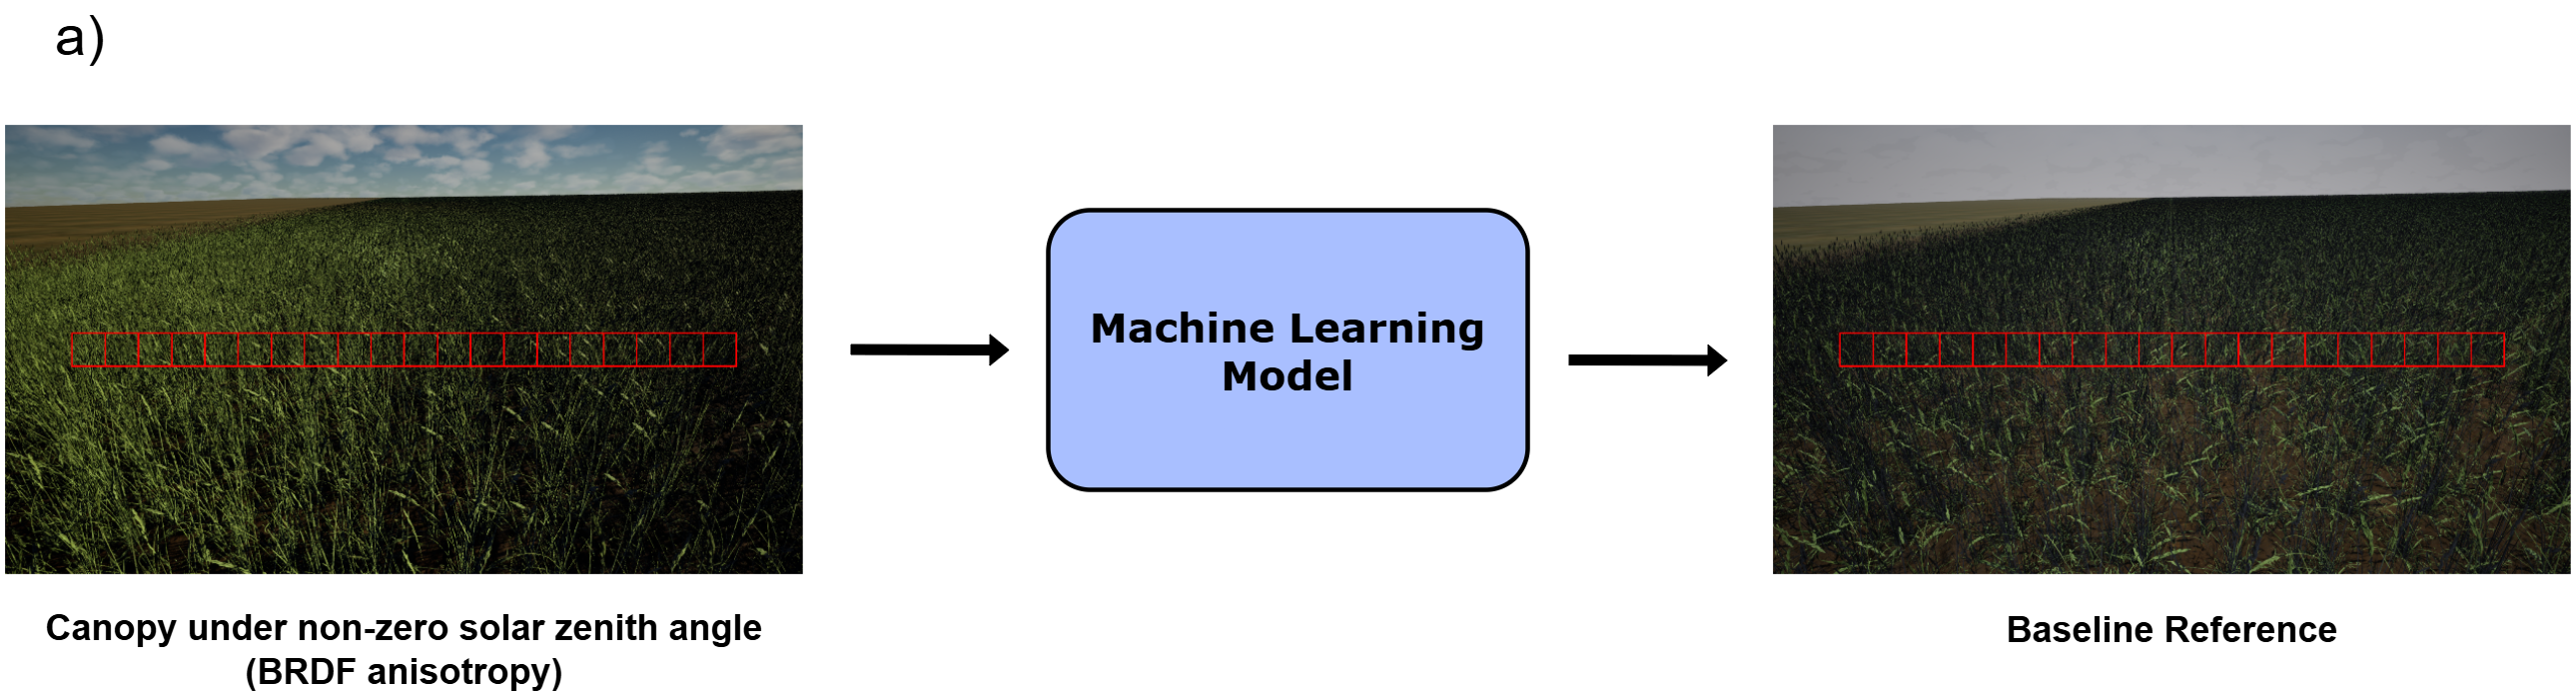
\includegraphics[width=\textwidth]{images/brdf-to-gt.png}
        \caption{First image caption}
        \label{fig1}
    \end{subfigure}

    \vspace{0.5cm}

    \begin{subfigure}{1\textwidth}
        \centering
        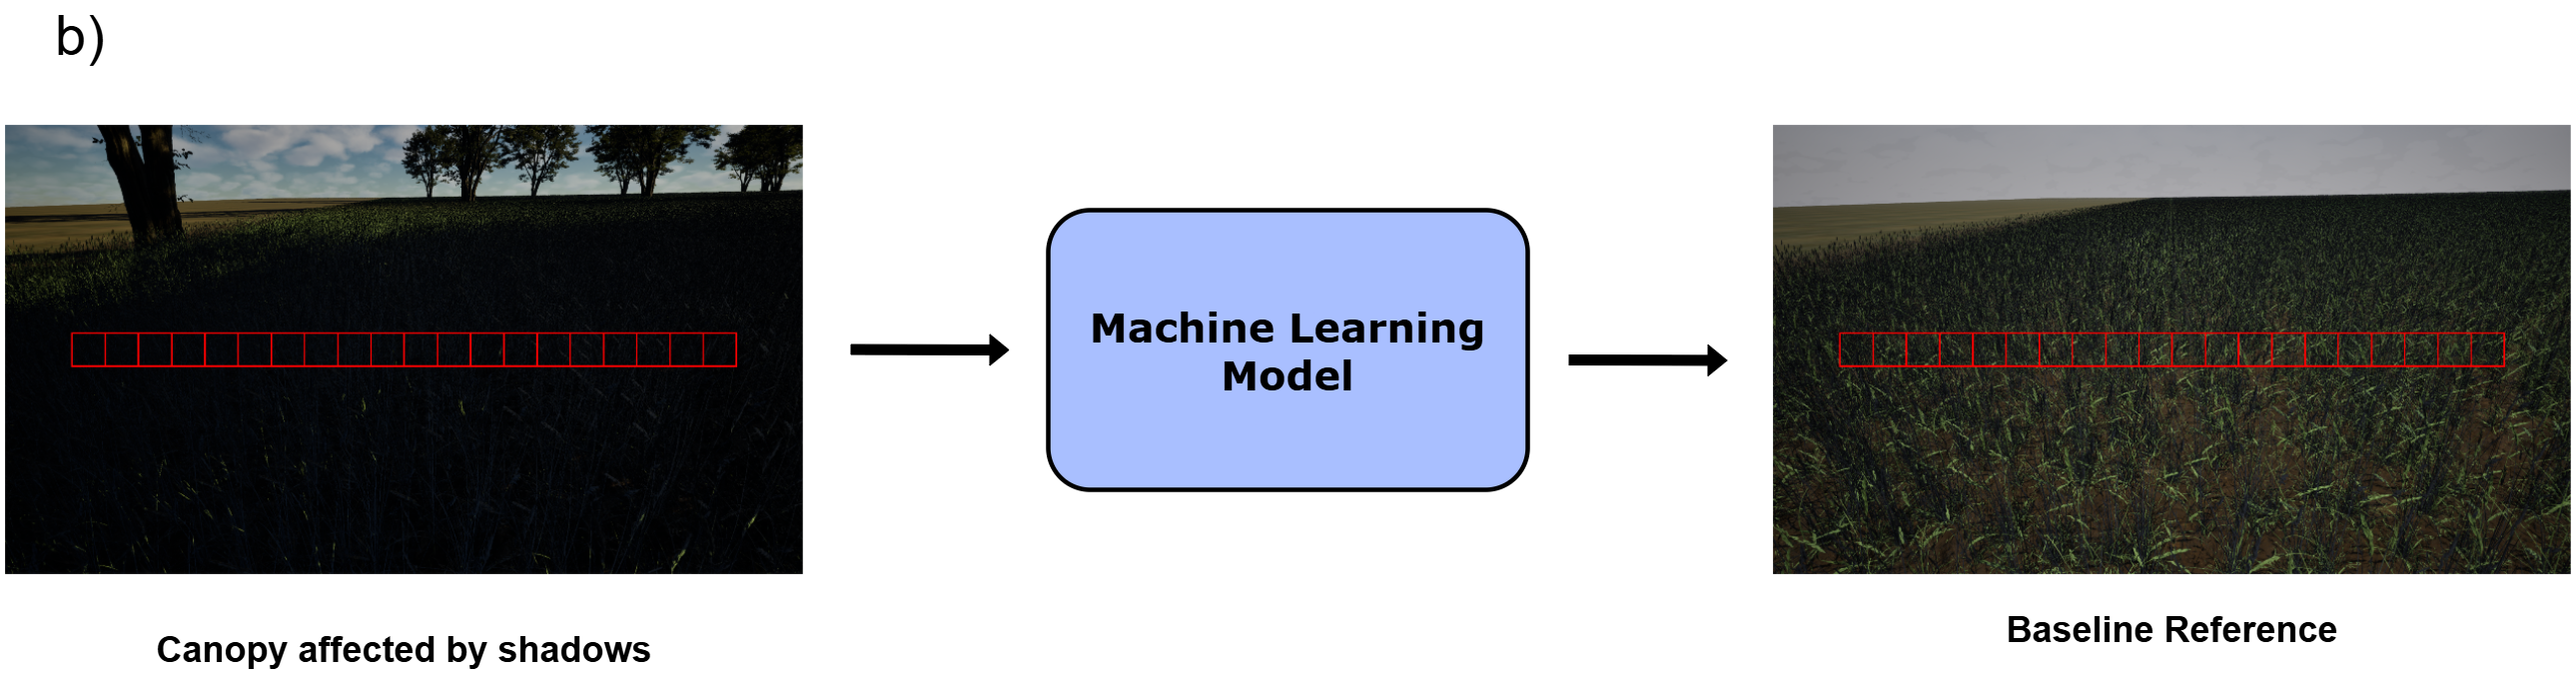
\includegraphics[width=\textwidth]{images/trees-to-gt.png}
        \caption{Second image caption}
        \label{fig2}
    \end{subfigure}

    \caption{The two primary sources of error in this study, excluding errors originating from the sensors used: a) Wheat canopy's anisotropic BRDF, making the sun-sensor-field geometry relevant to the calculated GRVI value and b) The effect of shadows. These factors introduce noise to the perceived material reflectances, and therefore GRVI. Machine learning will be used for approximating the GRVI value under ideal illumination conditions, given the values measured under non-ideal conditions.}
    \label{ml-pipeline-1}
\end{figure} 

The inclusion of machine learning and need for training data introduce an additional challenge to the implementation of the proposed system. Constructing a training dataset would require images captured under ideal weather conditions at different stages of the crops’ growth, serving as the ground truth data which the model will attempt to approach as an output, along with images of the same scenes under non-ideal weather conditions. Collecting such data could be both time- and cost-inefficient, considering the stochastic nature of the weather phenomena.

To overcome this data acquisition barrier, a digital twin of a crop field was developed, becoming the primary data source. By offering control over lighting and atmospheric conditions, material properties and crops growth, digital twins provide a highly robust alternative to physical data collection. Furthermore, advancements in modern graphics, specifically regarding the capacity to render photorealistic digital environments, ensure the viability of synthetic scenes as accurate replications of their real-world counterparts. 


By modeling the studied sources of error influencing GRVI measurements within the digital twin, their individual and combined effects can be characterized and learned by ML models, enabling substantial reduction in measurement variability caused by external conditions. While regressing to values captured under ideal weather conditions removes noise attributed to factors originating from the weather, several other environmental and technological factors persist, including improperly calibrated sensors, the existence of soil in the background and outliers captured during the data collection of the reference baseline. To address these remaining challenges, a second training pipeline is proposed, aiming to approximate directly the GRVI that was assigned to the materials of the virtual meshes before their deployment (Figure ~\ref{ml-pipeline-2}).

\begin{figure} [htb]
    \centering
    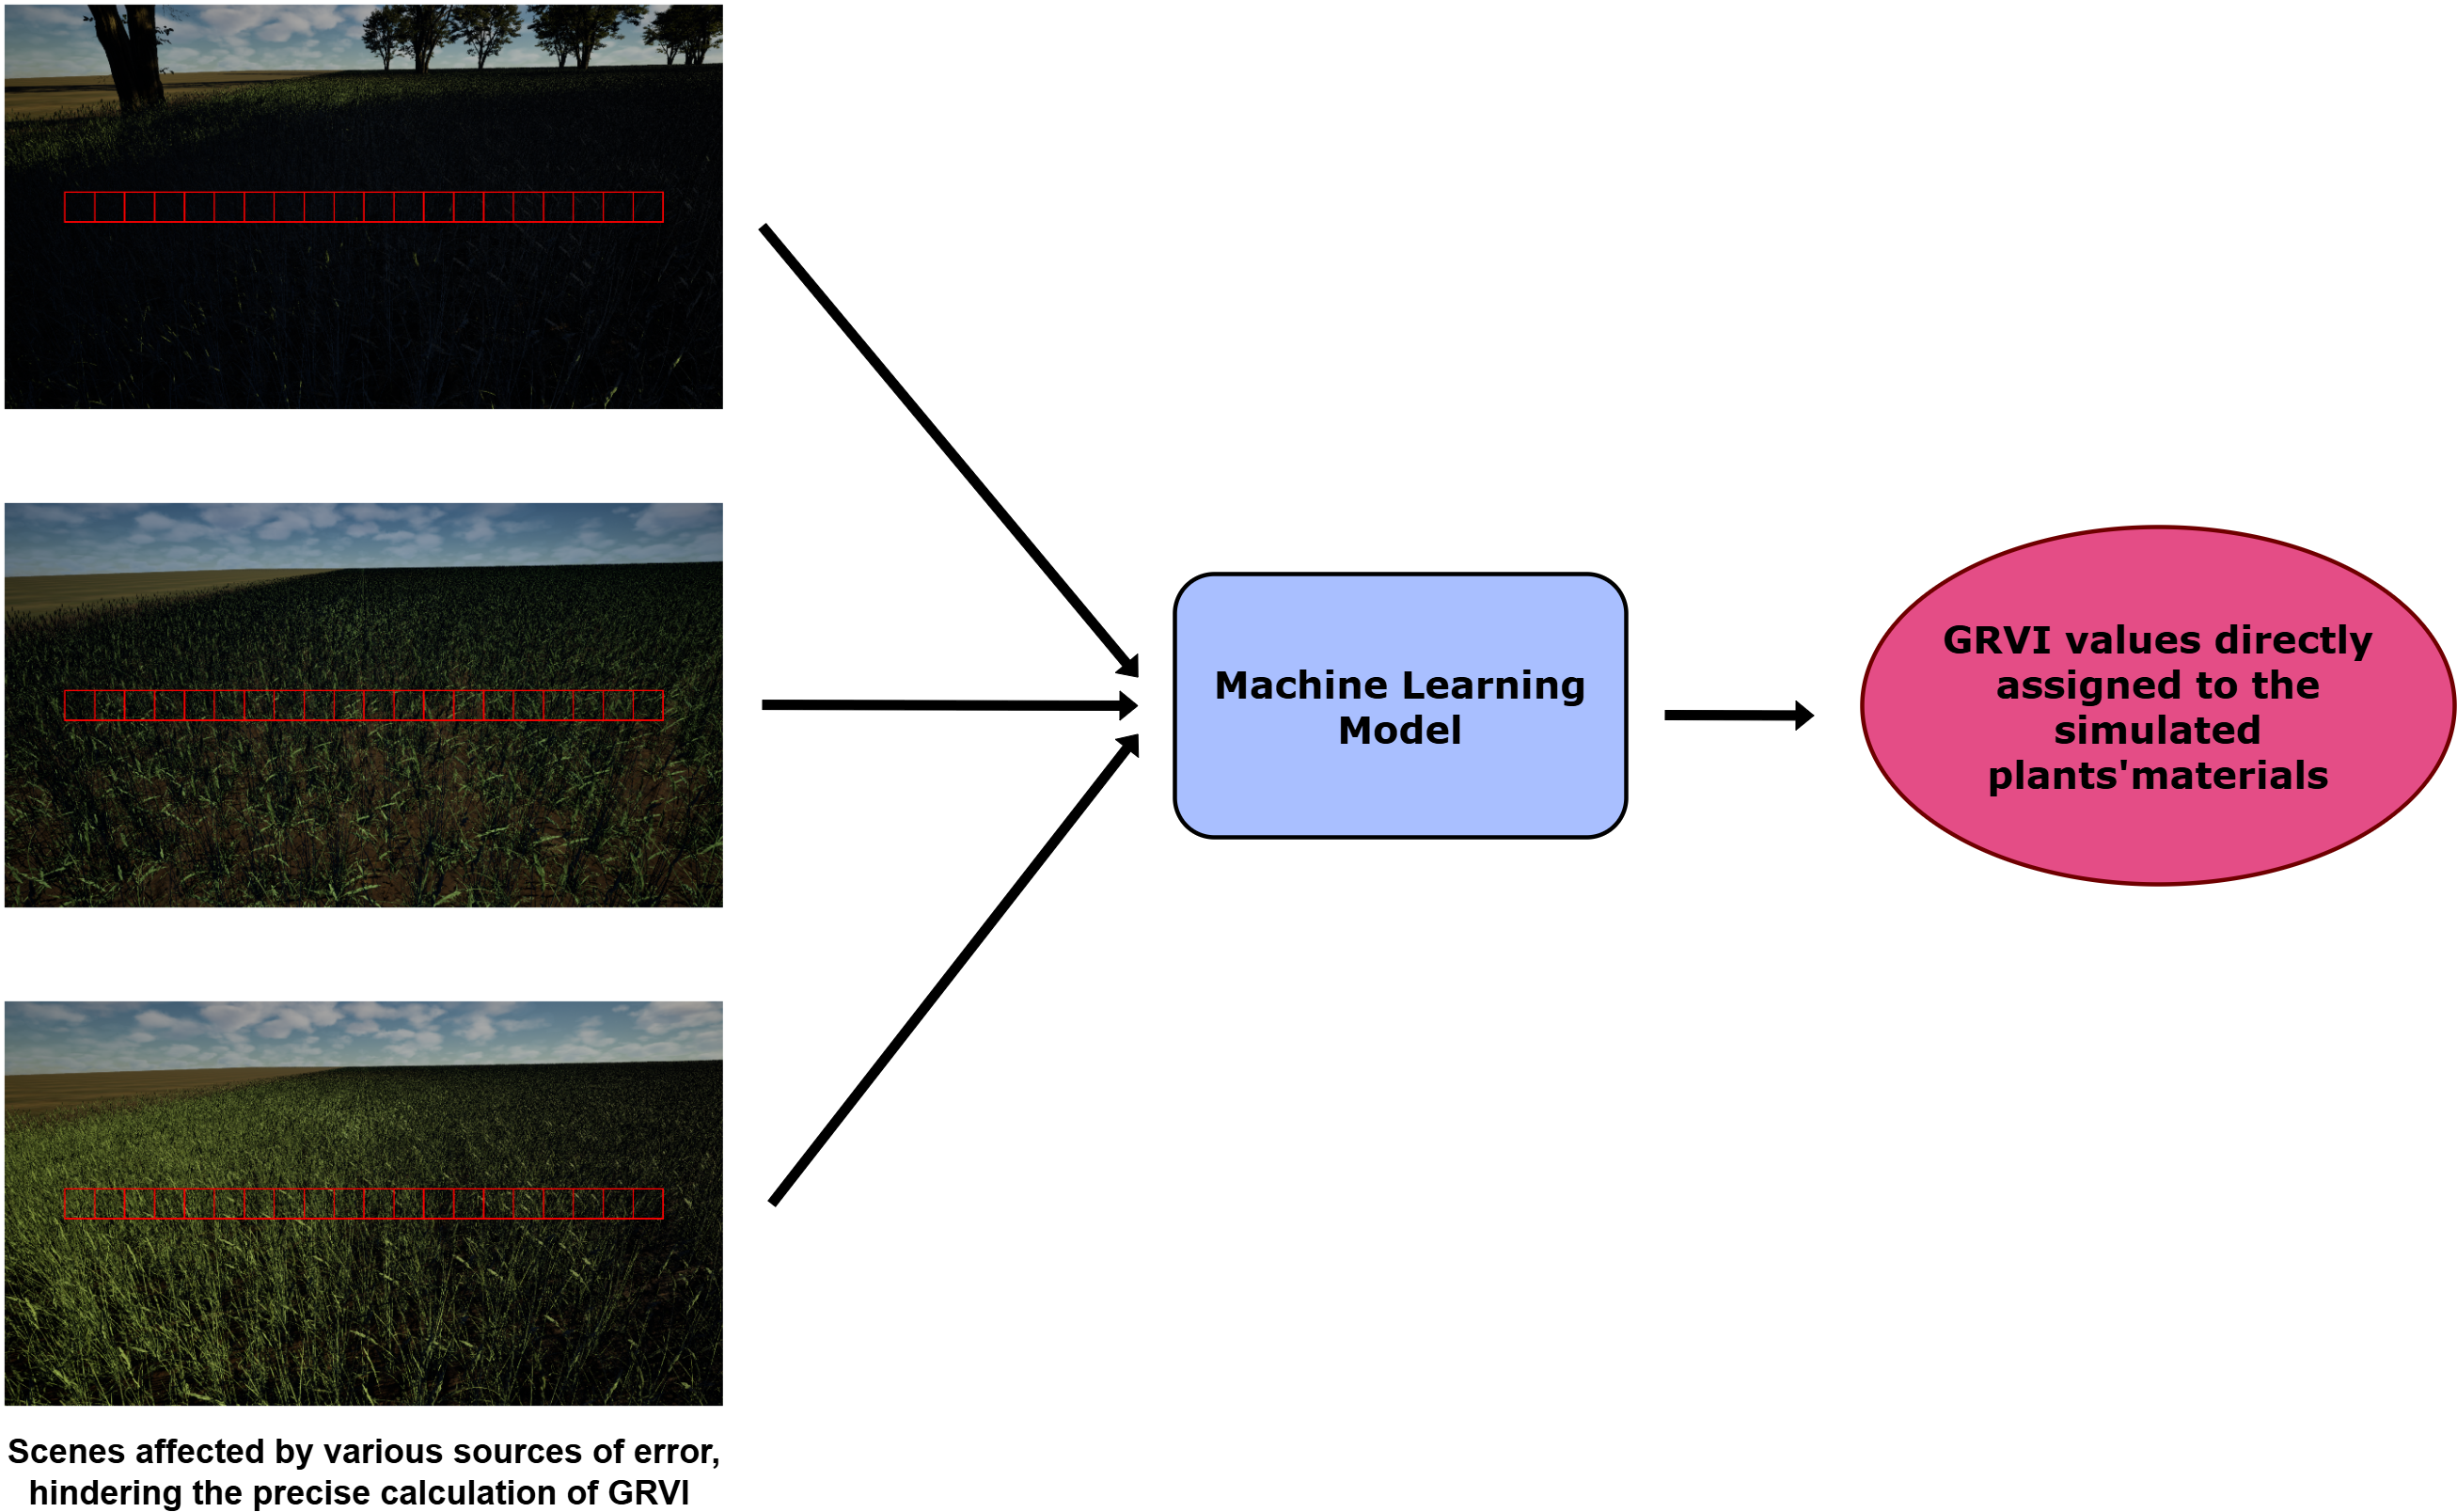
\includegraphics[width=1\linewidth]{images/truegt-pipeline.png}
    \caption{The proposed pipeline for mitigating related to both atmospheric noise and overall environmental and technological factors.}
    \label{ml-pipeline-2}
\end{figure}

\subsection{Contribution}
The main contributions of this work are listed below:

\begin{enumerate}
\item An analytical study identifying the primary factors that cause the perceived reflectance of surfaces to deviate from their actual values.  
\item The development of a photorealistic digital twin of a wheat field in Unreal Engine, specifically engineered to accurately replicate these factors.
\item The creation of tools for automated data collection, ensuring that indexed data (linear images of the scene, the associated illuminance meter readings and camera information etc.) are all both spatially and numerically  aligned.
\item The preprocessing and structuring of the synthetic data into a comprehensive dataset for machine learning applications. 
\item The training and evaluation of various machine learning models on the dataset, designed to regress to GRVI values not affected by weather phenomena, light directionality and viewing geometry. 
\item The identification of an optimal model that successfully balances high predictive performance with low computational overhead, ensuring its viability for edge device deployment.
\item The implementation of a secondary set of machine learning models, designed to approximate GRVI values completely isolated from any source of noise, again, with hardware efficiency in mind. 
\end{enumerate}


\section{Thesis Structure}

This thesis is organized into eight main chapters. In Chapter~\ref{chap1} I define the core challenges this study addresses, introduce the proposed methodological solutions and outline the primary contributions. In Chapter~\ref{chap2} I establish the theoretical foundation by introducing the reader to several key concepts that recur throughout this work. Such concepts include the definition of the spectrometry mechanisms explored, the introduction to Unreal Engine and its involvement in creating synthetic data, and the fundamental machine learning principles used to train the predictive models. Chapter~\ref{chap3} ...

Chapters 4, 5 and 6 are dedicated to presenting the methodology I followed for addressing the identified challenges. In Chapter~\ref{chap4} I detail the implementation of the digital twin in Unreal Engine and introduce the methods used within the digital environment for acquiring information regarding the calculation of a surface's reflectance. In Chapter~\ref{chap5} I describe the stages of the data collection pipeline and the preprocessing of the accumulated data for machine learning applications.
    \chapter{Background}
\label{chap2}

This chapter provides the general framing of the phenomena I investigated throughout this thesis, alongside the tools utilized to either replicate these phenomena within detailed simulations or compensate for their negative effects on the accuracy of the captured data and subsequent algorithmic decision-making. 

\section{Machine Learning (ML)}

 Machine learning is a class of algorithms designed to construct systems that automatically improve through experience. These systems are capable of autonomously learning the underlying relationships between input data and target output, relieving developers from the need to understand these relationships themselves and, eventually, manually modeling complex rules or hard-coding solutions \cite{ml-trends-persp, useful-things-ml}. 

 Early practical applications of machine learning included probabilistic text classification, unsupervised clustering \cite{MacQueen1967SomeMF},  automated decision making \cite{decision-trees} and text recognition \cite{handwritten, lenet}. Over time, the tasks assigned to ML models grew increasingly complex, becoming the dominant methodology for computer vision applications, speech recognition, natural language processing, and more. 

The primary working principle behind the functionality of most supervised ML models is the approximation of a function that, based on its inputs, calculates an output. In parallel, a loss metric is defined, quantifying the error between the model's approximated function's result and the desired output \cite{ml-trends-persp}. Through iterative training, the model gets exposed to multiple examples of input-output pairs, making the approximated function more and more complex and robust to new inputs.

The ability of ML models to autonomously uncover complex relationships and translate them into complex mathematical expressions, without requiring the developer to explicitly define them, was the primary reason why machine learning was elected as the exclusive tool for mapping the measured GRVI values to their ground truth counterparts. Surely, much like many other physical phenomena, the identified sources of error could be modeled and, eventually, a mathematical function could be constructed, handling the calculation of the true GRVI values. By employing machine learning, though, I drastically accelerated this process and yet achieved impressive results.

\subsection{ML Inference on Accelerators and Edge Devices}

Despite the aforementioned advantages of ML, it has its own caveats. One of its most important downsides is that most of the modern widely used model architectures are associated with a high computational cost. During training, many ML algorithms require repeated optimizations over large datasets and high-dimensional parameter matrices, making the training process increasingly demanding as the size and complexity of the model increases \cite{large-scale-ml}. To compensate for the large volume of matrix operations that naturally exceed the practical capabilities of conventional CPUs, researchers have shifted towards parallel platforms for the training of large models.

Computational constrains, however are not limited to the training stage. Once trained, a model must still execute its primary task, with that being providing predictions based on input data. Large models, such as deep neural networks, may contain millions of parameters, requiring large numbers of floating-point operations and memory accesses, leading to increased inference latency, memory usage, and energy consumption \cite{efficient-DNN}. Similar limitations appear in classical ML algorithms, specifically ensemble methods, where increasing the number and complexity of decision trees increases the amount of model information that must be stored and processed. The overhead of these models becomes particularly important when ML models are transferred from powerful workstations to edge devices, where available memory, computational resources, and energy are severely restricted \cite{splitting-stump}. Consequently, reducing the model's size and computational requirements is necessary to enable efficient inference on resource-constrained devices.

Since the final products of this thesis are machine learning models designed for inference in embedded devices, it was important to consider the limitations of these platforms. Therefore, for the design of the final model architectures, compromises had to be made in terms of their complexity, while still achieving promising predictive performance.

\section{Vegetation Indices}

In the context of remote sensing, it has been discovered that analyzing a field's spectral response generally provides the majority of the information needed regarding its vegetation's vigor. That said, relying solely on the raw spectral bands reflected by the field could be unreliable, since these measurements are also influenced by surrounding factors, such as the soil's color, shadows, moisture levels and more. In order to establish a more robust solution for quantifying the intensity of phenomena observed during the monitoring of plants, researchers have developed several mathematical combinations of the distinct spectral bands, known as vegetation indices (VIs) \cite{review-veg-index}. 

The major advantage of using vegetation indices is the ability to monitor complex phenomena occurring during the life cycle of crops, without the need to investigate every contributing variable, while also being isolated from several instances of lingering environmental noise throughout the process. VIs describe aspects of the observed vegetation’s development, such as its growth stage, health status, physiological and environmental conditions, and, in the case of crops, the amount of attention needed per part of the field and the validation of crop uniformity across it by simply quantifying the presence of factors related to these aspects, without the need for further interpretation \cite{vi-in-precision-agr}.


\subsection{Green-Red Vegetation Index (GRVI)}

Green-Red Vegetation Index (GRVI) in particular is a normalized spectral index defined as:
\[
GRVI = \frac{\rho_g - \rho_r}{\rho_g + \rho_r}
\]
where $\rho_g$ and $\rho_r$ are the reflectances of the visible green and red bands, respectively. The most common applications where GRVI is used include plant phenology monitoring.

Compared to other commonly used vegetation indices, such as NDVI, EVI, and GNDVI, GRVI offers several practical and application-specific advantages. Since it relies solely on visible spectral bands, GRVI can be accurately calculated using low-cost visible-band sensors, including properly calibrated RGB cameras \cite{gpp-grvi-phenology}. Beyond being highly cost-effective compared to methods that require expensive equipment, GRVI's reliance on visible radiation also ties it directly to the studied directional lighting phenomena. Visible shifts in the radiation reflected by the crops' canopy actually cause measurable changes to the metric.

Another significant advantage of GRVI relative to other vegetation indices is its sensitivity to visible changes in the vegetation's color. Because of this attribute, GRVI has proven to be effective for monitoring plant greenness across different stages of their lifespan \cite{gpp-grvi-phenology, rs-grvi-phenology}, despite its reliance on less complex systems for its calculation. Considering that part of the development of the digital twin was assigning plants different versions of the same material, creating unevenness in the inherent red-green ratio of the meshes across the simulated field, a metric that would be able to depict this unevenness was needed.

Lastly, another reason for selecting GRVI as the core metric in this work was its susceptibility to atmospheric noise. Especially in ground-based systems, as the one simulated, GRVI values are inconsistent, depending on sun position, cast shadows, viewing geometry, etc. \cite{impact_of_sunlight_conditions}. As discussed later, these factors affected the examined metric during the simulation too. Manipulating them produced a large volume of synthetic data, used as examples of how non-ideal monitoring conditions can harm the extracted information and how, with the use of ML, they can be corrected to approach their true values.

\section{Bidirectional Reflectance Distribution Function (BRDF)} \label{brdf}

The Bidirectional Reflectance Distribution Function (BRDF) describes how incident light arriving from one direction to a surface is reflected towards different directions above this surface. It can also be described as the ratio of the radiance dL($\theta_r$, $\phi_r$) reflected by the surface in the direction ($\theta_r$, $\phi_r$) to the incident irradiance dE($\theta_i$, $\phi_i$) that arrives at the surface due to the source from the direction ($\theta_i$, $\phi_i$). Mathematically:
\[
BRDF = f_r(\theta_i, \phi_i; \theta_r, \phi_r) = \frac{dL_r(\theta_r, \phi_r)}{ dE_i(\theta_i, \phi_i)},
\]
where $\theta_i$ is the incident zenith angle, $\theta_r$ is the reflected zenith angle, $\phi_i$ is the incident azimuth angle and $\phi_r$ is the reflected azimuth angle.

If the reflected radiation changes when the reflected direction ($\theta_r$, $\phi_r$) changes, then the reflector is characterized as anisotropic. The canopy of a crop field behaves as an anisotropic reflector, thus causing the studied phenomenon where different parts of the field appear more illuminated than others. This dependence on the reflected direction is described by the canopy's BRDF.

\begin{figure} [htb]
    \centering
    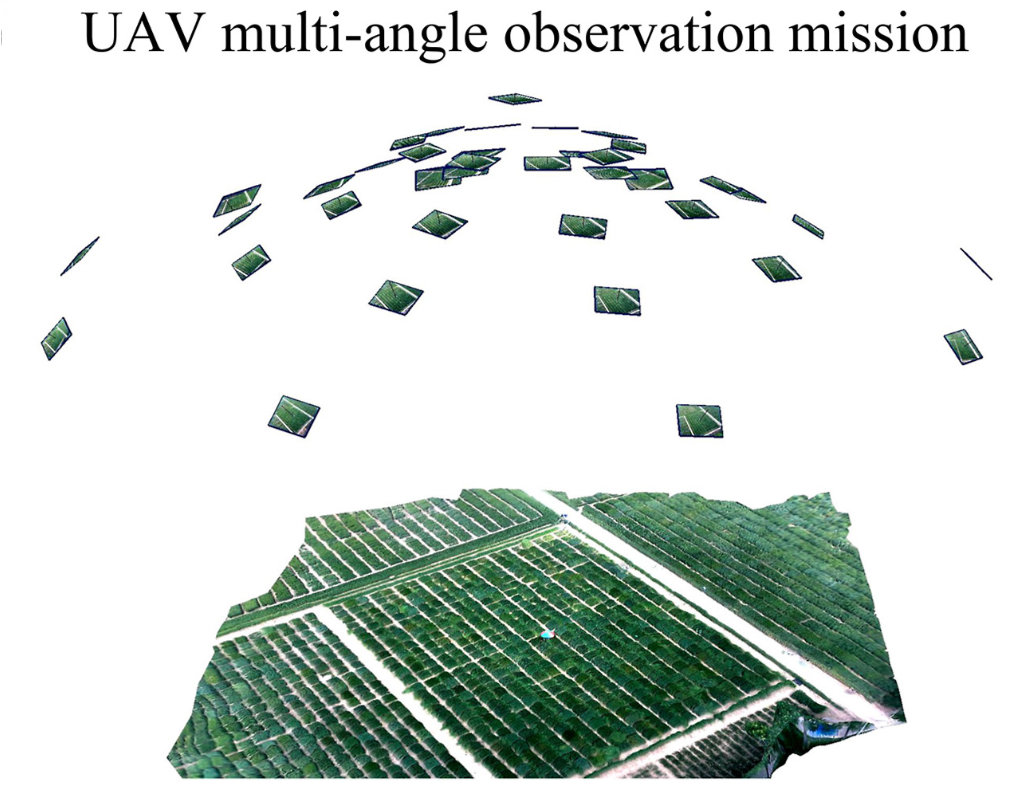
\includegraphics[width=1\linewidth]{images/uav-multiangle.png}
    \caption{BRDF anisotropy examined from various viewing angles with the help of unmanned aerial vehicles (UAV) \cite{uav-bdrf}}
    \label{drones}
\end{figure}

Figure ~\ref{drones} shows a multi-angle UAV observation geometry, proposed by Mi et al. \cite{uav-bdrf} for studying the BRDF anisotropy phenomenon, as it appears on a wheat field's canopy. It can be seen that, depending on the sun-canopy-sensor geometry, several parts of the canopy appear more occluded than others, despite the lack of interference between the light source and the field's canopy.

Multiple instances of this dependence on the illumination source's direction appear in the synthetic dataset, both visually and, most importantly, radiometrically. Depending on the solar zenith angle, a difference as high as 384.79\% could be observed on the average perceived green- and red- band reflectance of the textures appearing in the area of interest, including the errors introduced by the calculation method.

\begin{figure}[htb]
    \centering
    
    \begin{subfigure}{0.48\linewidth}
        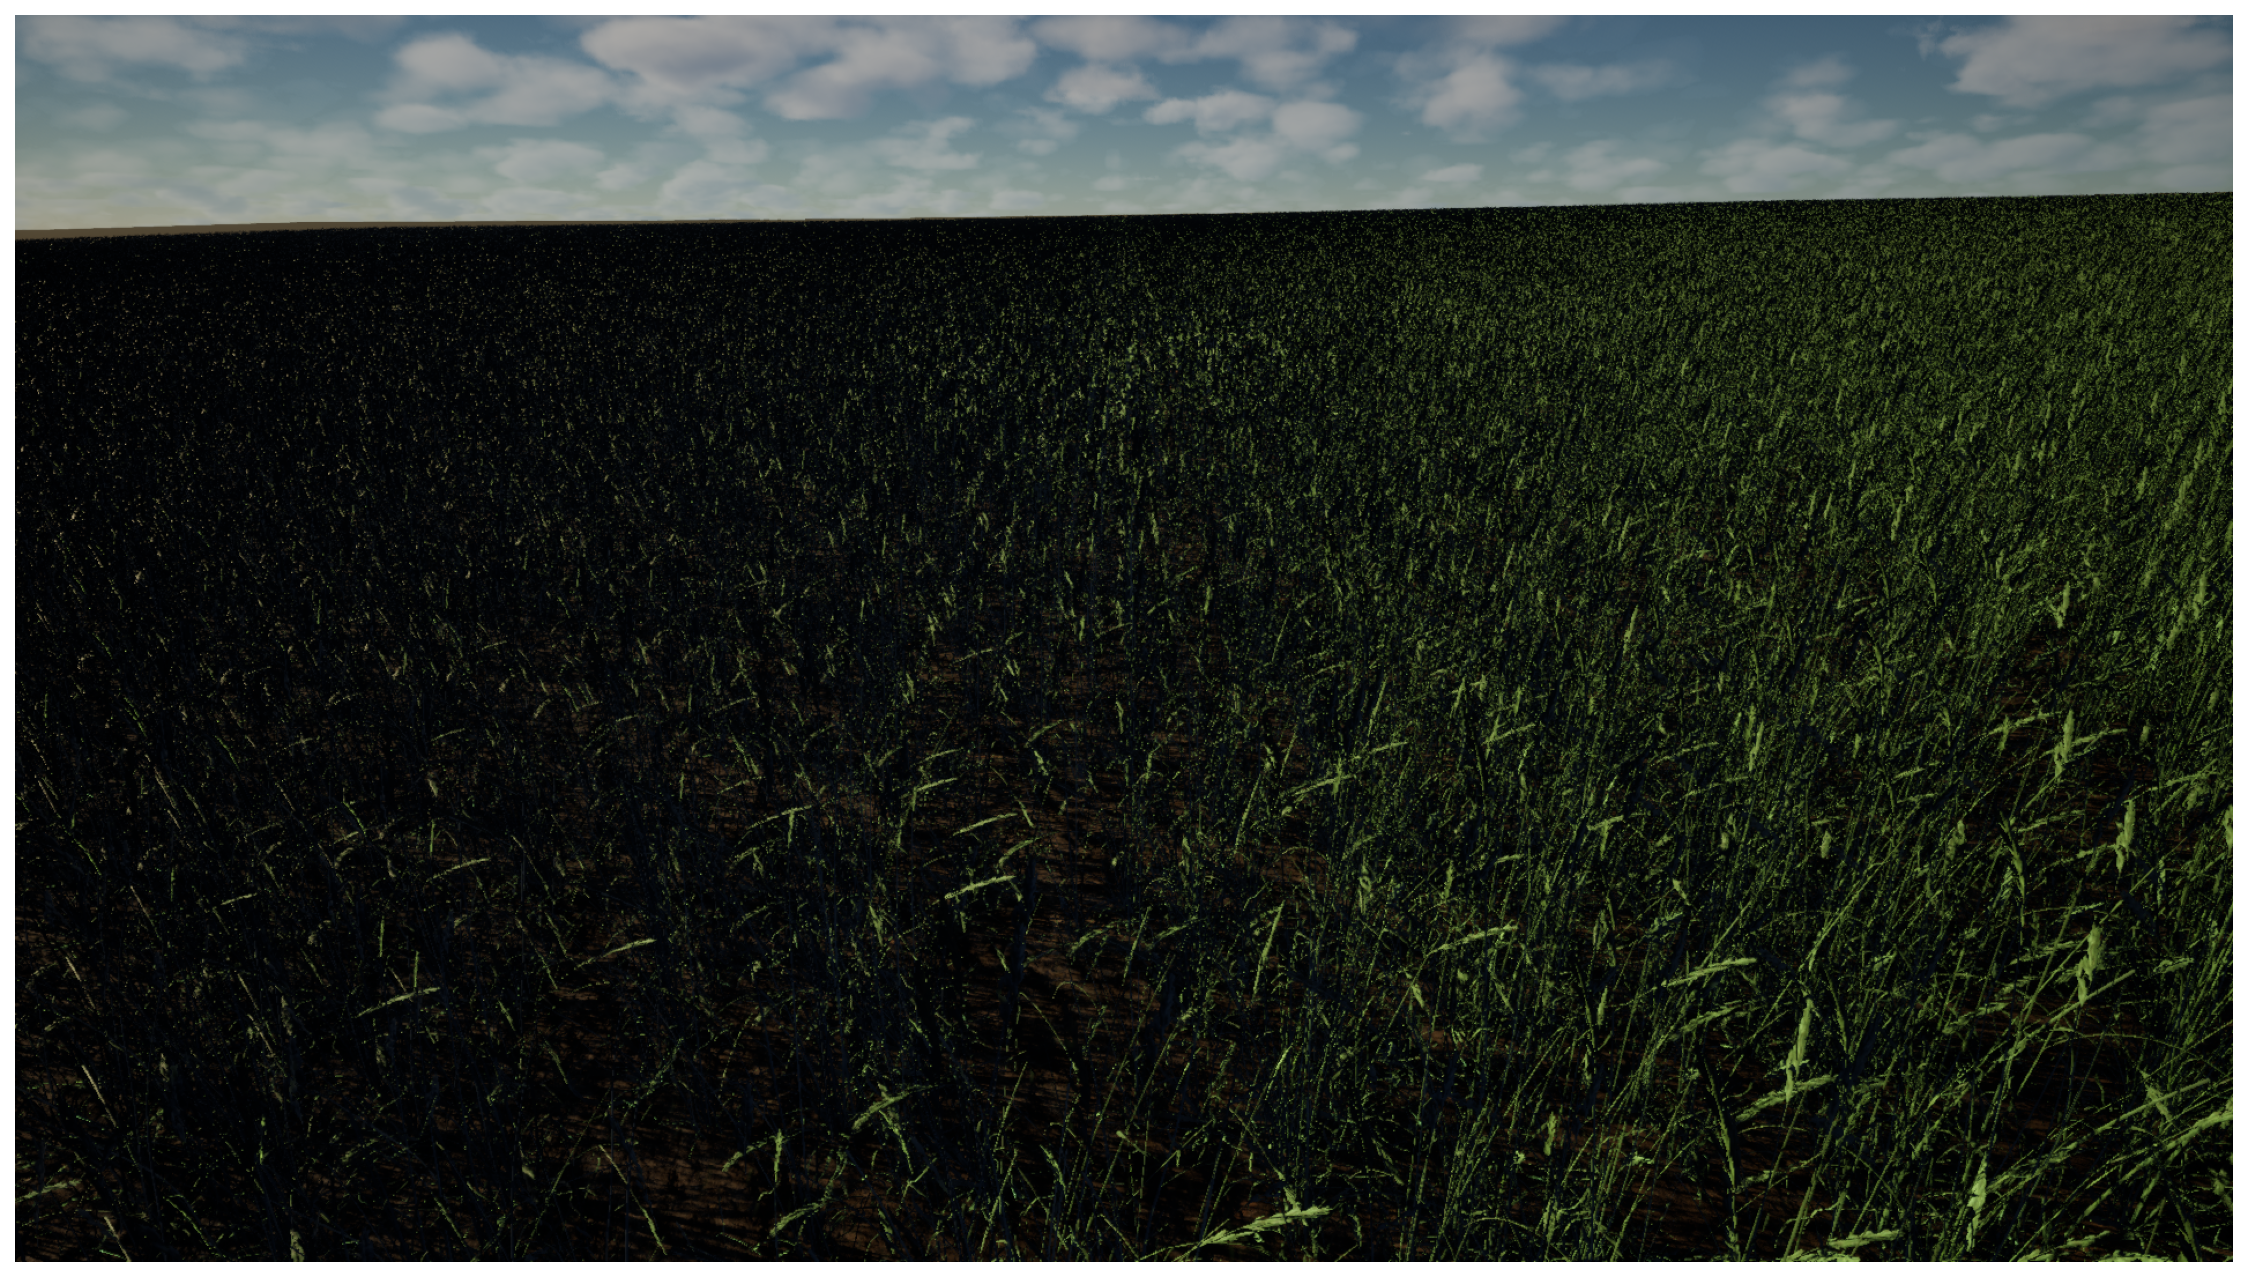
\includegraphics[width=\linewidth]{images/left.png}
        \caption{Image captured with SZA set to $104^o$}
        \label{leftgreen}
    \end{subfigure}\hfill
    \begin{subfigure}{0.48\linewidth}
        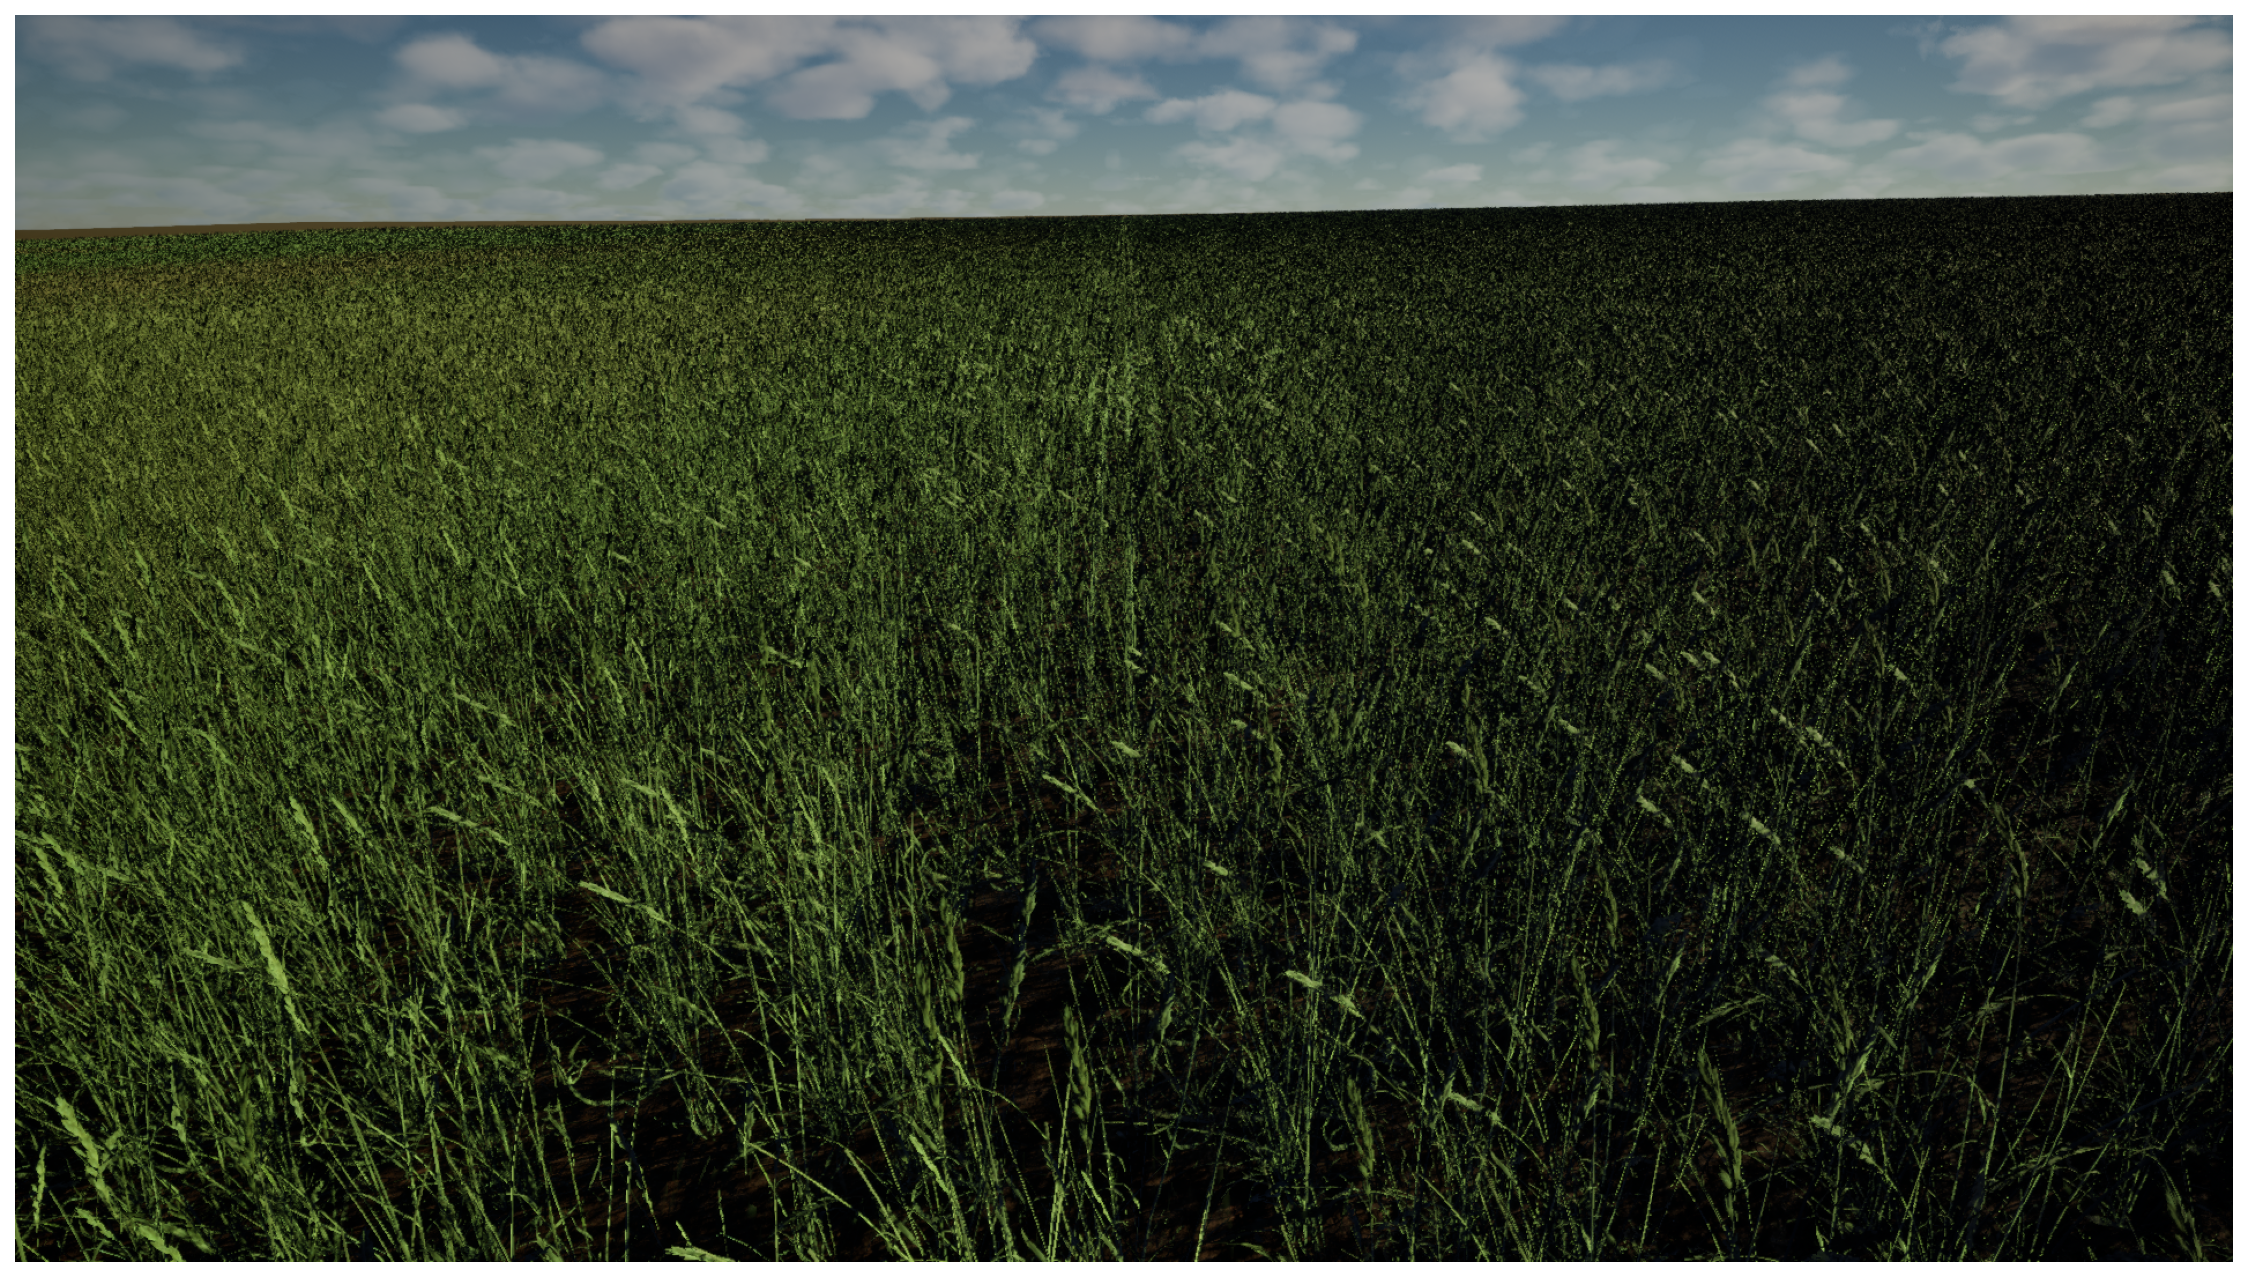
\includegraphics[width=\linewidth]{images/right.png}
        \caption{Image captured with SZA set to $-104^o$}
        \label{rightgreen}
    \end{subfigure}
    
        \caption{Images captured within the digital twin featuring the same scene under solar zenith angles (SZA) with opposite signs. In the left image (Figure~\ref{leftgreen}), the left part of the field appears more occluded than the right, despite the fact that illuminance is proven to be the same across it. The exact opposite is observed in the right image (Figure~\ref{rightgreen}).}
    \label{leftright}
\end{figure}




\section{Tools}
\subsection{Unreal Engine}

Unreal Engine (UE) is a 3D computer graphics game engine developed by Epic Games, capable of generating real-time 3D environments and interactive simulations \cite{wiki:unreal_engine}. In the past few years it has been explored as a digital twin design tool, as it offers a robust set of features, provided either natively or by external plugins, allowing the generation of ground truth data for model training and CV tasks. Apart from its capabilities, UE hosts a large community of developers who use it for digital twin design. This results in a plethora of third-party documentation, plugins, and sensors, all of which sped up the process of environment development and data extraction.

For the purpose of this work, Unreal Engine proved to offer sufficient tools for the implementation of a photorealistic digital environment, the simulation of natural phenomena fairly close to their real-life counterparts and tools capable of both validating these claims and storing the information needed to be gathered for the development of a robust machine learning model. Specifically, UE provides a large library of digital assets, such as foliage meshes and materials, a considerable amount of which are 3D scans of real flora and terrain materials \cite{quixel_megascans}, achieving an impressive level of detail. These assets, accompanied by the engine's built-in tools for procedural, yet not too artificial-looking, mesh placement and terrain manipulation, set an already promising foundation for the development of the environment. In parallel, the engine accurately simulated the various illumination conditions and the resulting light-surface interactions needed for the conducted experiments. Finally, UE supports the automated recording of all of the actors' parameters, especially while a programmed sequence of events occurs, enabling the synthesis of a machine learning dataset. 

\subsection{PyTorch}
PyTorch is an open-source Python library dedicated to the design, training, and inference of machine learning models. It is currently recognized as a standard for deep learning applications, as it combines both an intuitive API and high performance in terms of execution speed, attributed to both its optimized source code and its support for parallel computing platforms like CUDA \cite{torch-intro}. A small extent of PyTorch's capabilities was explored within the bounds of this work for the development of one of the proposed model architectures. 

\subsection{Scikit-learn}
Scikit-learn is an open-source machine learning Python library, widely established as a standard for classical ML, non-neural network algorithms \cite{scikit}. It provides multiple classical ML algorithms, data preprocessing and dimensionality reduction tools, and model evaluation and selection metrics. Scikit-learn was the primary library used for data preprocessing, while several of the algorithm implementations were used in an attempt to identify models that combine computational efficiency and satisfactory results in terms of predictive performance.

\subsection{cuML}
cuML is the scikit-learn counterpart for CUDA-enabled machines. It provides a plethora of classical machine learning algorithms optimized for training and inference on the supported graphical processing units (GPUs) while mimicking scikit-learn's interface \cite{nvidia_cuml_docs}. Apart from the algorithmic implementations of methods that can be found in scikit-learn, such as linear regression, clustering and ensemble algorithms, cuML also provides support for model architectures beyond these bounds. Specifically, the Forest Inference Library (FIL), which is part of cuML, is responsible for optimizing ensemble methods such as XGBoost, LightGBM, and non-inherently supported scikit-learn models for GPU inference \cite{nvidia_fil_2025}. 

cuML was the primary tool used for accelerating non-neural network models, leveraging its GPU-optimized implementations of tree-based ensemble methods. Since the inputs followed the formatting of tabular data, a dataset format where tree-based ensemble methods tend to excel, utilizing this framework ensured high performance both in prediction accuracy and computational speed. 

\subsection{TensorRT}

TensorRT is NVIDIA's SDK for high-performance deep learning inference on CUDA-enabled embedded platforms, such as the NVIDIA Jetson series. By providing a pre-trained neural network in ONNX format to TensorRT, it optimizes the graph by fusing adjacent layers to condense mathematical operations, and applies Post Training Quantization (PTQ), constraining the weights to lower-precision formats (INT8, FLOAT16, etc.) specified by the developer. Finally, it benchmarks multiple kernel implementations per layer and batch size, identifying the best-performing configuration, before compiling the optimized model. The output of this compilation is a file containing the quantized model weights, along with the execution graphs tailored specifically to the platform on which the compilation was performed. The complete compilation pipeline is illustrated in Figure~\ref{trt}, provided by the survey of Jeong et al. \cite{tensor-rt}.

\begin{figure} [htb]
    \centering
    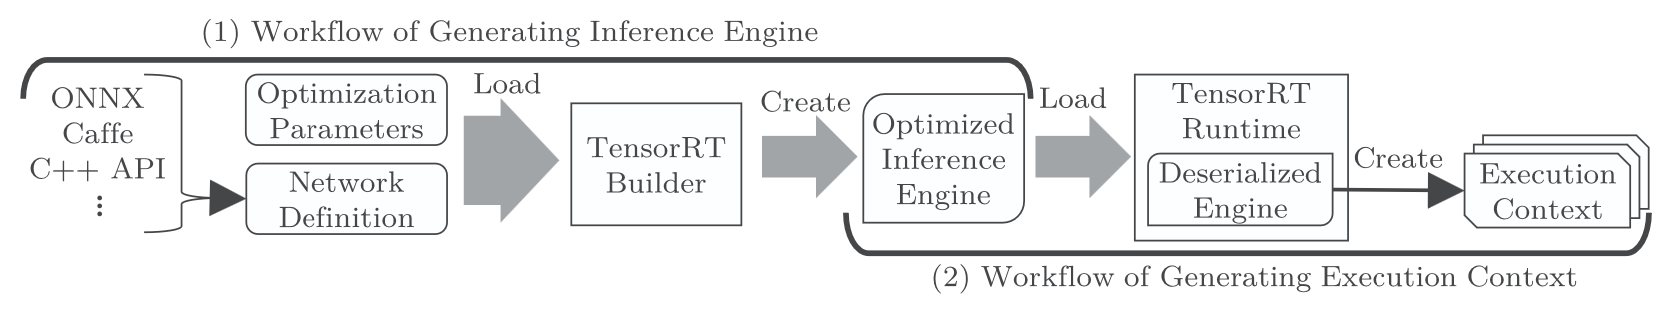
\includegraphics[width=1\linewidth]{images/Screenshot from 2026-09-16 22-44-53.png}
    \caption{Complete optimized model compilation using the TensorRT SDK} \cite{tensor-rt}
    \label{trt}
\end{figure}

Another capability of TensorRT is the profiling of the compiled model, providing performance insights for each individual layer of the compiled neural network.

Although deployment on a Jetson board was not feasible during the course of this research, primarily due to time constraints, experimentation with the TensorRT framework was still conducted. Specifically, the trained neural network models were compiled for execution on an NVIDIA RTX 2060 (6GB VRAM), to evaluate the accuracy loss caused by PTQ.
    \chapter{Related Work}
\label{chap3}



A parallel study was conducted by Qamar et al. \cite{atmospheric-correction-refl}. The objective of this work was to recover true vegetation reflectance, with the primary inputs being the spectral radiance captured by a ground-based remote sensing system and the time and date when the data were collected, without knowing the exact atmospheric conditions present during data collection. Previously implemented algorithmic methods tend to either be highly computationally inefficient, in the case of radiative transfer approaches, or to introduce large uncertainties, depending on the amount of context they are provided with. ML methods, as shown in the work, tend to be relatively computationally efficient while also maintaining a degree of accuracy, even when information such as atmospheric parameters, which in other cases would be necessary, is absent.

To meet the data requirements, the researchers relied heavily on synthetic data. Specifically, they combined simulated vegetation reflectance with simulated atmospheric and solar effects, acquiring the associated at-sensor radiance in the process.  Subsequently, they introduced artificial noise to represent sensor artifacts.

The produced data were used for training a series of Convolutional Neural Networks. The models, given the distorted radiance, output $\Delta reflectance$, the ratio of vegetation reflectance to the median simulated spectrum, which is then used to reconstruct the final reflectance curve. The overall process of data synthesis, model training, and reflectance reconstruction is illustrated in Figure~\ref{rwRef}.

Eventually, the models achieved an $R^2$ of $0.981 \pm 0.004$ when predicting simulated reflectance values. For real-world measurements, the researchers compared the relative reflectance changes predicted by ten independently trained models, expressing a range of uncertainty, with those obtained using the Compound Ratio method. The results showed similar trends in the relative reflectance changes obtained by the two methods.

\begin{figure} [htb]
    \centering
    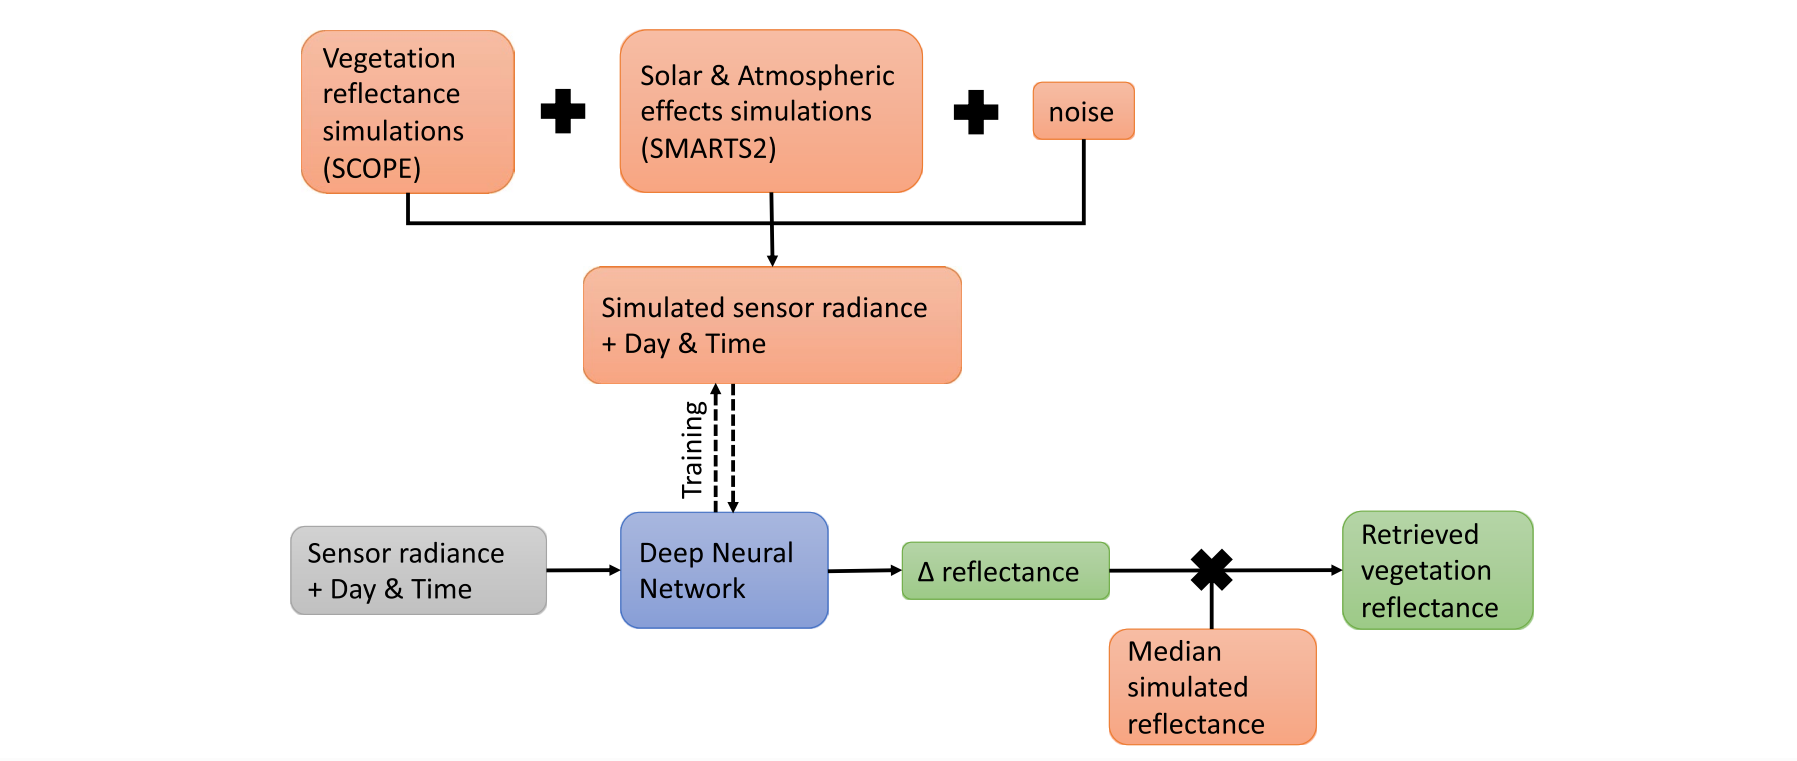
\includegraphics[width=1\linewidth]{images/related-work-1.png}
    \caption{Figure included in \cite{atmospheric-correction-refl}. Depicts an overview of the deep learning framework for retrieving vegetation spectral reflectance from hyperspectral measurements.}
    \label{rwRef}
\end{figure}

Another closely related work was performed by Jasso-Garduño et al. \cite{dl-based-emul}. Within this study, several Deep Neural Network architectures were developed that, given information about the sun-sensor geometry, apparent radiance and Aerosol Optical Depth, were trained to approximate the Earth's surface reflectance. The main motive is to provide an alternative to the computationally expensive radiative transfer methods. The data used for the training of the models were generated using 6S, a radiative transfer model designed to simulate how sunlight interacts with the atmosphere. The best performing model achieved an $R^2$ of $0.995$ when approximating the simulated values. It is important to mention that this this performance was achieved within a specific range of input values, and might need retraining to retain this performance across other scenarios. 


Other related works include those of Siddiqua et al. \cite{macgan} and Joiner et al. \cite{noise-reduct-solar-ind}. In the first one, a Generative Adversarial Network was trained using synthetic data to remove distortion introduced to images by weather phenomena and underwater conditions. In the latter,  ML is used to reduce noise from satellite measurements of terrestrial chlorophyll solar-induced fluorescence. Both simulated and non-simulated data were used for training.

The common source of error across all the aforementioned studies is the influence of uncontrollable parameters when capturing data in outdoor environments, primarily related to atmospheric phenomena and variations in sun-sensor geometry. As in the present study, the proposed solutions for approximating metrics under the desired conditions involve the use of ML models. Given the large amount of data required to train and evaluate such algorithms, the satisfactory performance of models trained on synthetic data and their transferability to real-world data inspired the use of simulations as a data source in the present study.
    \chapter{Development of a Wheat Field Digital Twin}
\label{chap4}

As discussed earlier, in order to address the main challenge of illumination variability, a consistent source of data should be identified beforehand. For this study, I developed a digital twin of a wheat field designed to provide all the data necessary for the construction of a training dataset. Specifically, considering the need to simulate several illumination scenarios, the objective was to prepare three versions of the digital twin:

\begin{itemize}
    \item one with \textbf{cloudy sky}, simulating diffuse lighting conditions. Within this version, the reference GRVI values were collected
    \item one with \textbf{clear sky} and parametrized sun position, enabling captures of the scene for multiple discreet lighting configurations
    \item one with \textbf{clear sky} and the addition of trees, introducing \textbf{shadows} to the scene, while sun position remains variable 
\end{itemize}

% add  block diagram

\section{Design Implementation}

This section provides a detailed description of each asset or pipeline employed during the wheat field's digital twin development.

\subsection{Ground Setup}
The setup of the ground directly affects the quality of the produced data. Since the area of interest in a captured scene does not solely consist of the field’s canopy but rather includes the surrounding soil as a background, the appropriate selection of materials and their adjustments are crucial. This way, the renders appear more natural and realistic in terms of coloration, roughness, and albedo, making the extracted information meaningful. Ground displacement also plays a role in the perceived reflectance calculation. By simulating subtle height variations of the soil, the canopy illumination is affected by the shadows cast, depending on the position of the sun. Introducing variations of these parameters in the training examples can enhance the robustness of the algorithm by increasing the diversity of the input data. For these reasons, I dedicated a part of the digital twin’s development to designing the soil.

\begin{figure}[htb]
    \centering
    
    \begin{minipage}{1\textwidth}
    
        \begin{subfigure}{0.48\linewidth}
            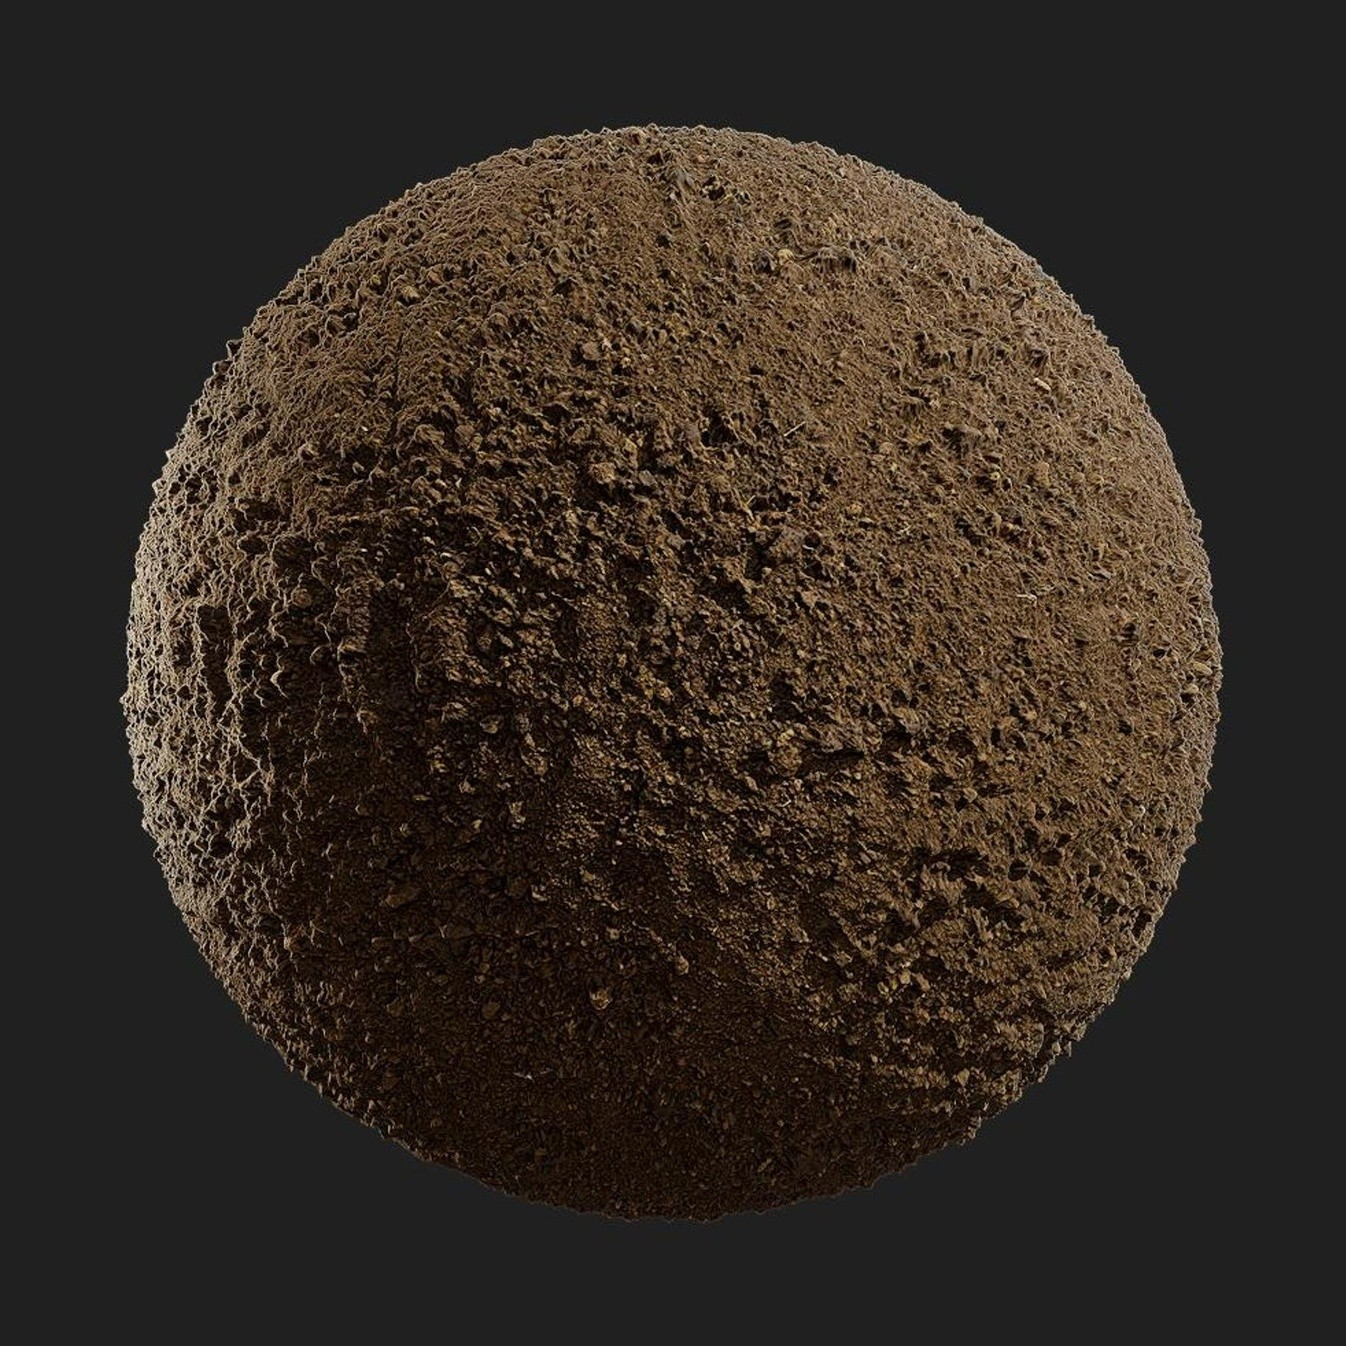
\includegraphics[width=\linewidth]{images/soilmud.jpg}
            \caption{"Soil Mud" material}
        \end{subfigure}
        \hfill 
        \begin{subfigure}{0.48\linewidth}
            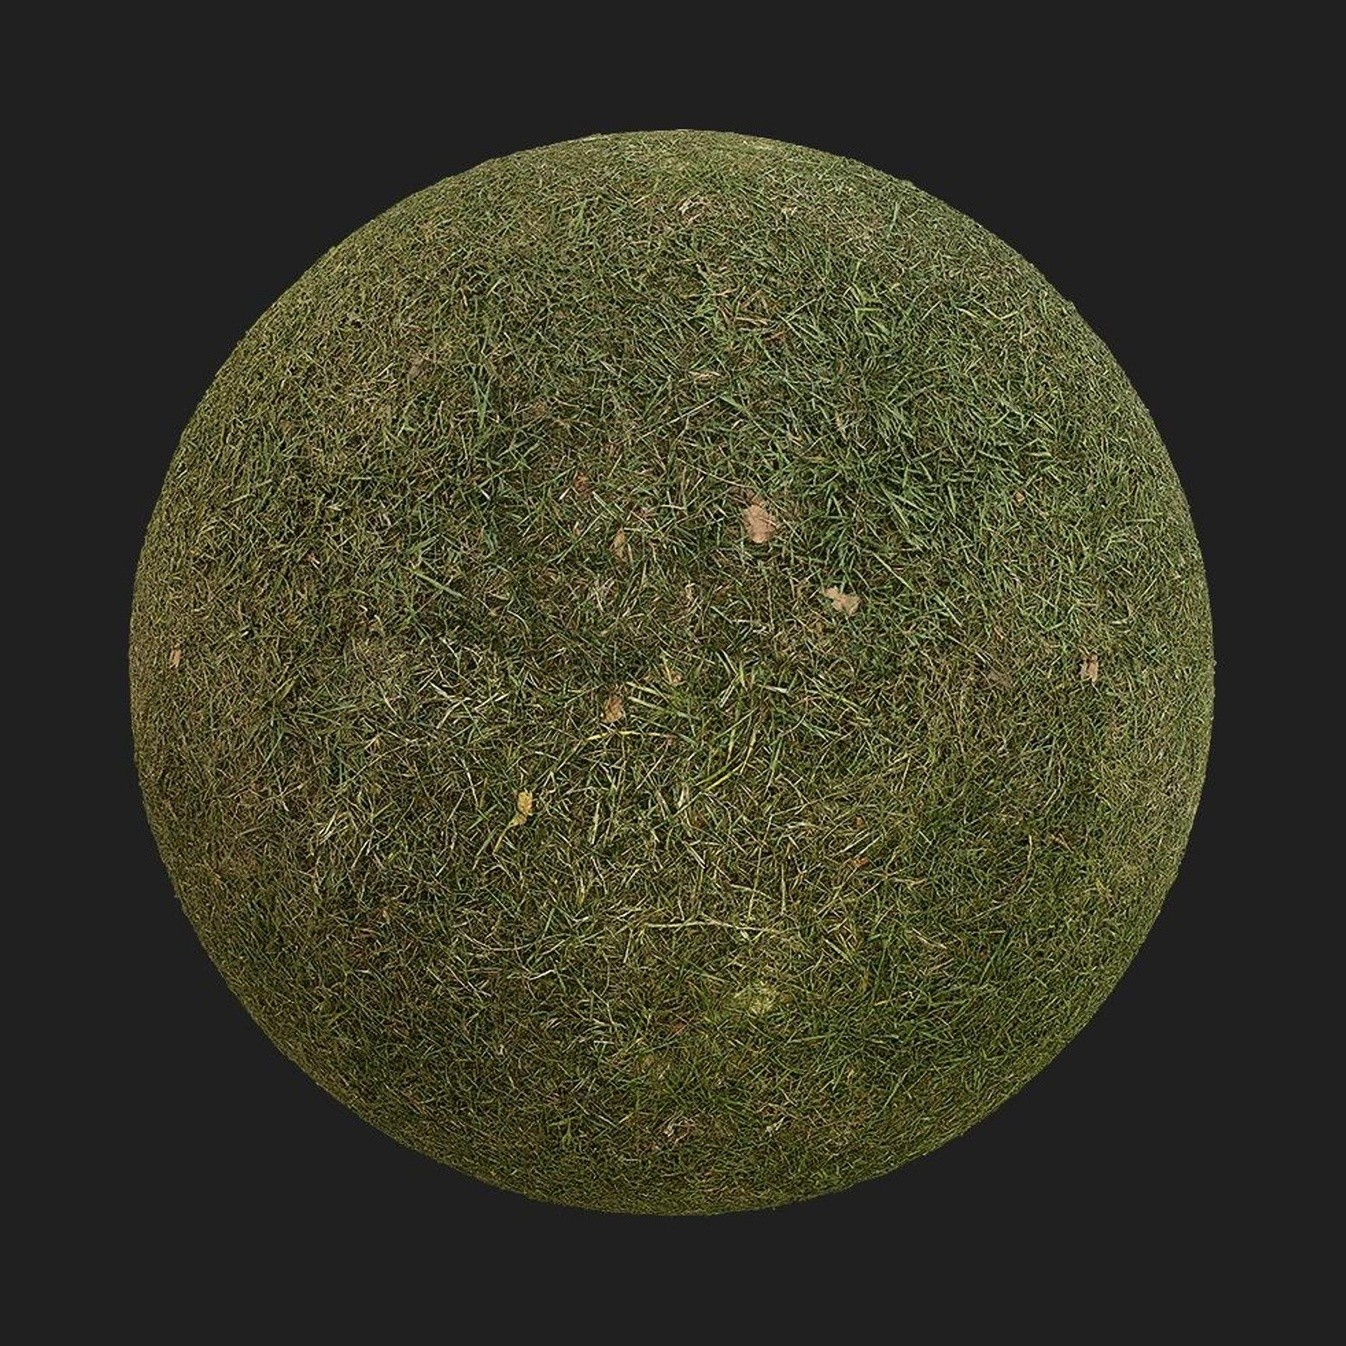
\includegraphics[width=\linewidth]{images/grass.jpg}
            \caption{"Lawn Grass" Material}
        \end{subfigure}
        
        \vspace{1em}
        
        \begin{subfigure}{\linewidth}
            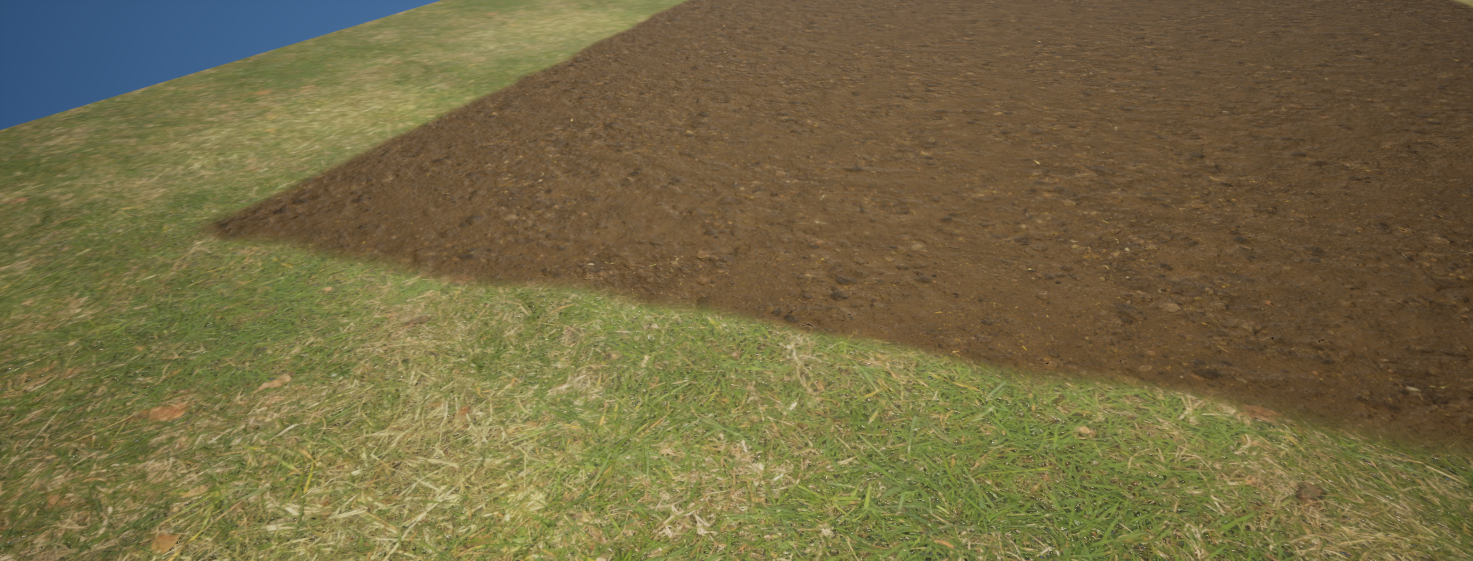
\includegraphics[width=\linewidth]{images/blendedground.png}
            \caption{Landscape actor with blended-ground material applied}
        \end{subfigure}
        
        \caption{The materials used for the digital twin's terrain, both isolated and combined.}
        \label{mat-blend}
        
    \end{minipage}
    
\end{figure}

\subsubsection{Materials}

For the terrain within the crop field, I used ”Soil Mud” \cite{quixel_soil_mud_fab}, signifying the existence of bare soil and crop vegetation, while for the surrounding area I used ”Lawn Grass” \cite{quixel_lawn_grass_fab}, simulating short grass. Unreal Engine allows further processing of the selected materials, enabling the display of several different variations of the same scene. Specifically,  by introducing weights to the texture components that define each material, the ground can be more or less reflective by altering its roughness, implying different levels of moisture present, along with the overall surface brightness, by adjusting the respective RGB intensity values. I exposed the material parameters to UE's interface during the digital twin development for quicker and more intuitive access but did not alter them during the data accumulation.

Assigning different materials on UE’s Landscape actor was achieved by using material blending. In this context, this process includes creating a multilayer material, enabling different textures to be applied by simply drawing one on top of the other. I manually performed the blending, as the manual painting of the landscape appeared to be a more straightforward yet precise workflow. The applied blended material is illustrated in Figure~\ref{mat-blend}.


\subsubsection{Landmass}

The Landmass Plugin is a procedural tool, designed to edit UE’s Landscape actor \cite{epic_landmass_building_worlds}. Its ability to stochastically shape the ground, creating height variations across it, is particularly relevant, since height differences across the terrain can cast shadows, introducing noise to the measurement of a surface's GRVI. Considering that agricultural fields should be relatively flat, the intensity of the displacement that could be applied is limited. Yet, even for the lower levels of displacement, the impact on the shadows was noticeable (Figure~\ref{landmass-int}).

\begin{figure}[htb]
    \centering
    
    \begin{minipage}{1\textwidth}
    
        \begin{subfigure}{0.32\linewidth}
            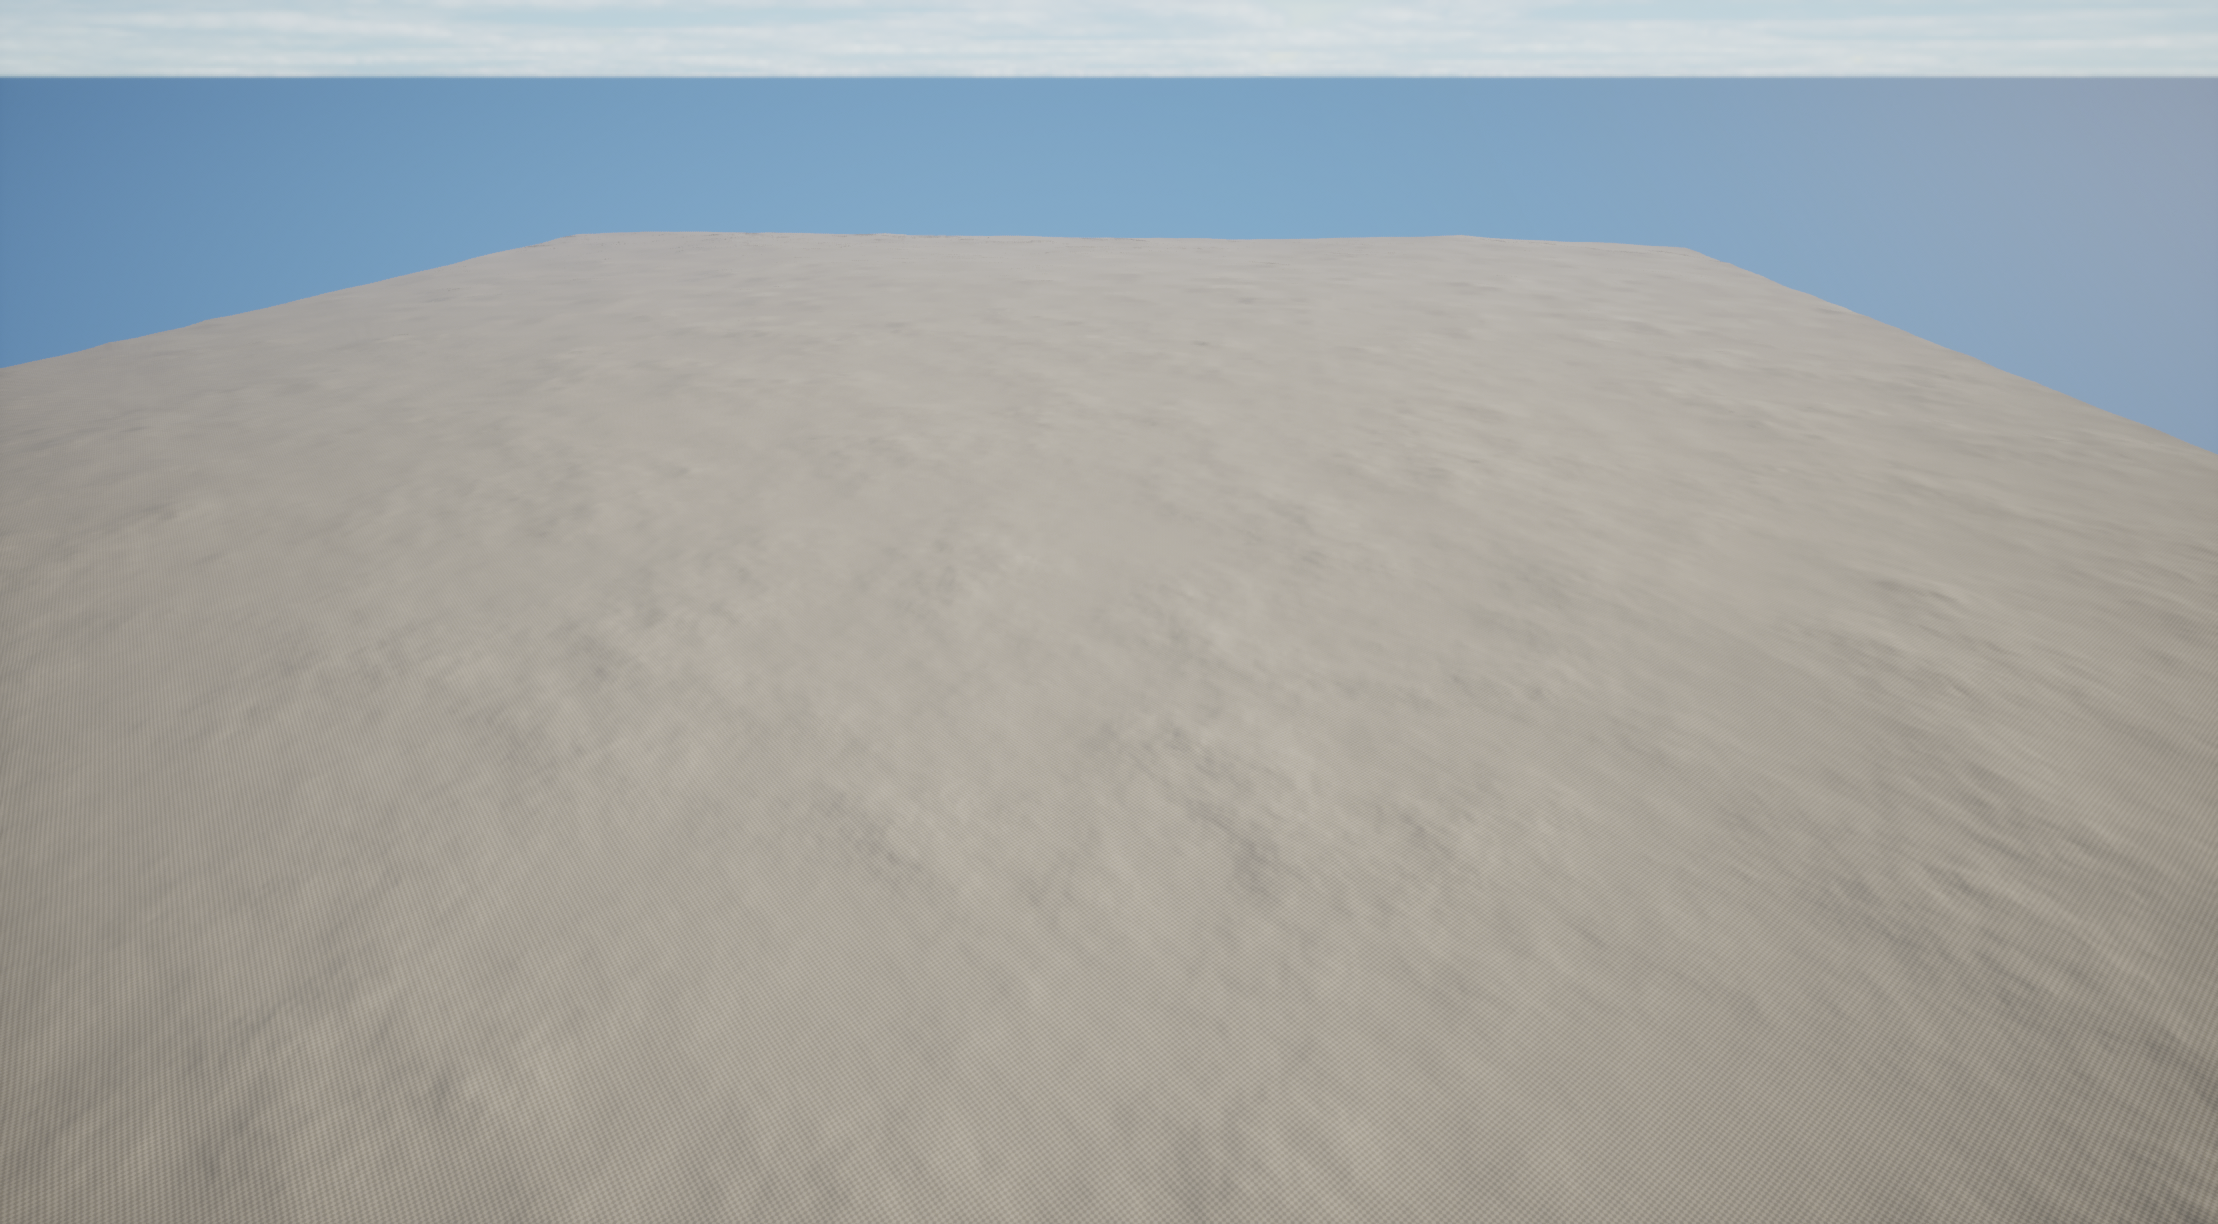
\includegraphics[width=\linewidth]{images/noise600.png}
            \caption{Disp. Height: 600}
        \end{subfigure}\hfill
        \begin{subfigure}{0.32\linewidth}
            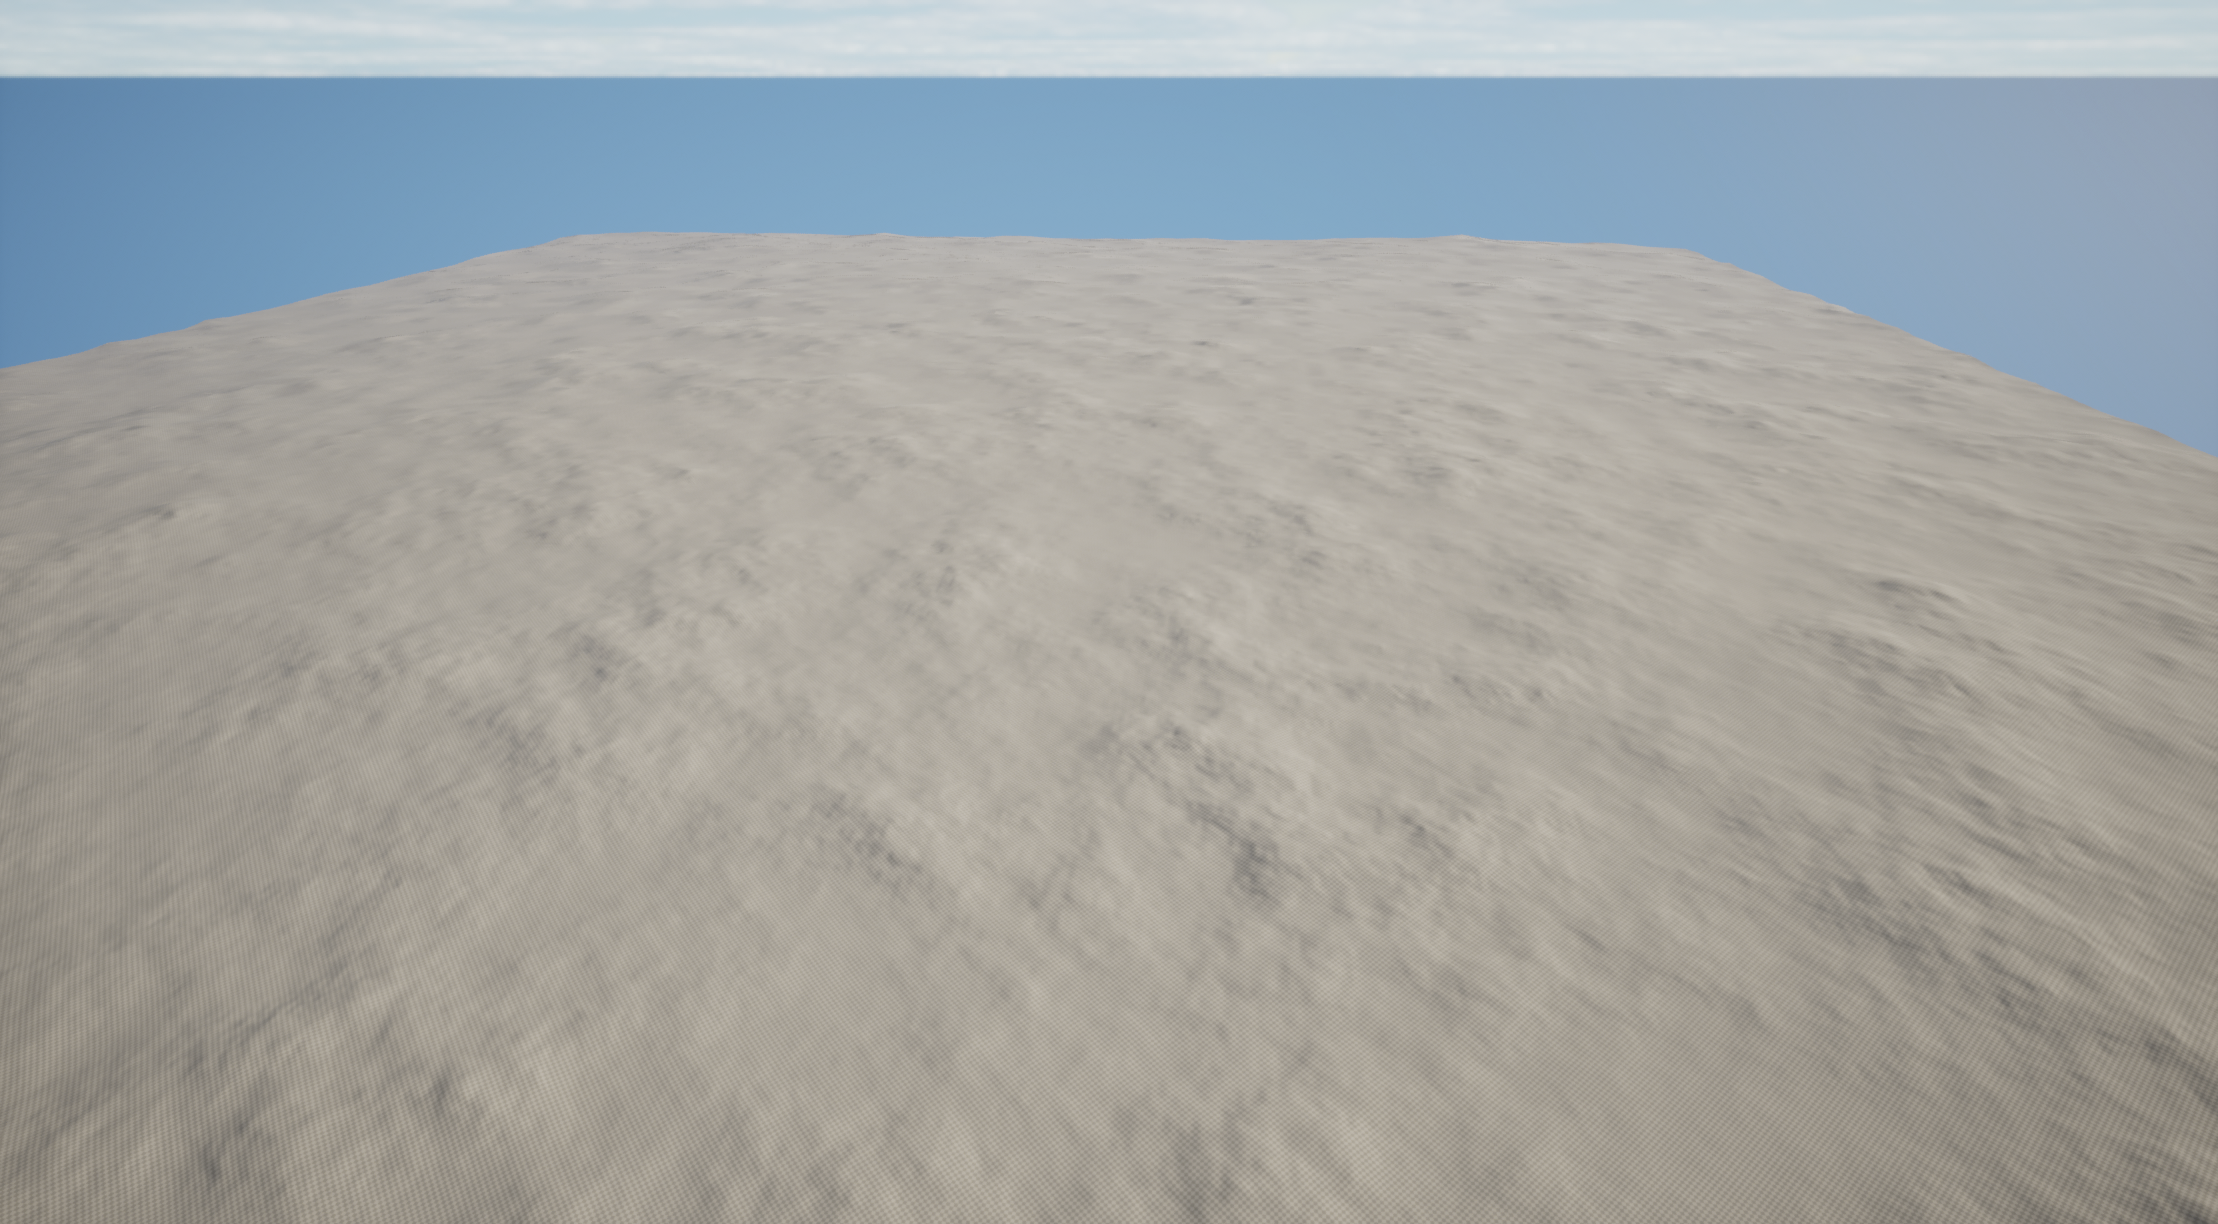
\includegraphics[width=\linewidth]{images/noise1200.png}
            \caption{Disp. Height: 1200}
        \end{subfigure}\hfill
        \begin{subfigure}{0.32\linewidth}
            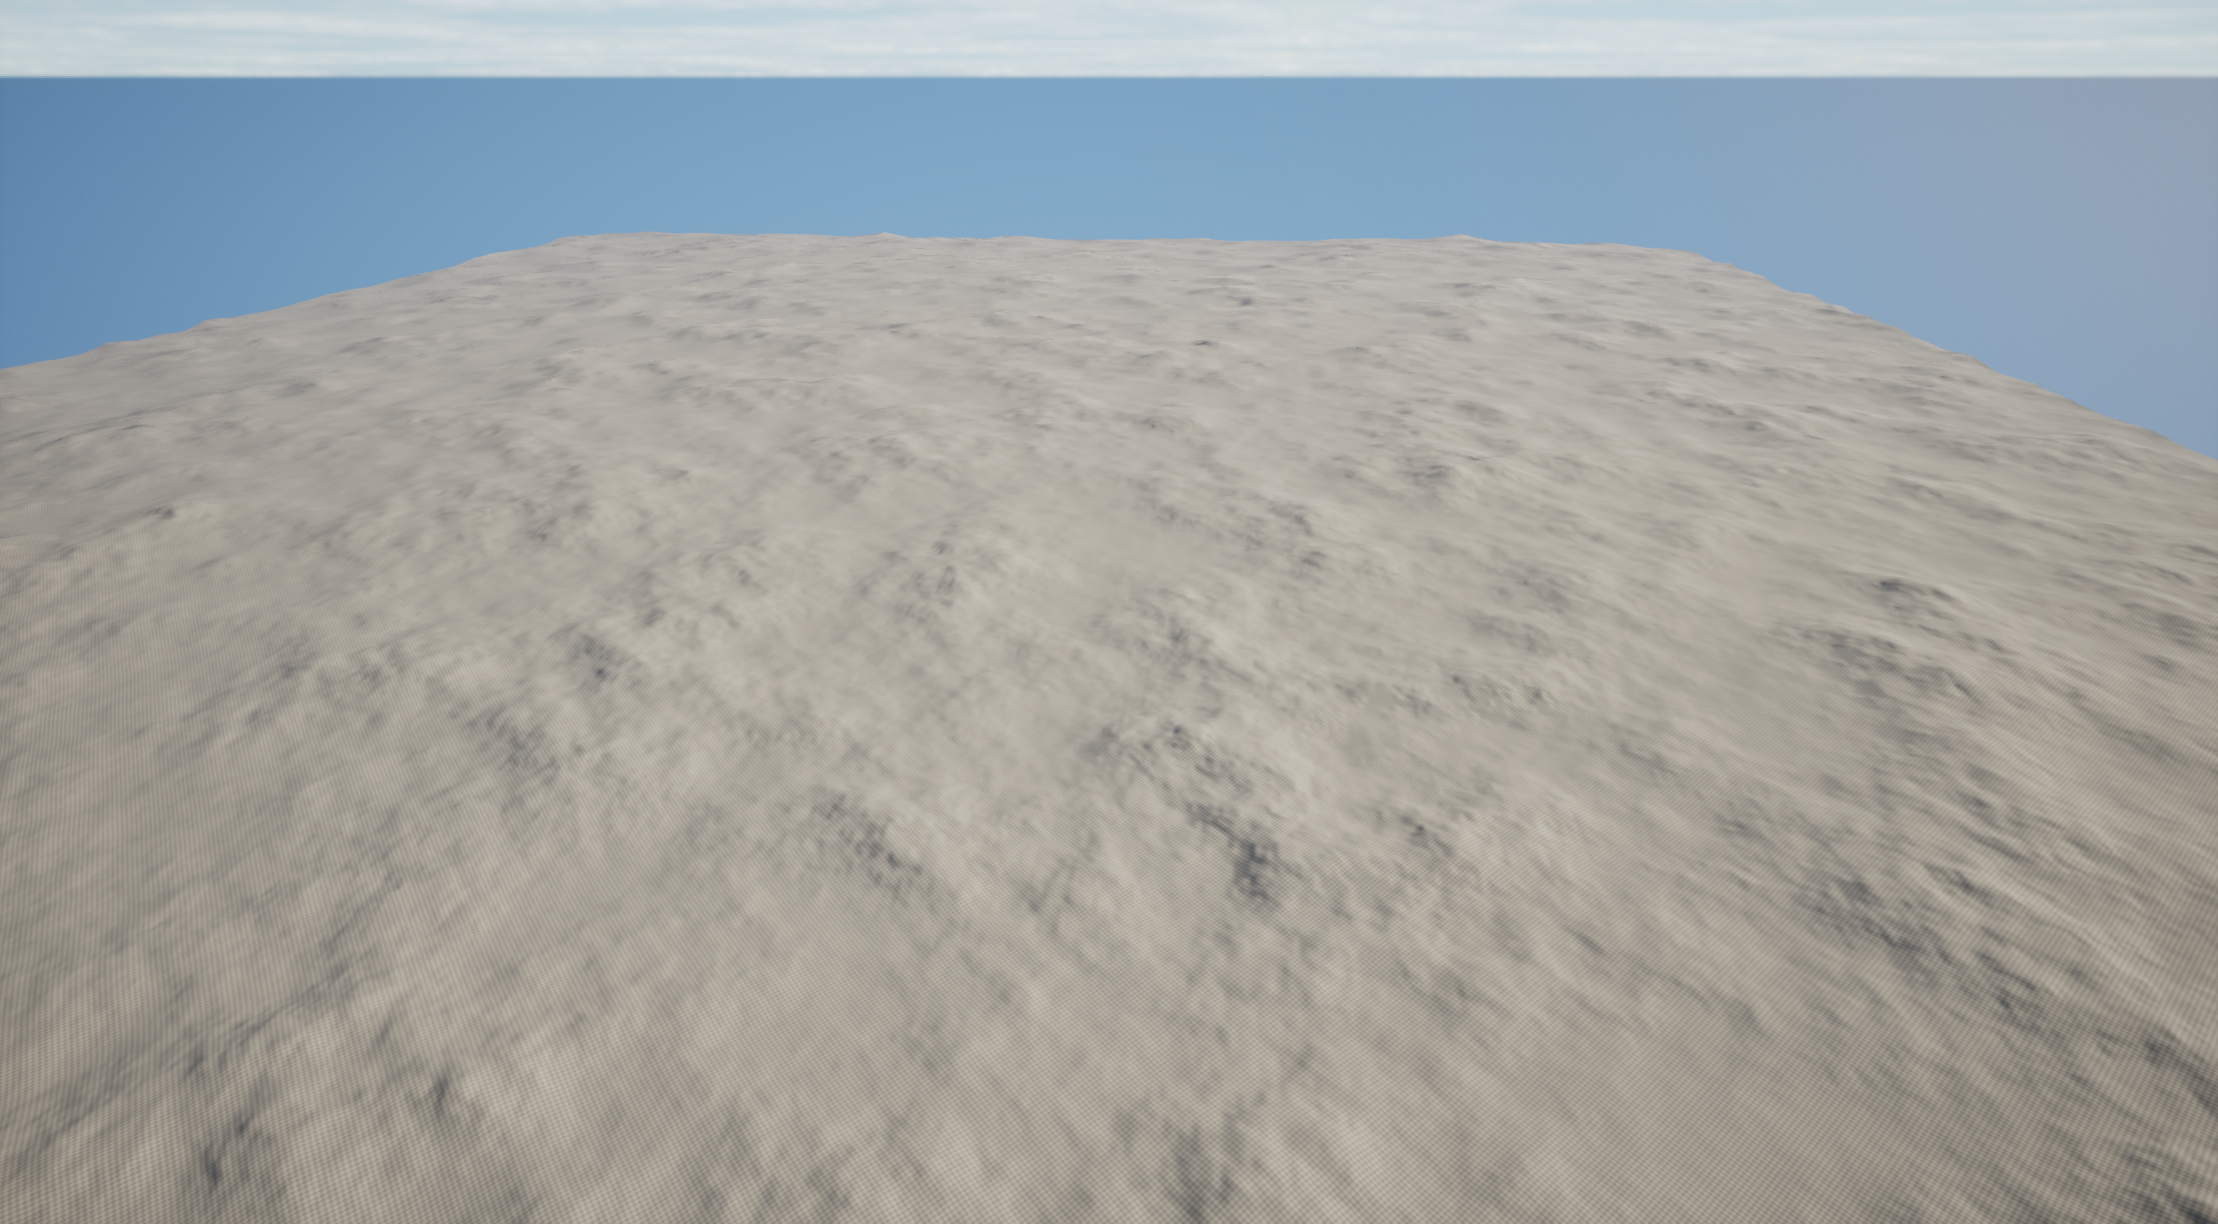
\includegraphics[width=\linewidth]{images/noise1800.png}
            \caption{Disp. Height: 1800}
        \end{subfigure}
        
        \vspace{1em}
        
        \begin{subfigure}{\linewidth}
            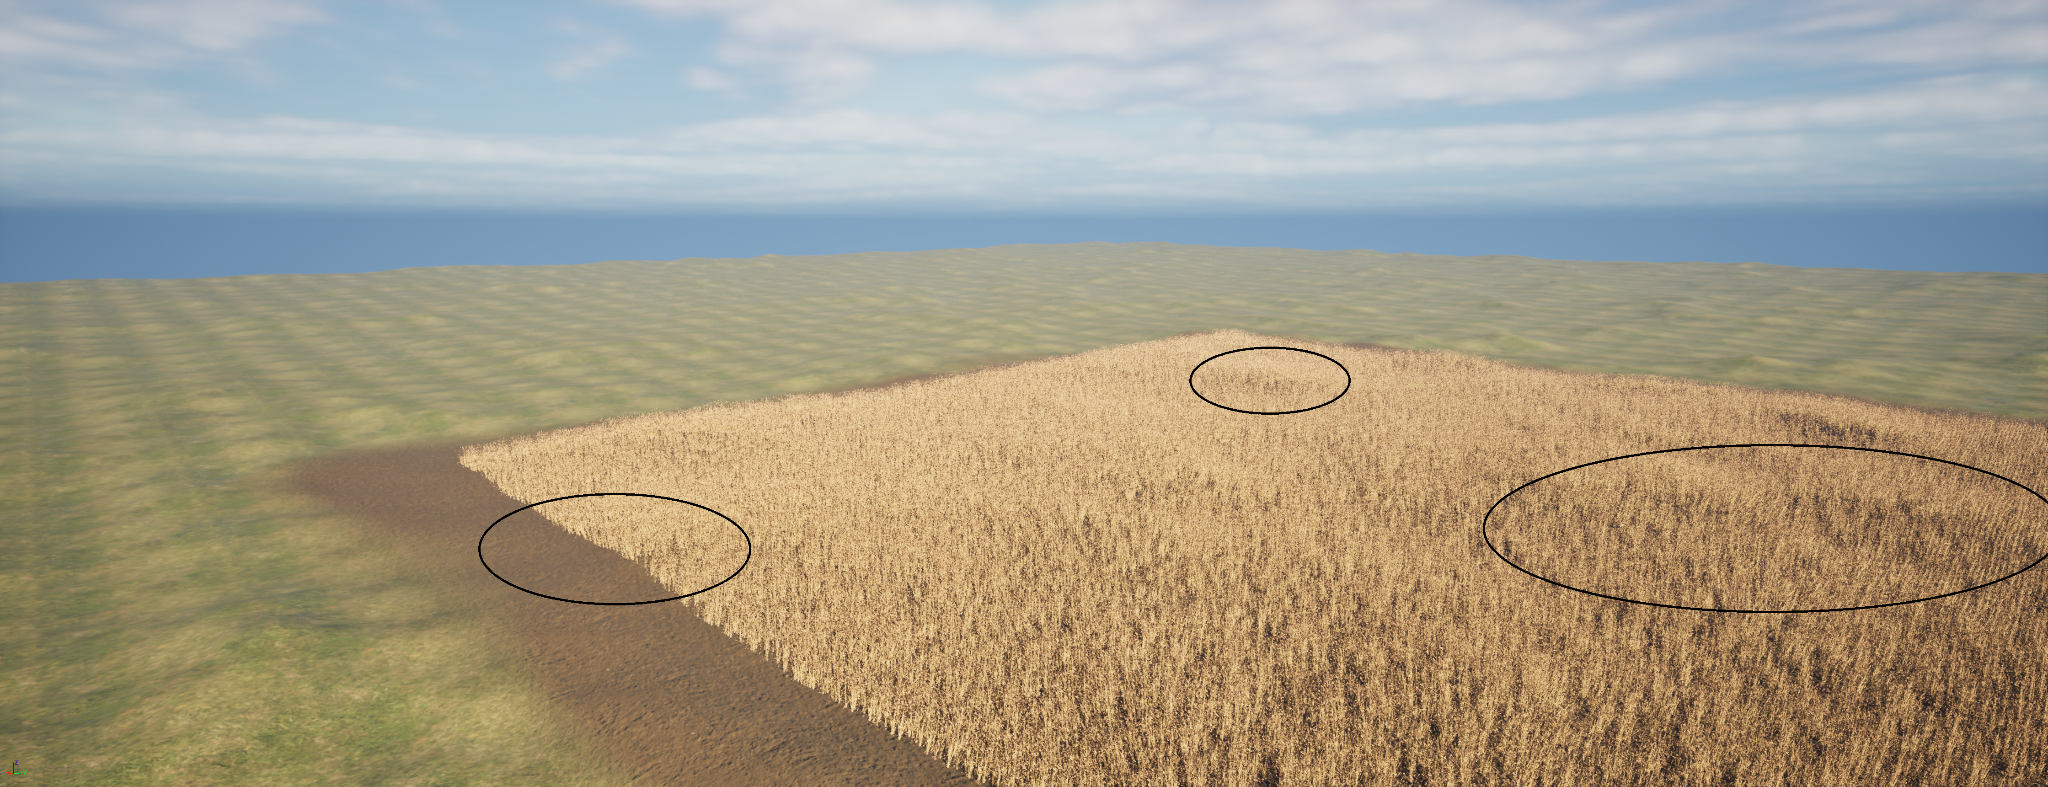
\includegraphics[width=\linewidth]{images/HighresScreenshot00002_4MB.png}
            \caption{Rendered scene with heavy terrain displacement applied. The encircled areas point out several cases of terrain curvature and its consequent effect on cast shadows upon the field canopy.}
        \end{subfigure}
        
        \caption{Using landmass to simulate terrain displacement. The "Displacement Height" parameter arranges the intensity of the terrain displacement, with  the new highest point of the terrain being half of the "Displacement Height" units above 0 and the lowest being half of the "Displacement Height" below 0.}
        \label{landmass-int}
        
    \end{minipage}
\end{figure}
    
Eventually, no data were captured with any amount of displacement, as I did not identify any efficient way for measuring illuminance in parts of the field that were shaded by the simulated short hills and valleys. However, capturing these cases remains a strong objective for the future. With the establishment of a reliable measuring method, the robustness of the trained model will be increased by their inclusion.

\subsection{Plants Generation}
The next step in the digital twin development was the generation of the crop vegetation. I selected wheat as the simulated crop species, as its dense planting structure forms a continuous canopy, suitable for observing its property of distributing reflected light unevenly. This assumption was later verified, since there were significant variations in the photometric quantities measured in the scene depending on the solar zenith angle.

The mesh I used was ”Wheat Grass” \cite{quixel_wheat_grass_fab}. I slightly adjusted its material's stock color to a warmer tone, enhancing the perceived realism of the simulation. This mesh also included a wind simulation by default, but I manually removed it to ensure that the camera captures the same scenes with each render, with the lighting conditions being the only varying factor.

\subsubsection{Procedural Content Generation}

The Procedural Content Generation (PCG) framework allows the developer to define rules for the procedural placement of assets \cite{epic_pcg_overview}. It samples the terrain and provides both the ability to place static meshes stochastically within bounds or organized in grids, with specific distances between them. I found the latter particularly useful for reducing the time needed to simulate the typical appearance of a field, since by using PCG, vegetation can be generated automatically while maintaining precision.

There were two contradicting factors affecting the organization of the meshes that represent wheat stalks. On the one hand, the plants have to be spatially organized, simulating the process of being artificially planted by specialized machinery. On the other hand, the strictly grid-based placement of wheat stalks leads to a very unnatural appearance. To tackle this, I decided that meshes would be placed on a grid, and randomness could be introduced to the scale and rotation of each mesh. Noise was also introduced to the modeled vegetation’s density, by allowing several grid cells to remain empty. The inclusion of these factors led to a sufficiently natural look.

The resulting model can be seen in Figure~\ref{pcg-field}. It can be observed that the wheat meshes are placed in an organized grid rather than completely stochastically. The introduced noise pertains to its rotation, height difference, and planting density.

\begin{figure}[htb]
    \centering
    
    \begin{subfigure}{0.48\linewidth}
        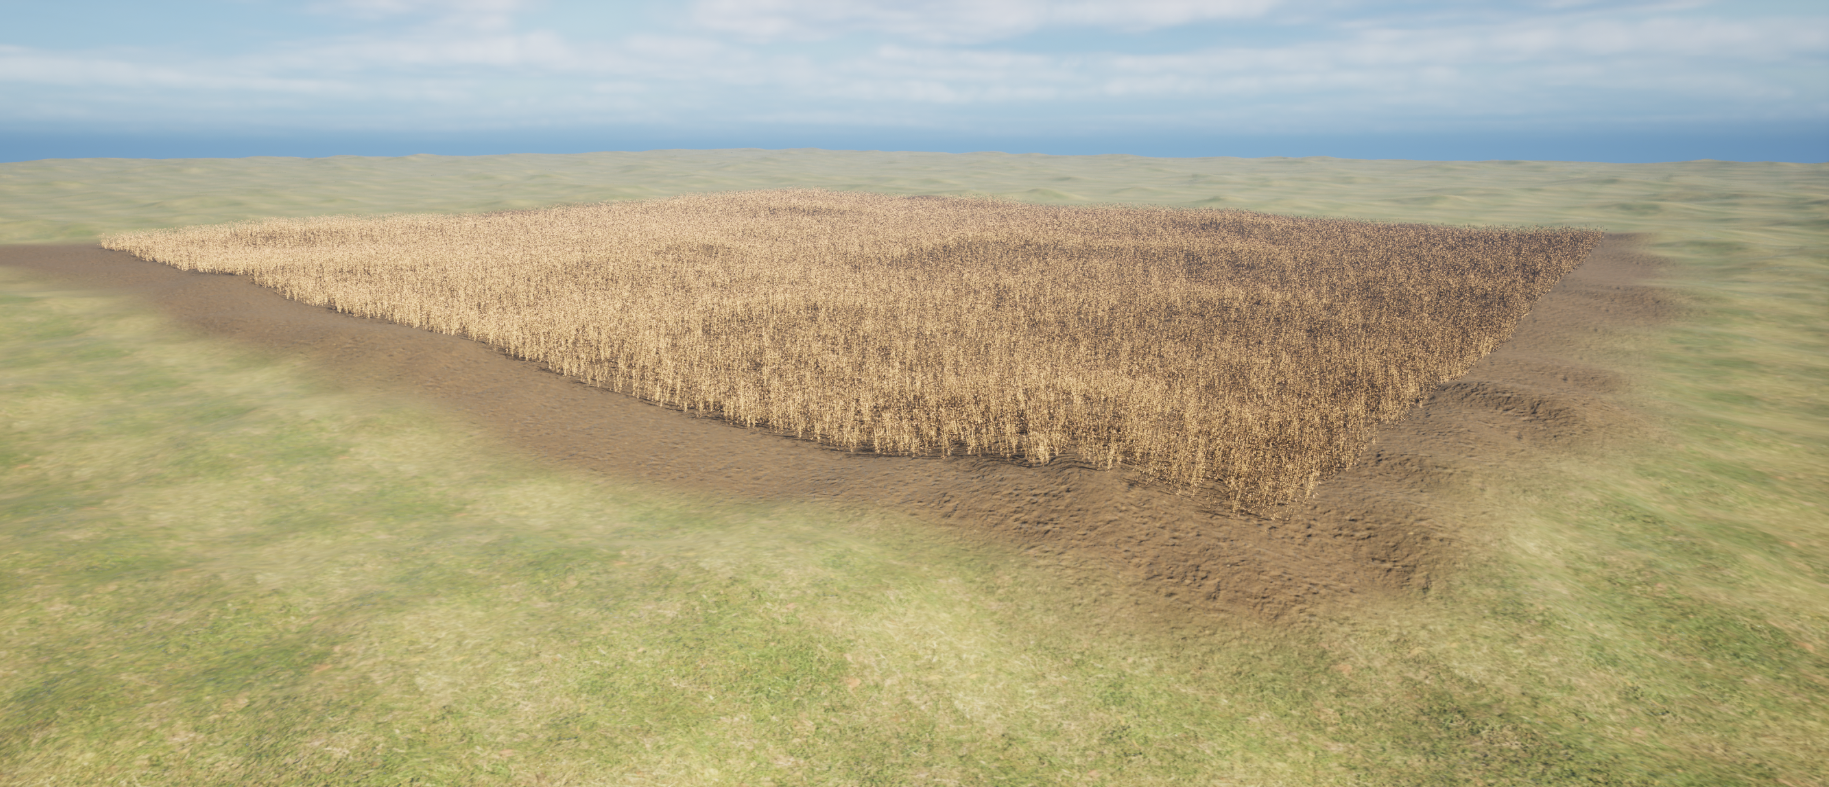
\includegraphics[width=\linewidth]{images/wheat-field.png}
        \caption{Image of the generated wheat field from the side.}
    \end{subfigure}\hfill
    \begin{subfigure}{0.48\linewidth}
        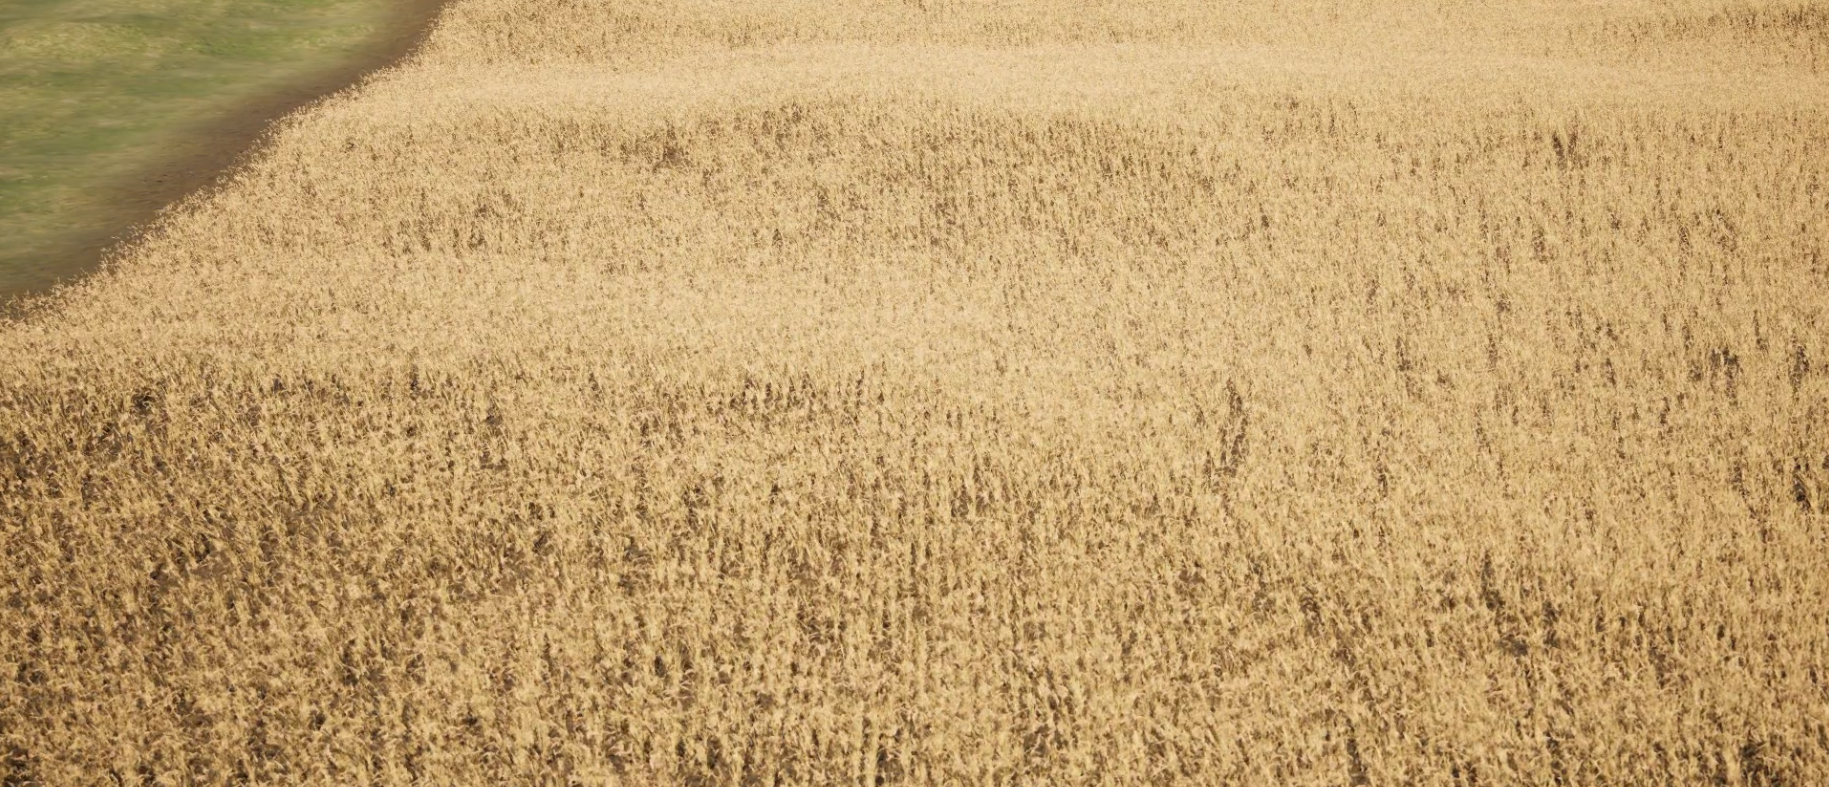
\includegraphics[width=\linewidth]{images/wheat-above.png}
        \caption{Image of the generated wheat field from above.}
    \end{subfigure}
    
    \caption{Images of wheat generated using the Procedural Content Generation tool.}
    \label{pcg-field}
\end{figure}

\subsubsection{Different Plant Materials}

So far, all the vegetation meshes inserted into the scene were sharing the same slightly altered stock material. The final part of the plants generation process was the introduction of variability to the material of the plants across the field. There were two main motives behind this addition. Firstly, this way the realism of the rendered scene is enhanced, considering that, in a real world field, the color of the crops varies due to different growth stages, hydration state, influence of a disease and more. The second motive was enlarging the diversity of the training examples. Specifically, by making the red and green band reflectance change from plant to plant in the field, the trained model becomes more robust, learning the relationships between the measured and ground truth GRVI values for more than one possible cases. It is also important to mention that, as described in more detail later on, measured GRVI appears to behave differently depending on the original GRVI of the material and the illumination conditions. This also affected the robustness of the model.

In order to simulate these differences in the reflectance of plants across the field, I developed a GRVI map, indicating the appropriate value for each part of it. To ensure a degree of realism, I used a GRVI map conceived by aerial images of an actual field (!!!!!!!!!!!!!!!! i cannot find the original publication!!!!) as the basis. Although the field studied in this work was not a wheat field, I determined that the GRVI values present in this map do appear to be realistic for lush wheat. A part of the selected GRVI map that fitted the dimensions of the simulated field was selected.

\begin{figure} [htb]
    \centering
    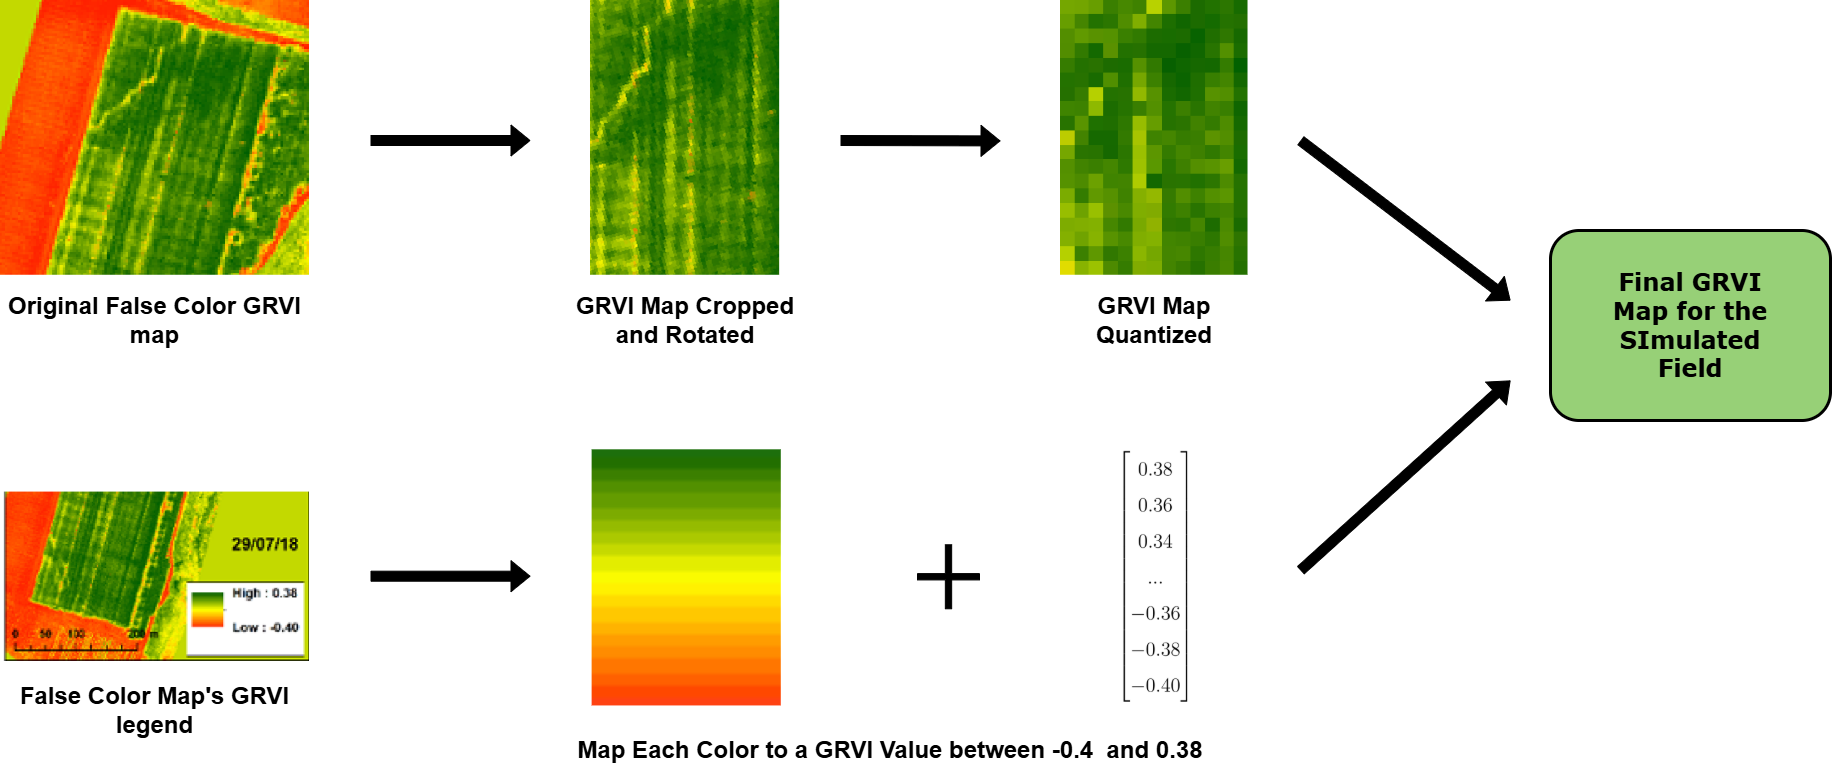
\includegraphics[width=1\linewidth]{images/grvimap.png}
    \caption{Process of creating a GRVI map for the materials assigned to the simulated field, using a real-world GRVI map as a baseline.}
    \label{grvimap}
\end{figure}

The original segment of the map was a 195 by 210 grid, with each cell representing one of 39 discrete GRVI values - identified after processing the legend of the original image. Since the reflectance assignment to the different parts of the field would have to be done either manually or the whole structure of the plant mesh generation would have to be restructured and developed as a C++ class, I avoided the exact recreation of this grid. Instead, I quantized the map using a 15 by 15 median filter, resulting in a 13 by 14 grid. Using the legend provided in the original false color map, it was possible to assign GRVI values to parts of the field based on their corresponding region in the quantized GRVI map (Figure~\ref{grvimap}). Eventually, I saved the GRVI map as a CSV file, each cell of which represented the average GRVI of the material assigned to the respective part of the field. Importantly, this is the GRVI of the material's texture, as it is applied to the meshes. When measured in the simulated environment under diffuse light conditions, due to the presence of soil and errors stemming from the calculation methods, GRVI appeared different.

Following the finalization of the GRVI map, I divided the simulated field into 1.9 by 1.9 meter segments, arranged  in the aforementioned 13 by 14 grid. Each field segment corresponded to one cell of the created CSV and was assigned the GRVI value associated with that cell. Table~\ref{tab_grvi_map} presents the GRVI values assigned to each segment, with its rows and columns corresponding to the spatial rows and columns of the simulated field, respectively. Figure~\ref{diff-griv-field} illustrates the final result of the assignment.

\begin{table}[H]
\centering
\scriptsize
\caption{Analytical table of GRVI values assigned to each part of the field.}
\label{tab_grvi_map}
\resizebox{\textwidth}{!}{%
\begin{tabular}{ccccccccccccc}
\hline
C1 & C2 & C3 & C4 & C5 & C6 & C7 & C8 & C9 & C10 & C11 & C12 & C13 \\
\hline
0.20 & 0.20 & 0.22 & 0.32 & 0.30 & 0.30 & 0.10 & 0.24 & 0.32 & 0.36 & 0.34 & 0.34 & 0.36 \\
0.22 & 0.30 & 0.34 & 0.34 & 0.28 & 0.18 & 0.30 & 0.36 & 0.38 & 0.36 & 0.36 & 0.34 & 0.36 \\
0.26 & 0.24 & 0.26 & 0.26 & 0.32 & 0.32 & 0.36 & 0.36 & 0.36 & 0.38 & 0.36 & 0.34 & 0.36 \\
0.28 & 0.32 & 0.36 & 0.26 & 0.34 & 0.34 & 0.36 & 0.36 & 0.38 & 0.38 & 0.34 & 0.26 & 0.36 \\
0.32 & 0.34 & 0.34 & 0.36 & 0.36 & 0.26 & 0.32 & 0.38 & 0.38 & 0.36 & 0.36 & 0.32 & 0.38 \\
0.34 & 0.34 & 0.36 & 0.28 & 0.36 & 0.20 & 0.30 & 0.36 & 0.38 & 0.36 & 0.32 & 0.30 & 0.36 \\
0.34 & 0.32 & 0.10 & 0.34 & 0.34 & 0.16 & 0.26 & 0.36 & 0.36 & 0.36 & 0.26 & 0.28 & 0.34 \\
0.30 & 0.30 & 0.16 & 0.36 & 0.34 & 0.32 & 0.26 & 0.34 & 0.32 & 0.34 & 0.30 & 0.32 & 0.38 \\
0.34 & 0.26 & 0.36 & 0.36 & 0.34 & 0.14 & 0.22 & 0.34 & 0.34 & 0.30 & 0.32 & 0.28 & 0.36 \\
0.08 & 0.30 & 0.36 & 0.36 & 0.32 & 0.12 & 0.30 & 0.30 & 0.32 & 0.32 & 0.26 & 0.28 & 0.36 \\
0.20 & 0.34 & 0.34 & 0.36 & 0.34 & 0.14 & 0.24 & 0.32 & 0.30 & 0.30 & 0.32 & 0.30 & 0.36 \\
0.26 & 0.30 & 0.32 & 0.30 & 0.34 & 0.14 & 0.26 & 0.34 & 0.30 & 0.26 & 0.26 & 0.22 & 0.36 \\
0.26 & 0.28 & 0.22 & 0.30 & 0.30 & 0.10 & 0.36 & 0.34 & 0.34 & 0.36 & 0.34 & 0.28 & 0.34 \\
0.20 & 0.32 & 0.24 & 0.26 & 0.30 & 0.18 & 0.16 & 0.32 & 0.28 & 0.30 & 0.26 & 0.26 & 0.34 \\
\hline
\end{tabular}%
}
\end{table}

\begin{figure} [htb]
    \centering
    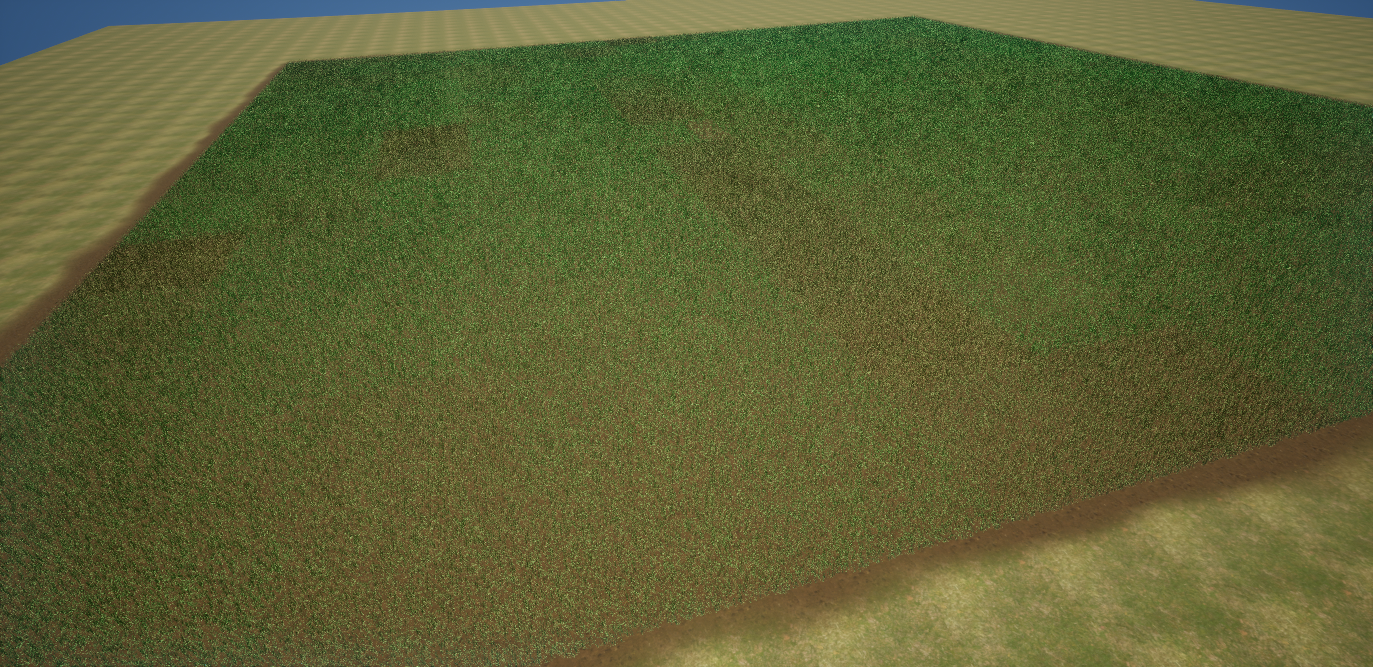
\includegraphics[width=1\linewidth]{images/HighresScreenshot00007.png}
    \caption{Digital twin after different values of inherent GRVI have been assigned to each part of the field, with each discreet segment being a 1900 by 1900 unit square.}
    \label{diff-griv-field}
\end{figure}

\subsection{Tree Meshes}

Illumination variability does not always originate solely from the position and intensity of the light source. The existence of obstacles between the light source and the studied surface do alter the illuminance reaching the surface too, and, consequently, the luminance reflected towards the sensor. Again, this would not affect the calculation of reflectance, assuming that the sensors used and the studied surface were ideal. In the studied case though, I treat shadows as one of the challenges the proposed algorithm aims to address.

An organic way to introduce shadows into the scene is to add trees to it. The objective was for the trees' crowns to cast shadows onto the simulated crops' canopy. Ideally, the created shadows do not occlude the whole field but rather parts of it. This way, by changing the solar zenith angle (SZA), the direction of the shadows changes, also changing the parts of the field that are shaded. The library of tree meshes I selected for this digital twin was \cite{european_hornbeam}. Specifically, the "FT\_EuropeanHornbeam\_Field\_02\_PP" mesh was used. Considering that only a numerable amount of meshes had to be added to achieve the desired result, and in a way that their trunks are not included in the areas of interest of the captured frames, I manually placed them using UE's Foliage Tool \cite{epicgames_foliagetool}. Figure~\ref{tsas} depicts the digital twin post the addition of tree meshes. Specifically, Figures~\ref{ts--104} and \ref{ts-104} show the difference in the shadows' directionality caused by SZA variations.

\begin{figure}[htb]
    \centering
    
    \begin{minipage}{1\textwidth}

        \begin{subfigure}{\linewidth}
            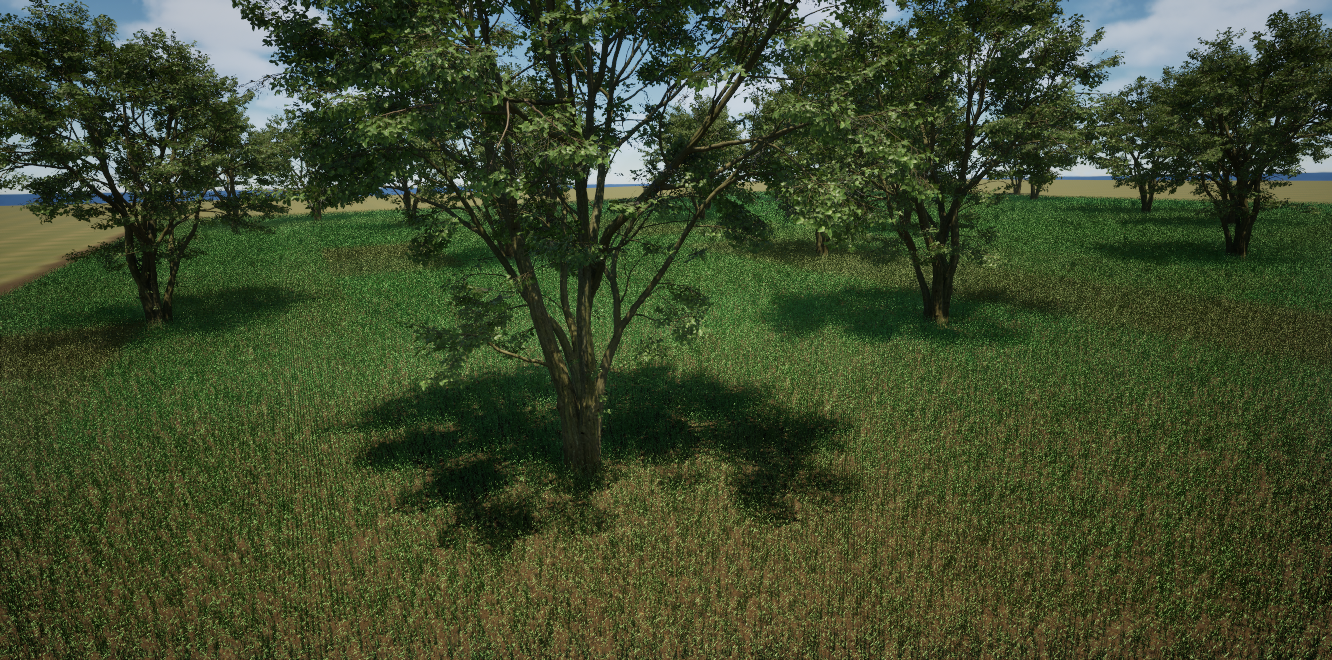
\includegraphics[width=\linewidth]{images/trees-generic.png}
            \caption{Trees added to the digital twin.}
        \end{subfigure}

        \vspace{1em}
    
        \begin{subfigure}{0.48\linewidth}
            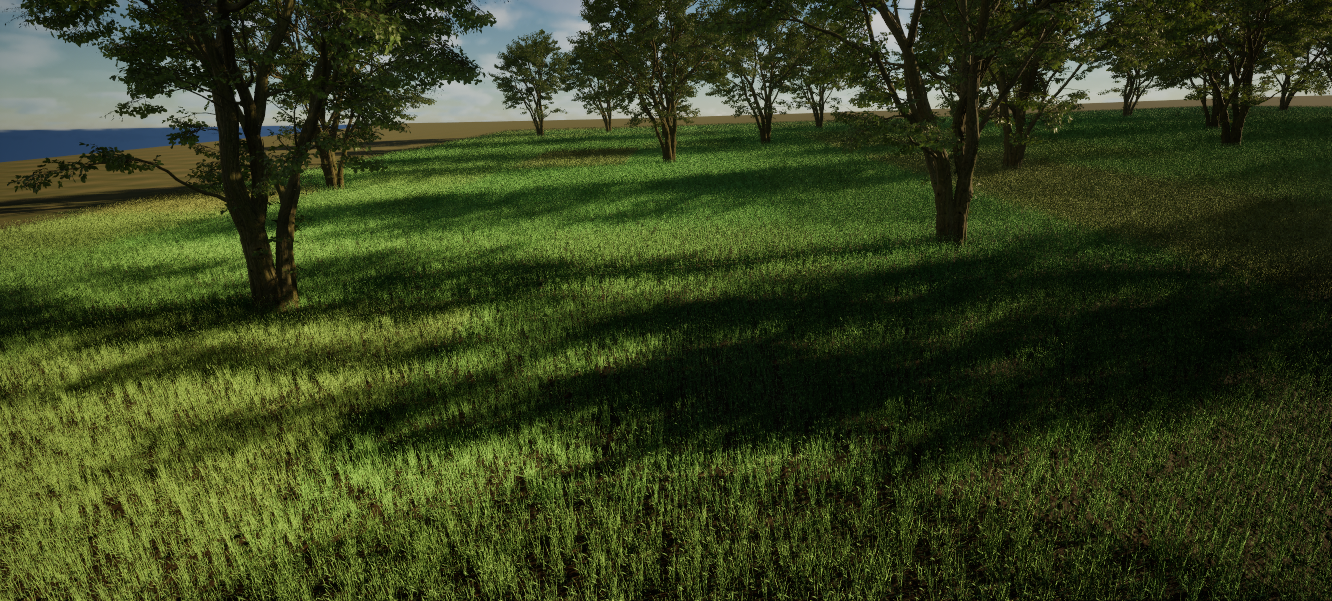
\includegraphics[width=\linewidth]{images/trees-6am.png}
            \caption{Trees' shadows for SZA $ = -104^\circ$}
            \label{ts--104}
        \end{subfigure}
        \hfill 
        \begin{subfigure}{0.48\linewidth}
            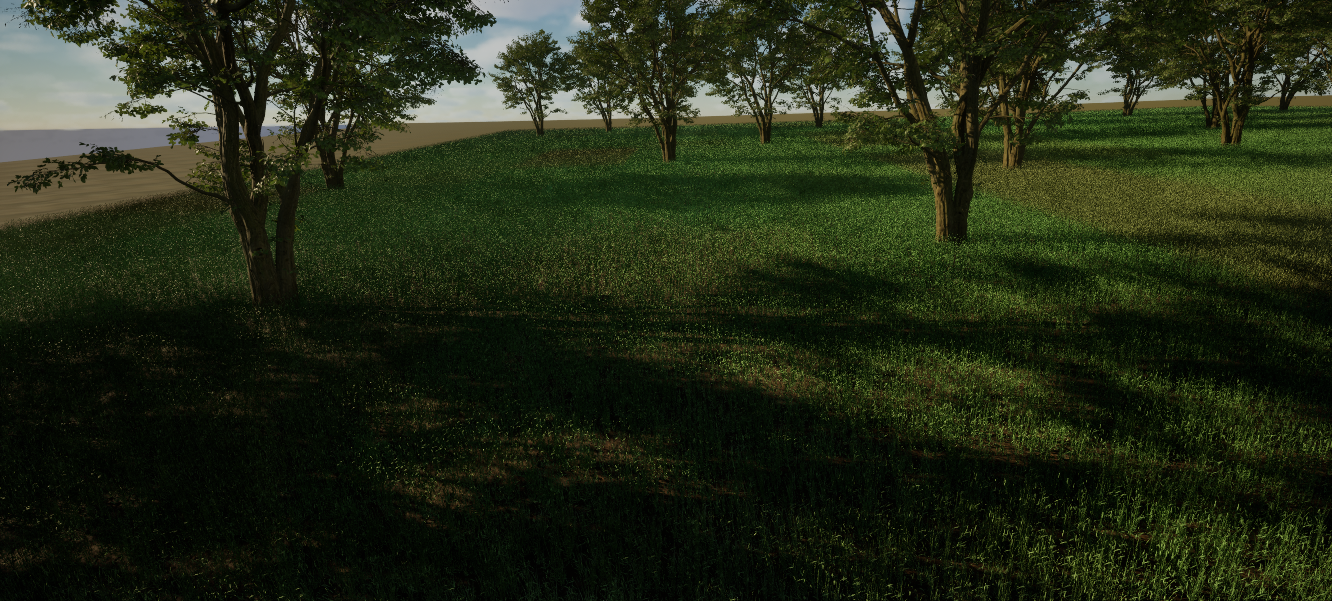
\includegraphics[width=\linewidth]{images/trees-1715.png}
            \caption{Trees' shadows for SZA $ = 104^\circ$}
            \label{ts-104}
        \end{subfigure}        

        
        \caption{Trees added to the digital twin, introducing shadows to parts of the field's canopy. The shaded parts change as the SZA changes, ensuring diversity in the training examples.}
        \label{tsas}
        
    \end{minipage}
    
\end{figure}

\subsection{Lighting Configuration}

The main lighting actors in UE are:

\begin{itemize}
    \item \textbf{Point Light}: Light source similar to a light bulb
    \item \textbf{Spot Light}: Projects light in a cone shape, like a spotlight
    \item \textbf{Rect Light}: Similar to photography umbrellas. Projects light in a cone and creates soft shadows 
    \item \textbf{Directional Light}: Mimics sunlight. Illuminates the whole scene, but its direction determines the behavior of the shadows.
    \item \textbf{Sky Light}: Applies ambient lighting to the scene. Good for simulating outdoor lighting conditions
\end{itemize}

The implemented model contains the last two options, as they are directly suitable for simulating weather phenomena. Directional Light is essential in scenes where the sky is clear, controlling the direction of incident solar radiation and the resulting shadows, while Sky Light is more prominent in scenes with diffuse lighting, where radiative flux is assumed to be incident more uniformly across the scene.

In order to achieve further precision, I manipulated the parameters of Directional Light through the "Sun Position Calculator" plugin. "Sun Position Calculator" can be used for setting the appropriate roll, pitch, and yaw values of the light source, corresponding to the solar position for a specified time and set of geographical coordinates. As a result, the simulated lighting conditions can be more realistic than if the degrees were adjusted manually. The plugin also allows adjustments to the Directional Light intensity, enabling the simulation of brighter and darker scenes.


\subsection{Weather Phenomena Simulation}

There were mainly two sky conditions relevant to this study: clear-sky and cloudy-sky. Clear-sky weather represents the challenging case since, as mentioned above, the position of the sun affects the way radiation is reflected by vegetation. I constructed the simulation in a way that allows multiple Directional Light configurations, considering that there was an apparent need for data collected under more than one illumination scenario in order to achieve higher model robustness. The data collected under these various clear-sky illumination configurations later served as the model's inputs and resemble GRVI values calculated with a high degree of error. In contrast, cloudy-sky weather is treated as ideal for the collection of the ground truth data, since the luminance measured in such conditions remains sufficiently invariant for various solar coordinates.

Clear-sky conditions were easier to implement, given that the default configuration of Sun Position Calculator already does simulate this weather state. Optionally, the Volumetric Clouds actor, which can also be included by default during the creation of a new level in Unreal Engine, can be disabled to fully simulate clear sky. However, this actor itself does not affect Directional Light significantly, as it does not cause light scattering or cast additional shadows.

The primary tool I used for replicating cloudy-sky conditions is “Sky Atmosphere”. In Unreal Engine 5, Sky Atmosphere is a system used for the simulation of the atmosphere of a planet. Among the available options, there are parameters for adjusting the atmospheric height and color and, most importantly for this task, the amount of light diffusion and absorption occurring as sunlight enters the atmosphere and comes in contact with its particles. These parameters are named ”Mie Scattering Scale” and ”Mie Absorption Scale”, respectively. In the context of this work, I focused more on experimenting with "Mie Scattering Scale" adjustments, as the objective was to identify a configuration that eliminates the directionality of light without reducing the brightness of the scene. Ultimately, by increasing the intensity of Directional Light and Mie Scattering Scale and decreasing the amount of light absorption, a desirable result was achieved.

Figure~\ref{notclvscl} illustrates the difference between zero and non-zero Mie Scattering Scale applied. In the first case (Figure~\ref{nonfog}), the solar zenith angle (SZA) is set to $56^o$, making the sun closer to the right side of the frame. Consequently, the rightmost half of the field appears less illuminated than the leftmost. When cloudy weather is simulated, though (Figure~\ref{fog}), despite the SZA remaining the same, the illumination unevenness gets mitigated.
 
\begin{figure}[htb]
    \centering
    
    \begin{subfigure}{0.48\linewidth}
        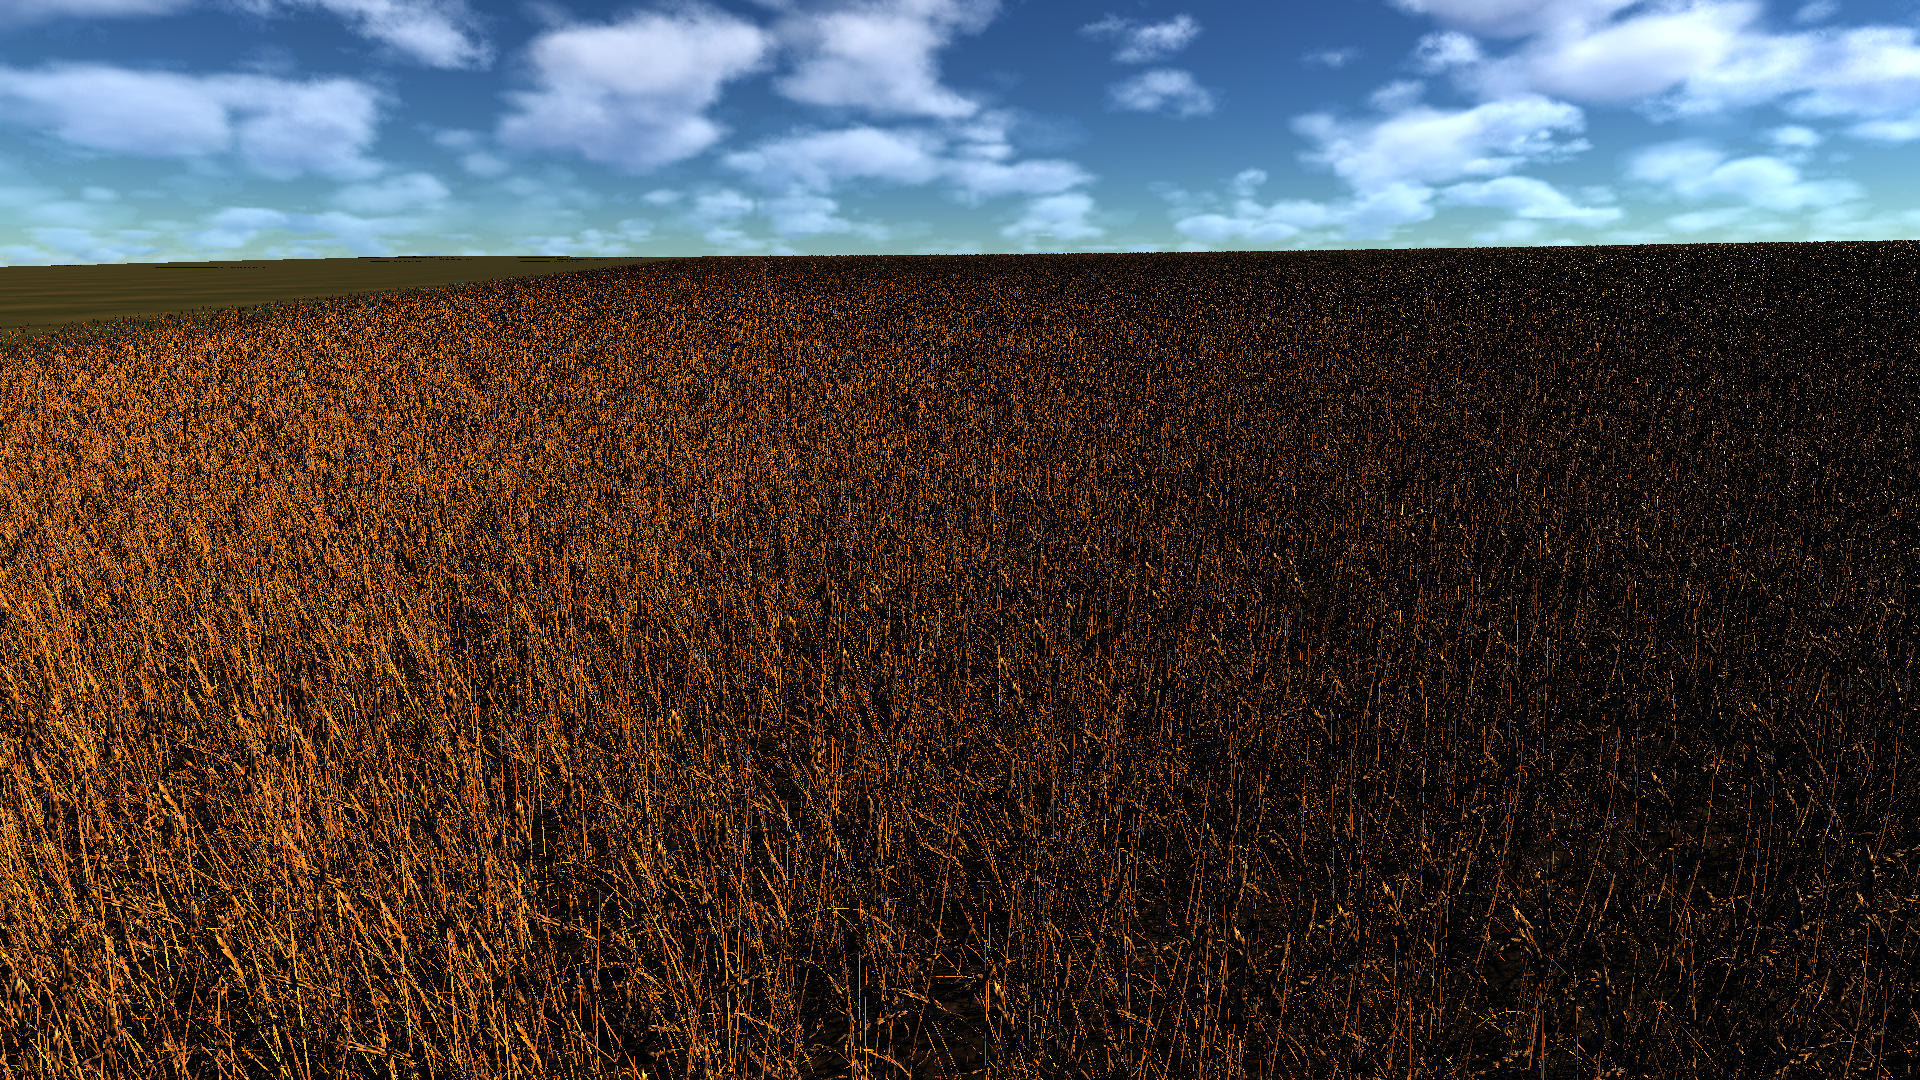
\includegraphics[width=\linewidth]{images/nonfoggy10.png}
        \caption{Field illuminated with the SZA being set to $56^o$ and Mie Scattering Scale being set to its default value (near zero).}
        \label{nonfog}
    \end{subfigure}\hfill
    \begin{subfigure}{0.48\linewidth}
        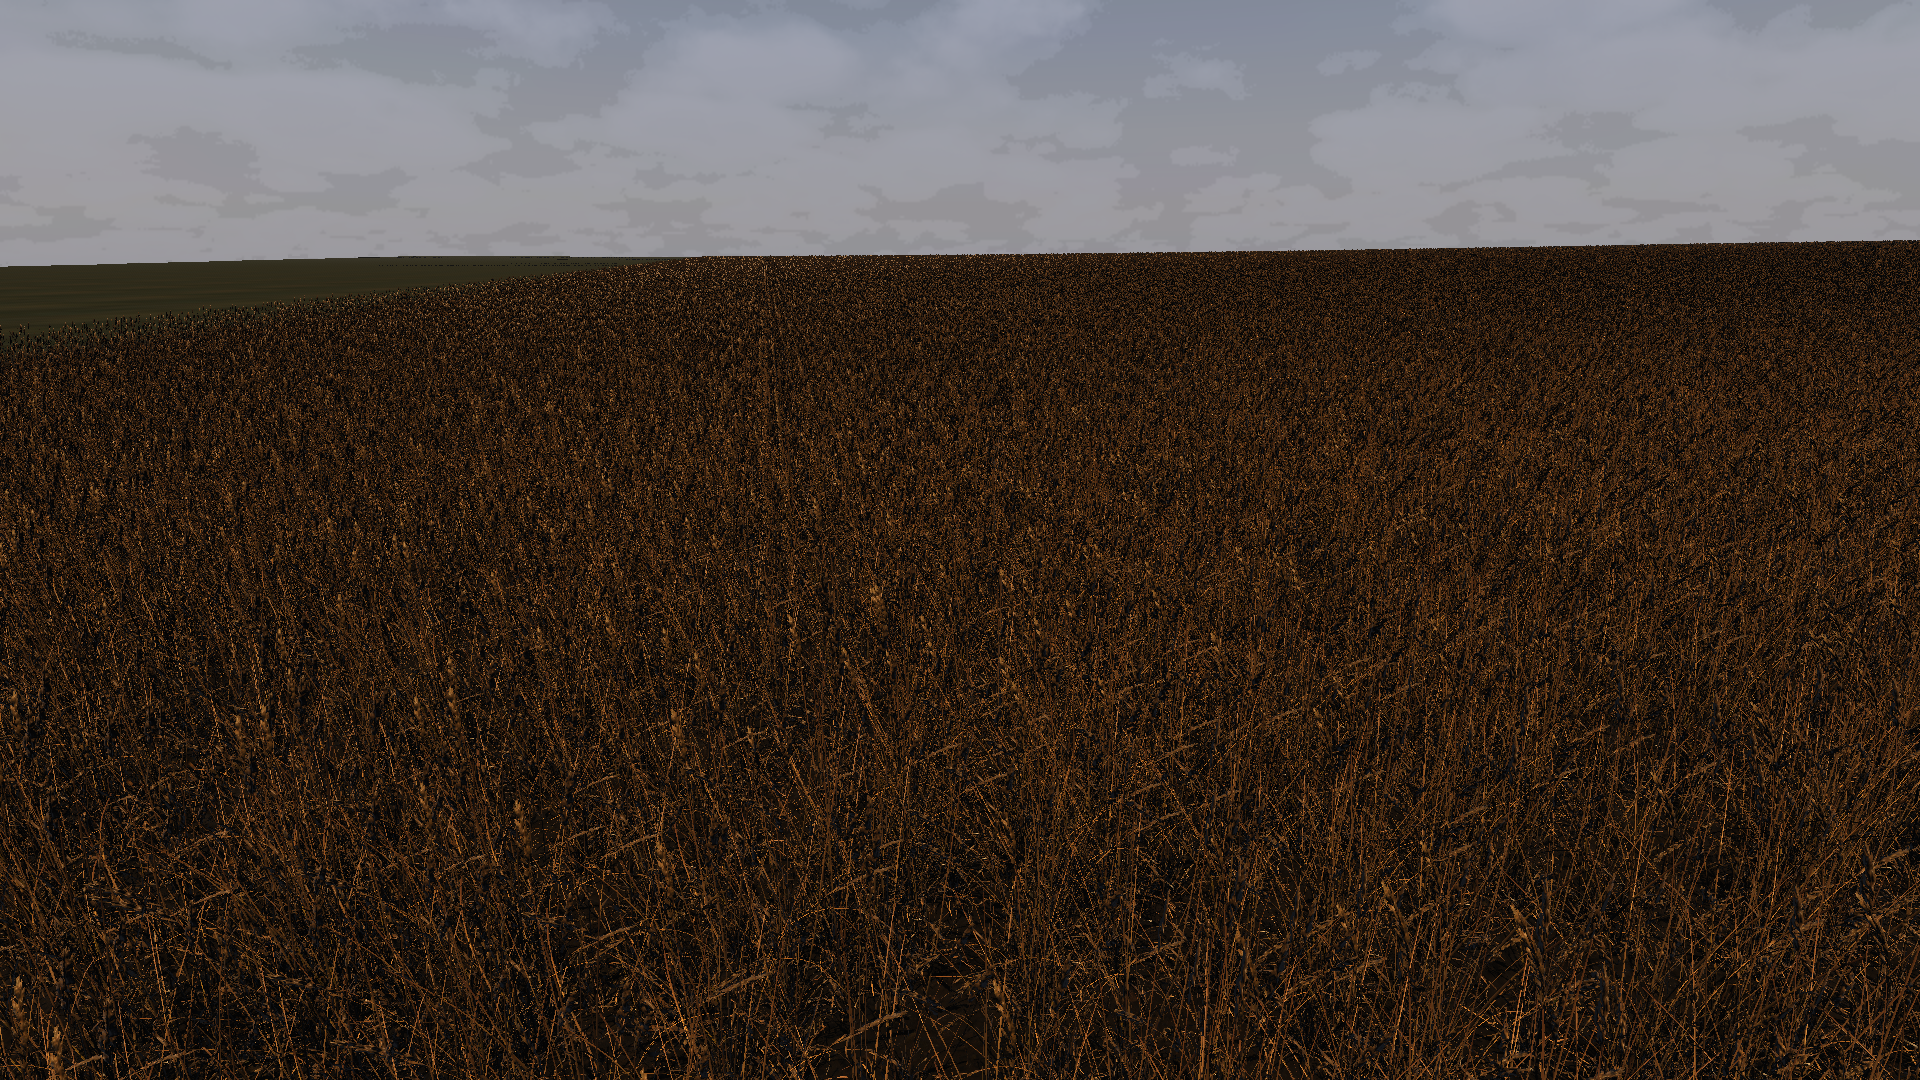
\includegraphics[width=\linewidth]{images/foggy10.png}
        \caption{Field illuminated with the SZA being set to $56^o$ and Mie Scattering Scale being increased to a non-zero value.}
        \label{fog}
    \end{subfigure}
    
    \caption{Images captured using the same SZA and different Mie Scattering Scale values. As the latter increases, simulating cloudy weather, the effects of the wheat canopy's anisotropic BRDF are mitigated, making the field appear evenly illuminated.}
    \label{notclvscl}
\end{figure}

\section{Photometric Quantities Measurement}
\label{photom-q-meas}

For the calculation of GRVI, the reflectance of a surface for the green and red bands should be calculated beforehand. As an approximation, I decided to use the reflectance formula for Lambertian surfaces in order to simplify this process. Although this contradicts the previously stated fact that a wheat field's canopy behaves as an anisotropic reflector, the error introduced during the calculation of reflectance is included in the challenges the trained models aim to address. The formula for calculating the reflectance of an ideal surface per band is:

\begin{equation}
    \rho_b = \frac{L_b \times \pi}{E_b}
    \label{lambertian}
\end{equation}

where $\rho_b$, $L_b$ and $E_b$ are the reflectance per band (dimensionless), luminance per band in nits and illuminance per band in lux, respectively. Clearly, the first step of approximating the GRVI of a studied surface was identifying consistent ways for acquiring the illuminance and luminance information from the synthetic scene.

\subsection{Acquiring Illuminance}

Illuminance is the amount of luminous flux falling onto a surface per unit area. Illuminance is commonly measured in lux. It is also measured in lux in this study, as that favors the calculation of reflectance.

In real-world applications, illuminance is usually measured using a lux meter, a type of light meter. This inspired me to use a virtual light meter within the digital twin. After finding an already developed implementation of a custom virtual light meter \cite{weiss_2025_lightmeter}, I added it to the project as a plugin and used it for approximating illuminance at every point of interest in the field.

The way this light meter works is by using an UE's Scene Capture Component actor to render radiometric linear images of a white surface, calculating the luminance of the light reflected by the surface using pixel values and, through it, calculating illuminance. A variable of the light meter actor stores the measurement. Initially, the light meter could only calculate the combined illuminance of all three channels. I modified its Blueprint to overcome this limitation and expose the illuminance of the green and red bands separately.

The placement of the light meter in the digital environment and the method employed for retaining its readings is analyzed later on.

\subsection{Acquiring Luminance} \label{findlum}

Luminance is the measure of the amount of light reflected by a surface and perceived by a sensor. In order for this information to be extracted from an Unreal Engine environment, a deeper understanding of the Unreal Engine's color rendering pipeline should be achieved.

The Unreal Engine’s color rendering pipeline, as described in UE’s documentation \cite{oztalay_2021_colorpipeline}, is displayed in Figure~\ref{cl-pp}. The first part of the pipeline is the description of the textures appearing in the scene, many of which are in the 8-bit, sRGB color space. These textures are then converted to the engine’s linear working space and, after they interact with the scene’s lighting and shading, an HDR image is produced. This is what UE’s tools refer to as Scene Color, and it expresses the rendered luminance before any kind of post-processing is applied.

\begin{figure} [htb]
    \centering
    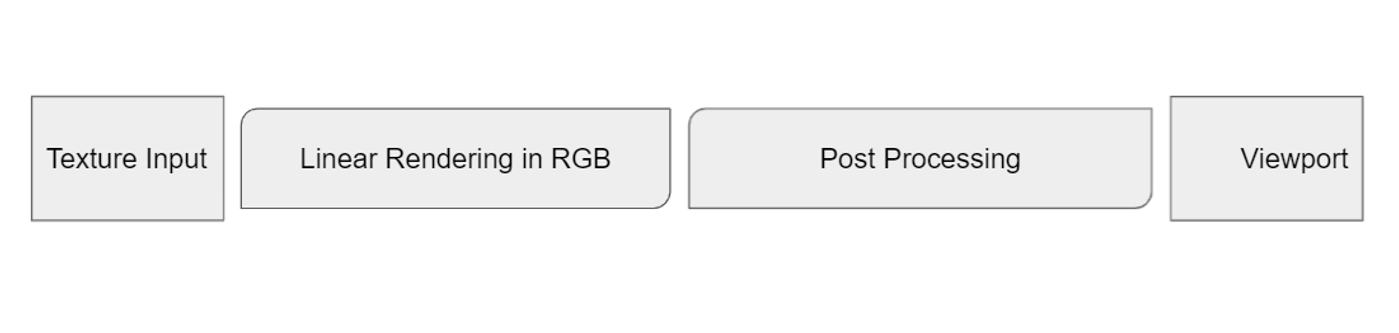
\includegraphics[width=1\linewidth]{images/color_pipe.png}
    \caption{Unreal Engine's color rendering pipeline.}
    \label{cl-pp}
\end{figure}

Post-processing includes several steps, and it is responsible for the transformation of the pixel values rendered in Scene Color to the values that appear in the viewport. The steps that are considered more relevant in the context of this study are the ones that affect the luminance as it is perceived by a sensor, and they are managed by Tonemapper. Tonemapper is a non-linear system responsible for mapping the Scene Color to a dynamic range that can be displayed to the editor’s viewport, while also applying lighting-relevant adjustments like bloom and exposure. Although tonemapping was overall observed to produce more realistic colors, compared to the ones appearing in raw Scene Color, its black-box nature affects the usability of the produced image. More importantly, the illuminance estimated from the Scene Color values, as described before, is more strongly associated with the luminance derived from Scene Color than with the color values displayed in the viewport.

For the scene luminance to be captured, an equivalent to the Cine Camera actor should be identified, capable of capturing the colors as they appear in the scene. The actor with the closest functionality to this is the Scene Capture Component (SCC) 2D. By setting SCC to capture the linear scene color, it is possible to see the pre-tonemapping colors, which are equivalent to luminance. A drawback of SCC is that it does not provide a straightforward way to save the captured images to the computer's disk, at least in an automated way. Unreal Engine does allow the user to save the captured images of the scene manually in .EXR format, with pixels representing linear luminance values, but saving images one by one is not viable. To overcome this challenge, I used an already existing actor class called Frame Capture Manager, the source code for which I found online \cite{hess_unrealimagecapture}. Its main functionality is to expose the aforementioned feature of UE that allows the user to manually save the images captured by SCC to other actors in the form of a function (void CaptureNonBlocking()), enabling the automated capturing and saving to disk of scene color images. More about the Frame Capture Manager and how it was used in this context is explained in the \hyperref[chap4]{Data Collection} chapter.

\begin{figure}[htb]
    \centering
    
    \begin{subfigure}{0.48\linewidth}
        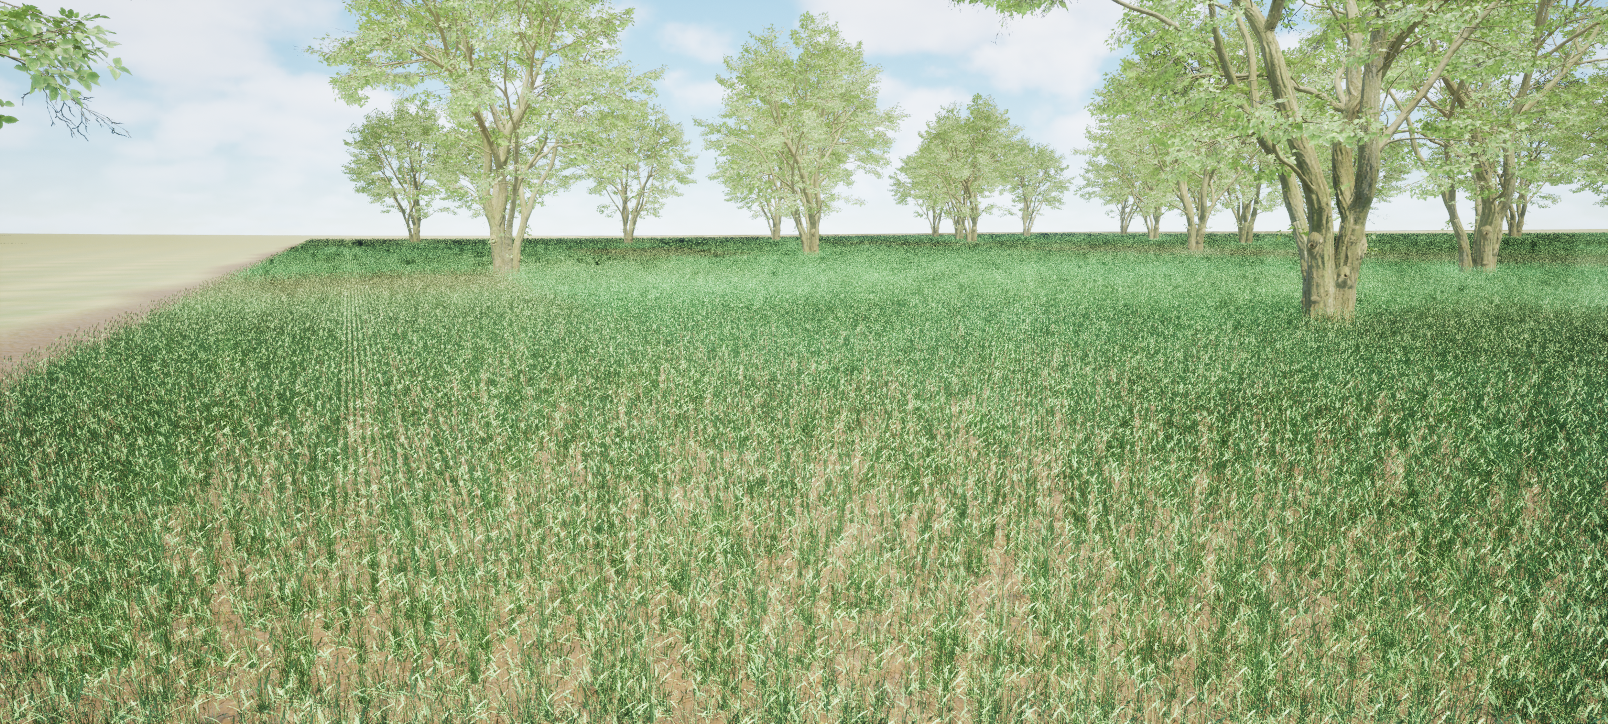
\includegraphics[width=\linewidth]{images/viewport_img.png}
        \caption{Image captured as rendered in the viewport.}
        \label{viewport}
    \end{subfigure}\hfill
    \begin{subfigure}{0.48\linewidth}
        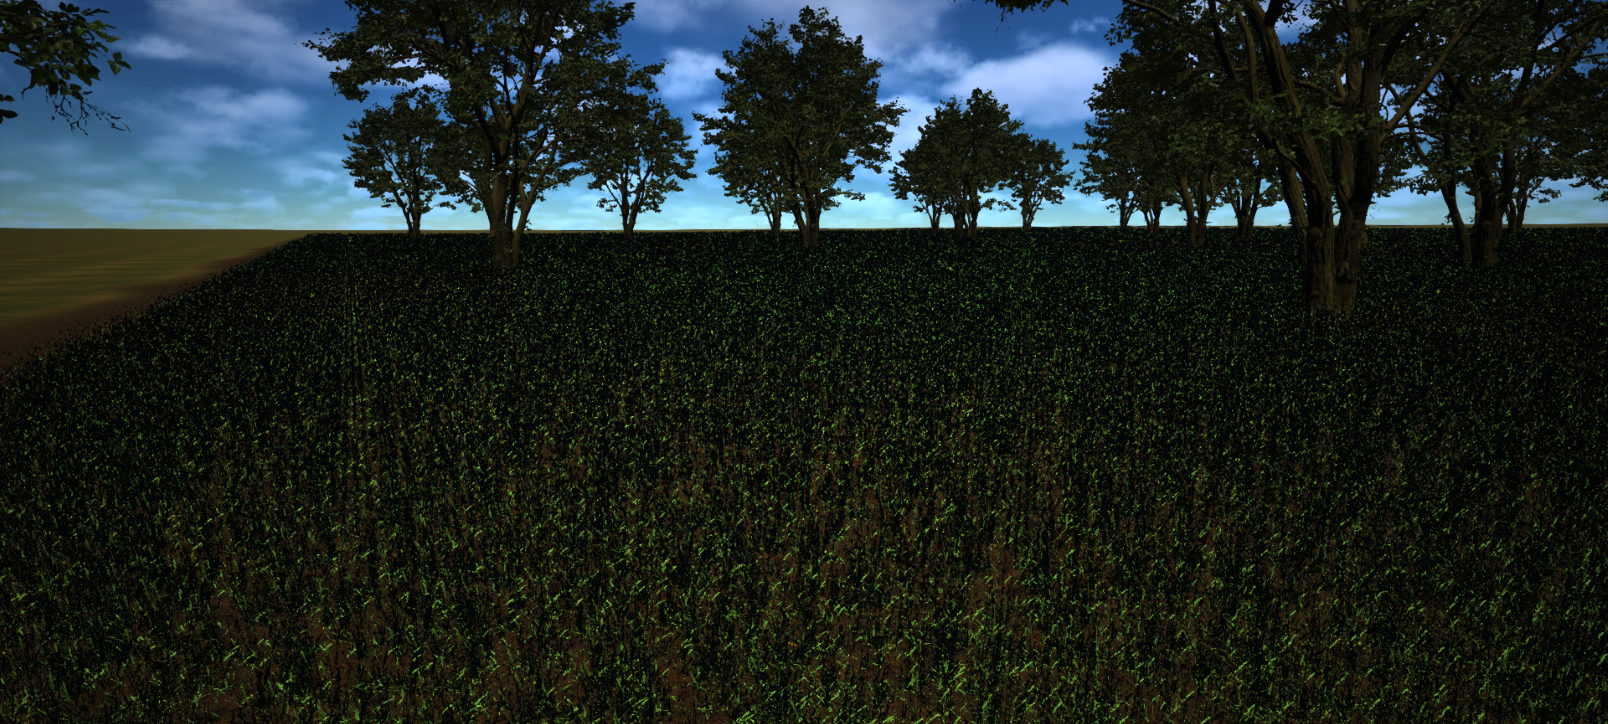
\includegraphics[width=\linewidth]{images/scc_img.png}
        \caption{Image captured using SCC.}
        \label{scc}
    \end{subfigure}
\end{figure}
    \chapter{Data Collection}
\label{chap5}

After completing the implementation of the digital environment, the next step was preparing the data needed for the training of the machine learning models. This process was separated into four main parts:

\begin{itemize}
    \item \textbf{Deciding} which illumination scenarios will be included in the dataset and how many frames will be captured per scenario (Section~\ref{illum-scenarios-sec}).
    \item \textbf{Collecting the data}, using the tools provided by UE (Section~\ref{DC}).
    \item \textbf{Assessing their quality}, ensuring that the inputs do appear influenced by the sources of error discussed in \hyperref[chap1]{the Introduction} (Section~\ref{datasssessment}).
    \item \textbf{Preprocessing them}, both by structuring them in a format compatible with machine learning frameworks and libraries, and by applying feature engineering methods (Chapter~\ref{chap6}).
\end{itemize}

Together, these four stages formed the data preparation pipeline, ensuring that the resulting dataset was sufficiently diverse, representative of the conditions under investigation, and suitable for training the selected machine learning models. The following sections describe in detail the methods employed for acquiring the raw data, while their preprocessing is discussed in the next chapter.

\section{Illumination Scenarios and Data Collection Preparation}

\label{illum-scenarios-sec}

The pivotal point for all the separate illumination scenarios was the value of green-band illuminance, as it was measured at a point of the field that is not affected by the shadow of a tree. The reasoning behind this selection is that illuminance dictates the brightness of the scene. Training a machine learning model for substantial differences in how bright the frames appear was expected to make it more robust. Additionally, the ultimate goal is to measure how much of this incident radiation is reflected towards the sensor, meaning that having controlled green- and red-band illuminance values would assist with this purpose. I selected four discreet green-band illuminance values: 200, 322, 480 and 1020, scaling from barely visible scene to nearly overexposed, resulting in four separate illumination groups.

Since UE's environment mimics several real-world phenomena, including the interactions between the sun's light and Earth's surface and atmosphere, the value of illuminance measured at the surface of a level is dictated by three parameters: solar zenith angle, Mie Scattering Scale and Directional Light intensity. If both the value of Mie Scattering Scale and solar zenith angle (SZA) are set to zero, the combined measured illuminance is close to the intensity of of the Directional Light. If the absolute value of at least one of the two is increased, less radiant flux reaches the surface, resulting in smaller values read by the light meter. To compensate for that and retain the same green-band illuminance value across each illuminance group, the Directional Light's intensity increases as the absolute value of the SZA or Mie Scattering Scale increases. 

The intensity of the incident radiation is not the only thing that changes as the absolute SZA increases. Along with it, the analogy of red- and green- band illuminance in each angle also changes, with the higher absolute SZA values tending to result in higher $R_{RG = }\frac{E_R}{E_G}$ ratio, where $E_R$ and $E_G$ are the red- and green-band illuminance respectively. For this reason, it was particularly interesting to collect data under various SZA values, examining how this difference in $R_{RG}$ affects the perceived GRVI. I captured Data for a total of seven distinct SZA values within each illuminance group, including three pairs of angles equal in magnitude but opposite in sign and the angle $20^\circ$, as it lead to the $R_{RG}$ closest to one. The result was $7 \times 4 = 28$ different illumination scenarios. The parameters defining each illumination scenario scenario are presented in Table~\ref{ilmsce}.

I decided to perform two render sequences for each illumination scenario: one where the camera starts at the beginning of the spline and ends at the end of the spline, and one that follows the exact opposite direction. Additionally, for all the $28 \times 2 = 56$ cases, the exact same were to be performed, this time with the inclusion of trees, in order to introduce shadows, totaling at 112 discreet render sequences. Each render sequence is consisted of 298 frames (300 frames in total, with two warm-up frames that were deleted in preprocessing and 298 actually usable frames), with the exception of few cases where one or two frames did not have matching light meter data, and their inclusion was avoided. This lead to a total of approximately 33376 frames. I eventually planned to construct two versions of the dataset, one deriving from the whole set of frames that were captured and one from the half that did not include trees, aiming to assess the models' predictive ability with different sources of error present. In addition, two further datasets were to be generated, again, one with trees present and one without, this time with the ground truth value being the materials' inherent GRVI.

\section{Data Collection}
\label{DC}

The largest proportion of the research effort for this work was allocated to identifying reliable ways for collecting data within the digital environment and storing them in an organized manner. In total, approximately 33376 EXR images were captured, the values of which represent the luminance of the scene as perceived by the sensor's lens. All frames are accompanied with a detailed context over the relevant environmental and actor parameters present during the rendering of the shot, including:
\begin{itemize}
    \item the coordinates and rotation angles of the sensor
    \item the rotations angles of Directional Light (sun)
    \item the light meters' readings
    
\end{itemize}

From each captured image, only several segments were retained as areas-of-interest. Each image contains 20 areas-of-interest, meaning that the complete version of the dataset is consisted of approximately 667520 samples.

\subsection{Camera Splines}

The first step in capturing the training data was defining the route the Scene Capture Component (SCC) actor would have to follow, rendering linear images of the scene in the process. I developed a C++ actor class that, given the dimensions of the field and its coordinates in the world, automatically creates a sequence of spline points, shaping an orthogonal polyline. The spline points project onto the Landscape actor and are then offset by a fixed number of units, ensuring that if terrain displacement is applied, the route will follow its trend (Figure~\ref{spline}).

\begin{table}[H]
\centering
\begin{tabular}{|c|c|c|c|}
\hline

\textbf{SZA} &
\textbf{Source Intensity} &
\textbf{Green-Band Illuminance} &
\textbf{Red-Band Illuminance} \\

\hline

\multirow{4}{*}{-104}
&1120 & 200  & 262,126637\\ \cline{2-4}
& 1800& 322  & 420,973416 \\  \cline{2-4}
&2684 & 480  &  627,925832\\ \cline{2-4}
&5700 & 1020 &  1334,39148\\ \hline

\multirow{4}{*}{-85}
&406 & 200  & 229,336264 \\ \cline{2-4}
& 655& 322  & 370,118885 \\ \cline{2-4}
&975 & 480  &  550,956812\\ \cline{2-4}
&2070 & 1020 & 1169,457865\\ \hline

\multirow{4}{*}{-56}
&273 & 200  & 222,26768\\ \cline{2-4}
&439 & 322  &357,356164 \\ \cline{2-4}
&654 & 480  &532,499955 \\ \cline{2-4}
& 1389& 1020 &1130,973355 \\ \hline

\multirow{4}{*}{20}
&252 & 200  &220,893233 \\ \cline{2-4}
&405 & 322  &355,589018 \\ \cline{2-4}
& 604& 480  &529,358362 \\ \cline{2-4}
&1283 & 1020 &1124,69017 \\ \hline

\multirow{4}{*}{56}
&273 & 200  &221,874981 \\ \cline{2-4}
&439 & 322  & 356,963465 \\ \cline{2-4}
&654 & 480  & 531,714557\\ \cline{2-4}
&1389 & 1020 & 1129,402559\\ \hline

\multirow{4}{*}{85}
& 406 & 200  &228,550866 \\  \cline{2-4}
& 655& 322  &368,744438 \\ \cline{2-4}
&975 & 480  &548,600617 \\ \cline{2-4}
& 2070& 1020 &1165,530874 \\ \hline

\multirow{4}{*}{104}
& 1120 & 200  & 262,715686 \\\cline{2-4}
&1800 & 322  &422,151513 \\ \cline{2-4}
&2684 & 480  & 629,496628\\ \cline{2-4}
&5700 & 1020 &  1336,747674\\ \hline

\multirow{4}{*}{GT}
& -  & 200  & - \\ \cline{2-4}
& -& 322  &- \\ \cline{2-4}
& -& 480  &- \\ \cline{2-4}
&2985 & 1020 &1123,904772 \\ \hline

\end{tabular}
\caption{Table presenting illuminance per band per SZA. GT represents cloudy weather.}
\label{ilmsce}

\end{table}

\begin{figure}[htb]
    \centering
    
    \begin{subfigure}{0.48\linewidth}
        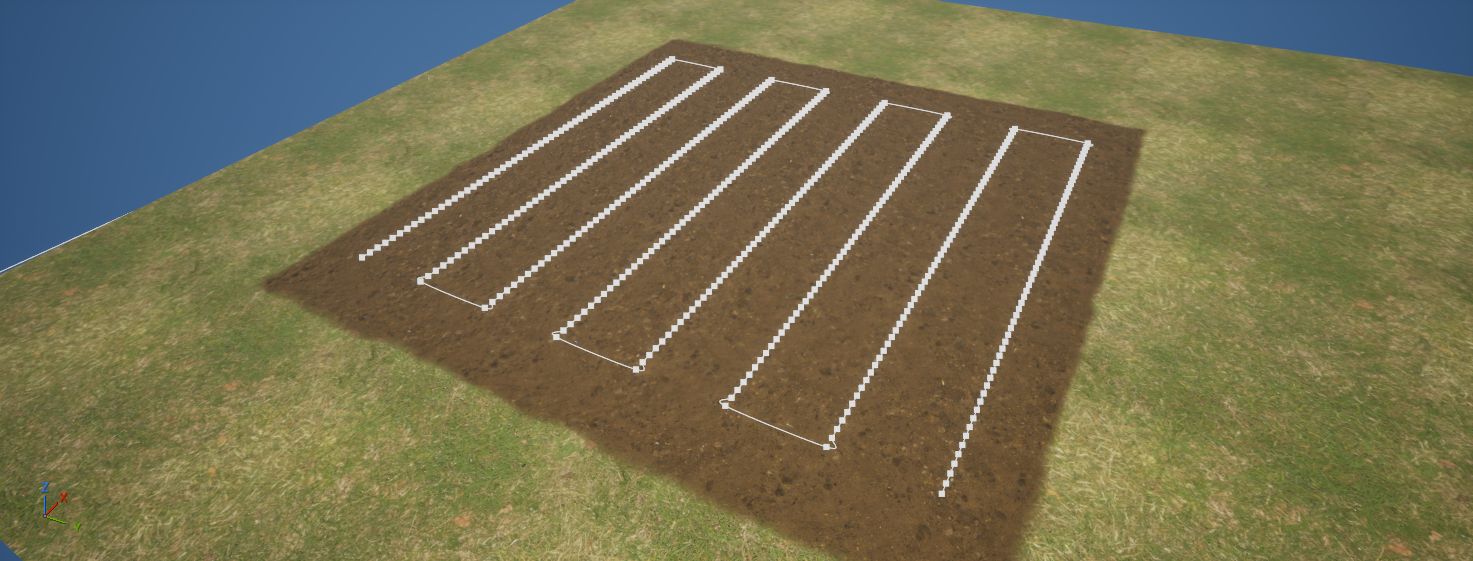
\includegraphics[width=\linewidth]{images/spline_polyline.png}
        \caption{The complete route, defined by individual spline points. The sensor follows this route while capturing images of the scene.}
        \label{splpoly}
    \end{subfigure}\hfill
    \begin{subfigure}{0.48\linewidth}
        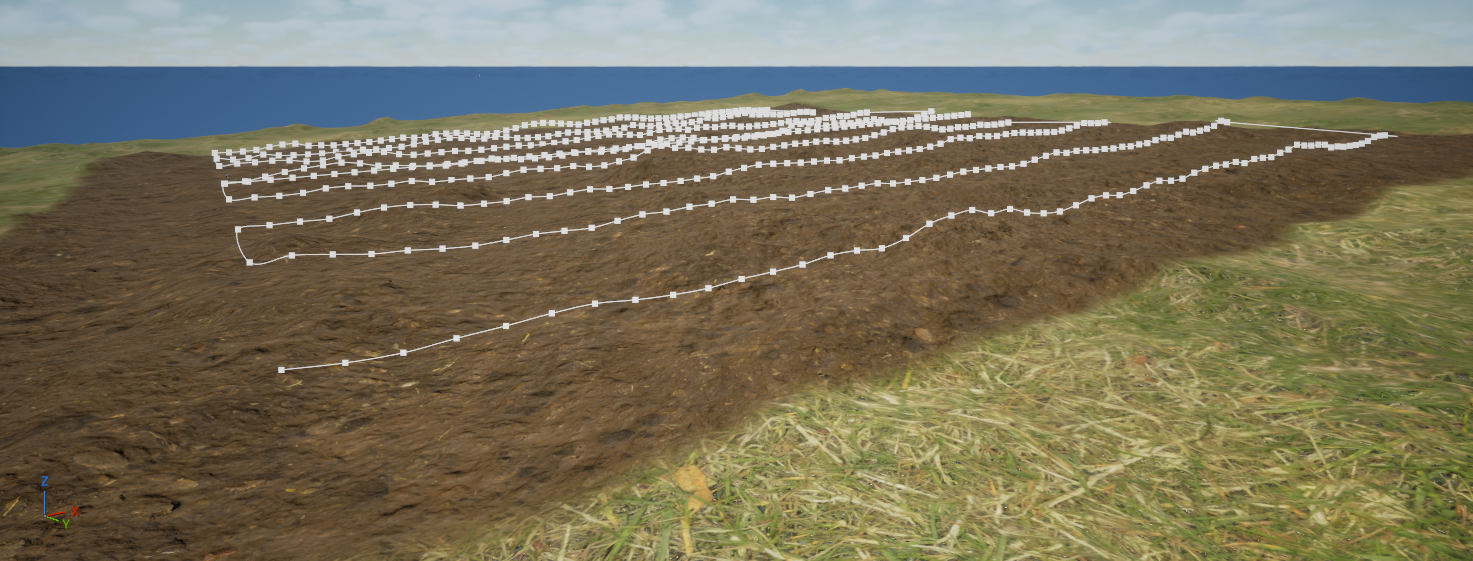
\includegraphics[width=\linewidth]{images/spline_uneven.png}
        \caption{Spline points adapting to the morphology of the ground, making the camera also follow this trail, as if it is mounted onto a vehicle.}
        \label{splunev}
    \end{subfigure}
    
    \caption{Spline points automatically generated based on the dimensions of the field.}
    \label{spline}
\end{figure}


\subsection{Unreal Engine's Sequencer}

Sequencer is a cinematic workflow that allows manipulation of actors. Including a Cine Camera Actor also enables capturing frames of the scene, as the actions described in the Sequencer's actor parameter handling tab are performed. After the parameters are set, rendering can be performed, extracting multiple sequential frames, either in the form of separate images or video.

By adding the aforementioned spline actor to the Sequencer, any actor, in our case the frame-capturing medium, can be attached onto it and follow the path that it defines. This was how SCC was able to traverse the whole field, storing the red and green band luminance of any defined point. It is important to mention that, as discussed in Subsection~\ref{findlum}, using Cine Camera Actor was not possible, despite the amount of tools supporting it within the Sequencer. Although the Cine Camera Actor is capable of rendering linear images, the color it renders is heavily processed, making it incompatible with the light meters' readings.

Sequencer programs the events occurring during the execution of a sequence primarily based on the frames that are programmed to be rendered by a Cine Camera Actor, even if one is not added to the sequence. Therefore, the movement of objects is simulated by defining where each moving object shall be whenever a frame is about to be captured, arranged sequencer events are triggered whenever a frame is about to be captured etc. This was particularly useful for setting up the sampling frequency of the data recording tools, ensuring that SCC captures and actor-position samples were acquired synchronously at a fixed frame-based frequency.

\subsection{Scene Capture Component}

Although Sequencer provides multiple tools dedicated to rendering images using a Cine Camera Actor in an automated fashion, there is a lack of components providing a similar functionality for Scene Capture Components. However, since Sequencer was identified as the most convenient way for simulating the movement of objects, it was necessary to build the data collection around it, even while using SCC as the image rendering medium.

I overcame this problem with the discovery of Frame Capture Manager, a C++ class actor that, as mentioned, makes the ability of SCC to save images to disk visible to other actors. Specifically in this case, the instance of Frame Capture Manager that I added to the digital twin is visible to the Sequencer and, by creating a custom event that triggers at the same rate a Cine Camera would render frames, CaptureNonBlocking is called, collecting automatically the data. The Blueprint of the frame-capturing pipeline is illustrated in Figure~\ref{bluep}.

\begin{figure} [htb]
    \centering
    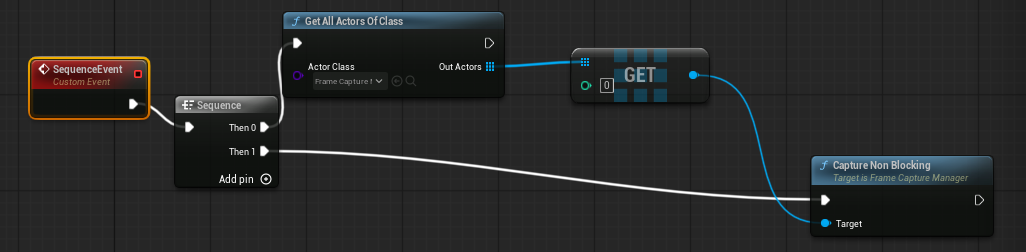
\includegraphics[width=1\linewidth]{images/image.png}
    \caption{Custom event triggering for every programmed frame of the Sequencer. It detects the Frame Capture Manager and calls the function responsible for rendering frames, CaptureNonBlocking. }
    \label{bluep}
\end{figure}

The distance covered by the SCC actor between two separate function calls is fixed. That means that the coordinates of SCC whenever it renders an image remain the same between separate sequences, both when the actor is moving from the start of the spline to its end and the opposite. Consequently, I considered it interesting to also compare GRVI values, as they are measured in these two cases. A simplistic way of achieving this was by setting up the camera's pitch in such a way that the center of its lens is targeted in the middle of the distance between two sequential camera points, essentially calculating the angles of a right triangle whose vertical side is the distance of the camera from the ground and its horizontal side is the distance between the projection of the camera to the ground and the middle of the distance between two consecutive frame-capture positions. It is important to note here that the vertical distance between the camera and the ground was selected instead of the vertical distance between the camera and the field's canopy because the inclusion of the plants' stems, which are more occluded than the canopy, and the field's soil, which, due to its color, adds red-band luminance to the calculated average GRVI of the point of interest, make the model more robust. The pitch of the camera is the angle between the vertical side of the triangle and the hypotenuse, multiplied by negative one ($-1$) (Figure~\ref{camangle}).

\begin{figure} [htb]
    \centering
    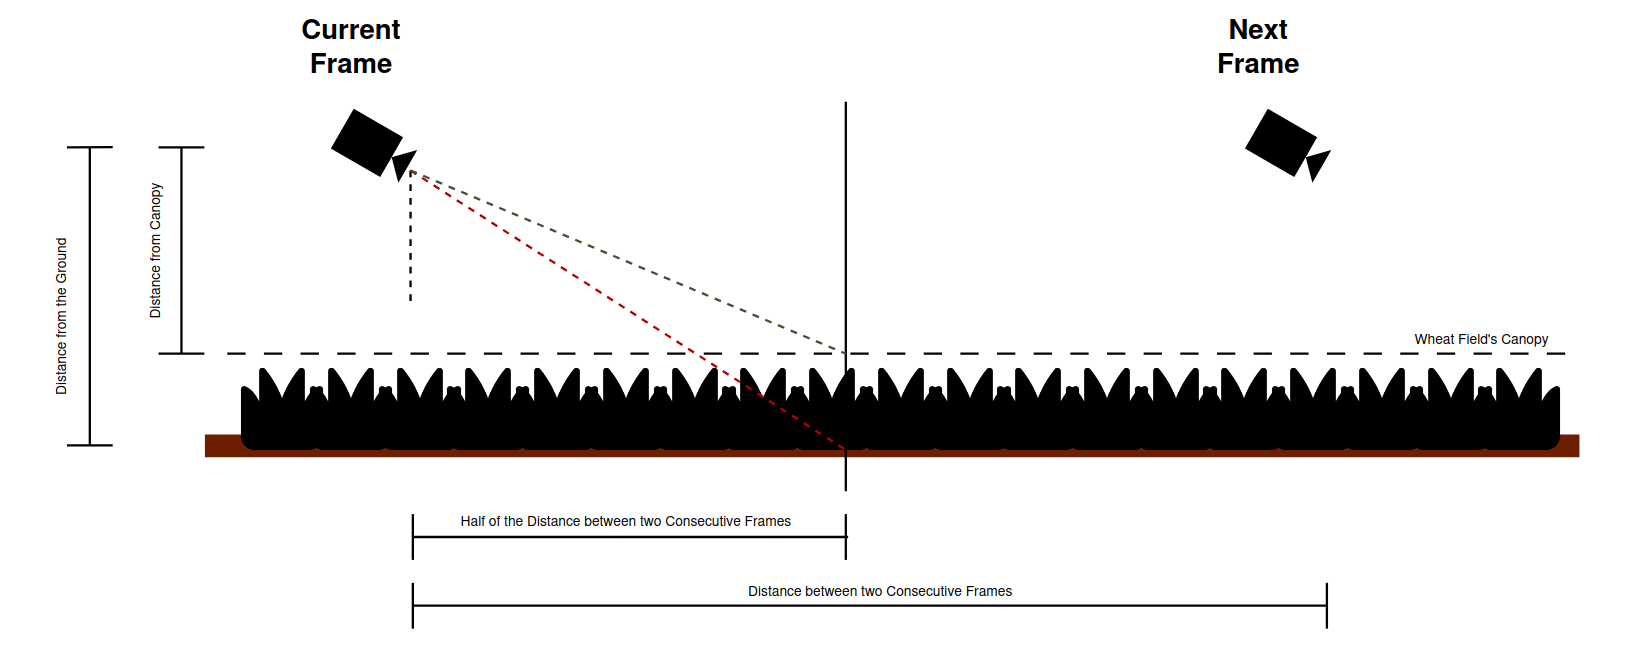
\includegraphics[width=1\linewidth]{images/cameraangle_diag.png}
    \caption{Diagram illustrating how the camera's pitch was calculated. The viewing angle calculated using the distance from the ground is represented by the red dashed line, while the green dashed line represents the angle calculated from the canopy. The first distance captures more comprehensive field data, making the model more robust, and thus was selected.}
    \label{camangle}
\end{figure}

The distance of the SCC from the ground is set to two meters, and the distance between two consecutive frames is approximately 1.4 meters, therefore the sensor's pitch was set to $-20^\circ$. 

\subsection {Light Meters' Position and Readings}

Originally, there were no obstacles between the simulated sun and the field, making the illuminance even across the scene. That meant that a single stationary light meter was sufficient for providing enough information for the whole scene. As an extension of the dataset was developed, including trees that cast shadows over the crop's canopy in several parts of the digital twin, illuminance can differ from point to point. This variance introduced the need to measure illuminance for each examined point of interest. 

To tackle this, I included additional light meters to the project, all attached to the same spline that SSC follows. In a real-world application, the light meters and the camera would be mounted on the same physical rig, making the measurement of the illuminance in the area-of-interest imprecise. Taking advantage of the simulation's lack of physical constraints, the light meters have a slight lead relative to the camera, aiming to measure illuminance directly towards the point where SCC points at. As discussed in (!!!! change this, its moved to the ML parts) \hyperref[feature-engineering]{the Feature Engineering Section}, this simplifying assumption provided the trained models an overly precise context of the illuminance in the studied area, lowering the significance of the relative position of the sun and the camera. (!!!!!!!!!!! this might not be the case!!!!!!!!!) This factor could make the models less transferable to real-world applications. I perform a comparative analysis between the models trained to the data captured with a single light meter placed close to the camera and several light meters placed close to the area-of-interest in the (!!!!!!!!! add hyper-ref here to the chapter-section !!!!!).

Regarding their exact positioning, the light meters were placed approximately in such a distance from the sensor, that their reading corresponds to the center of SCC's field of view, which practically is the middle of the distance between two frames. They are horizontally spread, accounting for the differences in measured illuminance between different parts of the captured scene, considering that it is not guaranteed that either all of the points of interest or none of them will be affected by the shadow of a tree. To avoid repeating the same process with a single light meter attached close to the camera, I took the readings of the central light meter and shifted them backwards, matching each frame with the readings corresponding to the previous frame. Although simplistic, this successfully simulates two important edge cases observed when illuminance is not measured directly on the sensor's field of view: capturing a frame of a shaded surface, while the rig is still exposed to the sun, and the opposite, capturing a frame of an illuminated surface, while the rig is still under the shadow of an obstacle.

In order to store the light meters' readings, I added another Sequencer event. Specifically, each time a frame would be rendered, the measurements, coordinates (so that it can be matched with the appropriate frame) and name of each light meter is printed to UE's render logs. I also developed a PowerShell script, so that when UE's Movie Render Queue is done managing the sequence, the logs are parsed and the printed light meters' information is stored in separate files.

Another assumption that I made regarded the number of included light meters. Although the total number of points of interest per captured frame is twenty, all sharing the same vertical coordinate and being horizontally adjacent to one another, I decided to include only five light meters, each covering four consecutive points of interest. This was mainly implemented in order to avoid overloading the computer hardware resources during Movie Render Queue's execution, considering that for each frame, the information for all added light meter should be read and stored.

\subsection{Solar Zenith Angle and Camera Rotation}

There was one remaining factor for covering the minimum data necessary for providing an ML model a sufficient context of how to interpret the measured GRVI value for a part of the scene and how to approximate its ground truth value through it: the position of the sun relative to the camera's viewing geometry for each frame. Because the solar zenith angle remains constant for each distinct illumination scenario, I logged this metric once per scenario, later to be parsed by a preprocessing script. Camera rotation and coordinates, on the other hand, change from image to image, necessitating the constant recording of this information. By retaining the camera's absolute spatial coordinates when a frame is captured, it is simple to match this frame with the inherent GRVI value of the plants depicted in the frame, assisting with the construction of the noise-free dataset. Simultaneously, tracking the sensor's roll, pitch and yaw provides context about the sun's relative directional orientation at the moment of capture.

In order to achieve that, a Sequencer event quite similar to the one responsible for tracking the light meters' information was developed. This time, during each event trigger, SCC's roll, pitch, yaw and absolute coordinates are printed to the log, which is later parsed, saving the data for the construction of the datasets.

With the completion of this step, the data collection pipeline was finalized. A diagram of this process is illustrated in Figure~\ref{dc-pipe}.


\section{Data Assessment}

\label{datasssessment}

After the render sequences were complete, more than thirty thousand frames were captured. The next step was to evaluate whether they provide meaningful information about the studied phenomena. The primary criteria for the assessment of data were:

\begin{itemize}
    \item Whether SZA affected the perceived GRVI values of the vegetation captured in the frames (Subsection~\ref{sza-aff-grvi}).
    \item How does perceived GRVI behave under overcast lighting and are there differences between the inherent GRVI of distinct materials and their perceived counterparts (Subsection~\ref{diffuse-aff-grvi}).
    \item How do shadows affect GRVI (Subsection~\ref{shadows-aff-grvi}).
\end{itemize}

The answers to these questions served as the primary factors for determining whether the collected data were suitable for subsequent structuring and use in model training.

\begin{figure}[H]
    \centering
    
    \begin{minipage}{1\textwidth}

        \begin{subfigure}{\linewidth}
            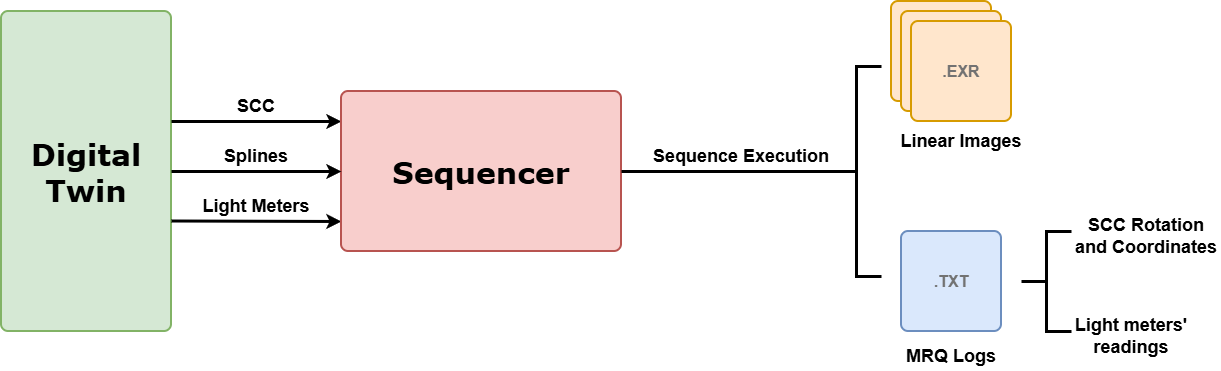
\includegraphics[width=\linewidth]{images/cd-pipe.png}
            \caption{The complete data collection pipeline.}
        \end{subfigure}
        
        \vspace{1em}
        
        \begin{subfigure}{\linewidth}
            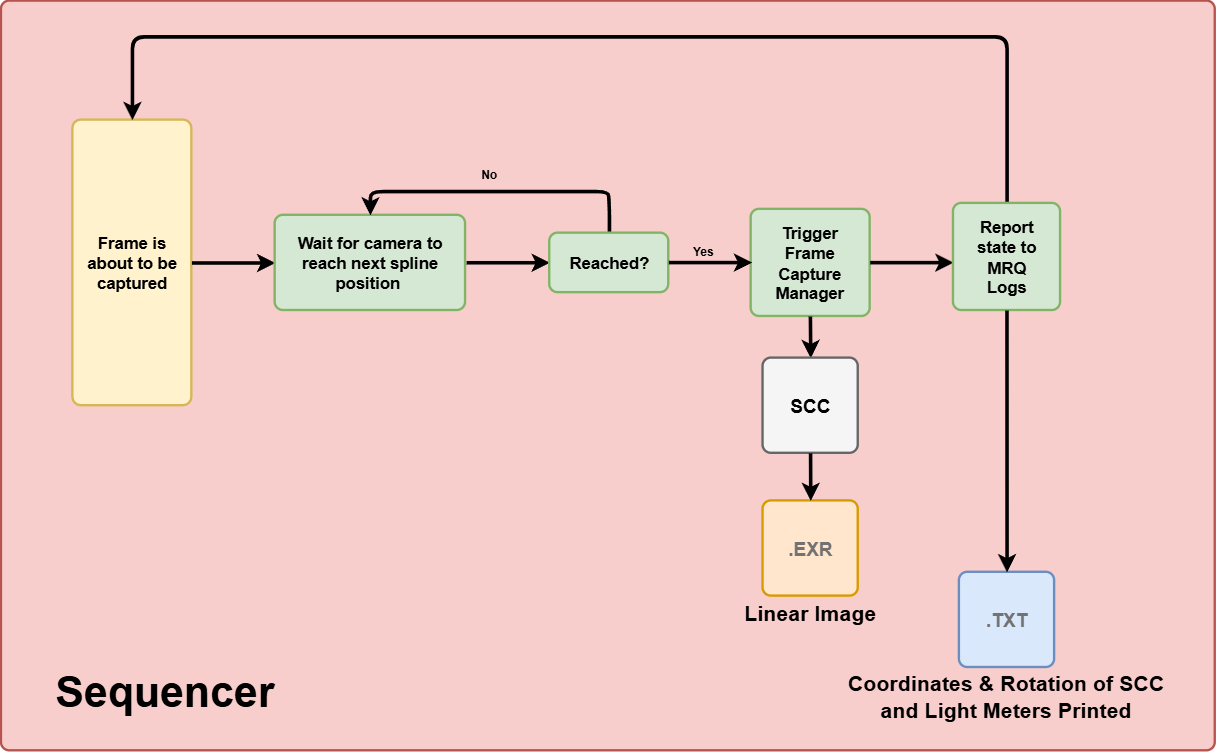
\includegraphics[width=\linewidth]{images/sequencer.png}
            \caption{The steps the sequencer follows for every step of the data collection.}
        \end{subfigure}
        
        \caption{The materials used for the digital twin's terrain, both isolated and combined.}
        \label{dc-pipe}
        
    \end{minipage}
    
\end{figure}

\begin{figure}
    \centering
    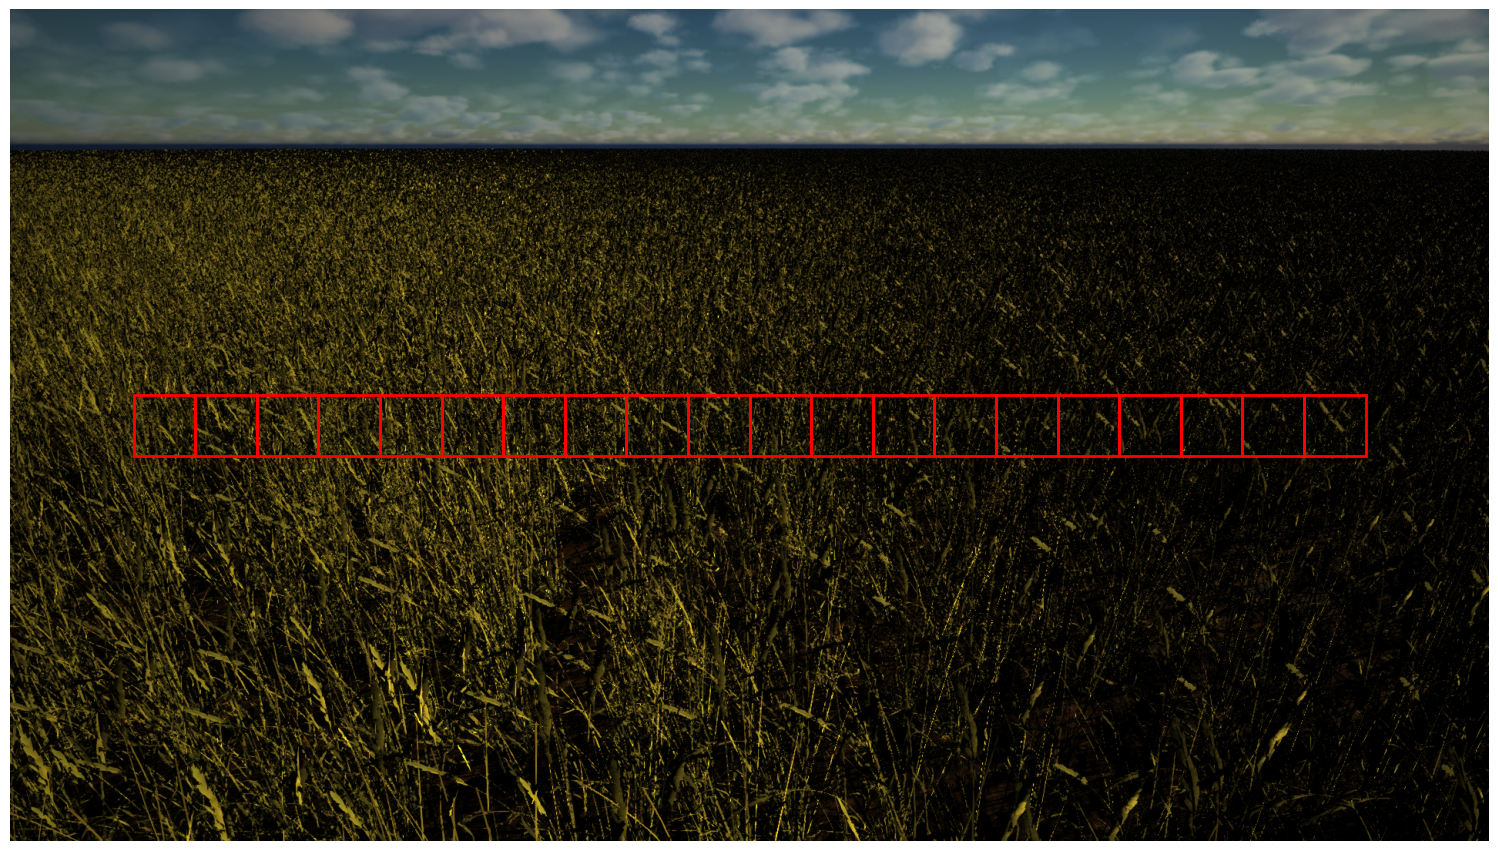
\includegraphics[width=1\linewidth]{images/6_img_lowGRVI.png}
    \caption{areas-of-interest in an image.}
    \label{aoi}
\end{figure}


In addition to the final rendering sequences, I performed several dummy sequences as well, aiming to test the material's properties, isolated from the influence of other materials. Dummy renders differed from the ones  performed for the final data collection by the fact that the SCC was attached to a straight line segment of the developed spline, rather than the full polyline. This was decided in order to examine one case at the time, rather than constantly changing the sun-sensor-canopy geometry. The spline segment was placed in the middle of the digital twin, extending from the lower horizontal bound of the simulated field to the upper one, ensuring that the effects of the SZA variation are not biased towards one side. For all the tests conducted, the areas-of-interest for which the GRVI values were calculated were twenty adjacent square regions arranged horizontally across the image, with a common vertical position corresponding to the vertical center of the frame (Figure~\ref{aoi}).

Another important distinction of the dummy renders is the higher planting density in comparison to the final render sequences. The reasoning behind this was to, at a certain degree, isolate the calculations from the influence of background soil, aiming to observe how each material appears in the scene. That said, parts where soil is visible were kept in an attempt to see how much background soil influences the calculations. Another major reason responsible for the differences in planting density was the difference in the hardware resources needed between dummy and final render sequences. Greater density results in larger overhead. However, dummy renders require significantly less resources due to the presence of fewer actors in the simulation (a grid of crops with different materials applied versus one large crop-block with one material applied) and fewer frames programmed to be captured.

%i can add images of the field during various szas in the addendix

\subsection{SZA Effects on GRVI Values}
\label{sza-aff-grvi}


The behavior of the perceived GRVI values of a field canopy as the SZA changes was one of the primary inspirations for this study. As discussed in Section~\ref{brdf}, a field's canopy





\noindent behaves as an anisotropic reflector. Consequently, depending on the directionality of the incident radiation flux, different amounts of luminance are reflected towards different directions, while the amount of illuminance reaching the surface remains constant. Since the reflectance calculated using the formula for Lambertian surfaces (Equation~\ref{lambertian}) does not account for the directionality of light, as that is a factor that does not affect surfaces that reflect equal amounts of light towards all directions, variations in the SZA cause variations in the calculated reflectance values and, eventually, the calculated GRVI. It was therefore crucial for this study that these variations appear within the digital environment and, most importantly, in the dataset. 

The first test I performed did not include data stored as training examples but rather frames that were captured illustrating the digital twin with only one plant material applied, for multiple materials. The data were captured while SZA was set to $104^\circ$, $-104^\circ$ and $20^\circ$ in sequence, and the green-band illuminance, as measured right above the canopy, was set to 1020. The camera was attached to the straight spline. The primary goal was to confirm that the directionality of light does actually affect perceived reflectance, but also to investigate how different materials are affected. After each data collection was complete, the average GRVI value for each area-of-interest was calculated.

The results were promising, with errors caused by the directionality of the sun being apparent for every material I tested. Interestingly enough, depending on the inherent GRVI values of the material, the effects of SZA variation were quite different. In Figure~\ref{highgrvigrid} for example, a relatively high GRVI material (the highest appearing in the GRVI map, being 0.38) was set to the digital twin's meshes. Setting the SZA to $-104^\circ$ resulted in the right half of the field appearing more occluded than the left (Figure~\ref{6highimg}). This effect was also represented in the average GRVI per area-of-interest graphs, with the occluded part having overall lower GRVI values than the rest (Figure~\ref{6highgraph}). Specifically, the graph exhibits a downward trend towards the edge of the occluded region, with the boundary-adjacent area-of-interest exhibiting the lowest GRVI value. Similar results were observed when setting the SZA to $104^\circ$. This time, the left part of the field was occluded, having overall lower GRVI values. 

\begin{figure}[htb]
    \centering

    \begin{subfigure}{0.3\textwidth}
        \centering
        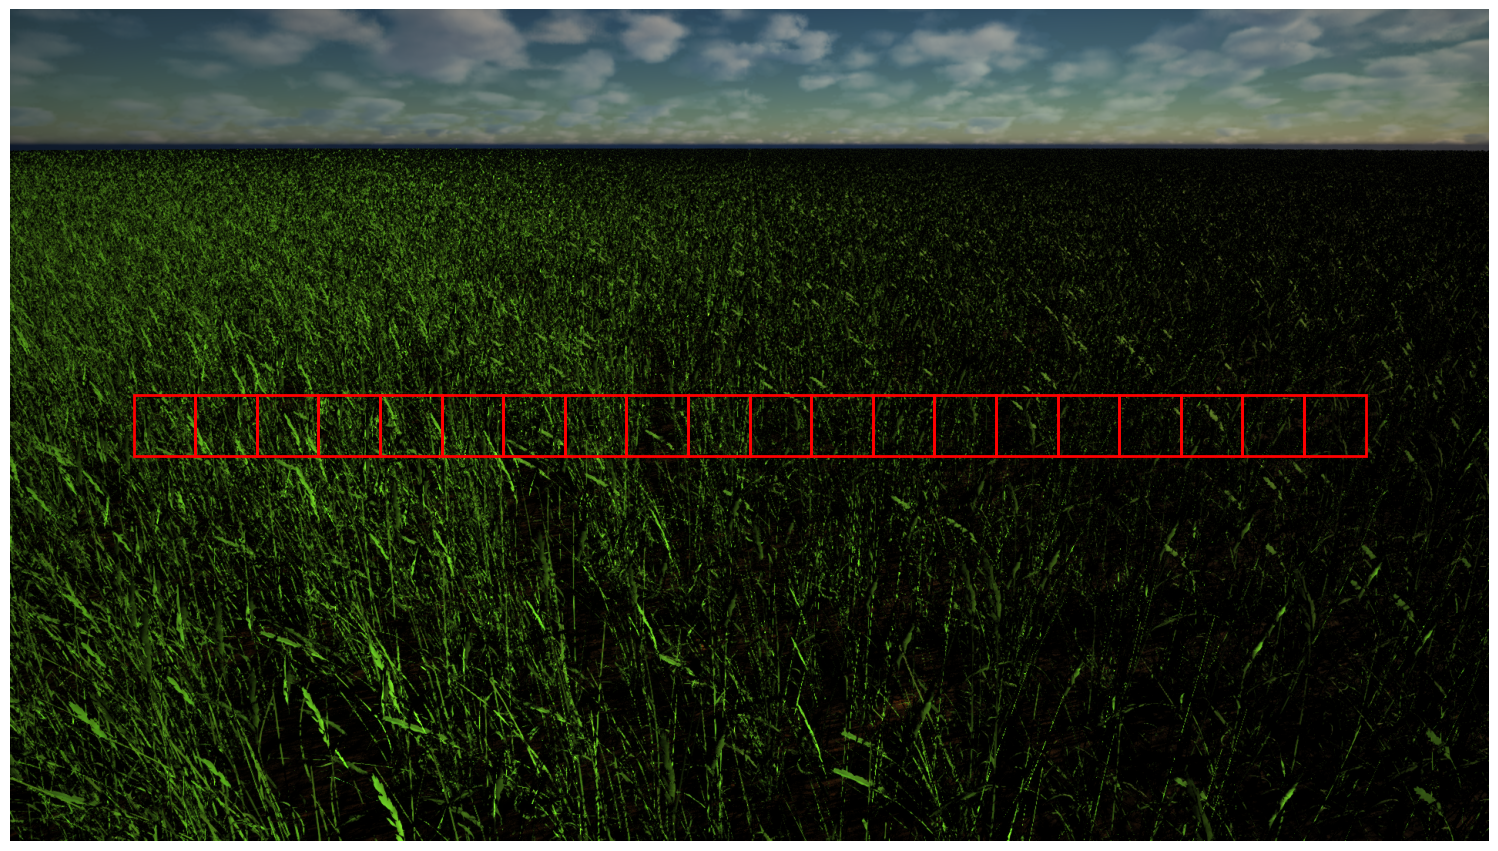
\includegraphics[width=\linewidth]{images/6_img_highGRVI.png}
        \caption{$-104^\circ$}
        \label{6highimg}
    \end{subfigure}
    \hfill
    \begin{subfigure}{0.3\textwidth}
        \centering
        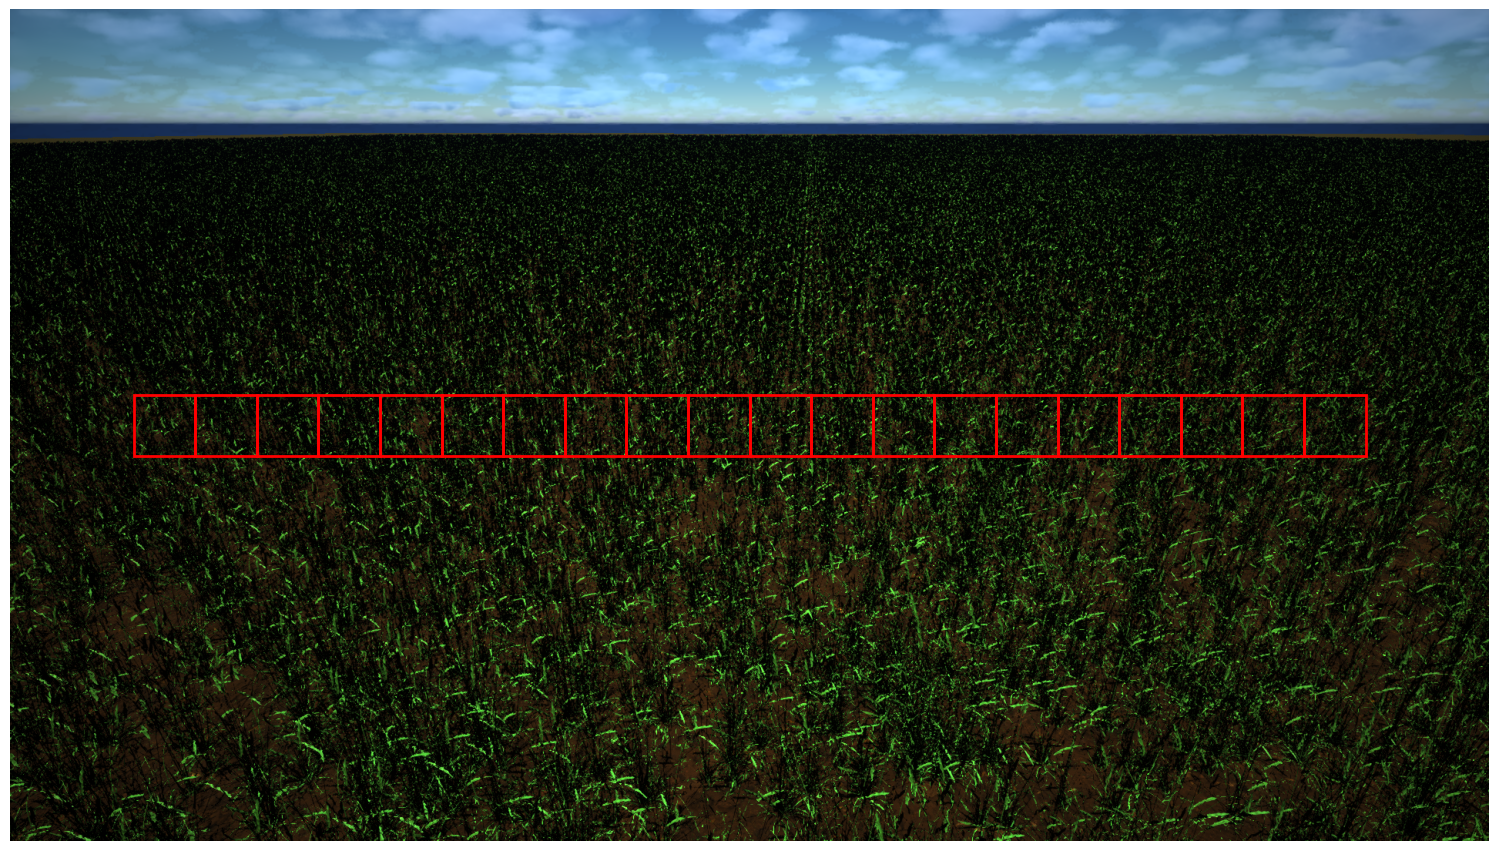
\includegraphics[width=\linewidth]{images/12_img_highGRVInc.png}
        \caption{$20^\circ$}
        \label{12highimg}
    \end{subfigure}
    \hfill
    \begin{subfigure}{0.3\textwidth}
        \centering
        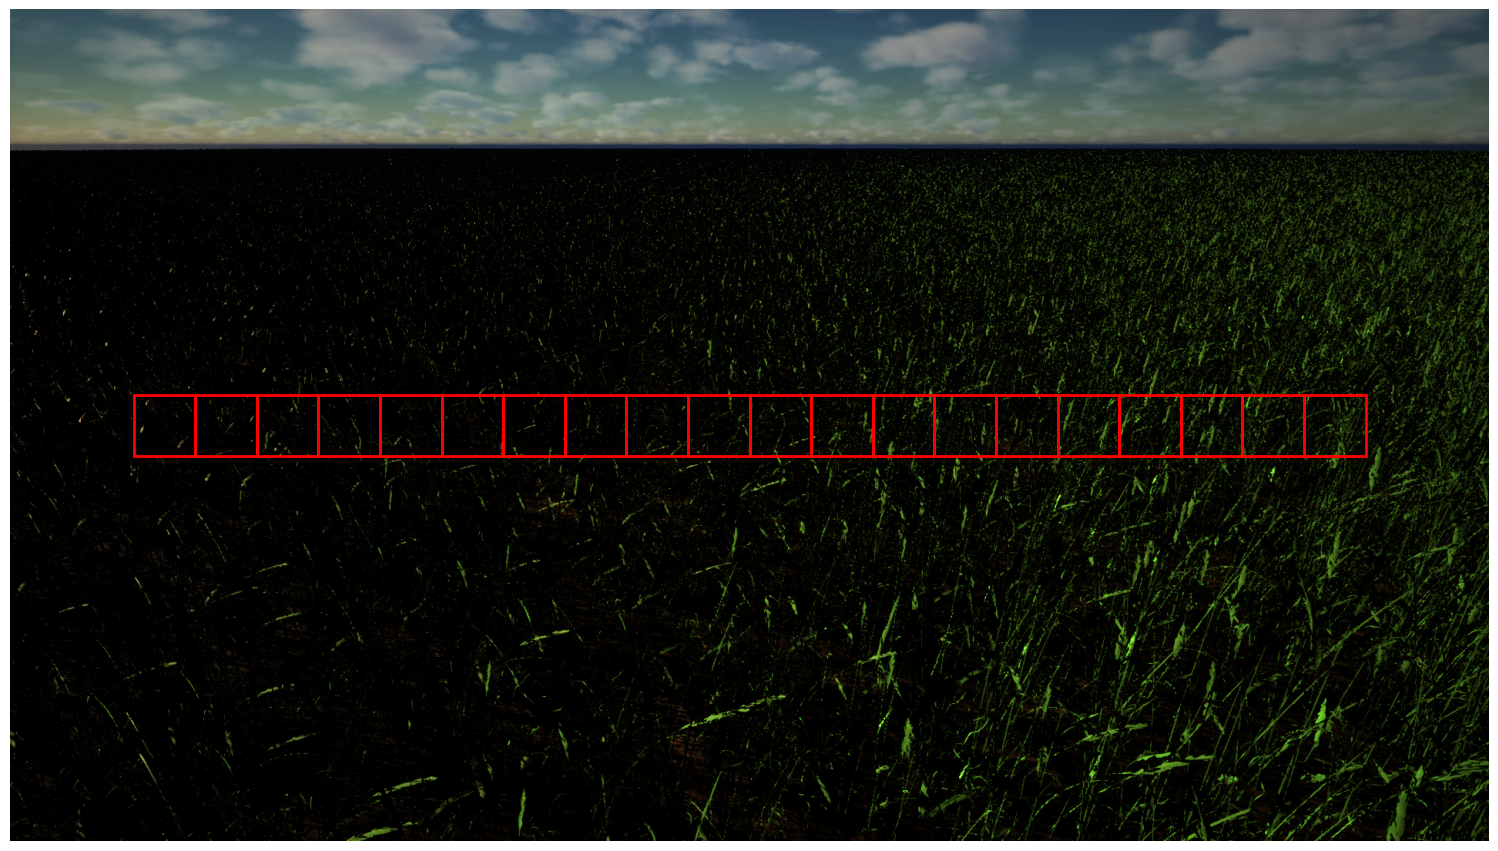
\includegraphics[width=\linewidth]{images/1715_img_highGRVI.png}
        \caption{$104^\circ$}
        \label{1715highimg}
    \end{subfigure}

    \vspace{0.5cm}

    \begin{subfigure}{0.3\textwidth}
        \centering
        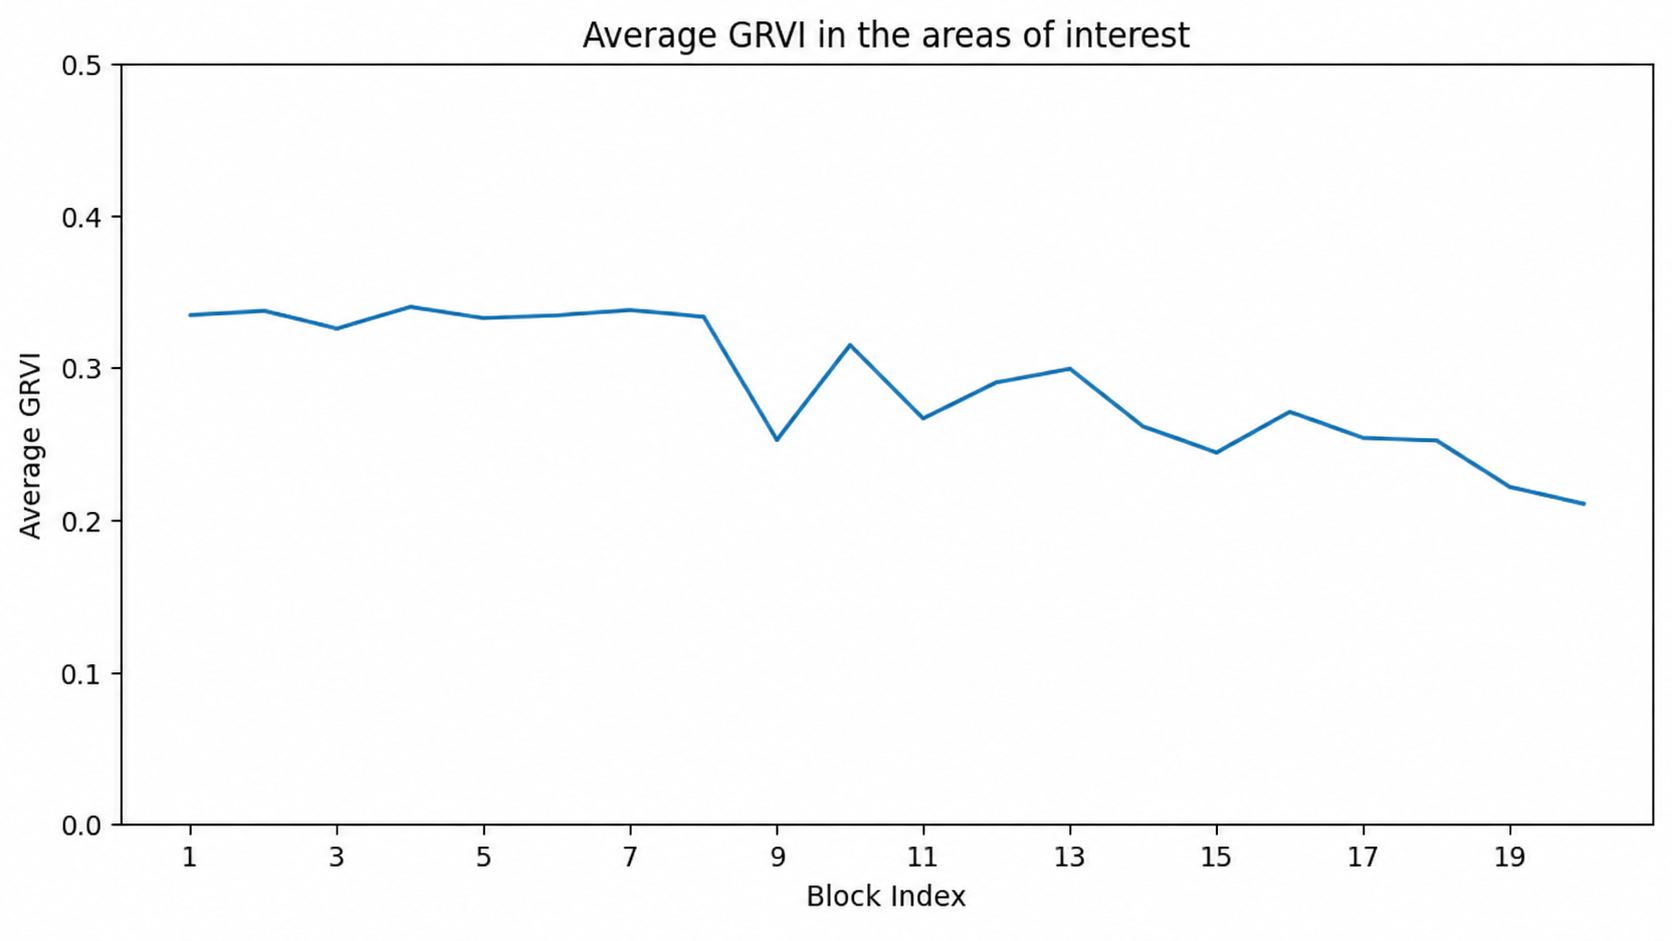
\includegraphics[width=\linewidth]{images/6_graph_highGRVI.png}
        \caption{$-104^\circ$}
        \label{6highgraph}
    \end{subfigure}
    \hfill
    \begin{subfigure}{0.3\textwidth}
        \centering
        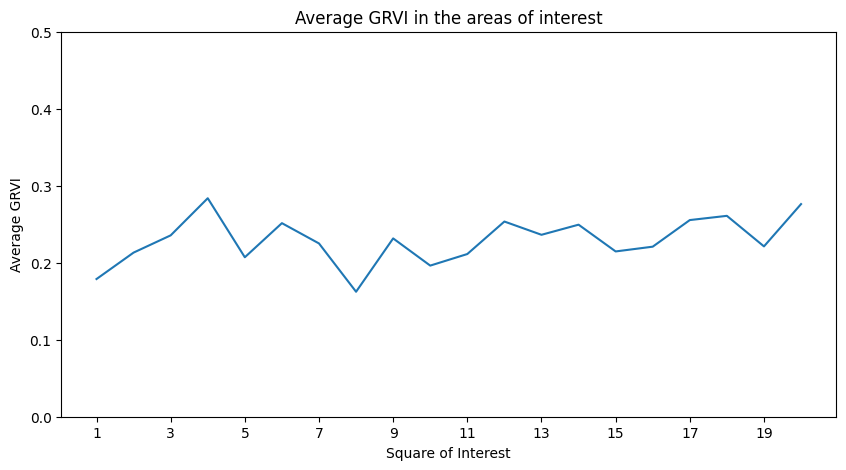
\includegraphics[width=\linewidth]{images/12_graph_highGRVInc.png}
        \caption{$20^\circ$}
        \label{12highgraph}
    \end{subfigure}
    \hfill
    \begin{subfigure}{0.3\textwidth}
        \centering
        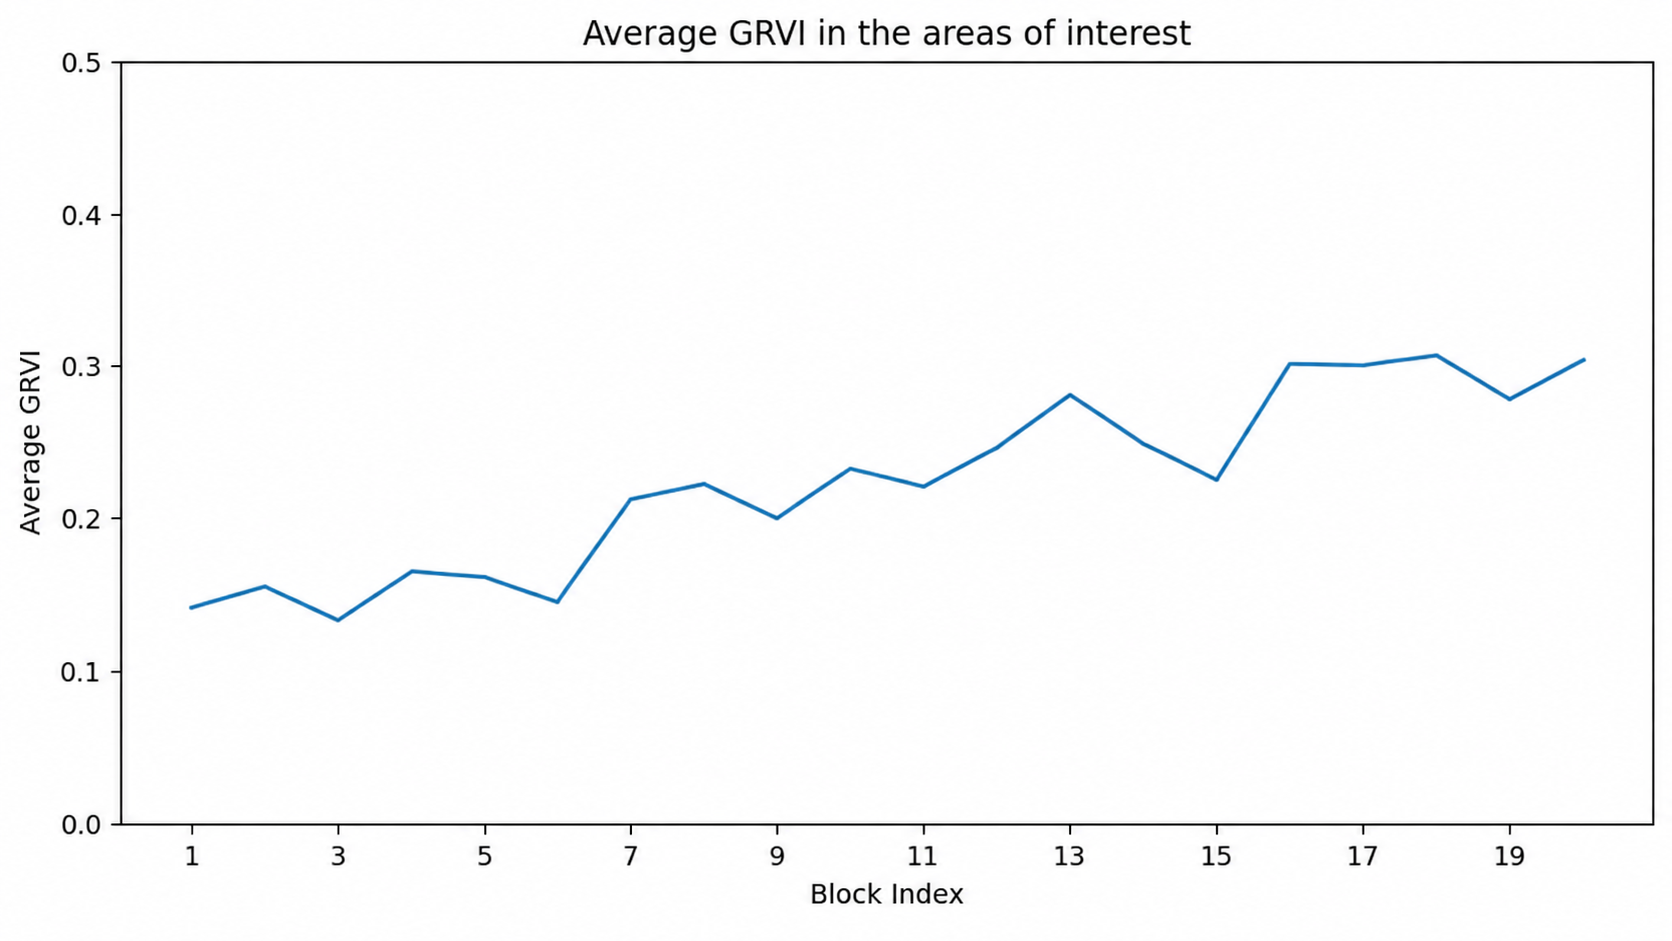
\includegraphics[width=\linewidth]{images/1715_graph_highGRVI.png}
        \caption{$104^\circ$}
        \label{1715highgraph}
    \end{subfigure}

    \caption{Images captured under various SZAs. The red squares indicate the bounds of the areas-of-interest. The corresponding graphs present the mean GRVI calculated for the same indexed areas-of-interest across all captured frames. The material used for the illustrated plants has an inherent GRVI of 0.38.}
    \label{highgrvigrid}
\end{figure}

The average values of the images captured with SZA set to $20^\circ$ manage to depict several of the rest of the factors that introduce noise to the measurements, including the uneven planting density of the crops, which results in more soil being visible and, consequently, dips in the average GRVI (for instance, in areas-of-interest with index 5 and 8 in Figure~\ref{12highimg}), and the dependency on the camera viewing geometry. Since the directional light is not angled, we see that there is no downward trend in the GRVI graph towards one of the sides of the image, the way it occurs for the other two cases ($-104^\circ$ and $104^\circ$).

The exact opposite results were observed while conducting the same experiments using low GRVI materials regarding the effects of SZA. As illustrated in Figure~\ref{lowgrvigrid}, this time GRVI values follow an upward trend within the occluded region, with a way smaller absolute difference between the GRVI values rightmost and leftmost. This time, the average GRVI values for SZA equal to $20^\circ$ were barely above the highest value recorded in the occluded part of the field (Figure~\ref{12lowgraph}.

\begin{figure}[htb]
    \centering

    \begin{subfigure}{0.3\textwidth}
        \centering
        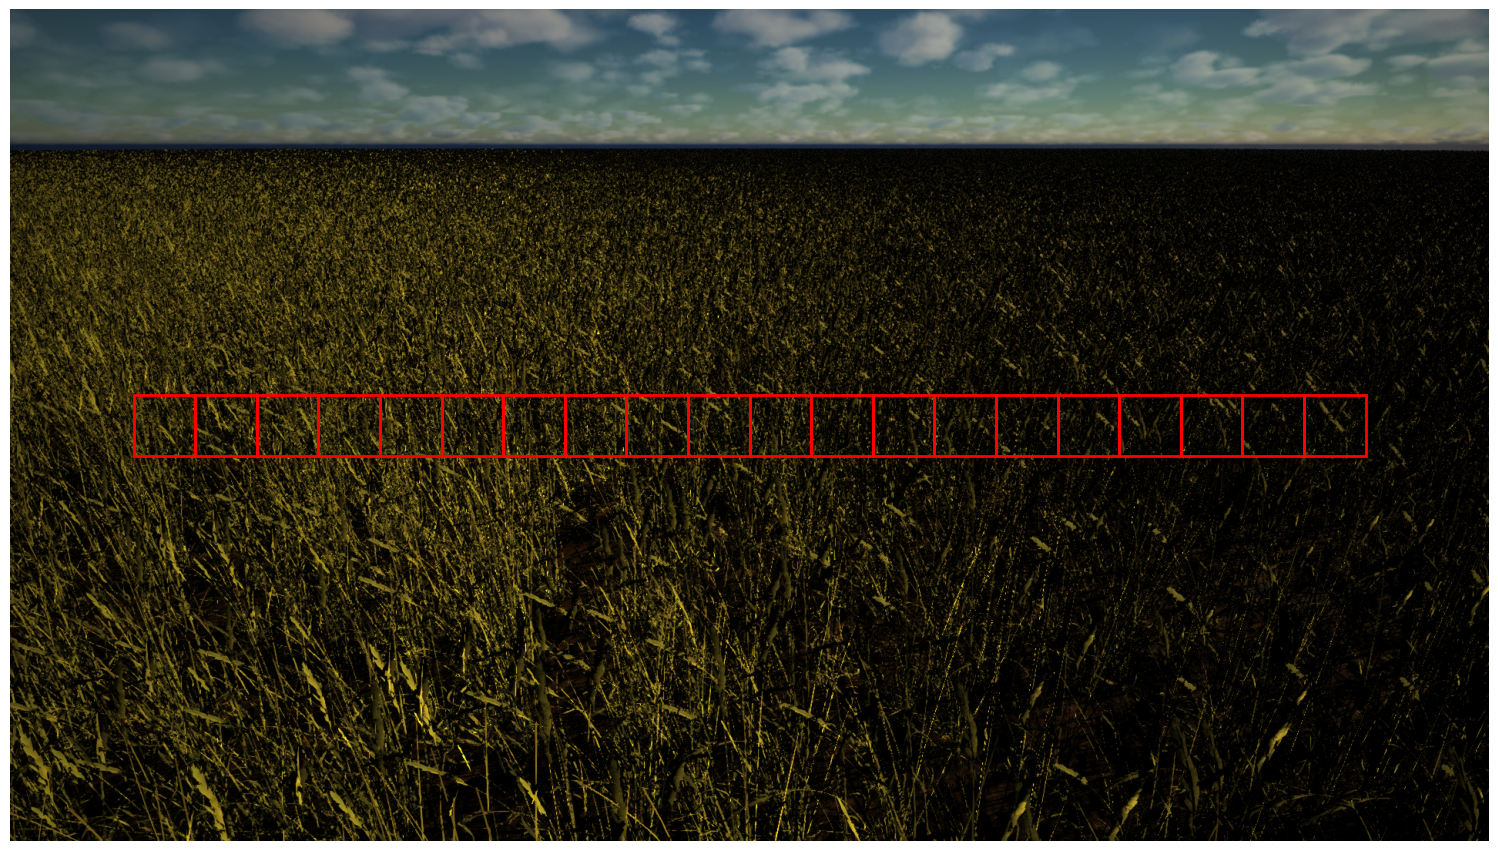
\includegraphics[width=\linewidth]{images/6_img_lowGRVI.png}
        \caption{$-104^\circ$}
        \label{6lowimg}
    \end{subfigure}
    \hfill
    \begin{subfigure}{0.3\textwidth}
        \centering
        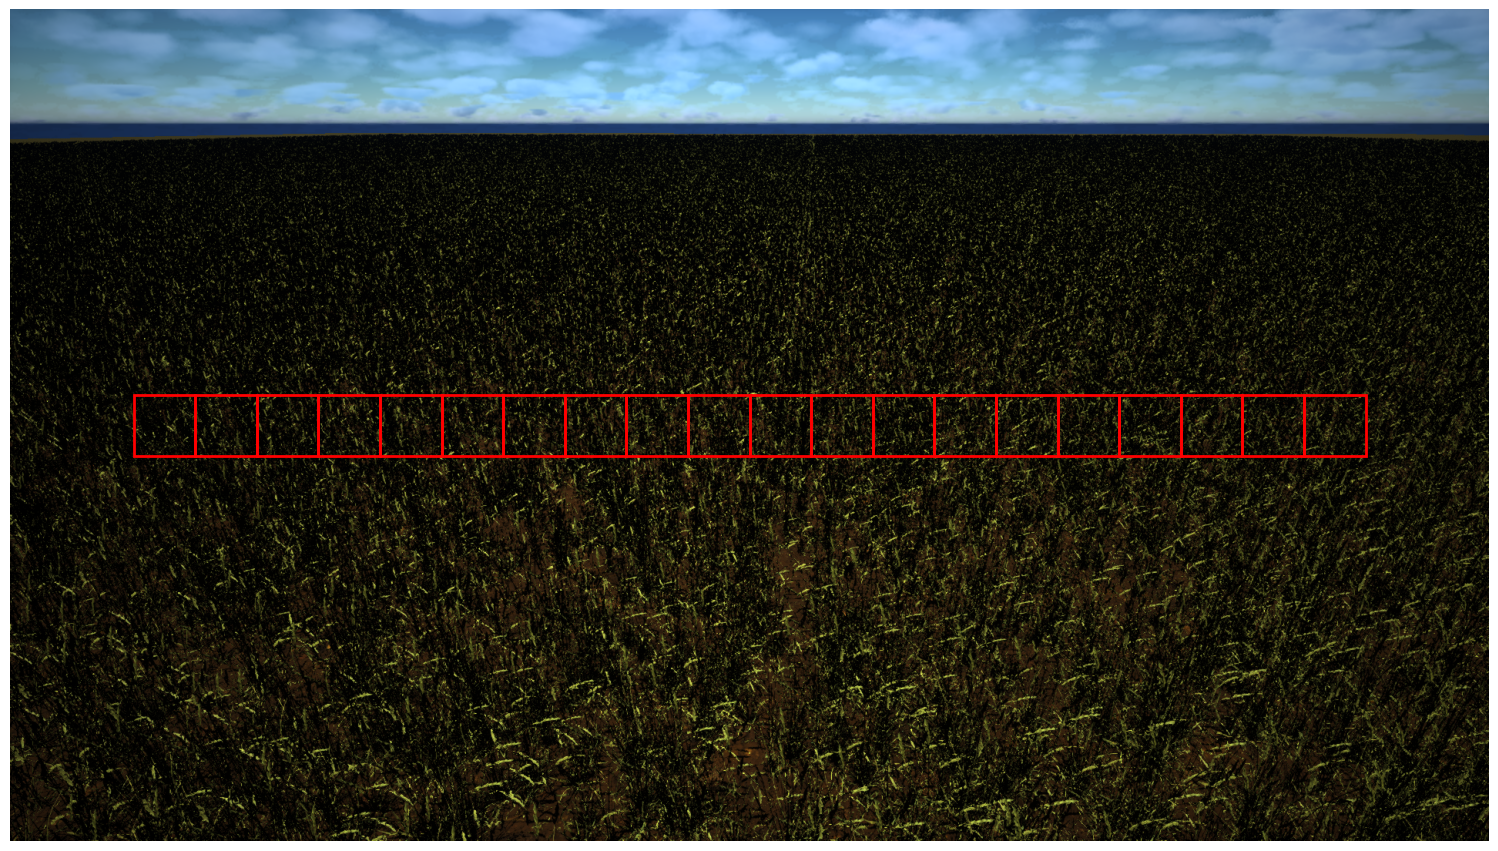
\includegraphics[width=\linewidth]{images/12_img_lowGRVInc.png}
        \caption{$20^\circ$}
        \label{12lowimg}
    \end{subfigure}
    \hfill
    \begin{subfigure}{0.3\textwidth}
        \centering
        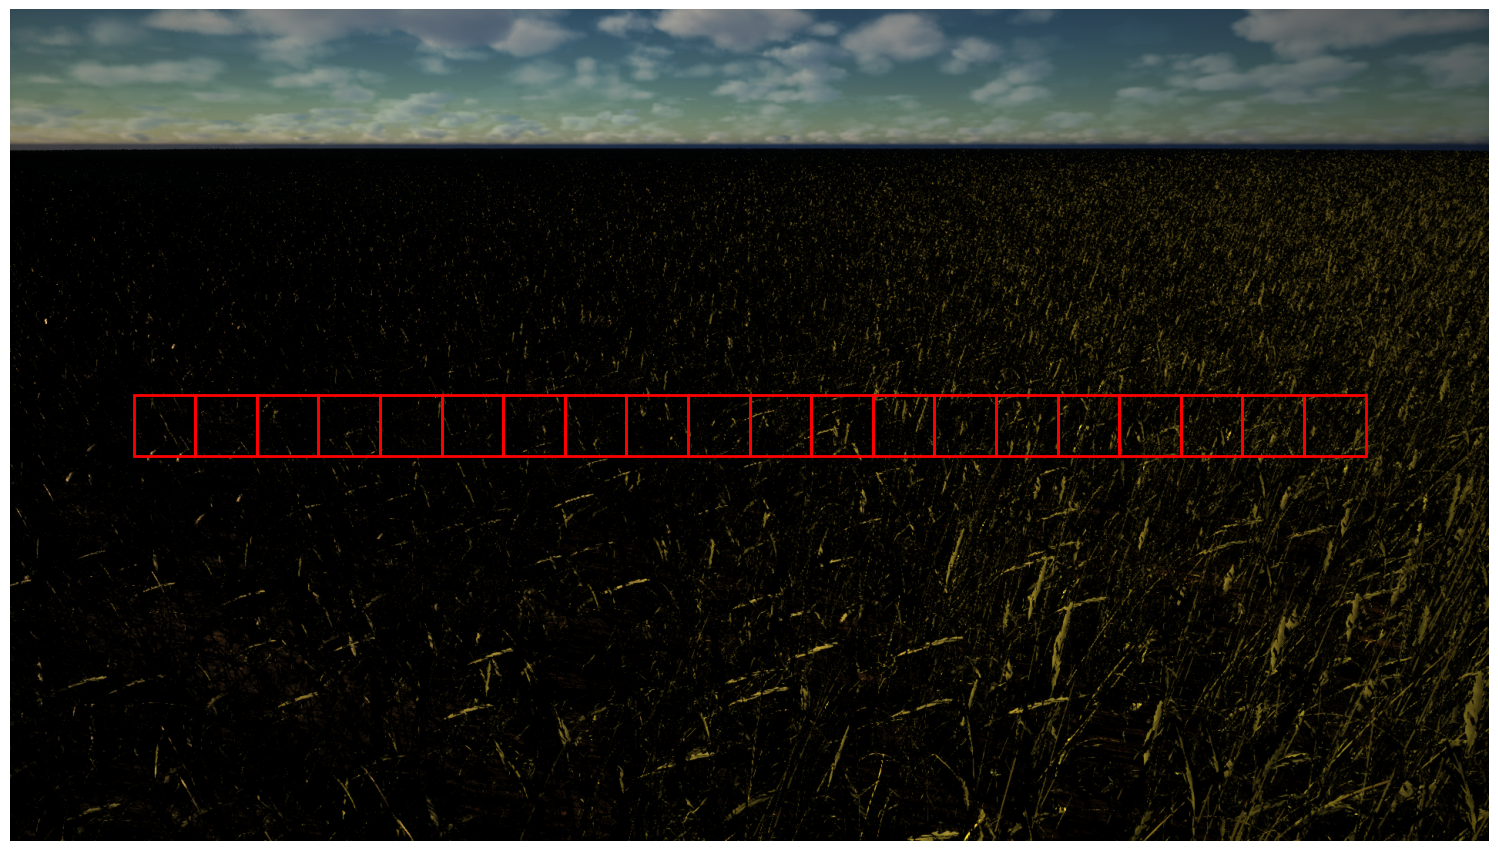
\includegraphics[width=\linewidth]{images/1715_img_lowGRVI.png}
        \caption{$104^\circ$}
        \label{1715lowimg}
    \end{subfigure}

    \vspace{0.5cm}

    \begin{subfigure}{0.3\textwidth}
        \centering
        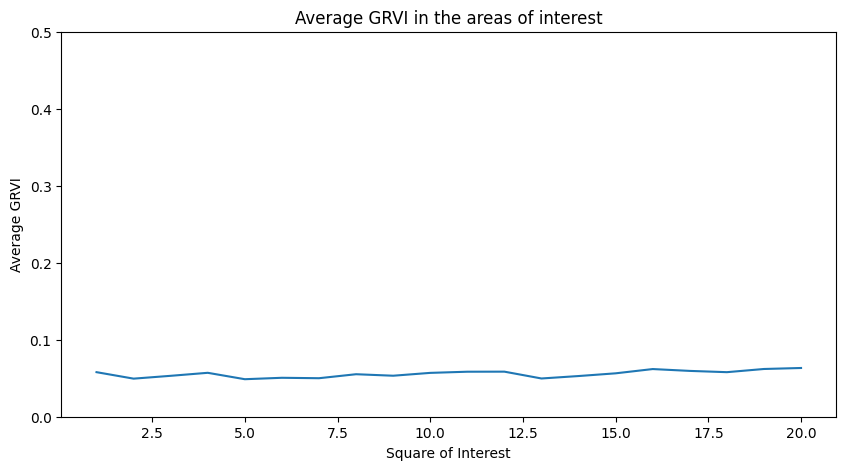
\includegraphics[width=\linewidth]{images/6_graph_lowGRVI.png}
        \caption{$-104^\circ$}
        \label{6lowgraph}
    \end{subfigure}
    \hfill
    \begin{subfigure}{0.3\textwidth}
        \centering
        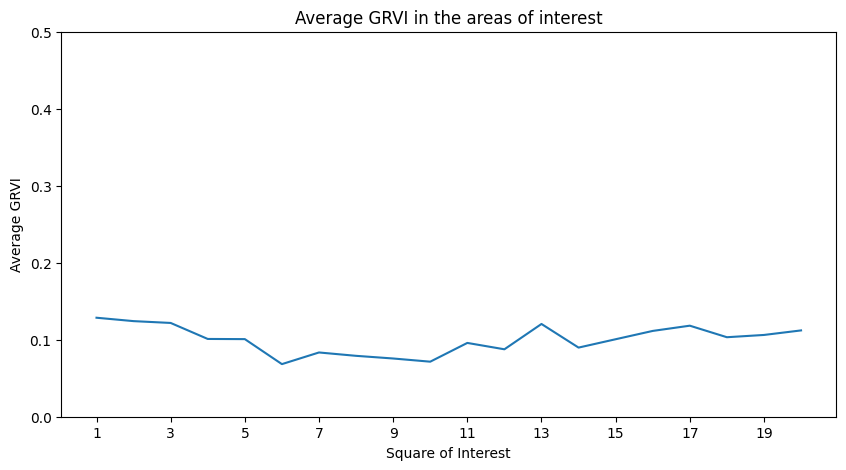
\includegraphics[width=\linewidth]{images/12_graph_lowGRVInc.png}
        \caption{$20^\circ$}
        \label{12lowgraph}
    \end{subfigure}
    \hfill
    \begin{subfigure}{0.3\textwidth}
        \centering
        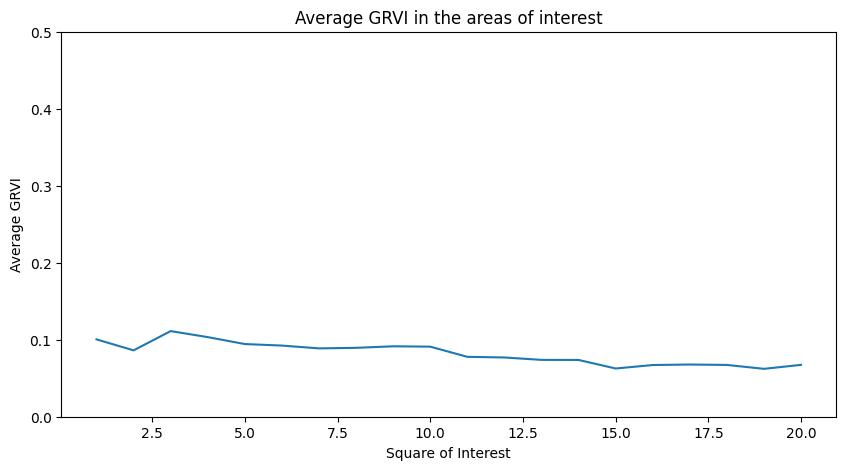
\includegraphics[width=\linewidth]{images/1715_graph_lowGRVI.png}
        \caption{$104^\circ$}
        \label{1715lowgraph}
    \end{subfigure}

    \caption{Images captured under various SZAs. The red squares indicate the bounds of the areas-of-interest. The corresponding graphs present the mean GRVI calculated for the same indexed areas-of-interest across all captured frames. The material used for the illustrated plants has an inherent GRVI of 0.08.}
    \label{lowgrvigrid}
\end{figure}

Overall, for all the materials I tested, there was a similar pattern observed: all bright-appearing parts of the images have roughly the same perceived GRVI value, with fluctuations caused by the viewing geometry, presence of soil and more, while measurements regarding the occluded part of the field follow an upward or downward trend towards the edge of the occluded region, depending on the material. To measure how much each material is affected  by the directionality of light, I used the percentile difference between the edge of the occluded part and the edge of the bright-appearing region:

\begin{equation}
    \%Diff = \frac{GRVI_O - GRVI_B}{GRVI_B}
    \label{nonsymDiff}
\end{equation}

With the SZA fixed at $104^\circ$ and green-band illuminance equal to 1020, the occluded part appears at the left side of the scene. The results of the measurements are illustrated in Figure~\ref{graphComp}.

\begin{figure} [htb]
    \centering
    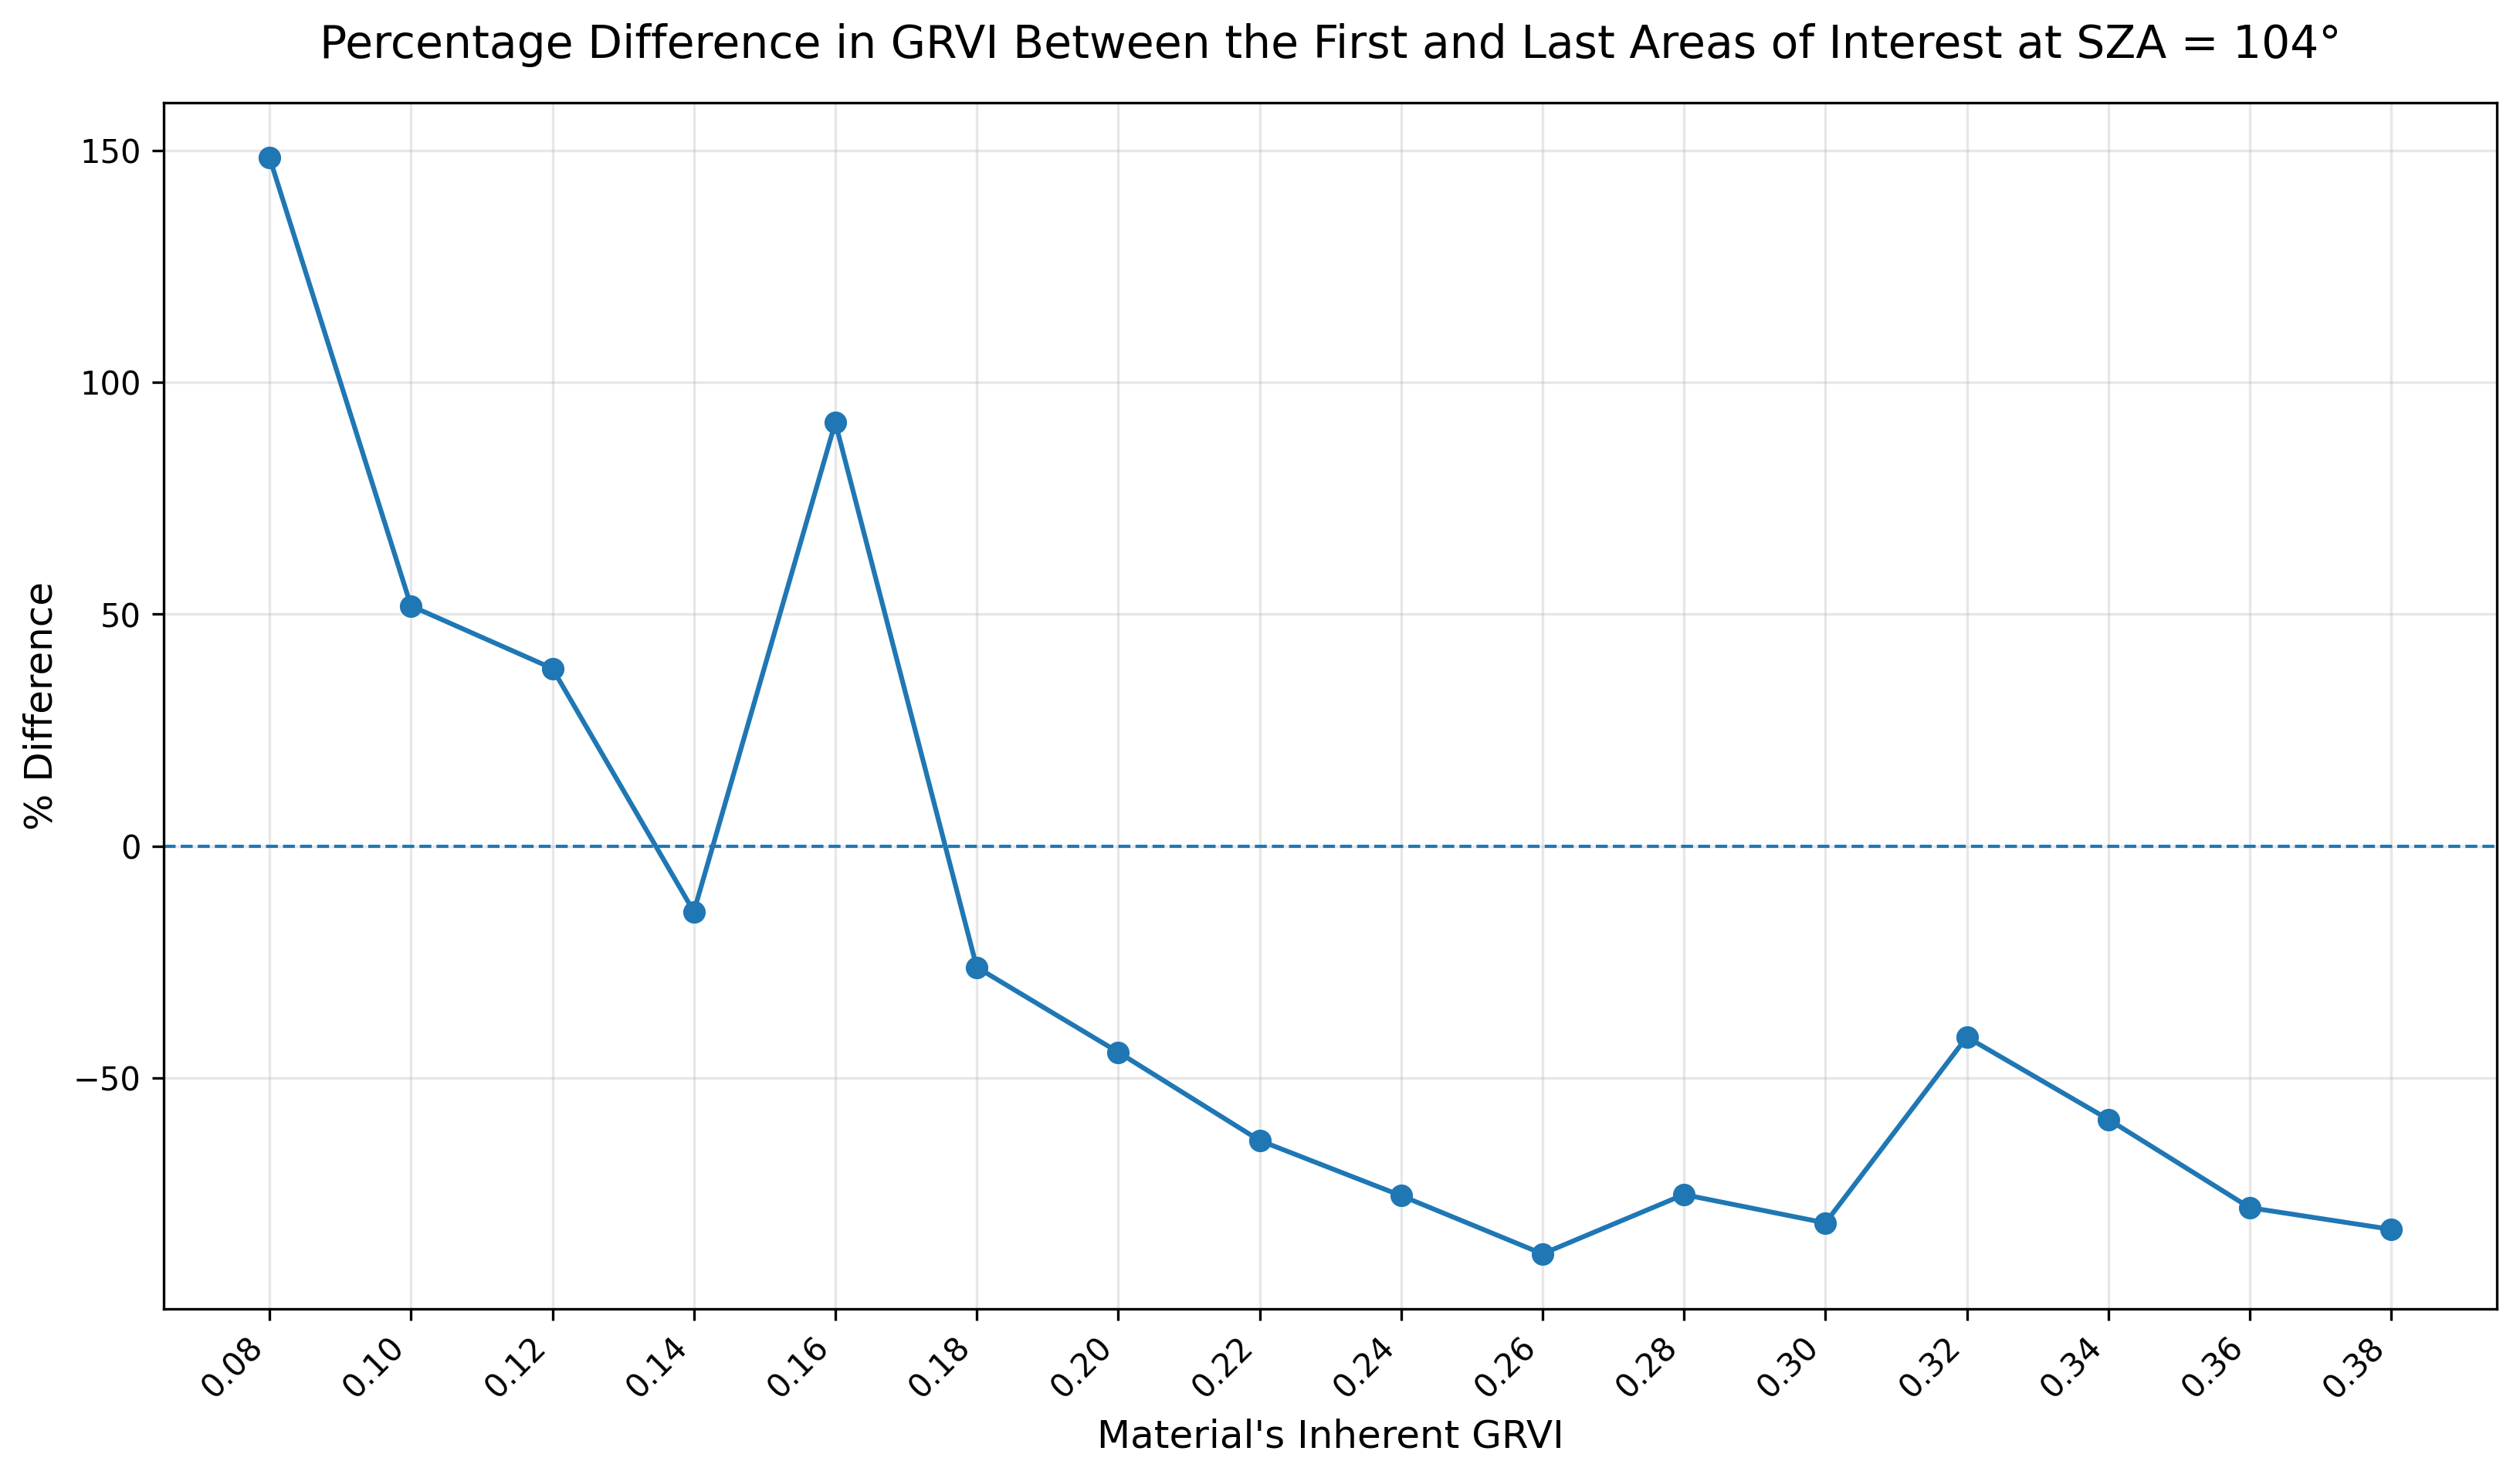
\includegraphics[width=1\linewidth]{images/grvi_percentage_difference_sza_104.png}
    \caption{Average Percentage difference between the rightmost and leftmost areas-of-interest of the captured images. Since the SZA was set to $104^\circ$, the first belongs to the bright-appearing region of the field, while the latter belongs to the occluded region of the frames.}
    \label{graphComp}
\end{figure}

The next test regarded the differences between two separate render sequences, one performed with SZA set to $-104^\circ$ and one with SZA set to $104^\circ$. Green-band illuminance remained at 1020. This time, the data collected from the final render sequences were used. The comparison was made between the areas-of-interest of the frames captured while SZA was set to $104^\circ$ and the areas-of-interest of their matching frames captured while SZA was set to $-104^\circ$. The difference between the measured values was expressed with the symmetric percent difference:

\begin{equation}
    \%Diff = \frac{|GRVI_{104} - GRVI_{-104}|}{\frac{|GRVI_{104}| + |GRVI_{-104}|}{2}}
    \label{symDiff}
\end{equation}


Whenever the difference between two areas-of-interest with the same index was calculated, the percentage was added to a common total for the specific index. By the end of the process, I divided the total for each index with the number of compared frames, resulting in the mean percentage difference for the specific index across the dataset. As discussed in Section~\ref{DC}, since during the final render sequences SCC follows a path defined by a spline that forms an orthogonal polyline traversing the whole field, the sun-canopy-sensor geometry changes over time. However, this should not affect the symmetric difference as long as the sensor's yaw remains either $0^\circ$ or $180^\circ$. I excluded cases where the sensor's yaw is neither $0^\circ$ nor $180^\circ$, since they are not part of this study.

\begin{figure} [htb]
    \centering
    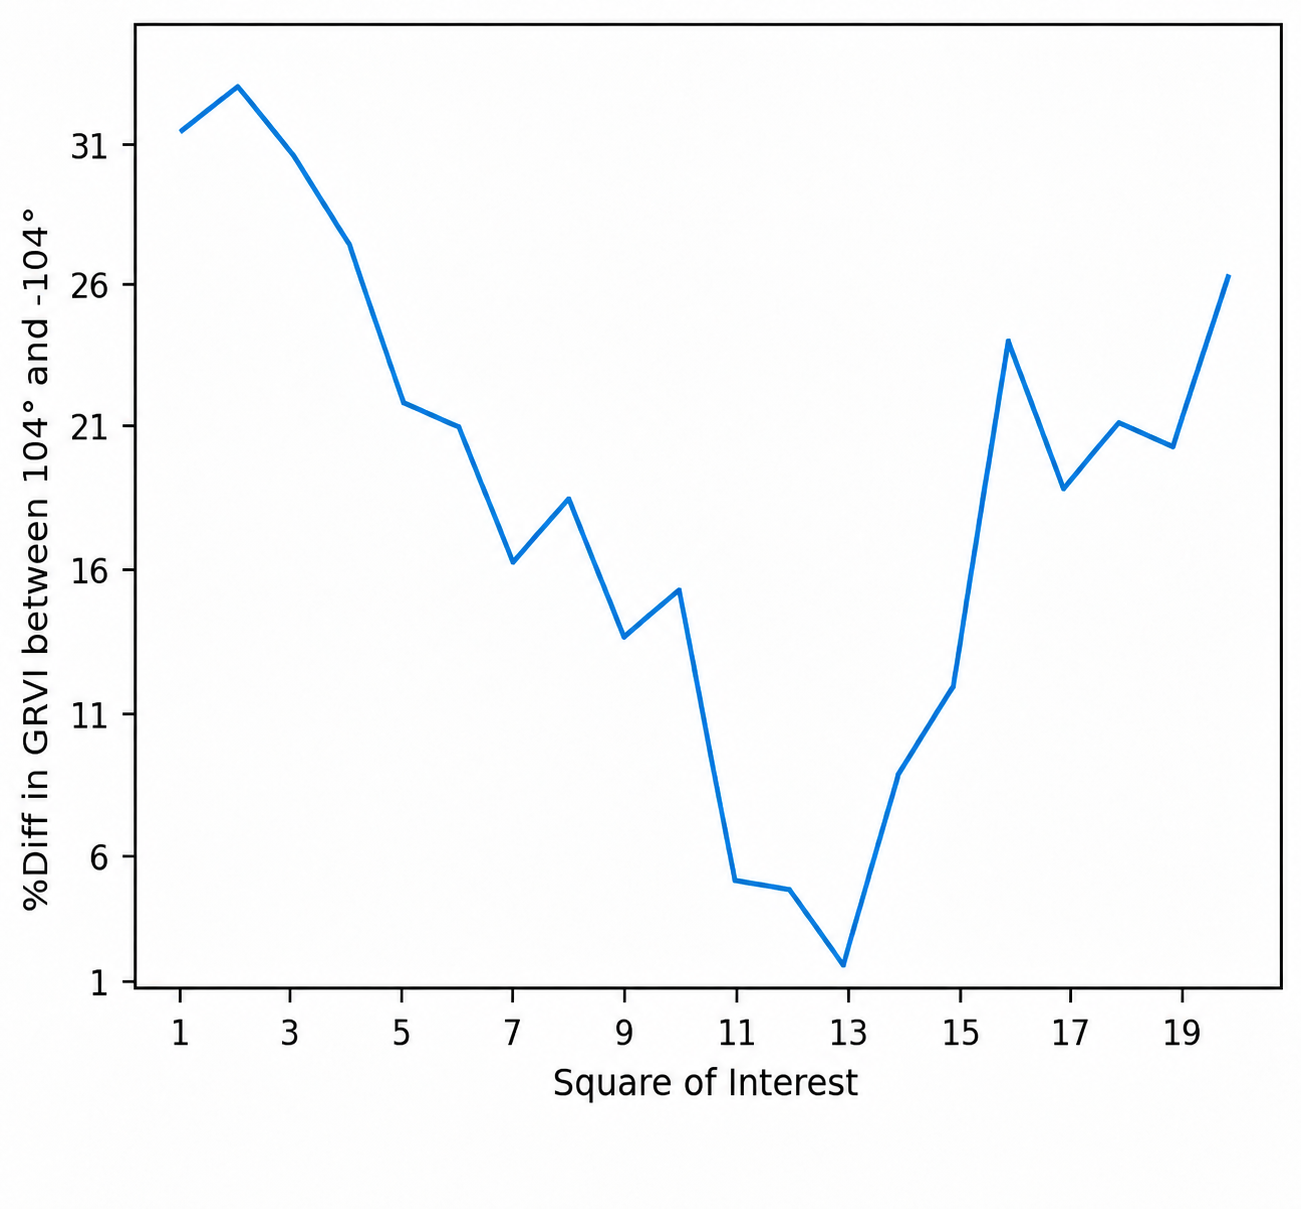
\includegraphics[width=1\linewidth]{images/104-104grviDiff.png}
    \caption{Average percentage difference between frames captured with SZA set to $104^\circ$ and $-104^\circ$. Comparisons are performed between corresponding areas-of-interest with the same frame index and the same within-frame index across different render sequences}
    \label{104-104}
\end{figure}

The results of this experiment are depicted in Figure~\ref{104-104}. As shown, areas closer to the bounds of the frame tend to differ more than areas closer to the middle. The reason behind that is that, closer to the middle, there is an overlapping region for both of the angles with equal magnitude and opposite signs, where the field appears almost equally bright. Consequently, percentage difference in this region is relatively low. On the other hand, regions closer to the bounds appear bright for one of the  cases and occluded for the other, with the difference becoming more evident as we approach the edge.

With these tests complete, it is apparent that the studied phenomenon of directional reflectance is well represented within the digital environment and captured during the data collection.

\subsection{GRVI under Diffuse Lighting Conditions}
\label{diffuse-aff-grvi}


As mentioned in \hyperref[chap1]{the Introduction}, cloudy weather's ability to mitigate directional light has been exploited by researchers as a way of acquiring consistent radiometric measurements, without the errors introduced by shadows and the crops' canopy behaving as an anisotropic reflector. That said, these factors are not the only sources of error affecting the perceived GRVI. In order to investigate further sources of error, the next experiments I conducted within the digital twin regarded analyzing information captured under overcast lighting conditions. This experimentation aimed to uncover whether data collected under such conditions could be used as a reference baseline, capable of mitigating the more prominent sources of noise, or just as a temporary solution, aiming to isolate the measurements from the effects of the light's directionality, before a subsequent method is applied.

Following a testing pipeline similar to that of the previous subsection, the first experiment examined the GRVI values calculated when a single material is applied to the simulated field, this time under overcast lighting conditions. Specifically, I performed a dummy render sequence for each of the inherent GRVI values present on Table~\ref{diff-griv-field}, with SCC's yaw fixed to $0^\circ$, SZA set to $20^\circ$ and non-zero Mie Scattering Scale applied. I avoided presenting average value graphs (similar to the ones presented in \ref{highgrvigrid}) for this experiment, as it is important for the noise present in single examples not to be suppressed. Instead, I selected multiple examples per render sequence stochastically, aiming to address possible errors responsible for the non-uniform perceived GRVI of the scene, despite the absence of directional light. Several examples are illustrated in Figure~\ref{cloudy-grid}

\begin{figure}[htb]
    \centering

    \begin{subfigure}{0.3\textwidth}
        \centering
        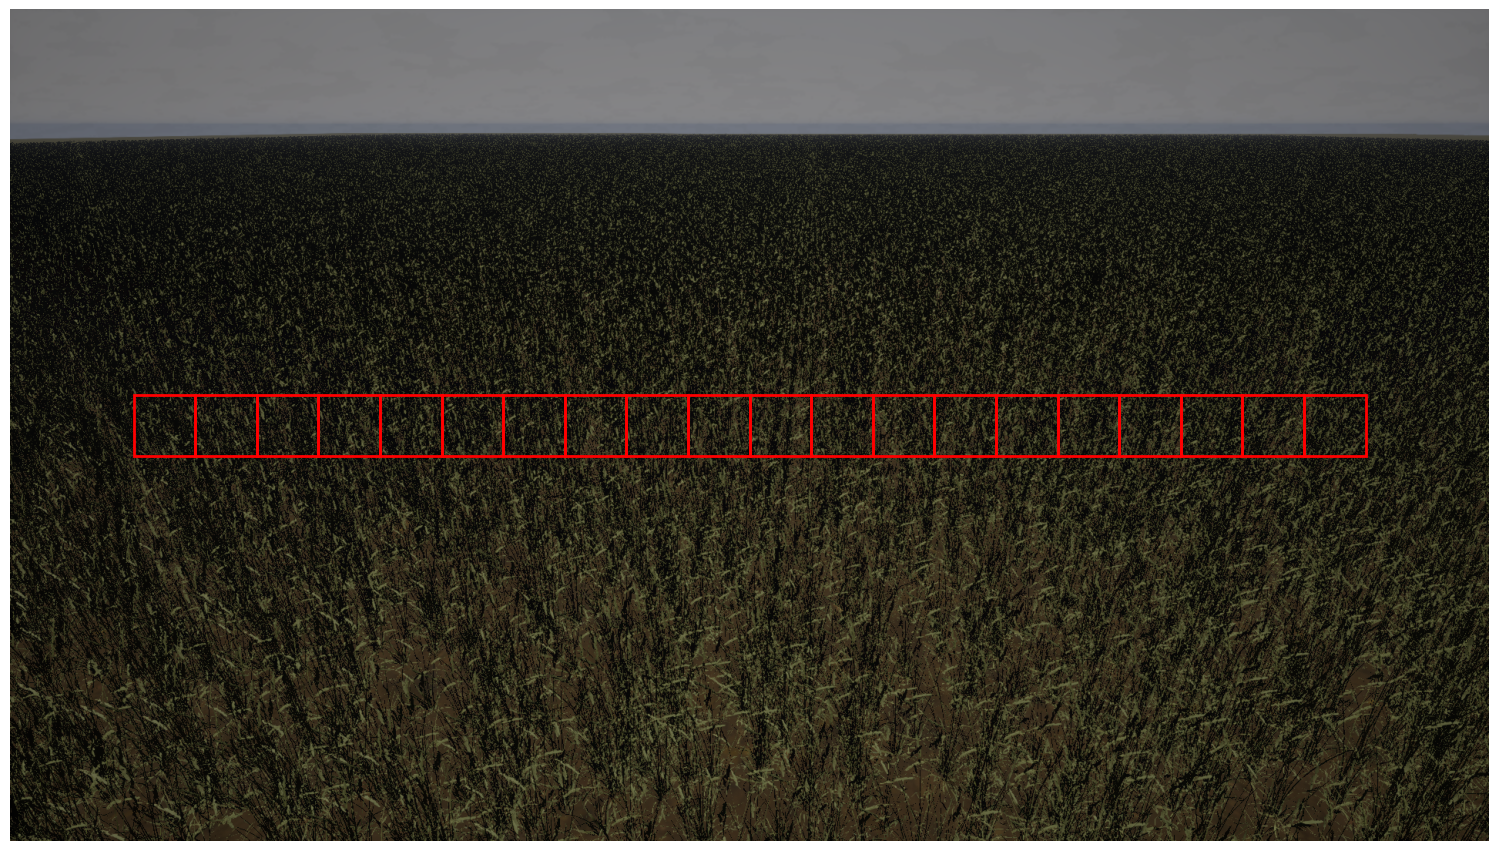
\includegraphics[width=\linewidth]{images/12_img_08GRVI.png}
        \caption{Inherent GRVI = 0.08}
        \label{08}
    \end{subfigure}
    \hfill
    \begin{subfigure}{0.3\textwidth}
        \centering
        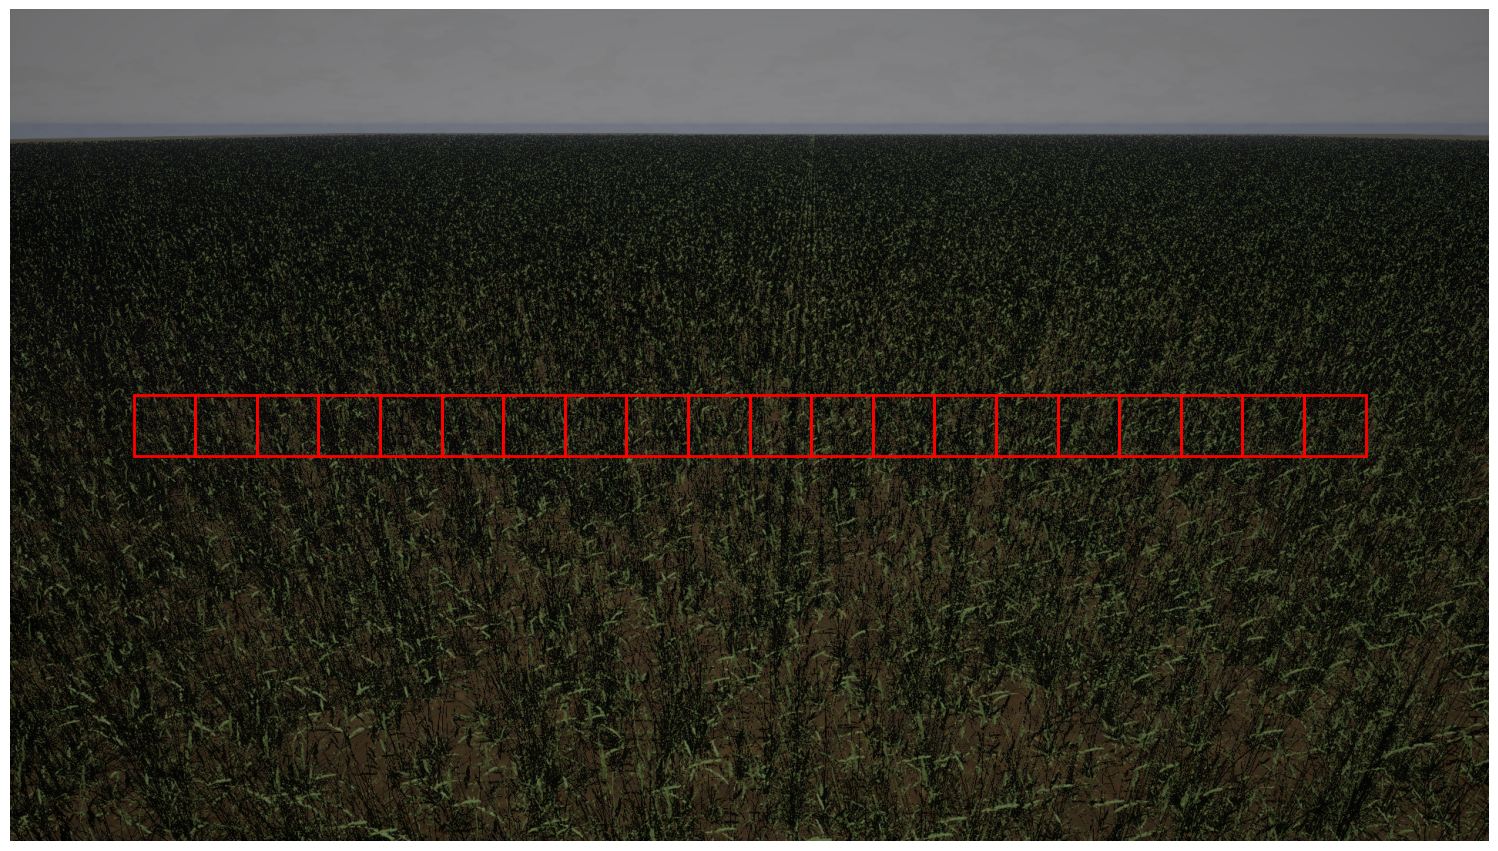
\includegraphics[width=\linewidth]{images/12_img_24GRVI.png}
        \caption{Inherent GRVI = 0.24}
        \label{24}
    \end{subfigure}
    \hfill
    \begin{subfigure}{0.3\textwidth}
        \centering
        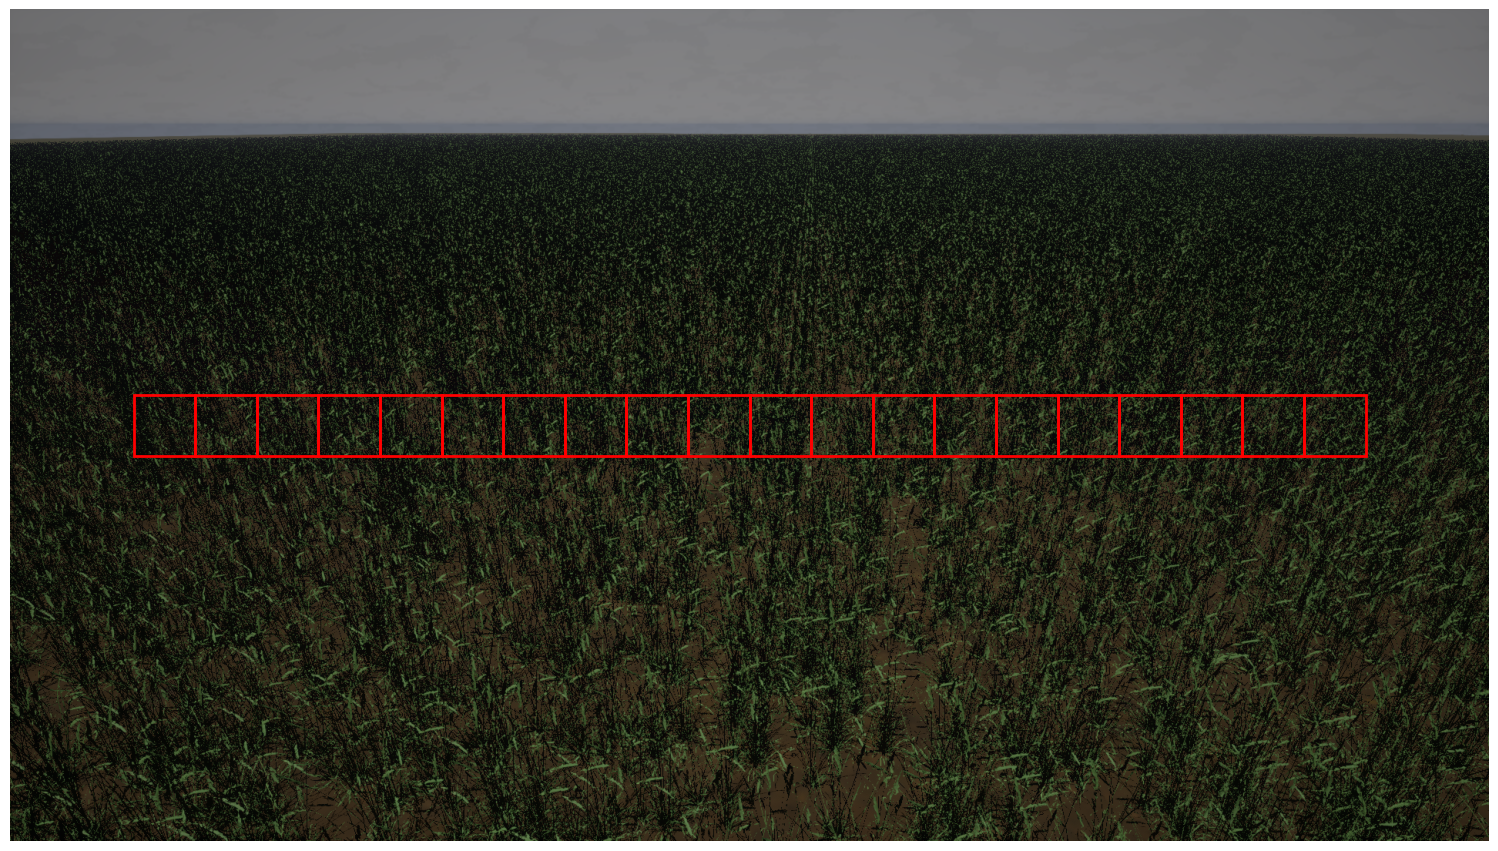
\includegraphics[width=\linewidth]{images/12_img_38GRVI.png}
        \caption{Inherent GRVI = 0.38}
        \label{38}
    \end{subfigure}

    \vspace{0.5cm}

    \begin{subfigure}{0.3\textwidth}
        \centering
        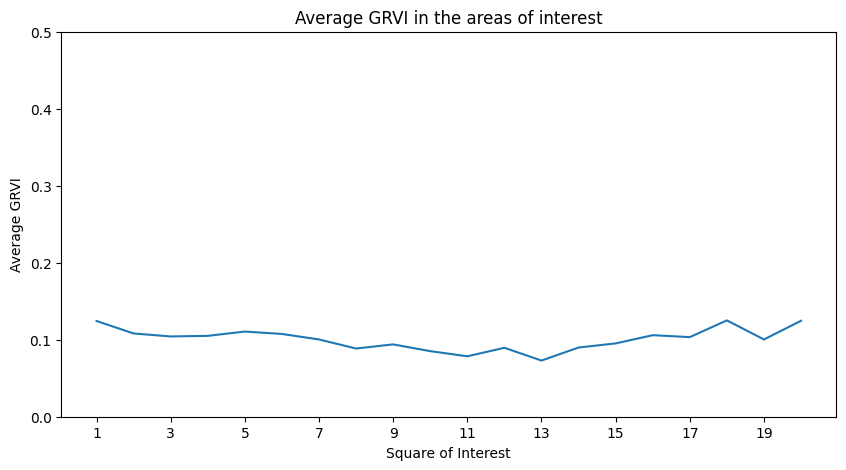
\includegraphics[width=\linewidth]{images/12_graph_08GRVI.png}
        \caption{Inherent GRVI = 0.08}
        \label{08diag}
    \end{subfigure}
    \hfill
    \begin{subfigure}{0.3\textwidth}
        \centering
        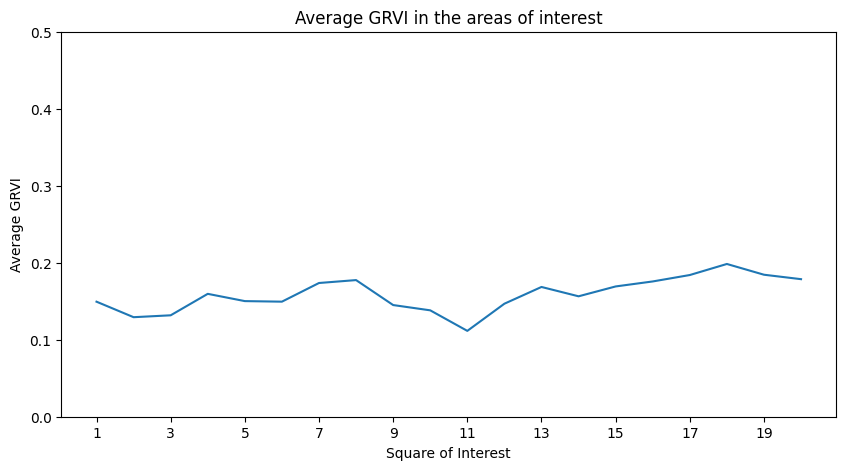
\includegraphics[width=\linewidth]{images/12_graph_24GRVI.png}
        \caption{Inherent GRVI = 0.24}
        \label{24diag}
    \end{subfigure}
    \hfill
    \begin{subfigure}{0.3\textwidth}
        \centering
        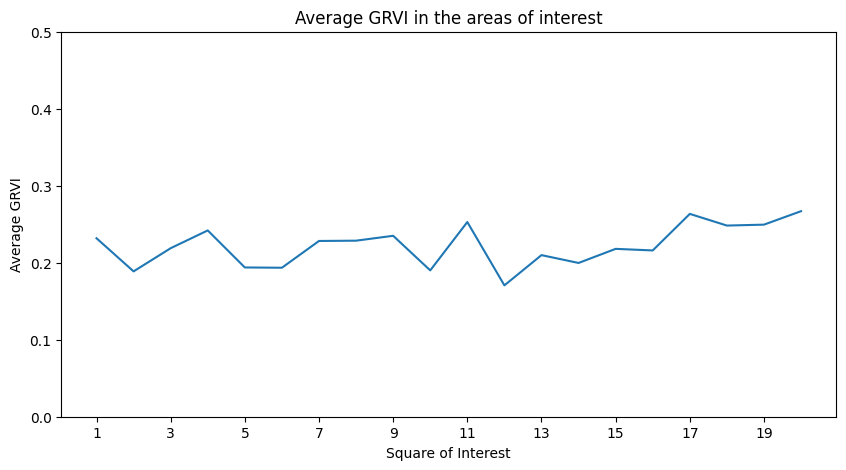
\includegraphics[width=\linewidth]{images/12_graph_38GRVI.png}
        \caption{Inherent GRVI = 0.38}
        \label{38diag}
    \end{subfigure}

    \caption{Images captured under overcast lighting conditions, with SZA fixed at $20^\circ$. The red squares indicate the bounds of the areas-of-interest. The corresponding graphs present the mean calculated GRVI within the individual area-of-interest. The material used for the illustrated plants has an inherent GRVI of 0.08, 0.24 and 0.38, respectively.}
    \label{cloudy-grid}
\end{figure}

The first observation made while reviewing the GRVI per area-of-interest graphs was the susceptibility of different materials to the various sources of error. Particularly, line graphs depicting GRVI values calculated while a high inherent GRVI material is applied appear more jagged, with large dips where planting is not as dense and soil is more visible. On the other hand, line graphs associated with lower GRVI materials appear to be smoother. However, they have a subtle trend towards the frames' edges, implying higher susceptibility to vignetting, caused by lens geometry and light falloff, an effect not as prominent for higher GRVI materials.

Secondly, by reviewing the graphs, a concerning observation regarded the discreteness of different GRVI values, as they are calculated from the collected data. As mentioned before, I have developed $16$ instances of the same material, with their inherent GRVI values ranging from $0.08$ to $0.38$, with a $0.02$ step. As illustrated in Figure~\ref{cloudy-grid}, the range of average GRVI values calculated from data collected under cloudy conditions per material is condensed to $\begin{bmatrix}0.1, & 0.22 \end{bmatrix}$, with the standard deviation of the highest GRVI material for the specific sample being almost $0.029$. That means, that there is potential overlap between different materials' measured GRVI. This motivated me to use all the frames collected during the dummy sequences' executions in order to calculate the average GRVI per material, as that appears in the scene, effectively mapping the inherent value of the material with how it is perceived. The results are presented in Table~\ref{grvi_stats}.


\begin{table}[htb]
    \centering
    \caption{Calculated mean GRVI and standard deviation for different inherent GRVI values.}
    \label{grvi_stats}
    \renewcommand{\arraystretch}{1.15}
    \begin{tabular}{c!{\vrule width 1.2pt}cc}
        \hline
        \textbf{Inherent GRVI} & \textbf{Calculated mean GRVI} & \textbf{Standard deviation} \\
        \hline
        \textbf{0.08} & 0.10066 & 0.01408 \\
        \textbf{0.10} & 0.10659 & 0.01422 \\
        \textbf{0.12} & 0.11679 & 0.01303 \\
        \textbf{0.14} & 0.12733 & 0.01587 \\
        \textbf{0.16} & 0.12052 & 0.01520 \\
        \textbf{0.18} & 0.12764 & 0.02197 \\
        \textbf{0.20} & 0.13732 & 0.02435 \\
        \textbf{0.22} & 0.13737 & 0.01772 \\
        \textbf{0.24} & 0.15887 & 0.02141 \\
        \textbf{0.26} & 0.16545 & 0.01875 \\
        \textbf{0.28} & 0.17287 & 0.02794 \\
        \textbf{0.30} & 0.18425 & 0.01657 \\
        \textbf{0.32} & 0.19349 & 0.02847 \\
        \textbf{0.34} & 0.19938 & 0.03181 \\
        \textbf{0.36} & 0.21248 & 0.02474 \\
        \textbf{0.38} & 0.22228 & 0.02641 \\
        \hline
    \end{tabular}
\end{table}

Table~\ref{grvi_stats} validates the previously expressed concerns. Although every inherent GRVI value maps to a calculated mean value, and both sides follow an upward trend - with the only outlier being the inherent value $0.16$, whose associated calculated value is lower than the one associated with the inherent value $0.14$ - the standard deviation of the calculations is relatively high, causing overlapping perceived GRVI values between different inherent values. It is also validated that the standard deviation tends to be higher for materials with relatively high inherent GRVI. 

As mentioned in the beginning of the \hyperref[datasssessment]{Data Assessment} section, dummy render sequences have been performed while a higher planting density was applied to the simulated field. For the assessment of the target values, it was important that I perform the same tests for the materials, as they appear during data collection. To achieve this, I identified which part of the field is depicted in every captured frame using the camera location data. For each frame, I calculated the average GRVI value of all the areas-of-interest depicting the same parts of the field, considering that in many captured frames, more than one parts are included, each with different applied wheat material, along with the standard deviation. Finally, I calculated the mean of the each previously calculated average that corresponds to parts of the field with the same material applied, along with the mean standard deviation.

The results are presented in Table~\ref{grvi_stats_ld}. It can be seen that the more prominent appearance of soil made the calculated GRVI to be reduced to less than half of the values tracked during the dummy renders, compressing the values even further to the $\begin{bmatrix}0.03865, & 0.11580\end{bmatrix}$ range, again, with relatively high standard deviation. However, their structure is still reasonable, with the perceived GRVI averages increasing as the corresponding assigned GRVI increases for almost all the cases.  

\begin{table}[htb]
    \centering
    \caption{Calculated mean GRVI and standard deviation for different inherent GRVI values.}
    \label{grvi_stats_ld}
    \renewcommand{\arraystretch}{1.15}
    \begin{tabular}{c!{\vrule width 1.2pt}cc}
        \hline
        \textbf{Inherent GRVI} & \textbf{Calculated mean GRVI} & \textbf{Standard deviation} \\
        \hline
        \textbf{0.08} & 0.03865 & 0.01138 \\
        \textbf{0.10} & 0.05840 & 0.01201 \\
        \textbf{0.12} & 0.05827 & 0.01102 \\
        \textbf{0.14} & 0.06596 & 0.01216 \\
        \textbf{0.16} & 0.06829 & 0.00959 \\
        \textbf{0.18} & 0.07512 & 0.01113 \\
        \textbf{0.20} & 0.08219 & 0.01363 \\
        \textbf{0.22} & 0.08231 & 0.01534 \\
        \textbf{0.24} & 0.08663 & 0.01367 \\
        \textbf{0.26} & 0.09405 & 0.01426 \\
        \textbf{0.28} & 0.10152 & 0.01515 \\
        \textbf{0.30} & 0.09916 & 0.01549 \\
        \textbf{0.32} & 0.10949 & 0.01665 \\
        \textbf{0.34} & 0.11360 & 0.01665 \\
        \textbf{0.36} & 0.11525 & 0.01743 \\
        \textbf{0.38} & 0.11580 & 0.01866 \\
        \hline
    \end{tabular}
\end{table}

Both in the cases of dummy and final renders, the calculated means of GRVI show the general behavior of the perceived GRVI, as the applied material instance changes. As mentioned before though, the fluctuations of the perceived values, hinted through the standard deviation, are averaged out. These fluctuations prevent us from simply mapping the average perceived values to the assigned GRVI of each material, due to the value overlaps they cause. To understand better the degree of overlap between the perceived values that correspond to different inherent values, I constructed a perceived GRVI map, where each presented value is the average perceived GRVI value for the corresponding part of the field. This map was the compared to the map of the field that presents the inherent GRVI values. The two maps are illustrated in Figure~\ref{grvi-maps}. 

\begin{figure}[htb]
    \centering
    
    \begin{subfigure}{0.48\linewidth}
        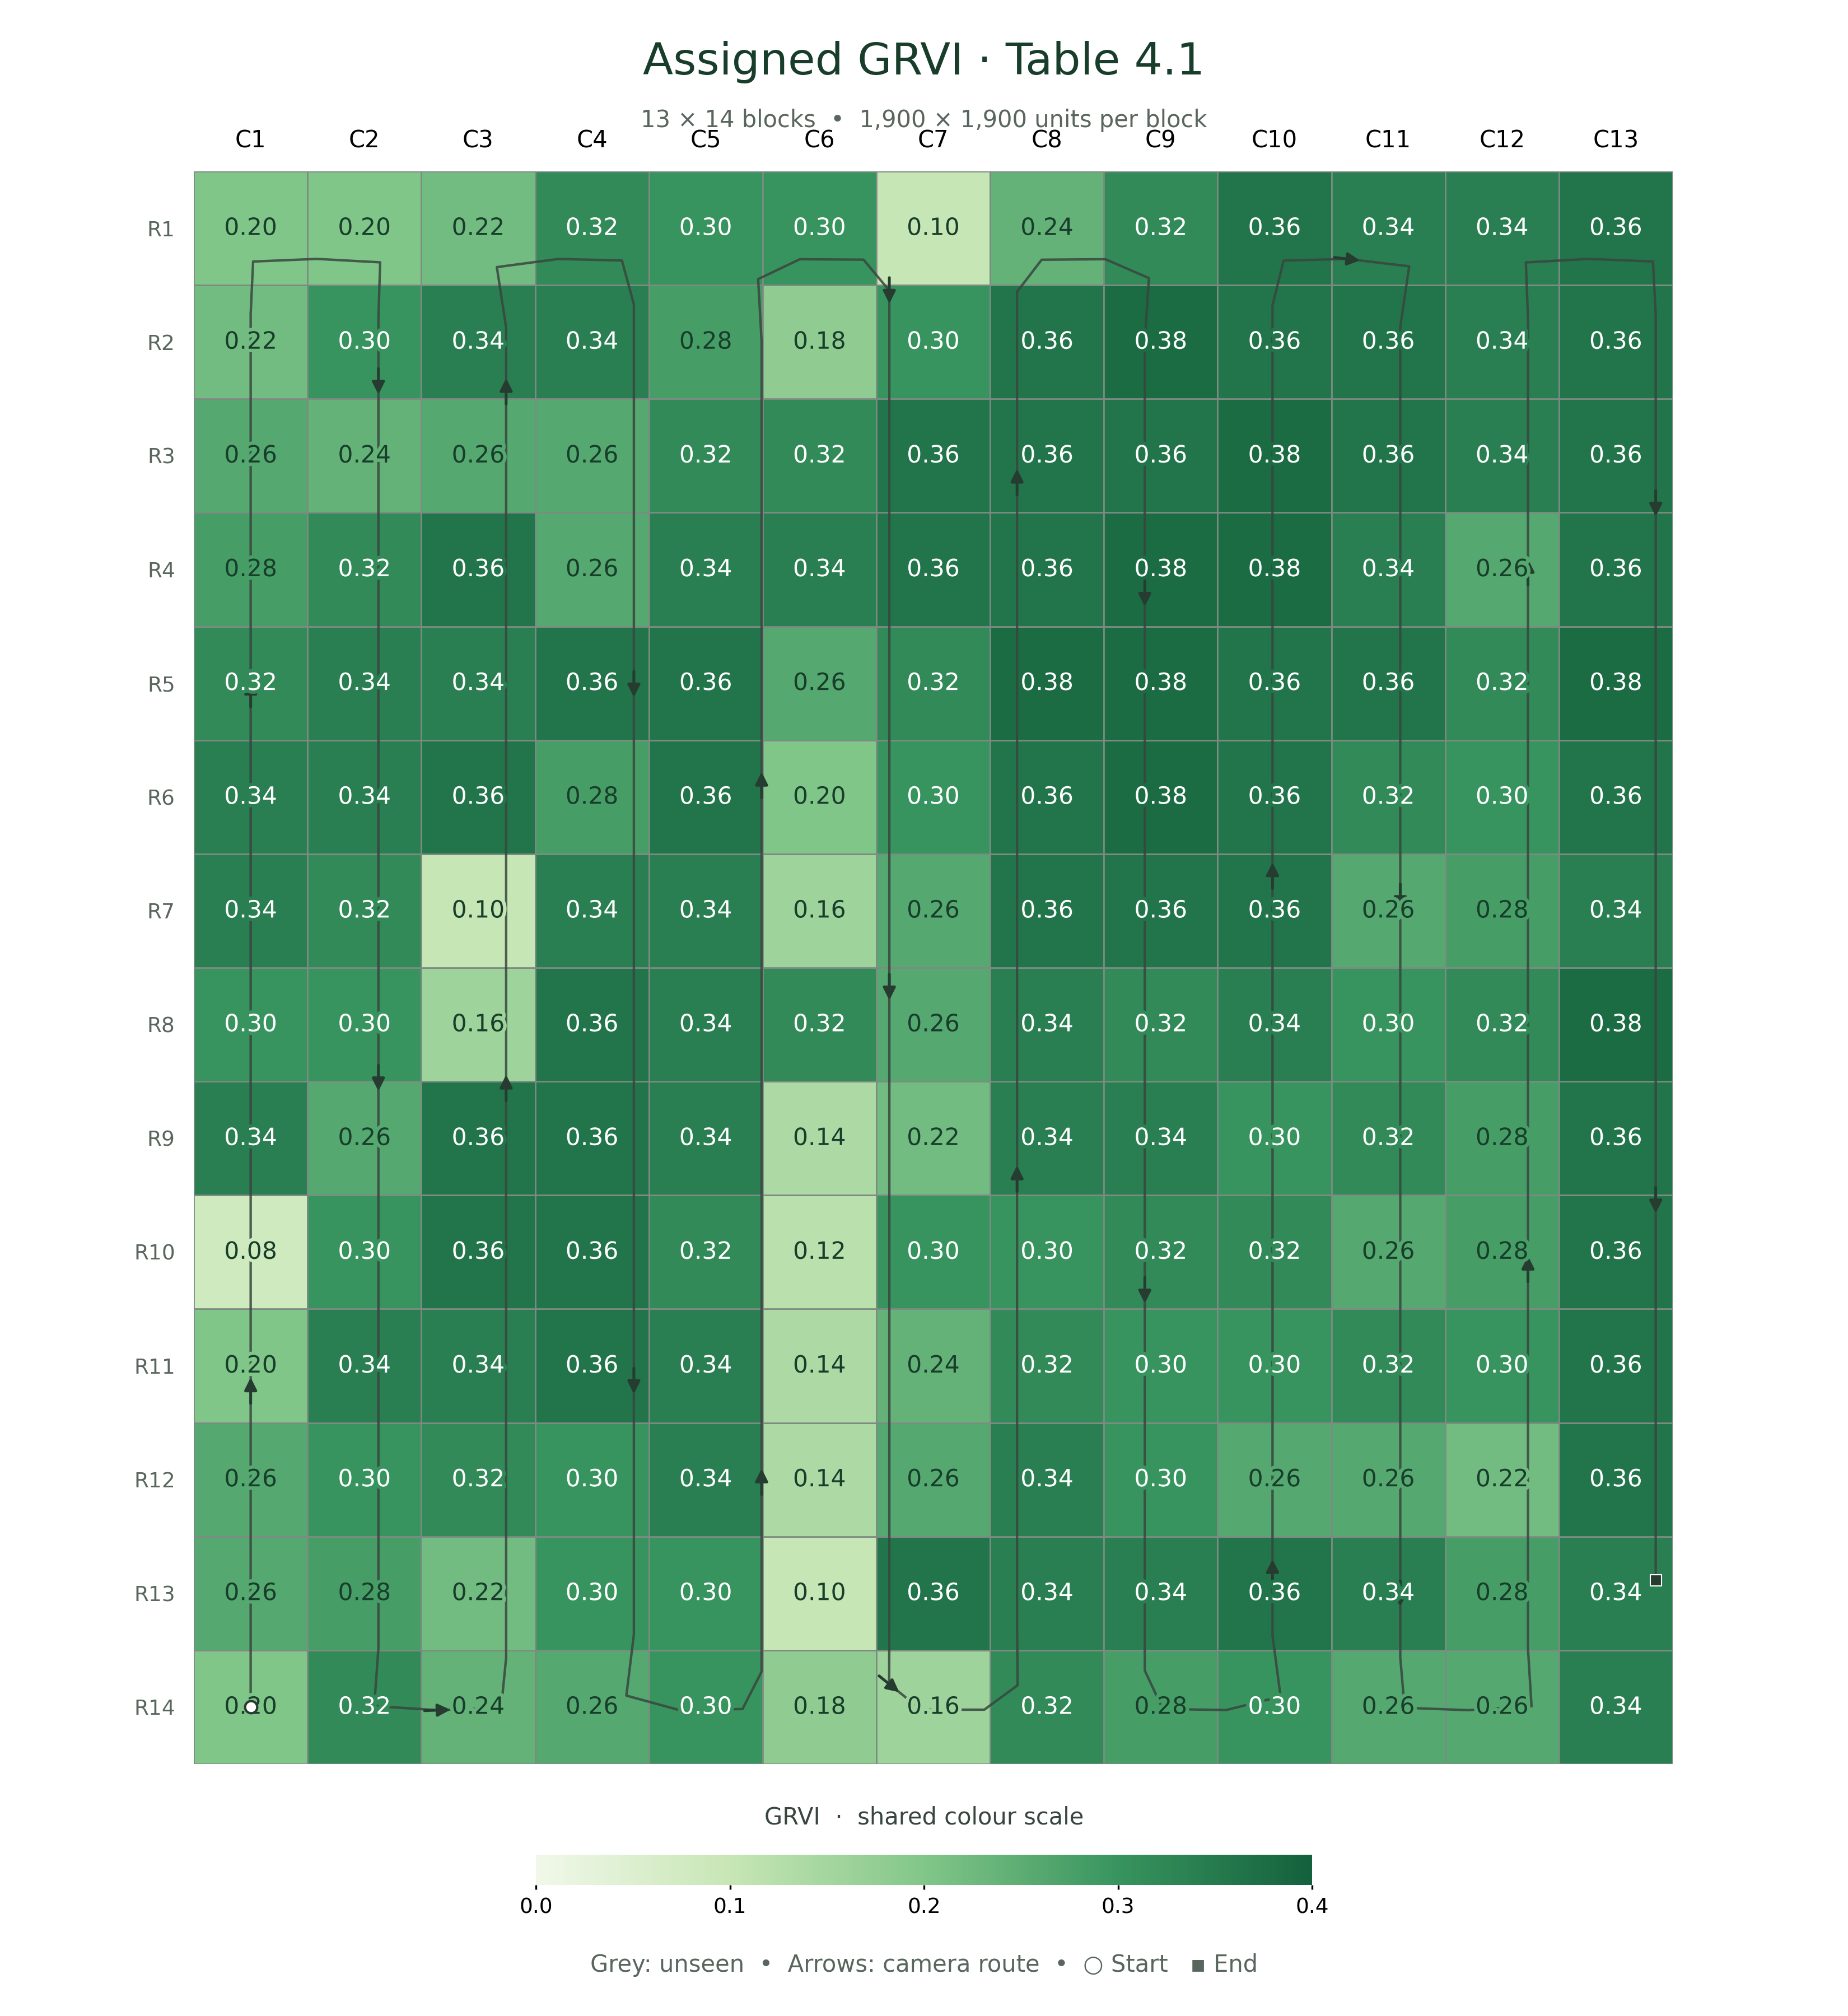
\includegraphics[width=\linewidth]{images/assigned_grvi_map.png}
        \caption{Map of assigned GRVI values per part of the field.}
        \label{assigned-map}
    \end{subfigure}\hfill
    \begin{subfigure}{0.48\linewidth}
        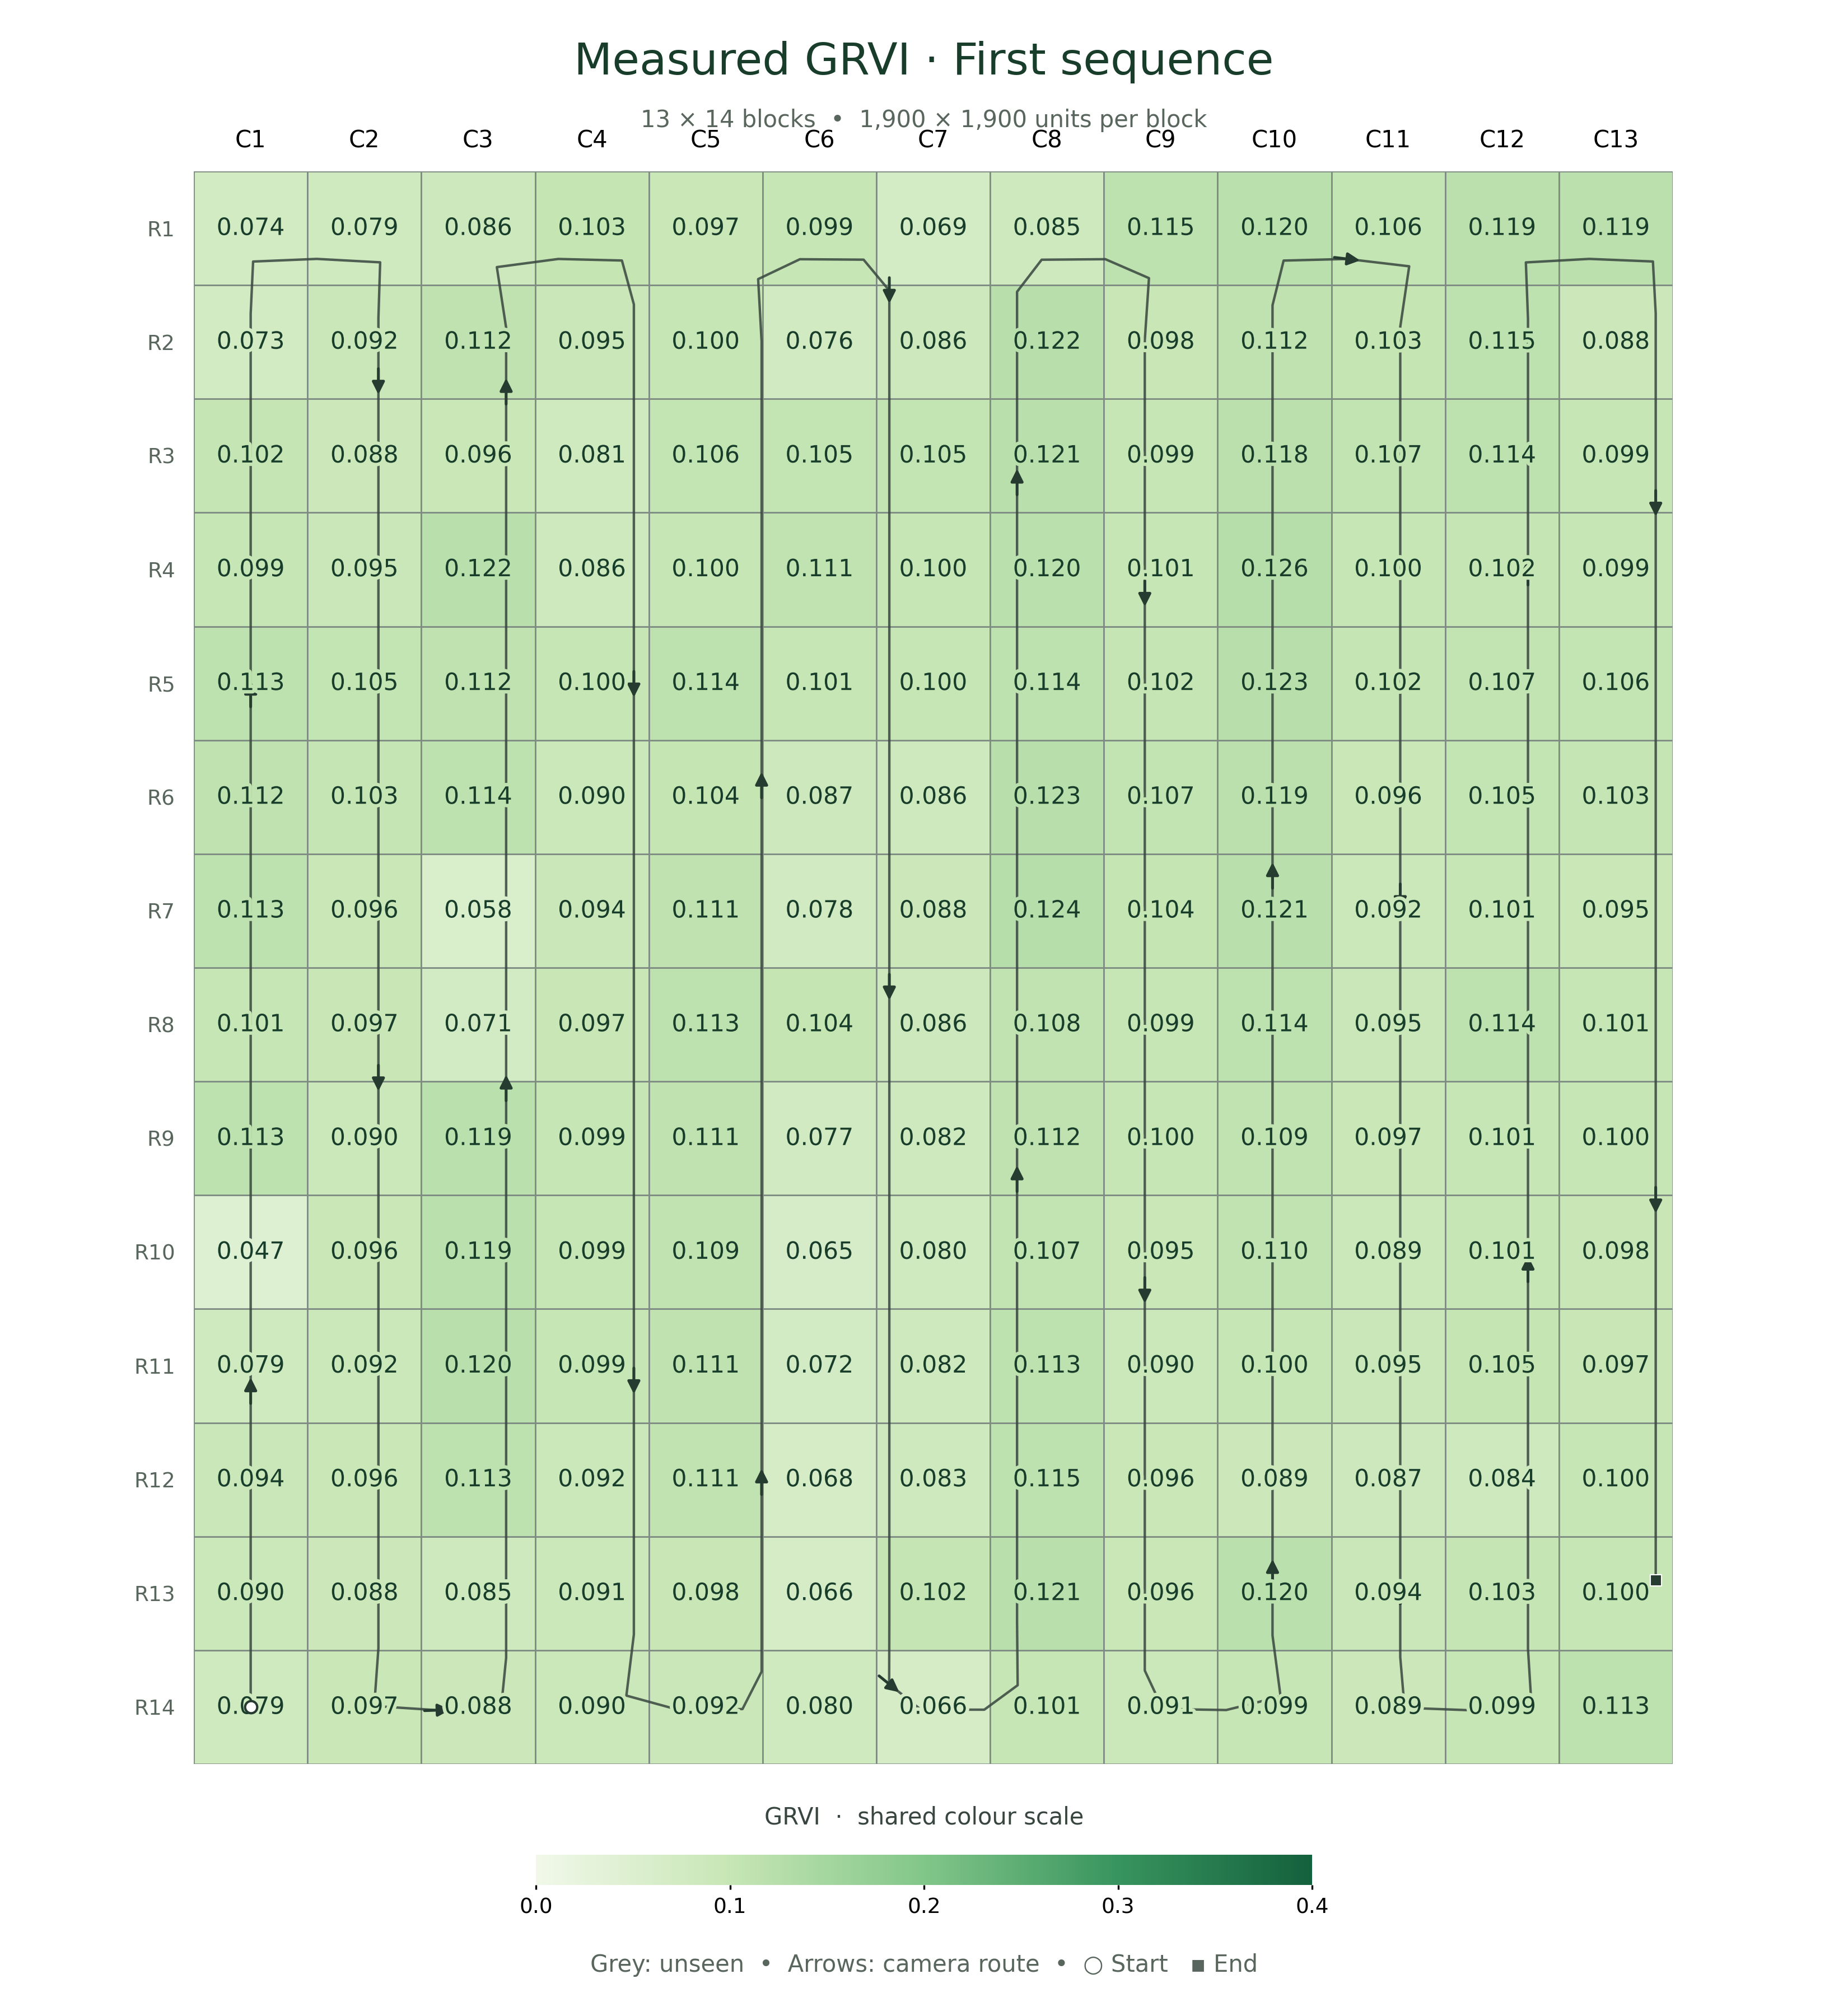
\includegraphics[width=\linewidth]{images/measured_grvi_map.png}
        \caption{Map of measured GRVI values per part of the field.}
        \label{measured-map}
    \end{subfigure}
    
    \caption{Both assigned and measured GRVI maps of the field. The arrows indicate the path the camera follows during data collection.}
    \label{grvi-maps}
\end{figure}

With multiple multiple cases of overlapping measured GRVI values between parts of the field with different materials assigned, I doubted whether using these values in their raw form is meaningful. An application that also accounts for factors other than the reflectance of the plants' surface could benefit from them. On any other case, using either directly the assigned GRVI or the measured GRVI averages, whichever achieves higher predictive performance, should be more beneficial.

In parallel with the investigation of the degree of overlap, I performed clustering on the measured values. The objective was to uncover whether it is reasonable to expect the measured values to be divided into $16$ groups, as many as the developed material instances. Specifically, as a first step, I re-used the average perceived GRVI of the areas-of-interest in each captured frame, previously calculated in order to construct the map illustrated in Figure~\ref{measured-map}. Next, I performed K-Means clustering using the calculated averages as inputs. All numbers of clusters between $2$ and $16$ were tested. Several of the results are illustrated in Figure~\ref{kmeans}.

\begin{figure} [htb]
    \centering
    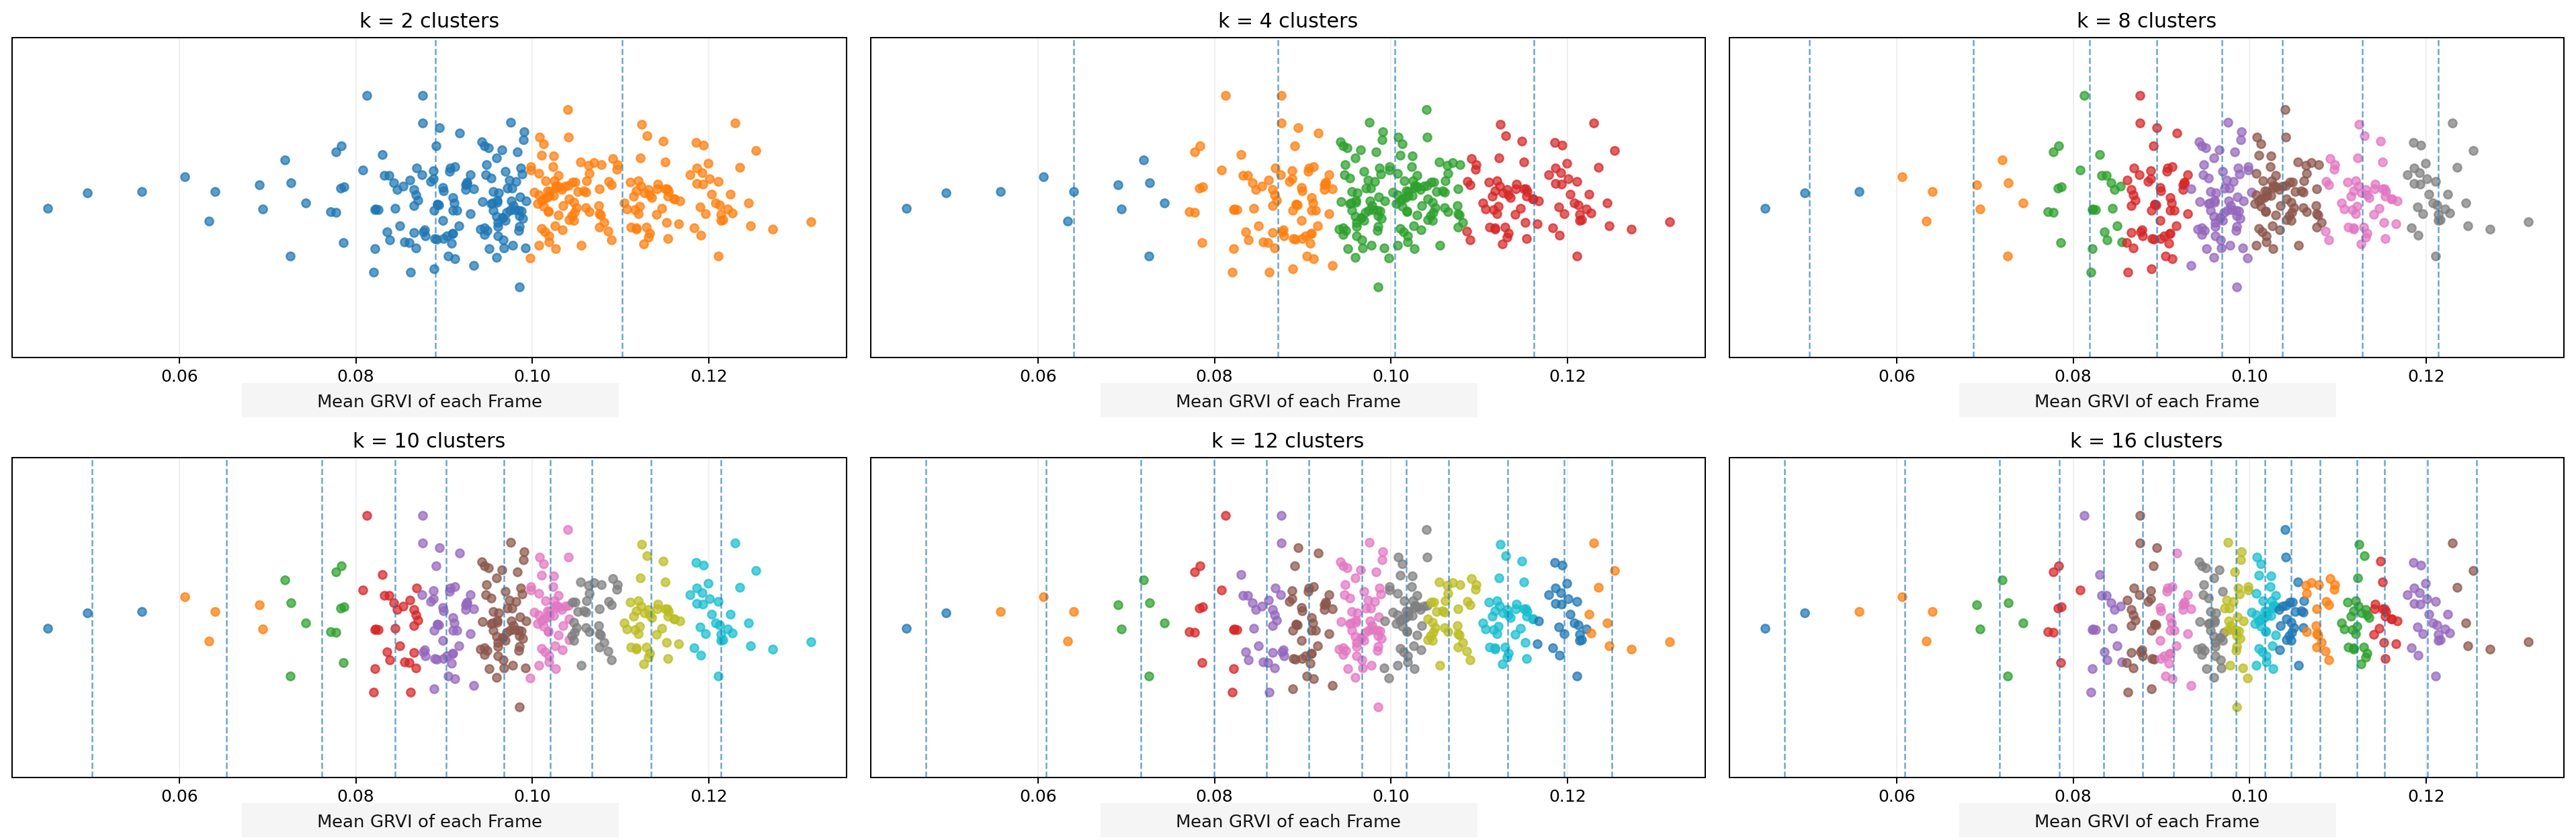
\includegraphics[width=1\linewidth]{images/cloudy-clusters.png}
    \caption{K-Means clustering performed with the average GRVI per frame as inputs, for different amounts of clusters. Random vertical offset was applied to the different points for clearer demonstration.}
    \label{kmeans}
\end{figure}

Using silhouette score as the primary evaluation metric, the results for different amounts of clusters were relatively close. Specifically, a silhouette score higher than $0.53$ was achieved for all the amounts of clusters tested, with the highest score being $0.562$ for four clusters. For $16$ clusters, being the ideal amount since it matches the amount of materials, the achieved score was $0.542$. Although $16$ clusters did not provide a separation as coarse as $4$, it was still considered as a viable option, due to the minimal loss of clustering quality. 

\subsection{GRVI Affected by Shadows}
\label{shadows-aff-grvi}


Shadows are also expected to affect the calculations of the perceived GRVI values. I found it therefore necessary to investigate the degree at which this occurs, examining whether it is actually meaningful to include shadows to the error factors the proposed models aim to address. All the tests were performed using data collected during the final render sequences.

The first conducted experiment aimed to check how the GRVI of different materials is perceived in shaded parts of the field. Having performed data data collection beforehand, I selected the samples captured while the absolute value of SZA was set to $85^\circ$ and calculated the average perceived GRVI per different material. I chose to use the absolute value rather than either the positive or negative, since in both cases, green- and red-band illuminance is the same but, the areas that are shaded in one case are not shaded in the other. That means that, if only one SZA was selected, some materials would not appear shaded, and metrics would not be extracted. 

The results are presented in Table~\ref{grvi_stats_gloomy}. Despite the expected upward trend of the calculated means as the assigned values increase, there were several concerning observations. For starters, the standard deviation is particularly high, indicating a high degree of variance between the samples. The monotonicity is also interrupted in more points compared to the values presented in the diffuse lighting section. Finally, this is the first case in which negative GRVI values are observed. 


\begin{table}[htb]
    \centering
    \caption{Calculated mean GRVI and standard deviation for different inherent GRVI values for frames depicting shaded scenes. SZA was set to $\pm 85^\circ$.}
    \label{grvi_stats_gloomy}
    \renewcommand{\arraystretch}{1.15}
    \begin{tabular}{c!{\vrule width 1.2pt}cc}
        \hline
        \textbf{Inherent GRVI} & \textbf{Calculated mean GRVI} & \textbf{Standard deviation} \\
        \hline
        \textbf{0.08} & -0.07121 & 0.06419 \\
        \textbf{0.10} & -0.01105 & 0.16058 \\
        \textbf{0.12} & -0.00470 & 0.07888 \\
        \textbf{0.14} & 0.02134 & 0.09981 \\
        \textbf{0.16} & 0.04428 & 0.08928 \\
        \textbf{0.18} & -0.13216 & 0.07311 \\
        \textbf{0.20} & 0.01871 & 0.09108 \\
        \textbf{0.22} & 0.05434 & 0.09088 \\
        \textbf{0.24} & 0.06008 & 0.10230 \\
        \textbf{0.26} & 0.07818 & 0.07561 \\
        \textbf{0.28} & 0.06839 & 0.08143 \\
        \textbf{0.30} & 0.07080 & 0.08523 \\
        \textbf{0.32} & 0.10111 & 0.07727 \\
        \textbf{0.34} & 0.09300 & 0.07372 \\
        \textbf{0.36} & 0.11045 & 0.07813 \\
        \textbf{0.38} & 0.11496 & 0.07893 \\
        \hline
    \end{tabular}
\end{table}


Further inspection of both the raw frames and the extracted data helped with the identification of multiple contributing factors for the existence of both negative values and high degree of variance. These factors were introduced with the inclusion of shadows in the scene and were exceptionally difficult to address, since some of them are uncontrollable to a degree, while others require solutions that will harm the consistency of the dataset. One of them is the shadow's consistency, considering that the cast shadow is not the result of a solid material but rather is cast by the leaves and branches of the tree mesh, leaving bright spots or incomplete light blockage at several points. The presence of sources other than Directional Light also plays an important role. Since Directional Light is cut off, these parts of the field are illuminated by other mechanisms, including the Sky Light actor and Lumen, whose red-green balance is different than the Directional Light's, affecting the red and green illuminance values measured by the light meters. Other suspected factors are the presence of soil, sensor artifacts caused by low lighting and disproportionate changes between the illuminance values for each band and luminance values for each band.

It was unclear wether these factors affect the dataset as a whole or just create large amounts of outliers, harming the calculated mean values. In order to clarify this, I performed the Median Absolute Deviation (MAD) method in order to identify and exclude possible outliers. That said, even after excluding the detected outliers, there was no noticeable change in the calculated means.

It was also tested whether different SZA values affect the measured GRVI for a shaded area. Specifically, I randomly selected frames depicting shaded parts of the field, each having materials with different inherent GRVI values, and compared the average GRVI values measured within them with the averages calculated using frames of the same parts of the scene but with different set SZA values - naturally, for SZA values where the examined parts remain shaded. The measured values for three of the selected materials are illustrated in Figure~\ref{gloomy-diff-mats-and-sza}. It can be seen that the perceived GRVI of materials with high inherent GRVI increases as the absolute value of SZA increases, while the opposite happens for materials with low inherent GRVI. 


\begin{figure} [htb]
    \centering
    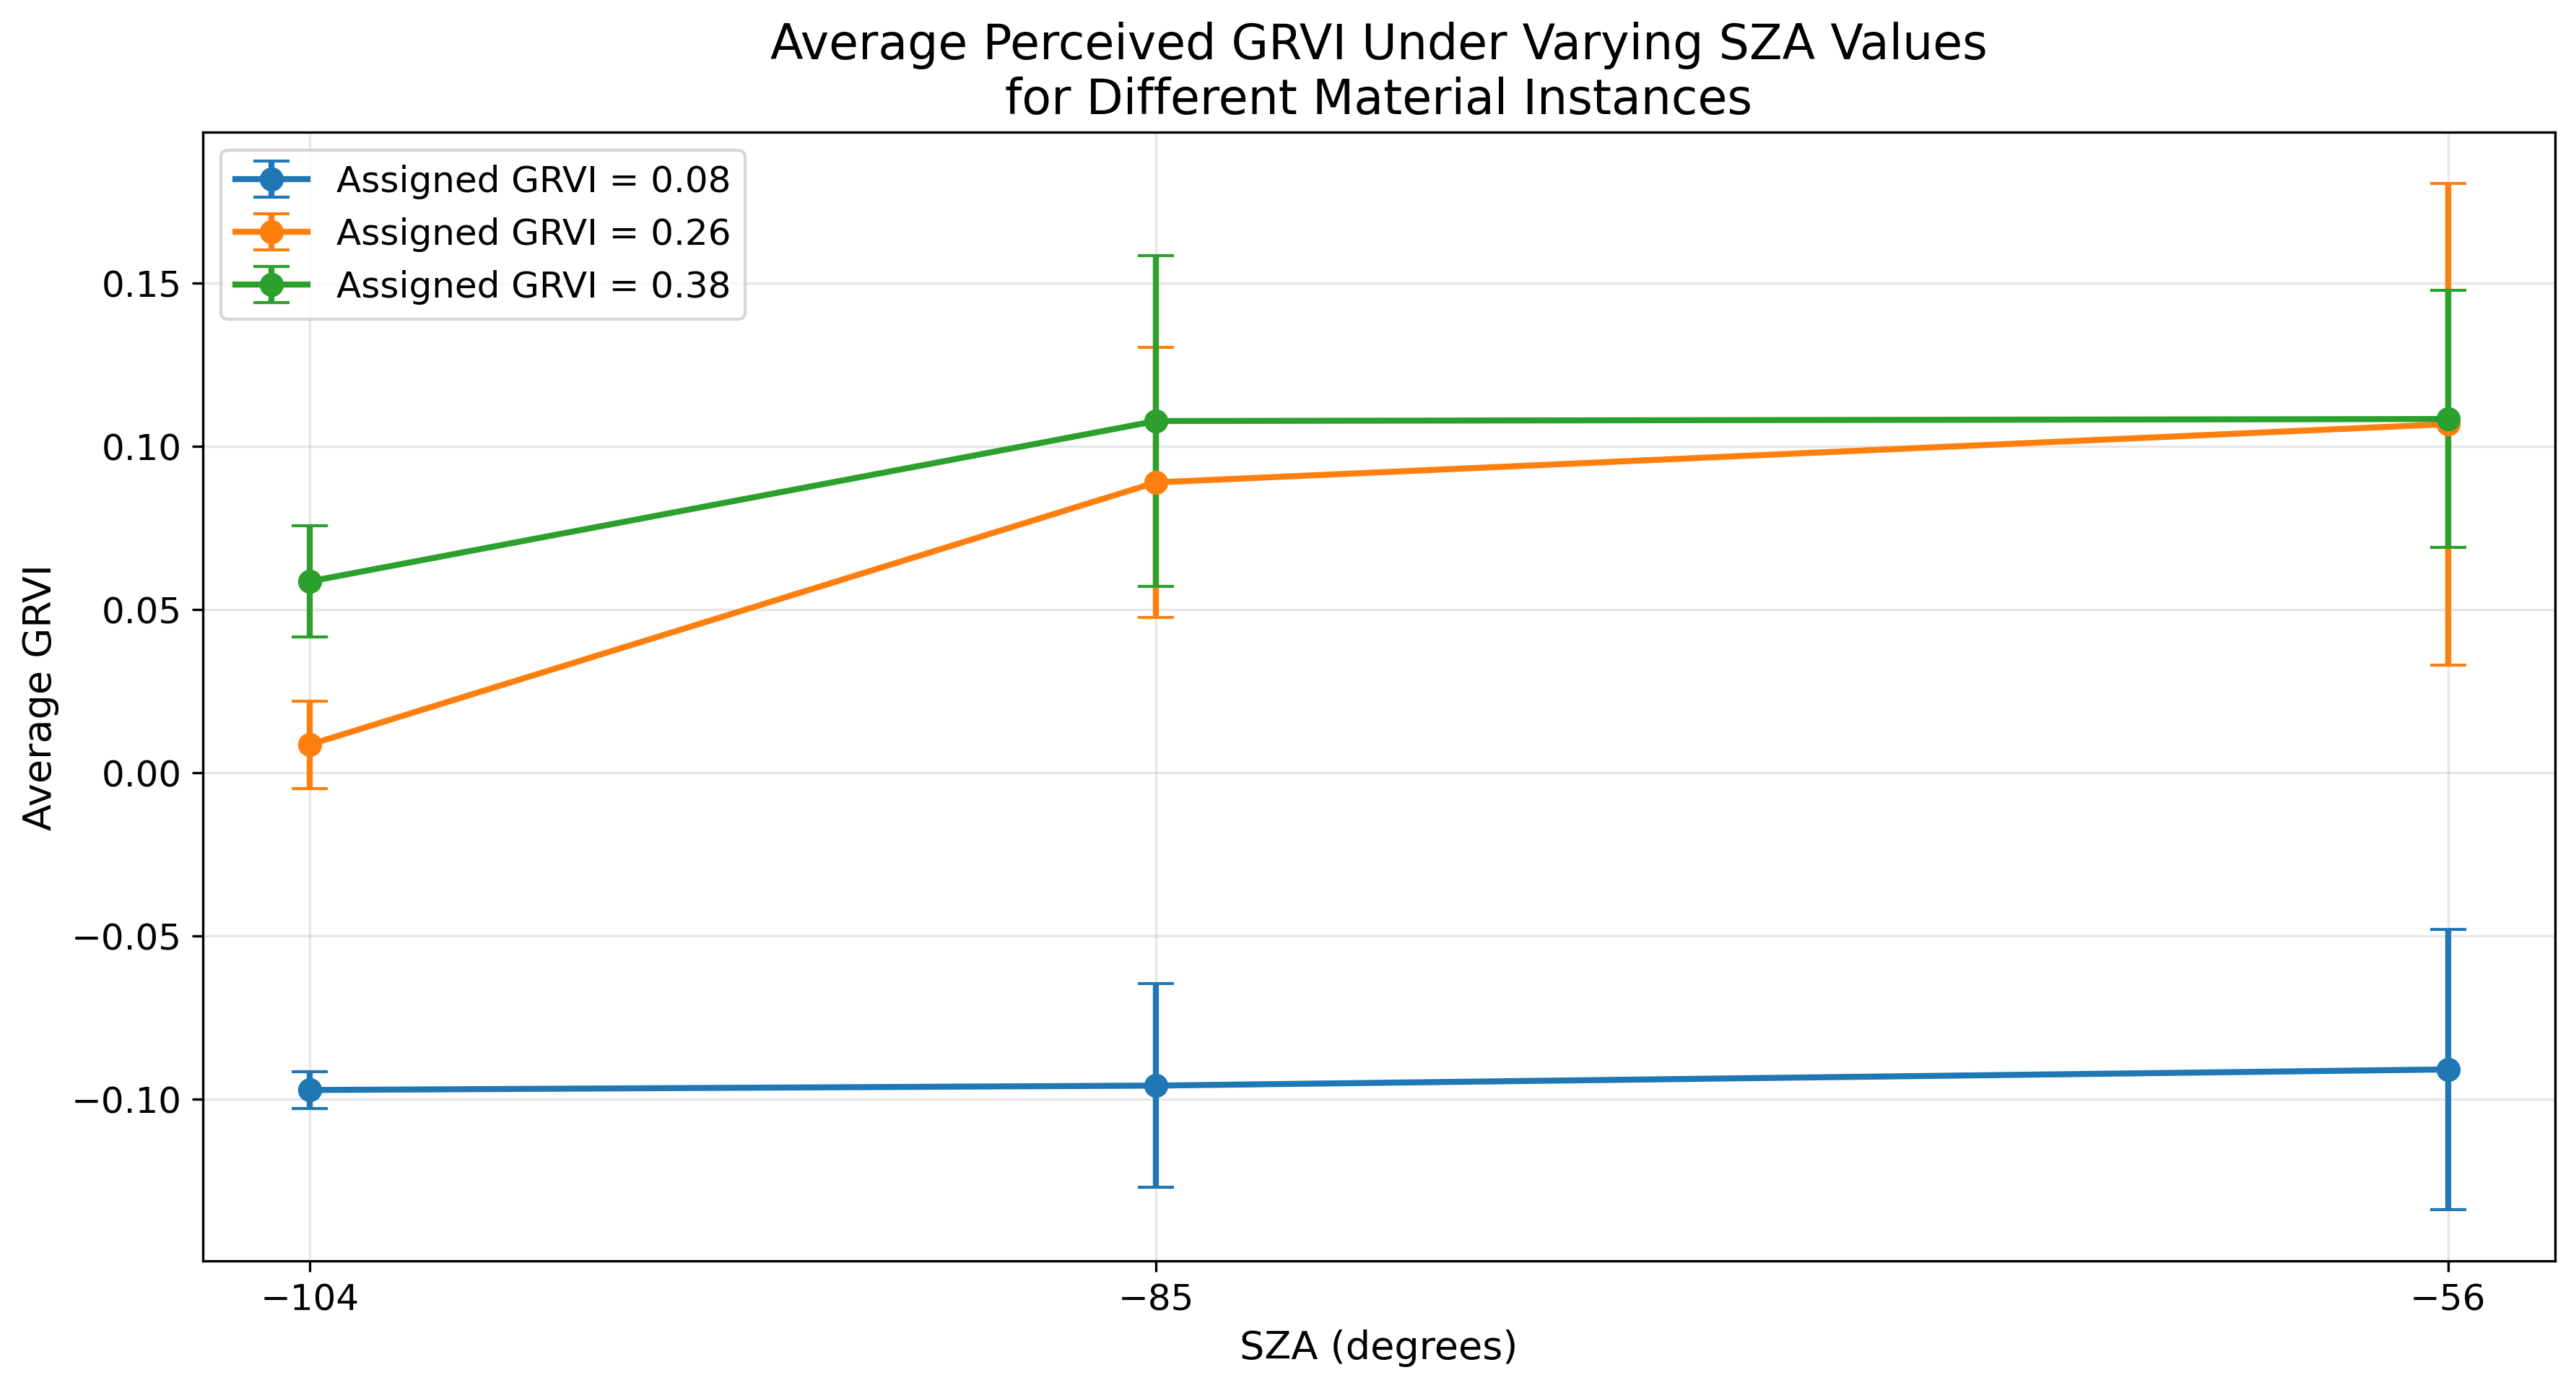
\includegraphics[width=1\linewidth]{images/grvi_vs_sza.png}
    \caption{Average perceived GRVI calculated for different SZA values and different materials. Vertical lines represent standard deviation.}
    \label{gloomy-diff-mats-and-sza}
\end{figure}

Overall, the findings suggest that the presence of shadows introduces significant distortions in the perceived GRVI values, affecting both their accuracy and consistency. The persistence of these deviations after outlier removal indicates that they cannot be attributed solely to isolated measurements, but rather reflect systematic effects associated with shaded conditions. Although the individual contribution of each identified factor remains difficult to isolate, the results demonstrate that shadows constitute an important source of GRVI measurement error and therefore justify their inclusion among the factors that the proposed correction models aim to address.


%note for later: REALLY need to find photos from the dataset with trees and shadows etc


\subsection{Front - Back}
!!!! some things about the front back thing + the grvi maps 



% Based on the problem they aim to tackle, there were two kinds of ML models developed. The first one aimed to tackle just the error introduced by the measuring media and conditions (the assumption of isotropic BDRF, non properly calibrated sensors, the variations caused by the different illumination scenarios etc.) and therefore was not trained to the half of the dataset that includes shadows. The second aimed to assess all sources of errors mentioned above, plus the inclusion of tree shadows.

%Another discrimination of the ML models that were developed regarded the selected ground truth. On the first case, four additional renders were performed, two for each render direction (start of spline to end of spline and the opposite). All four renders were performed under simulated overcast lighting, since overcast lighting eliminates the errors introduced by either BDRF anisotropy or shadows and all four were performed with a SZA of 20. Among the two renders corresponding to each direction, one was performed with a green-band illuminance of 322 and one with 1020, allowing the selection of the most suitable between the two (the criteria of the selection are analytically described in the next chapter). On the second case, the target GRVI of the models was the inherent GRVI of the material assigned to each plant mesh, with the estimation of which material was assigned to each depicted plant in the frame using the stored SCC coordinates.
    \chapter{Data Preprocessing and Feature Engineering}
\label{chap6}

So far, the data collected are:

\begin{itemize}
    \item the frames that were captured during the finalized render sequences, encapsulating the luminance reflected by the surfaces and reaching the SCC,
    \item the absolute rotation (in roll, pitch and yaw) and cartesian coordinates of the SCC inside the simulation, recorded for each frame captured,
    \item the absolute rotation (in roll, pitch and yaw) of the sun, recorded for each render sequence, with the roll angle being set equal to the the SZA throughout the experiment,
    \item the readings and absolute cartesian coordinates of the light meters and,
    \item the assigned GRVI value of the material applied to each area of the field.
\end{itemize}

Considering that, the algorithms selected to be trained for correcting the perceived GRVI values are mainly shallow Multi-Level Perceptrons and ensemble ML methods, this data should be structured in a way interpretable for them. The processed I followed for achieving that is described in this chapter.

\section{Data Preprocessing}
\label{dp}

Considering the nature of the ML models that were elected as ideal for this application, transforming the collected information into tabular data - data structured into rows and columns, much similar to a spreadsheet - seemed fairly intuitive. Ensemble methods in particular have historically performed strongly in classification and regression tasks with tabular data as inputs \cite{tabdata-gen}, while specially tuned NN architectures have begun to emerge for these applications \cite{tabnet, tabdata-nn}. 


In this study, each row corresponds to an area-of-interest extracted from the frames captured during the render sequences, while each column provides the information necessary for each area-of-interest. As a reminder, the areas-of-interest for which the GRVI values were calculated are twenty adjacent square regions arranged horizontally across the image, with their common vertical position being the vertical center of the frame (Figure~\ref{aoi}). Before any kind of feature engineering was performed, the data I decided to include as inputs for the trained algorithms were (along with their column names when stored in .csv files):

\begin{itemize}
    \item the average perceived GRVI value of the area-of-interest ($grviIn$),
    \item the average red and green reflectance of the area-of-interest ($meanRefR$ \& $meanRefG$),
    \item measured illuminance for the red and green bands, either unique to the sample or the render sequence (more on that later) ($illumR$ \& $illumG$),
    \item index of the area-of-interest within the frame it was extracted from (bolckIdx),
    \item roll, pitch and yaw of the sun ($sunRoll$, $sunPitch$ \& $sunYaw$),
    \item roll, pitch and yaw of the SCC ($camRoll$, $camPitch$, \& $camYaw$), and
    \item the target value ($grviOut$)
\end{itemize}

Other information that could be included in the inputs was the average red and green luminance of the area-of-interest, but I avoided it since, considering that the final objective is deployment on an edge device, redundancy would noticeably increase computational overhead. For the same reason, several of these features were removed later on. From the information mentioned in the introduction of this chapter, the SCC's location data were not included in order to avoid spoonfeeding the model, considering that it should perform while being agnostic to location. The light meters' location data were also not used as features since they did not provide meaningful information. However, both SCC's and light meters' coordinates were used during data preprocessing

Most of the aforementioned features were directly available for being structured into the desired format. The data associated with the measured reflectance of the studied surfaces and, consequently, GRVI, though, had to be drawn out from the captured frames and calculated using other contributing metrics.

\subsection{Calculating Input Reflectance and GRVI}

As mentioned in Section~\ref{photom-q-meas}, the reflectance of a surface is calculated using the reflectance formula for Lambertian surfaces:

\begin{equation}
    \rho_b = \frac{L_b \times \pi}{E_b}\,,
    \label{lambertian1}
\end{equation}

with $\rho_b, L_b$ and $E_b$ being the reflectance, luminance, and illuminance per band, respectively. Therefore, the calculation of reflectance can be separated into three stages: extracting luminance per band for the surfaces presented in the area-of-interest, acquiring the illuminance reaching these surfaces and eventually performing the calculation. 

To retain the luminance of the areas-of-interest, the captured images had to be read sequentially, maintaining the green- and red-channel values of the selected points in the process. The images were previously organized in a way that each of them belonging to a render sequence was stored in the same folder and indexed relative to the other images in the same sequence, based on the order they have been rendered. All the folders corresponding to render sequences were stored under a shared "home" folder. I developed a Python script that, given this "home" folder, it serially opens the folders existing within it, traversing through the frames they contain. Eventually, for each frame read, the script isolates the $20$ areas-of-interest and stores their red and green channels as NumPy arrays.

!!! present here folder architecture!!!

In order to use these arrays to calculate GRVI, the illuminance for each area-of-interest should also be known. As mentioned throughout this study, there were mainly three ways used for acquiring the illuminance of the scene: single stationary light meter, multiple light meters measuring the illuminance of the points included in the camera's field of view and single light meter attached to the same rig as the camera, measuring the illuminance near the camera. I used the first method in cases where there were no obstacles between the light source and the field's canopy. The light meter reading remained the same during each render sequence. I stored the measured value of each sequence in .txt files within the corresponding folder. This way, it was simple to use the same script that traverses through the captured frames to parse the illuminance values and, during calculations, use the appropriate one for each render sequence.

The second and third ways of measuring illuminance aimed to address the lack of robustness to illumination variability of the first. In the multiple light meter case, the readings and position of each sensor were stored in separate .txt files, again, residing within the corresponding render sequence folder. With five sensors deployed in the scene, there were five files created for each illumination scenario. Each row of the files refers to the respectively indexed frame, and contains information regarding four of its areas-of-interest. Consequently, the information found in all rows with the same index across the five files provides complete complete context for all the areas-of-interest of one frame. During the GRVI calculation, the Python script parses the light meter files and matches the readings with the appropriate frames based on their row index. For the single sensor approach, the illuminance readings corresponding to the central four areas-of-interest are used, captured during the multiple sensor approach. During GRVI, specifically while parsing the readings file, I shifted the readings to align the position of the camera and the sensor, matching each frame with the readings originally targeted for the previous.  The first frame and last sensor readings are discarded.

With the luminance of each area-of-interest represented as an array of pixel values and the corresponding illuminance measurements parsed, the next step was to calculate the red- and green-band reflectance of the depicted surfaces using Equation~\ref{lambertian1}. Both $\pi$ and the illuminance value were broadcast for multiplication and division with the luminance array. The red-band illuminance is used along with the red-band luminance, with the same process followed for the green-band measurements. The results are two arrays, each cell of which represents the reflectance of a tiny part of the captured surfaces in the respective bands. The average values of red- and green-band reflectance arrays were used as two of the features of the dataset.

Finally, the script calculates GRVI for every frame's areas-of-interest. Again, there are two possible approaches for calculating the average GRVI value of each cropped part of the frame. The first uses the calculated means of the reflectance arrays to output a single GRVI value (Equation~\ref{avgRefGrvi}). This method provided stable values with limited outliers, making it ideal for calculating the reference GRVI values using the frames collected under diffuse lighting conditions. The second approach was calculating GRVI using directly the red and green reflectance arrays (Equation~\ref{avgGRVI}). This results in a GRVI array containing a value for every pixel of the given area-of-interest. The mean of the array is then calculated and used as an input feature. The values produced using this method were particularly unstable, with multiple outliers, including measurements with absolute values greater than $1$, which is abnormal for a normalized index such as GRVI, whose values are capped in the $\begin{bmatrix}
    -1, & 1
\end{bmatrix}$ space. 

\begin{equation}
    GRVI = \frac{avg(\begin{bmatrix}RefG\end{bmatrix}) - avg(\begin{bmatrix}RefR\end{bmatrix})}{avg(\begin{bmatrix}RefG\end{bmatrix}) + avg(\begin{bmatrix}RefR\end{bmatrix})}
    \label{avgRefGrvi}
\end{equation}

\begin{equation}
    GRVI = avg(\begin{bmatrix}GRVImat\end{bmatrix}) = avg(\frac{\begin{bmatrix}RefG\end{bmatrix} - \begin{bmatrix}RefR\end{bmatrix}}{\begin{bmatrix}RefG\end{bmatrix} + \begin{bmatrix}RefR\end{bmatrix}})
    \label{avgGRVI}
\end{equation}

Both GRVI calculation methods display advantages and disadvantages when their output is used as input feature. The first provides stable values, but since the mean reflectance values in the two bands are already provided to the models, GRVI calculated using them is expected to provide limited additional information. The second method on the other hand, despite producing inaccurate values, could complement the context provided by the rest of the features. When it comes to the output GRVI, only the first method was used. As for the inputs, I created datasets using both methods, exploring the impact of each of them to the models' performance. 

The complete GRVI calculation pipeline is illustrated in Figure~\ref{PLaceHolder!!!!}.

\subsection{Create Datasets' Target Values}

With all the input features ready, the remaining task for the development of the datasets was the preparation of the target values. I created two kinds of datasets, regarding the type of the values the models were trained to approximate.

In the first kind, the target values were calculated using the perceived red- and green-band reflectance values, as they were perceived in the digital twin under diffuse lighting conditions. Using the frames rendered during the two sequences I performed for diffuse lighting conditions - one following the data-collection spline from its beginning to its end and one following the opposite route - and the version of the GRVI calculation pipeline described above, where the averages of the reflectance matrices are used, the result was two single column arrays, stored as .csv files. Each row represents the target GRVI value for each area-of-interest.

In the second, the target values were the ones I assigned to each material used. The crucial step in this case was identifying the parts of the field depicted in each frame, making possible the mapping of each area-of-interest with its inherent GRVI value. To perform this task, I developed another script that, using the camera coordinates during each frame-capture and given that the field is separated in $1.9m \times 1.9m$ parts, calculates which part (or parts) is depicted, and therefore which inherent material is present. Considering that, when a frame is captured in landscape orientation, a wide area is included in the final rendered image, there is always the possibility that more than one parts of the field are depicted. It was important that the script took account of this case and map different inherent GRVI values to each frame's areas-of-interest when needed. 

To do so, I had to estimate how the horizontal length of each area-of-interest maps into the digital twin. With the simplifying assumption that the SCC's simulated lens is not curved, I approximated the distance between the edges of leftmost and rightmost areas-of-interest to be $680$ centimeters within the simulation. Assuming also that that the counterpart of each area-of-interest in the digital twin has the same length as the others, the script is able to identify the bounds of each area-of-interest within the simulation and decide which part of the field each of them depicts, mapping eventually each of them to an inherent GRVI value. The pipeline for this process if illustrated in Figure~\ref{PlaceHolder!!!}. The results for both the beginning-to-end route and the opposite were saved in single column .csv files.

\subsection{Dataset Creation}
With the preparation of the average red- and green-band reflectance values and the perceived GRVI value for each frame's areas-of-interest, and both the labels based on measured and assigned GRVI values, all the data necessary for the models' training were available. The last step for creating the initial versions of the datasets was gathering all the data scattered across different files and folders and combining them in an easily interpretable by algorithms format.

The initial datasets I had decided to develop are:
\begin{itemize}
    \item Using as labels GRVI measurements under diffuse lighting conditions:
    \begin{enumerate}
        \item field without trees,
        \item field with trees - light meters ahead of camera,
        \item field with trees - light meters close to camera,
        \item 1. and 2. combined,
        \item 1. and 3. combined.
    \end{enumerate}
    \item Using as labels inherent GRVI values:
        \begin{enumerate}
        \item field without trees,
        \item field with trees - light meters ahead of camera,
        \item field with trees - light meters close to camera,
        \item 1. and 2. combined,
        \item 1. and 3. combined.
    \end{enumerate}
\end{itemize}

In all of the input samples, the sky is clear and the illumination scenarios are the ones presented in Table~\ref{ilmsce} (except GT conditions). The input features in all of the datasets are the ones presented in the beginning of section~\ref{dp}.

The selected method of storing the datasets was in .csv files. The Python script used for traversing the image folders and calculating the GRVI per area-of-interest was modified to handle the structuring of the data in this format. Specifically, every time the script accesses a render sequence folder, it creates an empty Pandas DataFrame object. As the program proceeds to open the contained frames and calculate the average perceived GRVI value for each of their areas-of-interest, the result, along with the rest of the features associated with it (mean calculated reflectance, index within frame, illuminance, sun and camera rotation) are stored as rows in the DataFrame. By the time all the images of a render sequence folder have been accessed, the DataFrame is stored on the hard drive as a .csv file containing information regarding only this sequence. I decided to first save the data for each render sequence separately because handling missing data and eventually matching inputs with target values was found to be simpler when working on a single sequence's data.

Post the creation of the files for the separate files, the remaining steps were adding the target value's column and combining the separate files into a complete dataset. I had already organized the target values in single column .csv files, correctly aligned with the indexing of the samples contained in the created files. That means that, by the time I developed a script that adds labels to the input features and combines them to a single dataset, adding the labels was as simple as assigning to the "grviOut" column of the DataFrame the target values column. I had developed the script with options on whether to traverse folders of scenarios with trees, without trees or both, and using or not the assigned GRVI values as ground truth. Eventually, all ten of the initially planned datasets were created.

\subsection{Alternative Datasets}

The initial datasets were meant to be used for training algorithms that consist of a single model. These architectures were expected to address all possible sources of error involved during the GRVI calculations, with the minimum degree of error possible. Another method I experimented with to minimize this error even further was training and combining different models designed to handle different sources of error into one hierarchical architecture, creating essentially a mixture of experts. This process required modifying the already existing datasets to be compatible with the training pipelines of each of the models included in the final system.

\subsubsection{Dataset for Shadow Detection Model Training}

One of the architectures I experimented with was a hard-gated mixture of experts, aiming to handle data acquired from shaded scenes differently than the rest. The key mechanism for choosing the appropriate model every time an input is given is a classifier responsible for identifying wether the shadow of a tree was present when a frame was collected. 

To train this classifier, a second version of the datasets that include trees had to be developed. Specifically, the originals' target values were the materials' ground truth GRVI values. For this task, the target values have to be binary labels, indicating wether the studied area-of-interest depicts shaded parts of the field not. Upon inspecting the data collected during the different render sequences, the common characteristic I found amongst all information captured while shadows were present was naturally the particularly low illuminance values, as they were measured by the light meters. This is caused due to the interference of the trees between the light meters and the light source.

For the datasets constructed using directly the collected data, identifying the images depicting shaded parts was as simple as comparing the associated measured green-band illuminance with a loosely defined threshold. This is possible since the lowest assigned green-band illuminance, featured in Table~\ref{ilmsce}, is $200$, while the illuminance measured in shaded parts is typically a single digit number, regardless the light source's intensity. By performing this comparison for all the samples, I added an additional column to these datasets, indicating whether there was a shadow present in the scene when the frame was taken, and whether the particular area-of-interest was within the occluded area.

Arguably, the addition of shadow-presence-indicating labels and training of ML models for the classification of shadows for these datasets is redundant. That said, it was mainly performed for later transferring these labels to the datasets constructed by shifting the central light meter's readings, simulating that a single light meter was mounted close to the camera. In these cases, the identification of shadows relies on more complex patterns within the data, since the light meter's readings could differ from the actual illuminance values near the studied area of difference. Eventually, I was able to directly transfer the labels calculated for the areas-of-interest from the dataset with the accurate light meters' readings to the rest of the datasets where shadows were present, since they are invariant to the light meters' positioning.

The result was the four original datasets which include data derived from shaded scenes, with an extra binary indicator. This indicator signifies whether the respective area of interest depicts a part of the scene that is occluded.

\section{Feature Engineering}
\label{feature-eng}

The initially created datasets aimed to provide a first idea of what is the predictive performance of the proposed ML models for this particular task. The next step was achieving a satisfying balance between predictive performance and computational efficiency. This task can be achieved with feature engineering. By performing feature engineering, it was possible to both reduce the dimensions of the original dataset and make the provided information more easily interpretable to the models.

This section aims to present the possible different feature engineering methods that I considered to employ for creating different version of the dataset, with the final goal being the aforementioned accuracy-compactness balance. The impact of each of these methods on these examined factors is discussed in the !!!! chapter !!!!.


\subsection{Dimensionality Reduction}

%% say stuff!!


\subsubsection{Feature Selection}
\label{feature-sel}

A common feature engineering practice is reducing dimensionality by dropping unimportant input attributes. An instance of such is low-variance features, being features that hardly change throughout the dataset. Another example is features that are strongly correlated with others. Finally, it is possible that one of the inputs simply does not provide any noticeable impact on the output's estimation.

When it comes to low-variance features, several can be directly identified by a quick dataset inspection. Specifically, $sunRoll$ and $camRoll$ remain the same and equal to $180$ and $0$, respectively, throughout all the examples, therefore were found safe to be removed. $camPitch$ was also expected to remain set to $-20$, but throughout the examples, the value seems to have subtle fluctuations. Therefore, I considered it better to run feature importance tests and validate its insignificance before dropping it.

Regarding correlated features, I found the Pearson Correlation Coefficient to be a fairly informative tool for identifying linear relationships between the features. I used it to construct correlation heatmaps for several of the previously mentioned versions of the dataset. However, the results among all tested iterations were expectedly close. One of the produced correlation maps is presented in Figure~\ref{correlation-hm}. The features $sunRoll$ and $camRoll$ remain constant throughout the dataset and therefore no coefficients were calculated between them and the other features. $illumG$ and $illumR$ are used for the calculations of $meanRefG$ and $meanRefR$, respectively, and therefore it is natural that they are correlated. Furthermore, throughout the simulation, as illuminance for one band grew, it grew for the other band as well, explaining why there is a strong relationship between them. It can also be seen that the perceived reflectance of each band follows the trend of the other band, while none of them is strongly correlated to $grviIn$. This is the case because. Lastly, $grivOut$ does not appear to be linearly related to any other feature. In a vacuum, that could be concerning, since $grviOut$ is expected to behave similarly to $grviIn$. That said, due to the infulence of directional light and shadows, $grviIn$'s values are expected to be unstable. Overall, it is seen later on that the models are able to learn the relationship between input features and the target values, implying the existence of non-linear relationships between them.

\begin{figure} [htb]
    \centering
    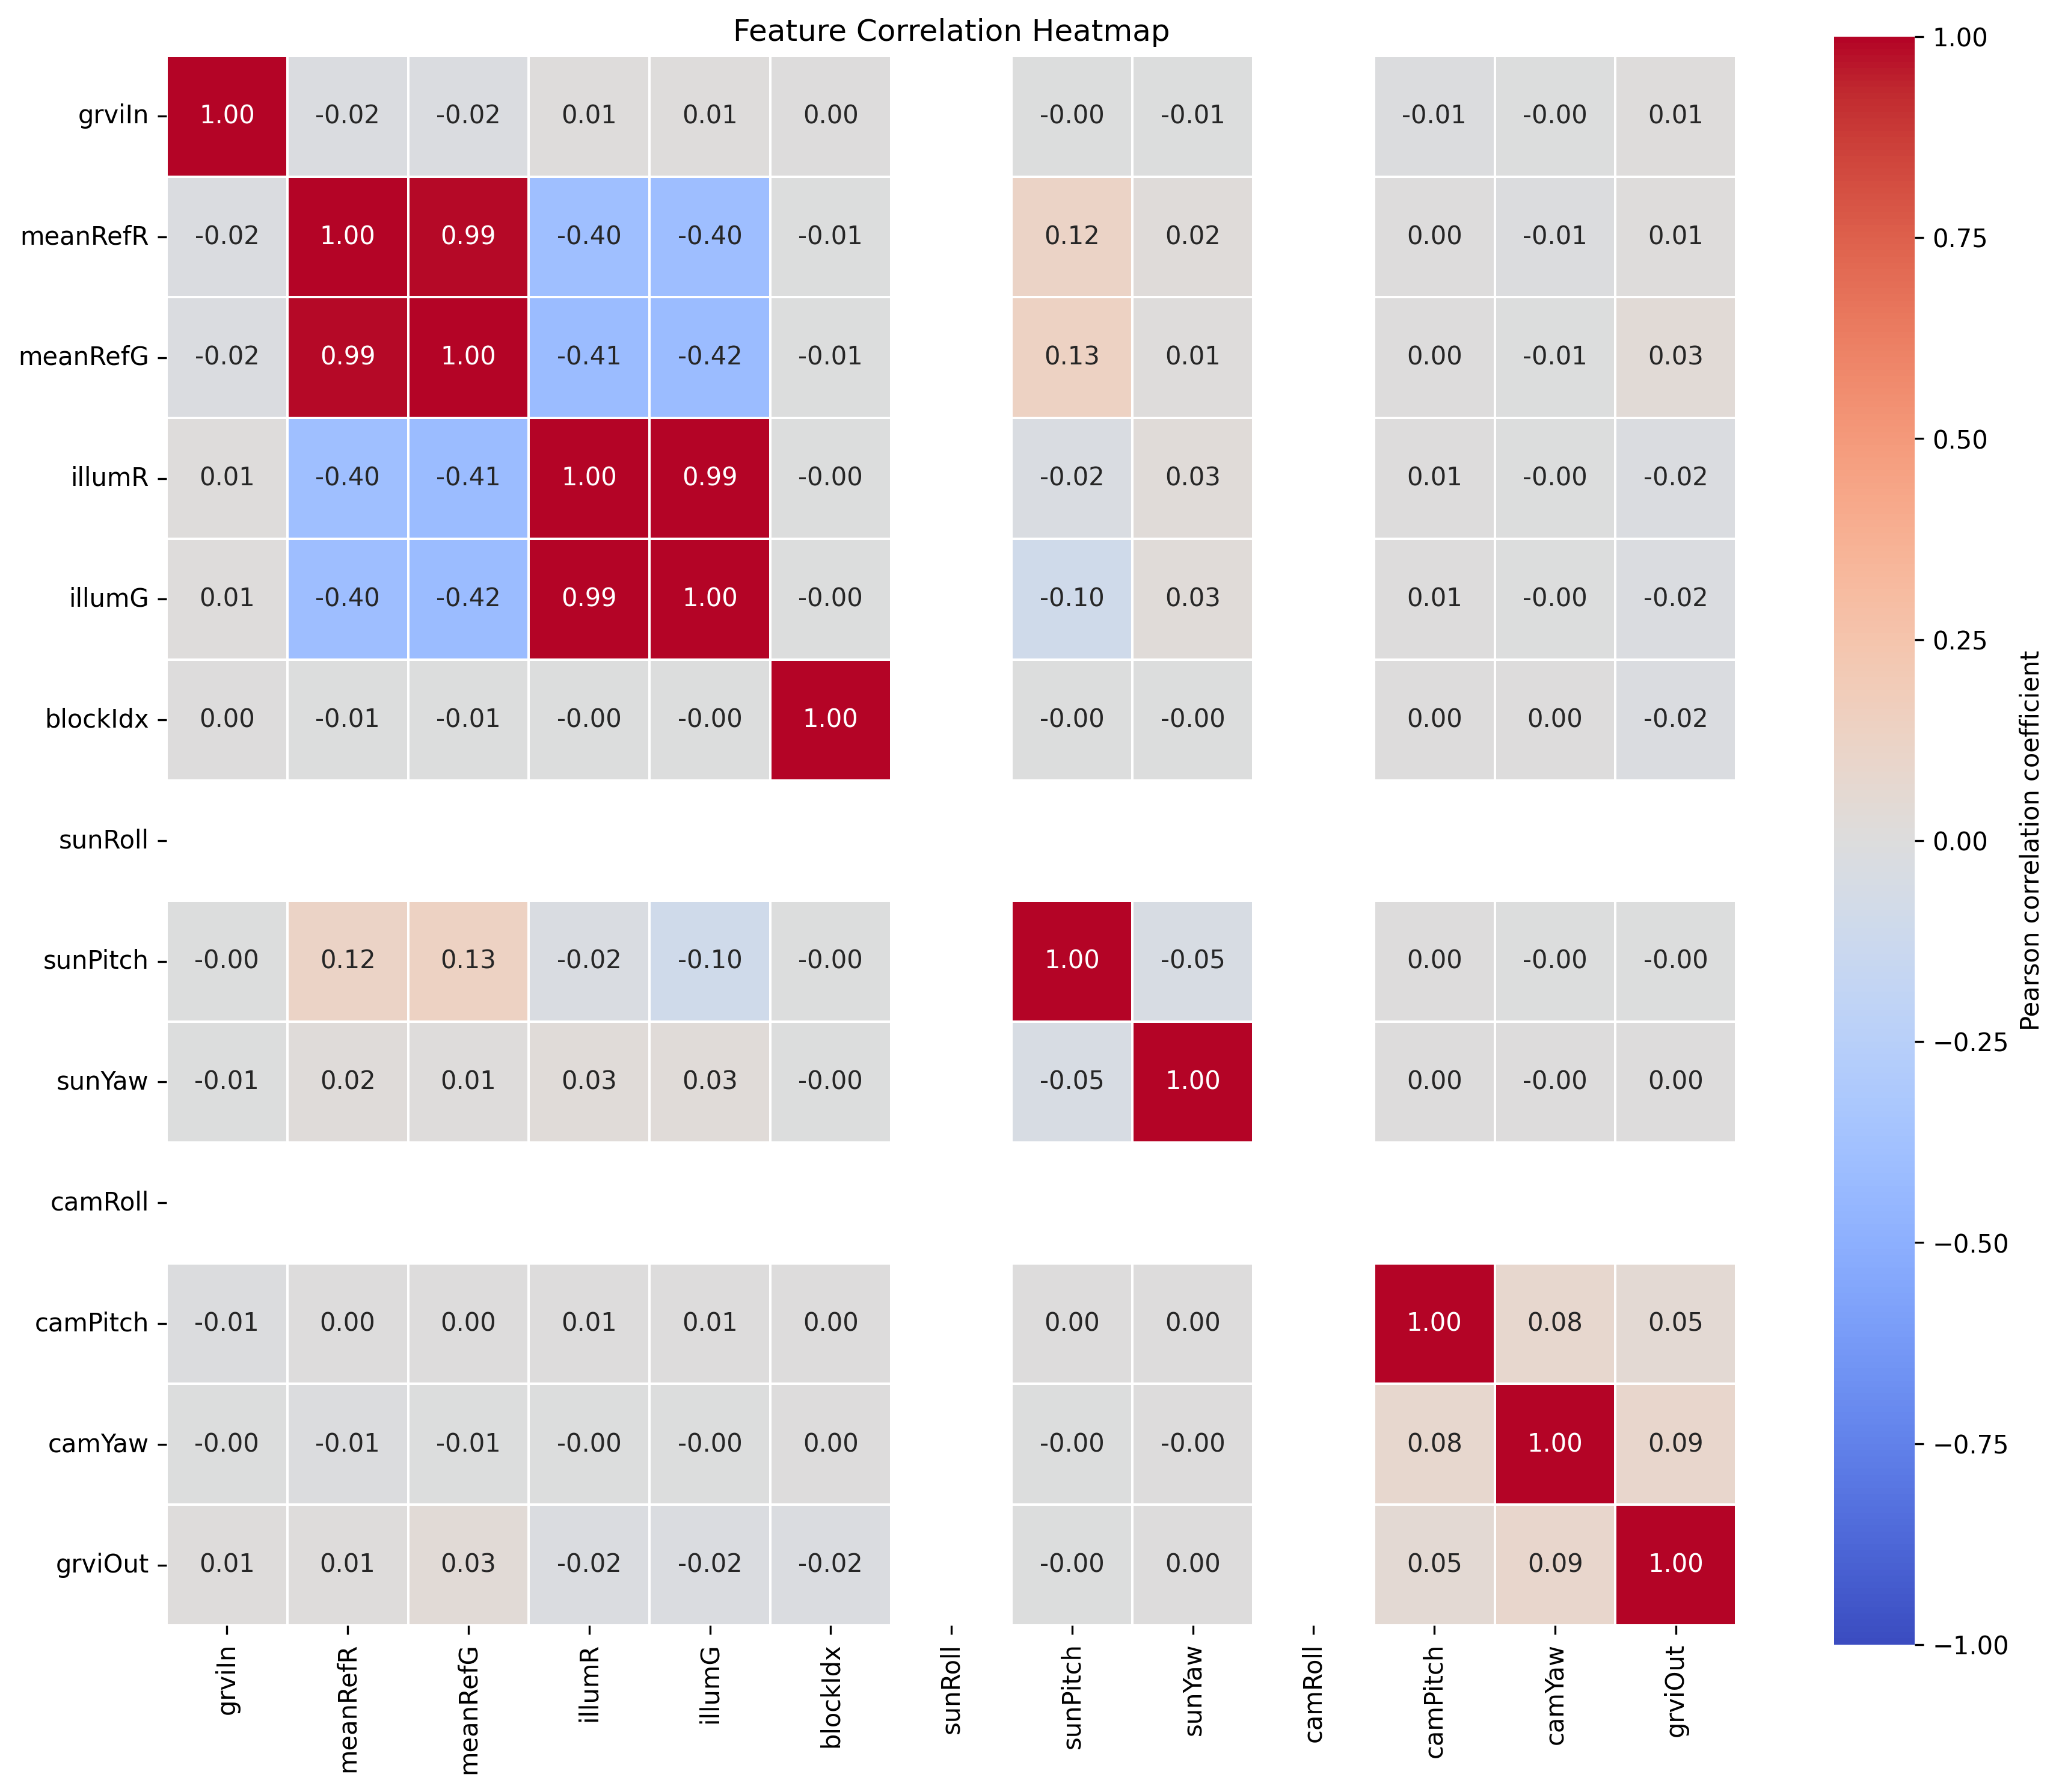
\includegraphics[width=1\linewidth]{images/correlation_trees-dl-aoi.png}
    \caption{Correlation heatmap presenting the Pearson Correlation Coefficient calculated between all the features of the dataset.}
    \label{correlation-hm}
\end{figure}


Another way to identify which features could be safely dropped without major loss in predictive performance is by determining the importance of each feature. All of the frameworks used for their implementations of classical ML models provide tools for calculating feature importance, such as permutation feature importance, impurity-based importance, etc. Since these methods are model-dependent, they are discussed later on, after the models' implementations, in Section~\ref{pract-feature-eng}.

\subsubsection{Principal Component Analysis (PCA)}

Principal component analysis (PCA) aims to reduce the complexity of a given dataset by replacing its features with new, uncorrelated ones, named principal components, while attempting to retain as much useful information as possible. Mathematically, this means that the original data are projected to a lower dimensional subspace, in a way that variance of the projected data is maximized (as much as possible of the original variance is preserved) \cite{shlens2005pca}.

I experimented with PCA, aiming to determine weather it achieves dimensionality reduction more efficiently than the rest of the methods tested throughout this study. This included testing different amounts of principal components, seeking for a sweet-spot between low count of principal components and high predictive accuracy. The results are discussed in !!!!!!!!!.

\subsubsection{Substituting Sun's and SCC's Roll, Pitch and Yaw with a Single Number}

Among the attributes that were originally planned to be included in the datasets, there were a total of six regarding the sun-SCC geometry: the sun's and SCC's roll, pitch and yaw (RPY). Although some of them could be easily removed during the feature selection, it is possible to reduce all of them to a single feature, by replacing them with the relative azimuth angle between the sun and the SCC. 

To reduce the six RPY features, the first step was to convert these values into the corresponding rotation matrices of the two actors' unit vectors. For a given set of RPY angles, the rotation matrix is defined as \cite{rot-mat}:

\[ 
R = R_z(\mathrm{yaw})R_y(\mathrm{pitch})R_x(\mathrm{roll}),
\]


where

\[
R_z(\mathrm{yaw}) =
\begin{bmatrix}
\cos(\mathrm{yaw}) & -\sin(\mathrm{yaw}) & 0\\
\sin(\mathrm{yaw}) & \cos(\mathrm{yaw}) & 0\\
0 & 0 & 1
\end{bmatrix},
\]

\[
R_y(\mathrm{pitch}) =
\begin{bmatrix}
\cos(\mathrm{pitch}) & 0 & \sin(\mathrm{pitch})\\
0 & 1 & 0\\
-\sin(\mathrm{pitch}) & 0 & \cos(\mathrm{pitch})
\end{bmatrix},
\]

and

\[
R_x(\mathrm{roll}) =
\begin{bmatrix}
1 & 0 & 0\\
0 & \cos(\mathrm{roll}) & -\sin(\mathrm{roll})\\
0 & \sin(\mathrm{roll}) & \cos(\mathrm{roll})
\end{bmatrix}.
\]

Thus, separate rotation matrices \(R_c\) and \(R_s\) were calculated for the SCC and the Sun, respectively.

In Unreal Engine (UE), the \(x\)-axis represents the forward direction, while the \(y\)-axis represents the right direction. Therefore, the SCC's local forward and right directions can initially be represented by the unit vectors:

\[
\begin{bmatrix}1\\0\\0\end{bmatrix}
\quad\text{and}\quad
\begin{bmatrix}0\\1\\0\end{bmatrix}.
\]

These vectors were rotated using \(R_c\) so that they followed the actual orientation of the SCC. The resulting forward and right vectors were therefore calculated as:

\[
f_c = R_c
\begin{bmatrix}
1\\0\\0
\end{bmatrix},
\qquad
r_c = R_c
\begin{bmatrix}
0\\1\\0
\end{bmatrix}.
\]

Together, \(f_c\) and \(r_c\) define the SCC-relative plane onto which the sun's direction can be projected. 


For the sun, on the other hand, only the forward direction is required since its only used to determine the direction in which it is pointing. Its corresponding vector was obtained as:

\[
s = R_s
\begin{bmatrix}
1\\0\\0
\end{bmatrix}.
\]

In general, the angle between two arbitrary vectors \(a\) and \(b\) can be determined through their dot product, using \cite{wikipedia2025dot}:

\[
\theta =
\arccos\left(
\frac{a\cdot b}
{\lVert a\rVert\lVert b\rVert}
\right).
\]

In this case, \(f_c\), \(r_c\), and \(s\) are unit vectors and therefore have a magnitude of one. Consequently, the expression simplifies to:

\[
\theta = \arccos(a\cdot b).
\]

The dot product between the sun direction and the SCC forward direction consequently represents the cosine component of the relative angle,

\[
\frac{s\cdot f_c}
{\lVert s\rVert\lVert f_c\rVert}
=
\cos(\theta)
\quad\Rightarrow\quad
s\cdot f_c = \cos(\theta),
\]

while, since the SCC's right direction is perpendicular to its forward direction, the corresponding right component is:

\[
s\cdot r_c = \sin(\theta).
\]

These two components can then be combined using the two-argument arctangent function. In general \cite{wikipedia2025atan2}:

\[
\theta = \operatorname{atan2}(y,x),
\]

where

\[
x=r\cos(\theta),
\qquad
y=r\sin(\theta).
\]

Therefore, using the forward component as \(x\) and the right component as \(y\), the relative sun–SCC azimuth is obtained as

\begin{equation}
    \theta =
    \operatorname{atan2}
    \left(
    s\cdot r_c,\,
    s\cdot f_c
    \right)
\end{equation}


I later coded this sequence of operations into a Python script that, given a dataset including the sun's and SCC's RPY as input features, replaces the six rotation columns with a single relative azimuth angle column. The predictive and computational performance impacts of this change are discussed in !!!!!!!!!.

\subsection{Standard Scaling}
\label{standscale}

As demonstrated in Section~\ref{diffuse-aff-grvi}, the perceived GRVI values calculated using luminance and illuminance information under diffuse lighting conditions tend to be concentrated within a particularly narrow range, even after removing the removal of soil. While this characteristic is not inherently problematic, differences in the numerical scales of input features can disproportionately influence certain scale-sensitive ML algorithms, regardless of the features' actual predictive importance \cite{google_normalization}. In our case, while the average perceived GRVI values are within the range $\begin{bmatrix}0.059267, 0.184111\end{bmatrix}$, the illuminance values range between $0.253$ and $1467.124$. Tree-based methods, which were the primary architecture I experimented with in this work, are insensitive to feature scaling \cite{sklearn_feature_scaling}. However, other algorithms, particularly those relying on distance calculations, regularization, or gradient-based optimization, such as Ridge Regression, Lasso Regression, Support Vector Regression and Neural Networks, can be significantly affected by such differences.

A solution to the problems introduced by having features on different scales is bringing all features to a common scale. This eliminates disproportionate influence on the ouput, caused solely by a feature's magnitude. In this study, I used Scikit-learn's implementation of Z-score scaling, called Standard Scaling, to scale the data. Z-score scaling transforms each numerical feature so that it has mean equal to $0$ and standard deviation equal to $1$. As expected, the application of Standard Scaling to the datasets did not affect tree-based models, the impact on the rest of the models though was noticeable. Figure~\ref{ss-before-after} illustrates the feature values corresponding to the areas of interest of frames captured during one of the render sequences, before and after Standard Scaling.

\begin{figure}[htb]
    \centering
    
    \begin{subfigure}{0.48\linewidth}
        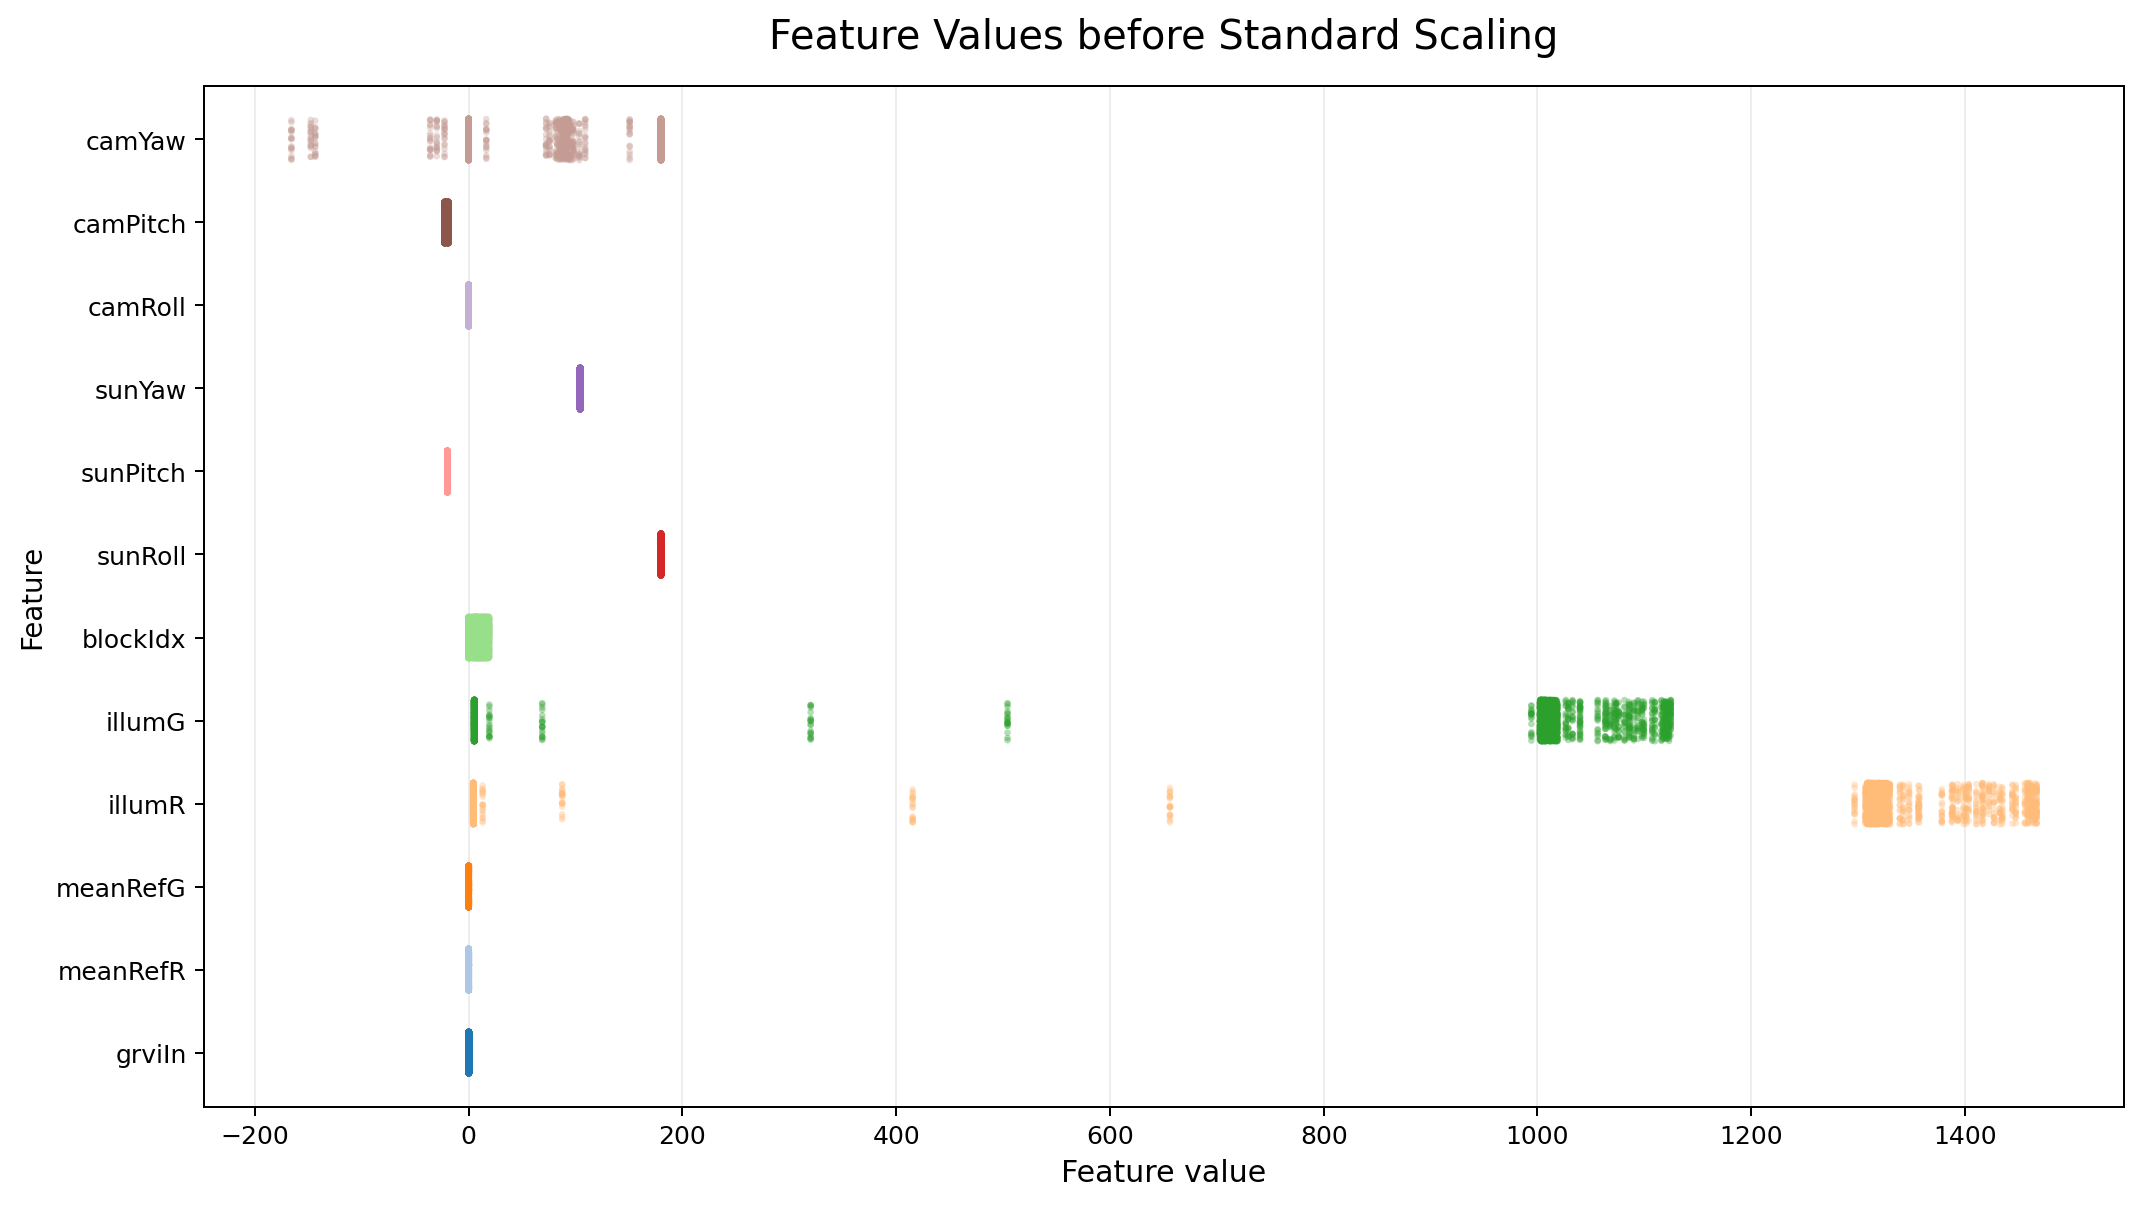
\includegraphics[width=\linewidth]{images/before_standard_scaling.png}
        \caption{Feature values before Standard Scaling}
        \label{ss-before}
    \end{subfigure}\hfill
    \begin{subfigure}{0.48\linewidth}
        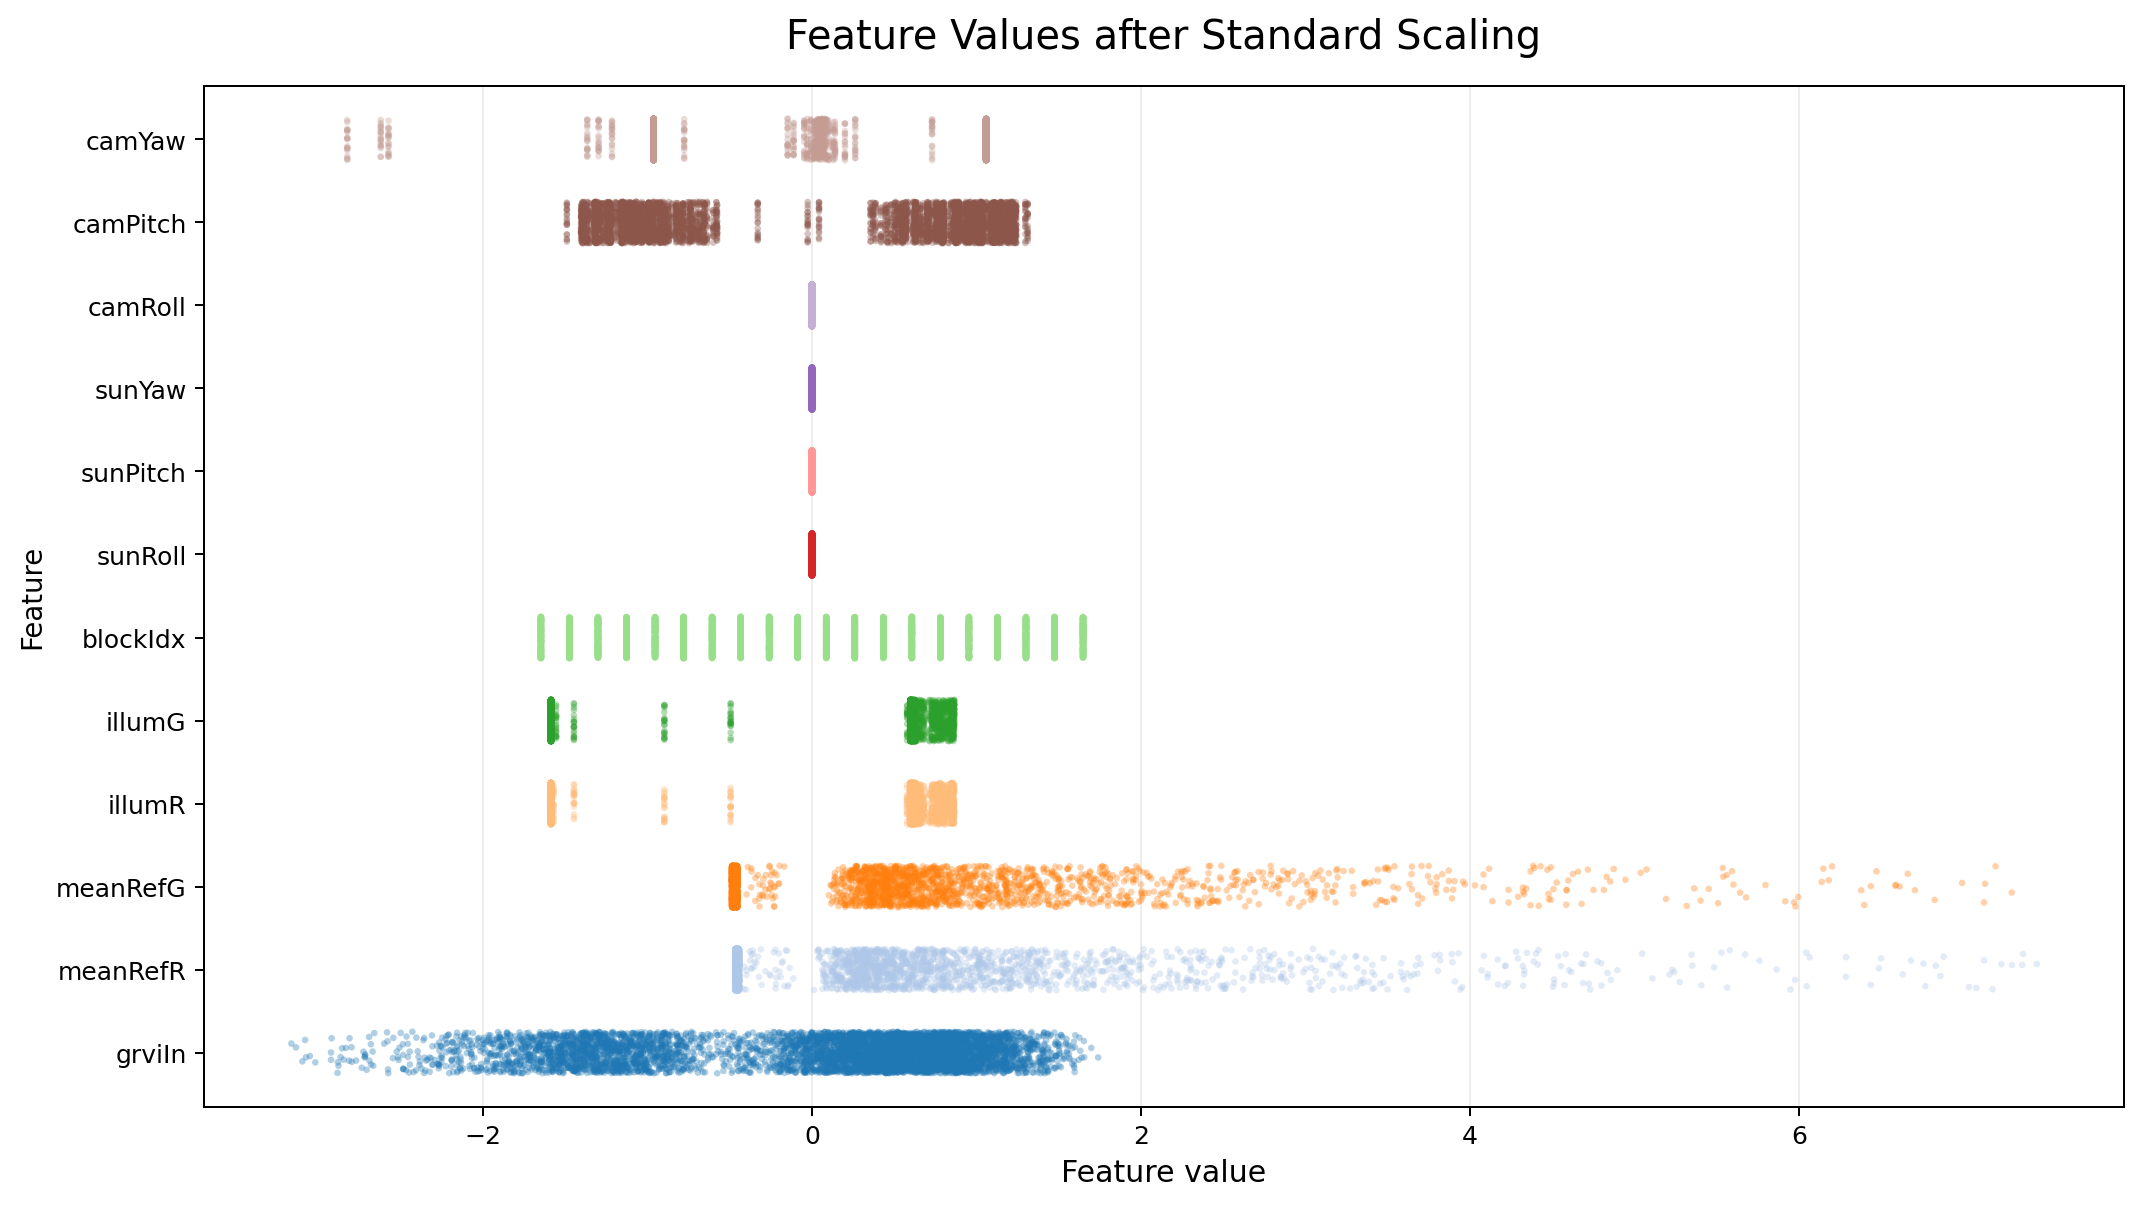
\includegraphics[width=\linewidth]{images/after_standard_scaling.png}
        \caption{Feature values after Standard Scaling}
        \label{ss-after}
    \end{subfigure}
    
    \caption{Scatter plots of the feature values, acquired after a single render sequence. Plot~\ref{ss-before} presents the original feature values, while Plot~\ref{ss-after} shows their standardized counterparts.}
    \label{ss-before-after}
\end{figure}
    \chapter{Machine Learning Models Development}
\label{chap7}

With enough instances of the examined phenomena captured and organized in datasets, the final step of this work was to develop a machine learning model that, given the selected set of features as an input, would be able to output the ground truth GRVI value of an examined area. Essentially, the objective was to examine whether an ML solution could address the different sources of error, without us needing to identify and model them mathematically.

During this process, I tested various algorithms, most of which belong in the same model family. Comparing them in terms of accuracy and efficiency lead to a single model proposed for embedded deployment. A total of five different model types were testd. Four of them belong to the tree-based ensemble learning methods family, one is a Multilayer Perceptron (MLP) and one is a mixture of experts, that combines multiple architectures.


    %\include{chapter...} % προσθέστε όσα χρειάζεται
    \chapter{Συμπεράσματα}
\label{chap_last}

Εδώ εξηγούμε ότι θα συνοψίσουμε την μελέτη που εκπονήθηκε στα πλαίσια της διπλωματικής.

\section{Σύνοψη και συμπεράσματα}

Εδώ συνοψίζουμε τα αποτελέσματα της διπλωματικής και περιγράφουμε τα συμπεράσματα που προέκυψαν, αρνητικά και θετικά. Επιβεβαιώνουμε την συνεισφορά της διπλωματικής στα προβλήματα που αναφέραμε στην εισαγωγή.

\section{Μελλοντικές επεκτάσεις}

Εδώ δίνουμε ιδέες για επέκταση της διπλωματικής.

%
%%%%%%%%%%%%%%%%%%%%%%%%%%%%%%%%%%%%%%%%%%%%%%%%%%%%


%\backmatter % μην ενεργοποιείτε την εντολή
% Βιβλιογραφία - Αναφορές
	\bibliography{references}


%%%%%%%%%%%%%%%%%%%%%%%%%%%%%%%%%%%%%%%%%%%%%%%%%%%%%
%% APPENDICES (optional) / ΠΑΡΑΡΤΗΜΑΤΑ (ΠΡΟΑΙΡΕΤΙΚΑ)
%%

% Εάν υπάρχουν περισσότερα από ένα Παραρτήματα
% είναι ενεργή η ακόλουθη εντολή
% και ανενεργή για μεμονωμένο Παράρτημα
    % Να μην τροποποποιηθεί

\cleardoublepage\thispagestyle{plain}
~\vfill
\ifgrthesisoption
    \centerline{\huge\bf ΠΑΡΑΡΤΗΜΑΤΑ}\phantomsection
    \addcontentsline{toc}{chapter}{ΠΑΡΑΡΤΗΜΑΤΑ}
\else
    \centerline{\huge\bf APPENDICES}\phantomsection
    \addcontentsline{toc}{chapter}{APPENDICES}
\fi
\vfill

% Μην τροποποιήσετε τις ακόλουθες εντολές
\ifgrthesisoption
    \renewcommand{\chaptername}{Παράρτημα}
\else
    \renewcommand{\chaptername}{Appendix}
\fi

% Πριν το κάθε Παράρτημα (για περισσότερα από ένα), 
% ρυθμίζεται η κατάλληλη αλφαβητική αρίθμηση
    \renewcommand{\thechapter}{A} 
  	% Παράρτημα A

\chapter{Τίτλος Παραρτήματος \label{appendixA}}



Τα παραρτήματα περιλαμβάνουν συνοδευτικό, υποστηρικτικό υλικό (πίνακες, φωτογραφίες, ερωτηματολόγια, στατιστικά στοιχεία, αποδείξεις, περιγραφές  λογισμικών  προγραμμάτων,  παραδείγματα,  περιγραφές 
πολύπλοκων διαδικασιών, λίστα με πρωτογενή στοιχεία, λεπτομερής περιγραφή και προδιαγραφές εξοπλισμού, οδηγίες εγκατάστασης λογισμικού, κ.λπ.), ή αλλιώς ό,τι θεωρείται χρήσιμο να περιγραφεί, αλλά δεν συνηθίζεται να 
εντάσσεται μέσα στο κυρίως κείμενο της Εργασίας.  Στο κυρίως κείμενο της Εργασίας πρέπει να γίνονται οι κατάλληλες παραπομπές προς τα παραρτήματα, όπου το κείμενο σχετίζεται με υλικό που περιλαμβάνεται σε αυτά. Ένα παράρτημα, αναλόγως με το περιεχόμενό του, μπορεί να είναι ενιαίο, ή να χωρίζεται σε ενότητες.


\section{Δυνατότητες του \LaTeX}

Kαθώς το παρόν αποτελεί ένα πρότυπο συγγραφής διπλωματικών εργασιών, στην ενότητα αυτή επιδεικνύονται ορισμένες από τις δυνατότητες το \LaTeX οι οποίες μπορούν να αξιοποιηθούν στο κείμενο μιας διπλωματικής εργασίας (μια καλή πηγή για τη διερεύνηση των δυνατοτήτων του \LaTeX είναι η ιστοσελίδα {\small\url{https://www.overleaf.com/learn/latex/Main_Page}}).

\subsection{Πίνακες}
Ο Πίνακας~\ref{tab1} είναι ένα παράδειγμα πίνακα σχεδιασμένου με εντολές του περιβάλλοντος \texttt{tabular}.
\begin{table}[htb]
\centering
\caption{Παράμετροι πειραμάτων}
\label{tab1}
\begin{tabular}{|c|>{\centering\arraybackslash}m{8cm}|}
\hline Πλήθος κελιών καννάβου \textit{{c}} $\times$ \textit{{c}} & 50 $\times$ 50, 100 $\times$ 100, 200 $\times$ 200, \textbf{250} $\times$ \textbf{250}, 500 $\times$ 500, 1000 $\times$ 1000  \\
\hline Τυπική απόκλιση $\sigma$ & 25{m}, 50{m}, 75{m}, \textbf{100{m}}, 150{m}, 200{m} \\
\hline Αριθμός εγγύτερων γειτόνων \textit{{k}} & 1, 2, \textbf{3}, 4, 5, 10, 20 \\
\hline Πιθανοτικό κατώφλι $\theta$ & 50$\%$, 60$\%$, 70$\%$, \textbf{75$\%$}, 80$\%$, 90$\%$, 99$\%$ \\
\hline  
\end{tabular}

\end{table} 

\subsection{Διαγράμματα - Γραφικές παραστάσεις}
Στο Σχήμα~\ref{fig1}, παρουσιάζεται ένα παράδειγμα γραφικής παράστασης σχεδιασμένης με το Gnuplot. Ένας άλλος τρόπος κατασκευής τέτοιων παραστάσεων/διαγραμμάτων είναι με χρήση του πακέτου pgfplots (\url{http://pgfplots.sourceforge.net/}).
\begin{figure}[htb]
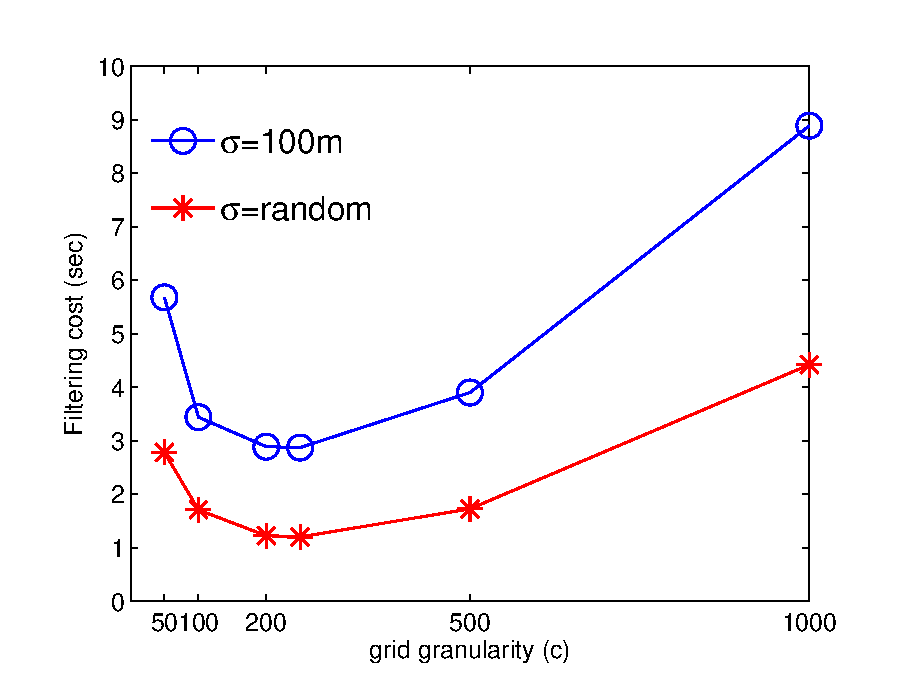
\includegraphics[scale=0.7]{figures/grid_granularity.eps}
\centering
\caption{Κλιμάκωση χρόνου εκτέλεσης για διάφορες υποδιαιρέσεις του καννάβου}	
\label{fig123}
\end{figure} 

Στο Σχήμα~\ref{Quadtree}, παρουσιάζεται ένα παράδειγμα εισαγωγής σχήματος/εικόνας που περιέχεται σε αρχείο pdf, ενώ στο Κεφάλαιο \ref{chap2}, στο Σχήμα \ref{dataconnection} παρουσιάζεται ένα παράδειγμα εισαγωγής σχήματος/εικόνας που περιέχεται σε αρχείο jpg.
\begin{figure}[htb]
\centering
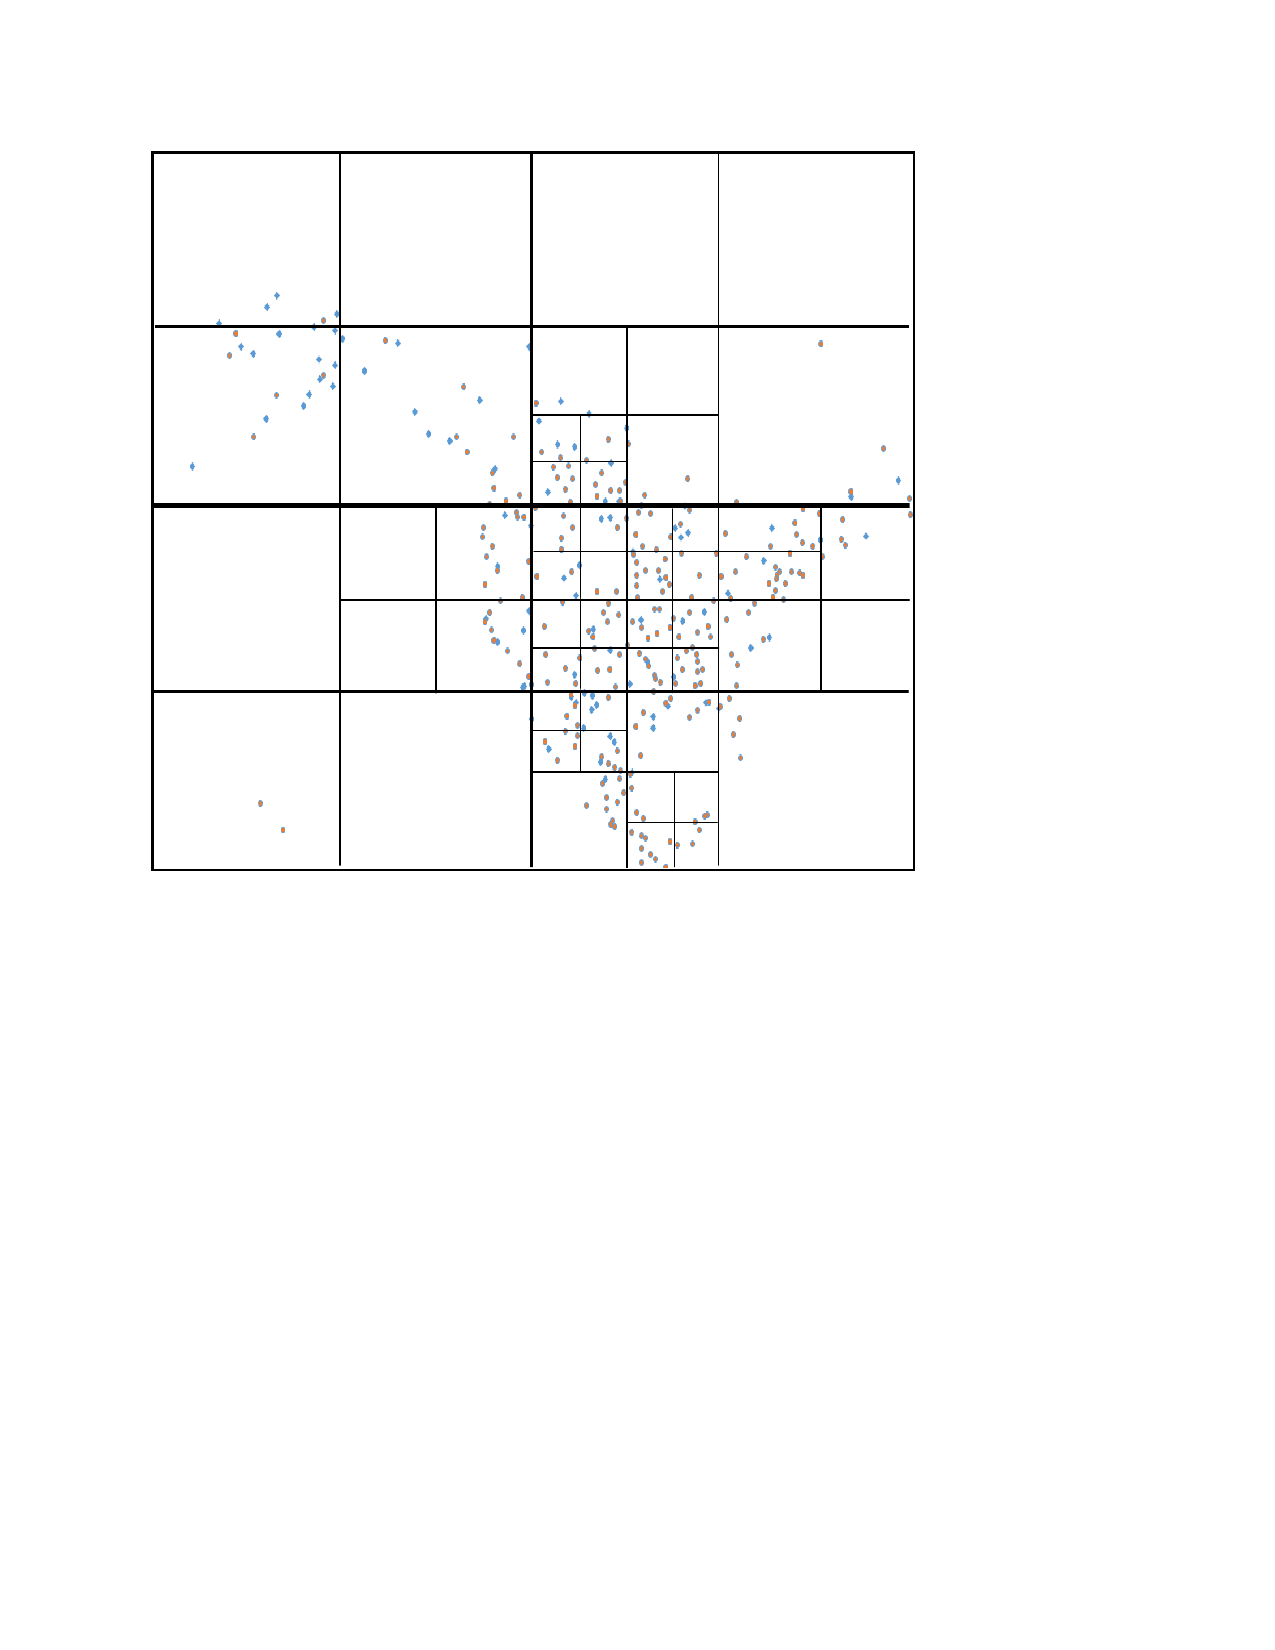
\includegraphics[width = 0.57\columnwidth, height = 8.5cm ]{figures/quadtree.pdf}
\caption{Quadtree partitioning.}
\label{Quadtree}
\end{figure}

\subsection{Σχήματα}
Ακολουθεί στο Σχήμα~\ref{fig2} ένα παράδειγμα σχήματος φτιαγμένου με εντολές του πακέτου Ti\textit{k}Z.
\begin{figure}[htb]
\begin{center}
\begin{tikzpicture}
\draw (-2,0) -- (2,0);
\filldraw [gray] (0,0) circle (2pt);
\draw (-2,-2) .. controls (0,0) .. (2,-2);
%\draw (-2,2) .. controls (-1,0) and (1,0) .. (2,2);
 \draw[gray, thick] (-1,2) -- (2,-4);
\draw[gray, thick] (-1,-1) -- (2,2);
\filldraw[black] (0,0) circle (2pt)  ;
\end{tikzpicture}
\end{center}
\caption{Παράδειγμα σχήματος με εντολές του πακέτου Ti\textit{k}Z}	
\label{fig12223}
\end{figure}

\subsection{Μαθηματικές εκφράσεις}
Ακολουθούν παραδείγματα μαθηματικών εκφράσεων.
\begin{eqnarray}
\hat{I}(x,u,t)     &=& dist(y(t_f),\Gamma)
+  \int_t^{t_f} \: {\cal L}( y(s),u(s),s) \: ds
\label{con11b}
\end{eqnarray}

     \[
        \frac{d}{dx}\left( \int_{0}^{z} f(u)\,du\right)=f(x).
     \]

\subsection{Αλγόριθμοι}
Ακολουθεί ο Αλγόριθμος~\ref{alg1}, ο οποίος είναι μορφοποιημένος με τα πακέτα algorithm και algorithmic.

\begin{algorithm}[htb]
\caption{\ \ \ Probabilistic $k\theta NN$ Monitoring}
\begin{algorithmic}[1]
\begin{small}

\STATE{\bf Procedure} {\em VerifyCandidate} (focal query point $q$, threshold $\theta$, object $o$, list of auxiliary objects $P$, distance $kMAXDIST$) 

\IF { $\Phi(o, kMAXDIST) \geq \theta$ {\bf and} $L_2(q, o) \leq L_2(q, P.$top()) }

\STATE {$P$.pop()};   \ \ \ \ \ \ \ \ {\em //Replace the most extreme element in $P$, since candidate $o$ ... }

\STATE {$P$.push($o$)};  \ \ \ \ \ {\em //... has enough probability and has its mean closer to focal $q$ }

\ENDIF

\STATE {\bf End Procedure}


\end{small}
\end{algorithmic}
\label{alg1}
\end{algorithm}

\subsection{Θεωρήματα, Πορίσματα, Ορισμοί, κλπ.}

Ακολουθεί παράδειγμα θεωρήματος από την ιστοσελίδα  {\small\url{https://www.overleaf.com/learn/latex/Theorems_and_proofs}}

\begin{theorem}
Let $f$ be a function whose derivative exists in every point, then $f$ 
is a continuous function.
\end{theorem}

\subsection{Απαριθμήσεις}

Μια απαρίθμηση (itemized list) βοηθά στην παρουσίαση μιας σειράς περιπτώσεων με σαφήνεια.
Ακολουθεί παράδειγμα.

H εκπαίδευση στην Ελλάδα διακρίνεται σε:
\begin{itemize}
\item Πρωτοβάθμια 
\item Δευτεροβάθμια 
\item Τριτοβάθμια 
\end{itemize}

\subsection{Είδη πηγών στις αναφορές}

Στο references.bib μπορεί να δει κανείς πώς γράφονται διάφορα είδη πηγών 
(Βιβλία Ξενόγλωσσα \cite{goossens93},
Βιβλία Ελληνικά \cite{greekbook},
Άρθρα σε επιστημονικά περιοδικά \cite{LiArTs13},
Άρθρα σε επιστημονικά συνέδρια \cite{dcis2011},
Ιστοσελίδες \cite{LaTeXProject},
Πτυχιακές Εργασίες \cite{elli05},
Διπλωματικές Εργασίες \cite{zoi04},
Μεταπτυχιακές Διπλωματικές Εργασίες \cite{master04},
Διδακτορικές Διατριβές \cite{phd045},
Τεχνικές Αναφορές \cite{MSU-CSE-05-29},
Διπλώματα Ευρεσιτεχνίας \cite{viswanathan2014convenient}),
Κεφάλαια σε συλλογικούς τόμους
\cite{[PS11]}.

	
% %	
    \renewcommand{\thechapter}{B}
    % Παράρτημα B

 
\chapter{Τίτλος 2ου Παραρτήματος\label{appendixB}}

Τα παραρτήματα περιλαμβάνουν συνοδευτικό, υποστηρικτικό υλικό (πίνακες, φωτογραφίες, ερωτηματολόγια, στατιστικά στοιχεία, αποδείξεις, περιγραφές  λογισμικών  προγραμμάτων,  παραδείγματα,  περιγραφές 
πολύπλοκων διαδικασιών, λίστα με πρωτογενή στοιχεία, λεπτομερής περιγραφή και προδιαγραφές εξοπλισμού, οδηγίες εγκατάστασης λογισμικού, κ.λπ.), ή αλλιώς ό,τι θεωρείται χρήσιμο να περιγραφεί, αλλά δεν συνηθίζεται να 
εντάσσεται μέσα στο κυρίως κείμενο της Εργασίας.  Στο κυρίως κείμενο της Εργασίας πρέπει να γίνονται οι κατάλληλες παραπομπές προς τα παραρτήματα, όπου το κείμενο σχετίζεται με υλικό που περιλαμβάνεται σε αυτά. Ένα παράρτημα, αναλόγως με το περιεχόμενό του, μπορεί να είναι ενιαίο, ή να χωρίζεται σε ενότητες.

% Εάν υπάρχει μόνο ένα Παράρτημα,
% μπαίνουν σε σχόλια οι παραπάνω γραμμές 
% και ρυθμίζεται αρίθμηση χωρίς γράμμα
%   \renewcommand{\thechapter}{} 
%   \renewcommand{\thesection}{\arabic{section}}
%
% Ακολουθεί αρχείο μεμονωμένου Παραρτήματος
% (διαφορετική δομή από appA/appΒ)
%   % Μεμονωμένο Παράρτημα 
% ορίζεται ο τίτλος του παραρτήματος
\edef\chaptertitle{Τίτλος Παραρτήματος}
\label{appendix}

% Μην τροποποιήσετε τις ακόλουθες εντολές
\chapter*{\chaptername\\\vspace{1cm} \chaptertitle} 
\addcontentsline{toc}{chapter}{\chaptername\texorpdfstring{\\}~\chaptertitle}
\setcounter{section}{0}
\renewcommand{\chaptermark}[1]{\markboth{\textit{\chaptername. \chaptertitle}}{}}
\chaptermark{}


Τα παραρτήματα περιλαμβάνουν συνοδευτικό, υποστηρικτικό υλικό (πίνακες, φωτογραφίες, ερωτηματολόγια, στατιστικά στοιχεία, αποδείξεις, περιγραφές  λογισμικών  προγραμμάτων,  παραδείγματα,  περιγραφές 
πολύπλοκων διαδικασιών, λίστα με πρωτογενή στοιχεία, λεπτομερής περιγραφή και προδιαγραφές εξοπλισμού, οδηγίες εγκατάστασης λογισμικού, κ.λπ.), ή αλλιώς ό,τι θεωρείται χρήσιμο να περιγραφεί, αλλά δεν συνηθίζεται να 
εντάσσεται μέσα στο κυρίως κείμενο της Εργασίας.  Στο κυρίως κείμενο της Εργασίας πρέπει να γίνονται οι κατάλληλες παραπομπές προς τα παραρτήματα, όπου το κείμενο σχετίζεται με υλικό που περιλαμβάνεται σε αυτά. Ένα παράρτημα, αναλόγως με το περιεχόμενό του, μπορεί να είναι ενιαίο, ή να χωρίζεται σε ενότητες.


\section{Δυνατότητες του \LaTeX}

Kαθώς το παρόν αποτελεί ένα πρότυπο συγγραφής διπλωματικών εργασιών, στην ενότητα αυτή επιδεικνύονται ορισμένες από τις δυνατότητες το \LaTeX οι οποίες μπορούν να αξιοποιηθούν στο κείμενο μιας διπλωματικής εργασίας (μια καλή πηγή για τη διερεύνηση των δυνατοτήτων του \LaTeX είναι η ιστοσελίδα {\small\url{https://www.overleaf.com/learn/latex/Main_Page}}).

\subsection{Πίνακες}
Ο Πίνακας~\ref{tab1} είναι ένα παράδειγμα πίνακα σχεδιασμένου με εντολές του περιβάλλοντος \texttt{tabular}.
\begin{table}[htb]
\centering
\caption{Παράμετροι πειραμάτων}
\label{tab1}
\begin{tabular}{|c|>{\centering\arraybackslash}m{8cm}|}
\hline Πλήθος κελιών καννάβου \textit{{c}} $\times$ \textit{{c}} & 50 $\times$ 50, 100 $\times$ 100, 200 $\times$ 200, \textbf{250} $\times$ \textbf{250}, 500 $\times$ 500, 1000 $\times$ 1000  \\
\hline Τυπική απόκλιση $\sigma$ & 25{m}, 50{m}, 75{m}, \textbf{100{m}}, 150{m}, 200{m} \\
\hline Αριθμός εγγύτερων γειτόνων \textit{{k}} & 1, 2, \textbf{3}, 4, 5, 10, 20 \\
\hline Πιθανοτικό κατώφλι $\theta$ & 50$\%$, 60$\%$, 70$\%$, \textbf{75$\%$}, 80$\%$, 90$\%$, 99$\%$ \\
\hline  
\end{tabular}

\end{table}

\subsection{Διαγράμματα - Γραφικές παραστάσεις}
Στο Σχήμα~\ref{fig1}, παρουσιάζεται ένα παράδειγμα γραφικής παράστασης σχεδιασμένης με το Gnuplot.
\begin{figure}[htb]
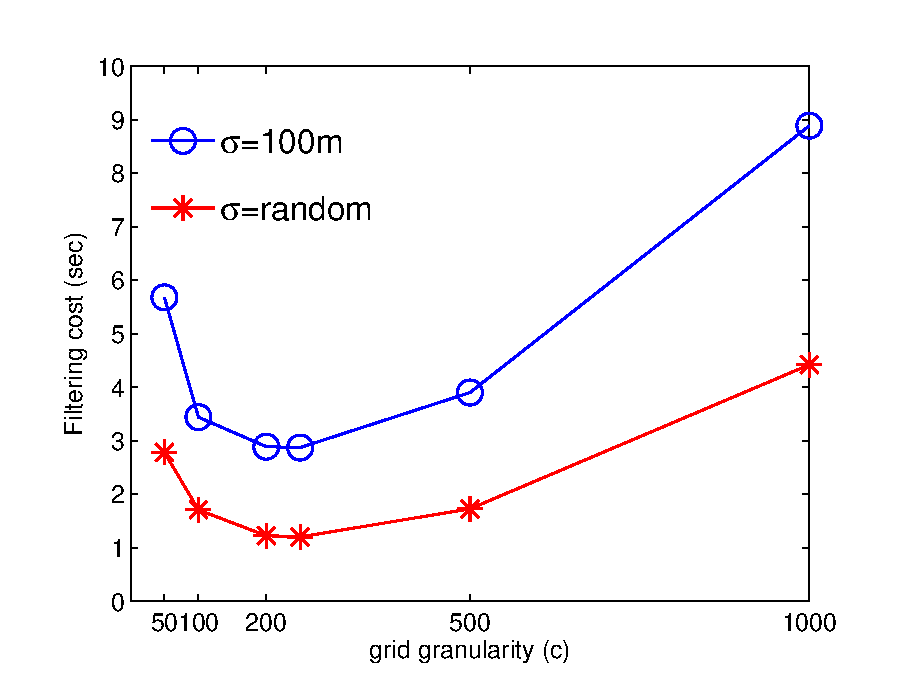
\includegraphics[scale=0.7]{figures/grid_granularity.eps}
\centering
\caption{Κλιμάκωση χρόνου εκτέλεσης για διάφορες υποδιαιρέσεις του καννάβου}	
\label{fig1}
\end{figure} 

\subsection{Σχήματα}
Ακολουθεί στο Σχήμα~\ref{fig2} ένα παράδειγμα σχήματος φτιαγμένου με εντολές του πακέτου Ti\textit{k}Z.
\begin{figure}[htb]
\begin{center}
\begin{tikzpicture}
\draw (-2,0) -- (2,0);
\filldraw [gray] (0,0) circle (2pt);
\draw (-2,-2) .. controls (0,0) .. (2,-2);
%\draw (-2,2) .. controls (-1,0) and (1,0) .. (2,2);
 \draw[gray, thick] (-1,2) -- (2,-4);
\draw[gray, thick] (-1,-1) -- (2,2);
\filldraw[black] (0,0) circle (2pt)  ;
\end{tikzpicture}
\end{center}
\caption{Παράδειγμα σχήματος με εντολές του πακέτου Ti\textit{k}Z}	
\label{fig2}
\end{figure}

\subsection{Αλγόριθμοι}
Ακολουθεί ο Αλγόριθμος~\ref{alg1}, ο οποίος είναι μορφοποιημένος με τα πακέτα algorithm και algorithmic.

\begin{algorithm}[htb]
\caption{\ \ \ Probabilistic $k\theta NN$ Monitoring}
\begin{algorithmic}[1]
\begin{small}

\STATE{\bf Procedure} {\em VerifyCandidate} (focal query point $q$, threshold $\theta$, object $o$, list of auxiliary objects $P$, distance $kMAXDIST$) 

\IF { $\Phi(o, kMAXDIST) \geq \theta$ {\bf and} $L_2(q, o) \leq L_2(q, P.$top()) }

\STATE {$P$.pop()};   \ \ \ \ \ \ \ \ {\em //Replace the most extreme element in $P$, since candidate $o$ ... }

\STATE {$P$.push($o$)};  \ \ \ \ \ {\em //... has enough probability and has its mean closer to focal $q$ }

\ENDIF

\STATE {\bf End Procedure}


\end{small}
\end{algorithmic}
\label{alg1}
\end{algorithm}

\subsection{Μαθηματικές εκφράσεις}
Ακολουθούν παραδείγματα μαθηματικών εκφράσεων.
\begin{eqnarray}
\hat{I}(x,u,t)     &=& dist(y(t_f),\Gamma)
+  \int_t^{t_f} \: {\cal L}( y(s),u(s),s) \: ds
\label{con11b}
\end{eqnarray}

     \[
        \frac{d}{dx}\left( \int_{0}^{z} f(u)\,du\right)=f(x).
     \]

\subsection{Θεωρήματα, Πορίσματα, Ορισμοί, κλπ.}

Ακολουθεί παράδειγμα θεωρήματος από την ιστοσελίδα  {\small\url{https://www.overleaf.com/learn/latex/Theorems_and_proofs}}

\begin{theorem}
Let $f$ be a function whose derivative exists in every point, then $f$ 
is a continuous function.
\end{theorem}

\subsection{Απαριθμήσεις}

Μια απαρίθμηση (itemized list) βοηθά στην παρουσίαση μιας σειράς περιπτώσεων με σαφήνεια.
Ακολουθεί παράδειγμα.

H εκπαίδευση στην Ελλάδα διακρίνεται σε:
\begin{itemize}
\item Πρωτοβάθμια 
\item Δευτεροβάθμια 
\item Τριτοβάθμια 
\end{itemize}

\subsection{Είδη πηγών στις αναφορές}

Στο references.bib μπορεί να δει κανείς πώς γράφονται διάφορα είδη πηγών 
(Βιβλία Ξενόγλωσσα \cite{goossens93},
Βιβλία Ελληνικά \cite{greekbook},
Άρθρα σε επιστημονικά περιοδικά \cite{LiArTs13},
Άρθρα σε επιστημονικά συνέδρια \cite{dcis2011},
Ιστοσελίδες \cite{LaTeXProject},
Πτυχιακές Εργασίες \cite{elli05},
Διπλωματικές Εργασίες \cite{zoi04},
Μεταπτυχιακές Διπλωματικές Εργασίες \cite{master04},
Διδακτορικές Διατριβές \cite{phd045},
Τεχνικές Αναφορές \cite{MSU-CSE-05-29},
Διπλώματα Ευρεσιτεχνίας \cite{viswanathan2014convenient}),
Κεφάλαια σε συλλογικούς τόμους
\cite{[PS11]}.

 

%
%%%%%%%%%%%%%%%%%%%%%%%%%%%%%%%%%%%%%%%%%%%%%%%%%%%%


\end{document}